\documentclass[
    12pt,               % Tamanho da fonte
    openright,          % Capítulos começam em pág ímpar
    oneside,            % Imprime apenas frente (se quiser frente e verso, use twoside)
    a4paper,            % Tamanho do papel
    english,            % Idioma adicional
    brazil              % Idioma principal
]{abntex2}

% --- 1. CONFIGURAÇÕES ---
% --- PACOTES BÁSICOS ---
\usepackage{lmodern}            % Usa a fonte Latin Modern
\usepackage[T1]{fontenc}        % Selecao de codigos de fonte.
\usepackage[utf8]{inputenc}     % Codificacao do documento
\usepackage{lastpage}           % Usado pela Ficha catalográfica
\usepackage{listings}           % Para o ambiente lstlisting
%\usepackage{geometry}           %Usado pra alterar as margens pra capa.
\usepackage{indentfirst}        % Indenta o primeiro parágrafo de cada seção.
\usepackage{color}              % Controle das cores
\usepackage{graphicx}
% Inclusão de gráficos e imagens
\usepackage{microtype}          % para melhorias de justificação
\usepackage{mathtools}          % Matemática
\usepackage{multirow}  
\usepackage{longtable}
% Tabelas
%\usepackage{natbib}             % Citações bibliográficas

\usepackage[table,xcdraw]{xcolor} % Tabelas (cores)
\usepackage{float}              % Para que o posicionamento funcione

% --- PACOTES ADICIONAIS ---
\usepackage{epigraph}
\usepackage{amssymb}
\usepackage{subcaption}
\usepackage[export]{adjustbox}
\usepackage{wrapfig}
\usepackage{amsmath}
\usepackage{pdfpages}
\usepackage{rotating}
\usepackage{pdflscape}
\usepackage{lipsum}             % Geração de dummy text
\usepackage{tikz}
\usetikzlibrary{positioning, arrows.meta, calc}
\tikzset{
  mecanismo/.style={
    red,
    line width=0.5pt,
    shorten <=4pt,
    shorten >=4pt,
    -{Stealth[length=2mm, width=1.5mm]}
  }
}
\usetikzlibrary{fit}
\usetikzlibrary{calc}
\usepackage{transparent}
\usepackage{import}
% --- PACOTES DE QUIMICA ---
\usepackage{chemfig}
\setchemfig{atom sep=2em}
\usepackage[version=4]{mhchem}
\usepackage[modules=all]{chemmacros}
\usepackage{float}
\usepackage{tgpagella}
\linespread{1.5}

% --- PACOTES DE CITAÇÕES ---
\usepackage[brazilian,hyperpageref]{backref}  % Paginas com as citações na .bib
\usepackage[alf,abnt-etal-list=0,abnt-etal-cite=6]{abntex2cite} % Citação ABNT  % Seus pacotes (usepackage...)
	% --- CONFIGURAÇÕES DE PACOTES ---
%Comando pra conseguir identificar facilmente textos para correção
\newcommand{\pendente}[1]{\textcolor{red}{#1}}
% Configurações do pacote backref
\renewcommand{\backrefpagesname}{Citado na(s) página(s):~}
\renewcommand{\backref}{}
\renewcommand*{\backrefalt}[4]{
	\ifcase #1 %
	Nenhuma citação no texto.%
	\or
	Citado na página #2.%
	\else
	Citado #1 vezes nas páginas #2.%
	\fi}

% Configurações de aparência do PDF final
\definecolor{blue}{RGB}{41, 5, 195}

\makeatletter
\hypersetup{
	pdftitle={\@title}, 
	pdfauthor={\@author},
	pdfsubject={\imprimirpreambulo},
	pdfcreator={LaTeX with abnTeX2},
	pdfkeywords={abnt}{latex}{abntex}{abntex2}{trabalho acadêmico}, 
	colorlinks=true,       		
	linkcolor=black,     		
	citecolor=black,     		
	filecolor=black,     		
	urlcolor=black,      		
	bookmarksdepth=4
}
\makeatother

% Espaçamentos entre linhas e parágrafos 
\setlength{\parindent}{1.3cm}
\setlength{\parskip}{0.2cm} 

% Ajustes de hifenização e quebra de linha
\sloppy
\clubpenalty=10000
\widowpenalty=10000
\hyphenpenalty=10000

% Compila o indice
\makeindex

%Comando pra dar espaço na parte da reação de transesterificação
\newcommand{\etapaspace}{\vspace{1.5em}}  % Suas configurações de link e cores

% --- 2. DADOS DO TRABALHO (Para a Folha de Rosto e Metadados) ---
\titulo{PREDIÇÃO DO EQUILÍBRIO LÍQUIDO-LÍQUIDO DE SISTEMAS DE PRODUÇÃO DE BIODIESEL COM LÍQUIDOS IÔNICOS PRÓTICOS COMO COSSOLVENTES}
\autor{ÉRIKA NOGUEIRA SANTOS}
\local{SALVADOR - BA}
\data{2026}
\orientador{Prof. Dra. Silvana Mattedi e Silva}
\instituicao{%
  UNIVERSIDADE FEDERAL DA BAHIA -- UFBA
  \par
  ESCOLA POLITÉCNICA
  \par
  CURSO DE GRADUAÇÃO EM ENGENHARIA QUÍMICA}
\tipotrabalho{Monografia (Graduação)}
\preambulo{Trabalho de Conclusão de Curso apresentado ao Programa de Graduação em Engenharia Química da Universidade Federal da Bahia como requisito parcial para obtenção do título de Engenheiro Químico.}

% --- 3. INÍCIO DO DOCUMENTO ---
\begin{document}

\selectlanguage{brazil}
\frenchspacing 

% --- ELEMENTOS PRÉ-TEXTUAIS ---
\pretextual

% 1. Capa (Personalizada)
% ======================================================================
%  CAPA — UFBA / Escola Politécnica / Eng. Química / PRH
% ======================================================================

% --- Fonte da capa ---
\newcommand{\capaFamilia}{\rmfamily} % Força a fonte Palatino do seu texto

% --- Cores das faixas laterais --- 
\definecolor{capaAzul}{HTML}{4472C4}
\definecolor{capaVerde}{HTML}{26F22B}

% --- Geometria das faixas (medidas a partir da borda esquerda da folha) ---
\newcommand{\faixaAzulInicio}{18.7mm}
\newcommand{\faixaAzulFim}{29.0mm}
\newcommand{\faixaVerdeInicio}{28.8mm}
\newcommand{\faixaVerdeFim}{33.2mm}

% --- Caminhos dos logos (Ajustados para a sua pasta de imagens) ---
\newcommand{\logoPRH}{imagens/logo_prh_pequeno}
\newcommand{\logoUFBA}{imagens/logo_ufba}
\newcommand{\logoANP}{imagens/logo_anp}
\newcommand{\logoPRHprog}{imagens/logo_prh_circulo}
\newcommand{\logoFinep}{imagens/logo_finep}

\newcommand{\logo}[3]{%
  \IfFileExists{#1.svg}{\includegraphics[#2]{#1}}{%
  \IfFileExists{#1.pdf}{\includegraphics[#2]{#1}}{%
  \IfFileExists{#1.png}{\includegraphics[#2]{#1}}{%
  \IfFileExists{#1.jpg}{\includegraphics[#2]{#1}}{%
    \fbox{\parbox[c][2.2cm][c]{2.8cm}{\centering\footnotesize\ttfamily #3}}%
  }}}}%
}

\thispagestyle{empty}

% Faixas verticais à esquerda e posicionamento absoluto do logo PRH
\begin{tikzpicture}[remember picture, overlay]
  % Faixa Azul
  \fill[capaAzul]
    ([xshift=\faixaAzulInicio]current page.north west) rectangle
    ([xshift=\faixaAzulFim]current page.south west);
  % Faixa Verde
  \fill[capaVerde]
    ([xshift=\faixaVerdeInicio]current page.north west) rectangle
    ([xshift=\faixaVerdeFim]current page.south west);
    
  % SOLUÇÃO: Posiciona o logo do PRH exatamente no centro geométrico das listras (25.95mm)
  % O yshift=-1.4cm alinha o topo dele perfeitamente com o topo dos outros logos da direita.
  \node[anchor=north, inner sep=0pt] at ([xshift=31.95mm, yshift=-2.0cm]current page.north west) {
    \logo{\logoPRHprog}{height=4.5cm}{PRH 36}
  };
\end{tikzpicture}

% 1. Puxa o início da área útil para cima (combina com o yshift da listra)
\vspace*{-1.6cm}

% 2. Afasta todo o bloco de texto para a direita (fora das listras) e limita a largura
\hspace*{1.4cm}%
\begin{minipage}{\dimexpr\textwidth-3cm\relax}
\capaFamilia
\centering

% ---------- LOGOS DA DIREITA ----------
% Como o PRH foi para a listra, os outros 4 logos ficam centralizados na área branca
\vspace*{0cm} 
{\centering
  \renewcommand{\arraystretch}{1.6}%
  \begin{tabular}{cc}
    \logo{\logoUFBA}{height=2.2cm}{UFBA} &
    \logo{\logoANP}{height=1.6cm}{anp} \\
    \logo{\logoPRH}{height=1.4cm}{prh} &
    \logo{\logoFinep}{height=1.4cm}{Finep} \\
  \end{tabular}\par
}%

% ---------- CABEÇALHO INSTITUCIONAL ----------
\vspace{0.9cm}
{\Large\bfseries
    UNIVERSIDADE FEDERAL DA BAHIA\\
    ESCOLA POLITÉCNICA\\
    CURSO DE GRADUAÇÃO EM ENGENHARIA QUÍMICA}

\vspace{0.2cm}
{\large\bfseries
  PROGRAMA DE RECURSOS HUMANOS EM PETRÓLEO E MEIO AMBIENTE DA UNIVERSIDADE FEDERAL DA BAHIA\par}

% ---------- AUTOR ----------
\vspace{1.5cm}
{\large\bfseries \imprimirautor \par}

% ---------- TÍTULO ----------
\vspace{1.5cm}
{\large\bfseries
  \imprimirtitulo \par}

% ---------- ORIENTADOR ----------
\vspace{1.5cm}
{\large \imprimirorientador \par}

% ---------- LOCAL E ANO ----------
\vspace{0.5cm}
{\large\bfseries
  SALVADOR-BA\\
  2026\par}

\end{minipage}
%\imprimircapa

% 2. Folha de Rosto (Obrigatória com *)
\imprimirfolhaderosto*

% 3. Ficha Catalográfica (Geralmente é um PDF fornecido pela biblioteca)
% \begin{fichacatalografica}
% \includepdf{figuras/ficha-catalografica.pdf}
% \end{fichacatalografica}

% 4. Folha de Aprovação (Inserir o arquivo que criamos acima)
% Se der erro "File not found", verifique se o arquivo está na pasta 'pretextuais'
  \begin{center}
    {\ABNTEXchapterfont\large\imprimirautor}

    \vspace*{\fill}\vspace*{\fill}
    \begin{center}
      \ABNTEXchapterfont\bfseries\Large\imprimirtitulo
    \end{center}
    \vspace*{\fill}
    
    \hspace{.45\textwidth}
    \begin{minipage}{.5\textwidth}
        \imprimirpreambulo
    \end{minipage}%
    \vspace*{\fill}
  \end{center}
        
	Trabalho \_\_\_\_\_\_\_\_\_\_ em \imprimirlocal, \today:
	
  \assinatura{\textbf{\imprimirorientador} \\ Orientador} 
  \assinatura{\textbf{Profa. Dra. Fernanda Manoela Ganem Souza} \\ Examinador}
  \assinatura{\textbf{Prof. Dr. João Paulo Silva Santos} \\ Examinador}
  \begin{center}
    \vspace*{0.5cm}
    {\large\imprimirlocal}
    \par
    {\large\imprimirdata}
    \vspace*{1cm}
  \end{center}


% 5. Dedicatória
% ARQUIVO: pretextuais/Dedicatorias.tex
\begin{dedicatoria}
   \vspace*{\fill}
   \centering
   \noindent
   \textit{Dedico este trabalho àqueles que caminharam ao meu lado durante os anos mais desafiadores da minha formação, tornando possível continuar quando desistir parecia mais fácil.} \vspace*{1cm}
\end{dedicatoria}


% 6. Agradecimentos
\begin{agradecimentos}

A conclusão deste trabalho marca o encerramento de uma etapa construída ao longo de anos de aprendizado, desafios, mudanças de rumo e crescimento pessoal. Embora leve apenas um nome na capa, este documento é resultado da contribuição direta e indireta de muitas pessoas, presentes em conversas, dúvidas tiradas, revisões e incentivos que tornaram possível transformar uma ideia em conhecimento estruturado.

Agradeço à minha orientadora pela disponibilidade, pelos ensinamentos e pela confiança depositada neste trabalho. Sua orientação foi essencial para transformar ideias e questionamentos em uma pesquisa estruturada, conduzida com rigor e responsabilidade.

Agradeço aos professores da graduação em Engenharia Química, que contribuíram para minha formação acadêmica e profissional. Mais do que transmitir conteúdos, eles ajudaram a desenvolver uma forma de pensar baseada na análise crítica, na busca por evidências e na compreensão de sistemas complexos.

À Universidade, agradeço pelas oportunidades de aprendizado, pela infraestrutura oferecida e pelo ambiente que possibilitou meu desenvolvimento ao longo desses anos.

À minha mãe, Dalva, agradeço pelo apoio constante e pelos incentivos recebidos durante toda a graduação, presentes tanto nas decisões mais simples quanto nos momentos de maior incerteza ao longo do curso. A confiança que você depositou em mim, mesmo quando o caminho não estava claro, foi parte do que tornou esta conquista possível.

Ao meu pai, Edson \textit{(in memoriam)}, agradeço por tudo o que me ensinou e por ter sido parte de quem eu me tornei até aqui, mesmo que a pandemia não tenha permitido que ele acompanhasse esta etapa final da minha formação. Esta conquista também é dedicada a ele, com a certeza de que seu lugar nessa trajetória não diminui pela sua ausência física.

À Lavínia, deixo um agradecimento especial por ter compartilhado comigo esta jornada. Obrigada pela paciência nos momentos de maior ansiedade, pelo apoio quando os desafios pareciam maiores do que minha capacidade de enfrentá-los e pela presença constante ao longo desses anos. Seu cuidado esteve presente não apenas nos momentos marcantes, mas também nas pequenas rotinas que sustentam o cotidiano e permitem seguir em frente mesmo diante das dificuldades. Compartilhar a vida com você significou ter ao meu lado alguém que acreditou no meu potencial e me incentivou a continuar. Esta conquista também reflete parte do apoio, da parceria e da construção que realizamos juntas ao longo desse período.

À Stephanie, agradeço pelos anos de amizade construídos durante a graduação. Entre aulas, provas, trabalhos, estágios, preocupações e conquistas, dividimos experiências que tornaram essa caminhada mais leve. Em diversos momentos, quando desistir parecia uma alternativa mais simples do que continuar, seu apoio, suas palavras e sua companhia me ajudaram a seguir adiante, e poucas coisas na graduação foram tão constantes quanto essa amizade.

Ao Raian, agradeço pela amizade construída ao longo dos anos. Sou grata pelo respeito, pelo apoio e pelas conversas compartilhadas em diferentes momentos da minha trajetória, que ficou mais fácil de atravessar com a sua presença e apoio.

Agradeço também aos amigos, colegas e a todas as pessoas que contribuíram direta ou indiretamente para a realização deste trabalho. Cada conversa, cada ajuda oferecida e cada gesto de incentivo tiveram seu valor ao longo dessa caminhada.

Agradeço o apoio financeiro do Programa de Recursos Humanos da Agência Nacional do Petróleo, Gás Natural e Biocombustíveis (PRH/ANP-MCT n\textsuperscript{o}~36/UFBA), suportado com recursos provenientes do investimento de empresas petrolíferas qualificadas na Cláusula de PD\&I da Resolução ANP n\textsuperscript{o}~50/2015, e da Fundação de Amparo à Pesquisa do Estado de São Paulo (FAPESP), processo n\textsuperscript{o}~2024/10318-2.

Os desafios, aprendizados e experiências que fizeram parte desta trajetória reforçaram em mim a convicção de que a engenharia vai além da aplicação de técnicas e modelos: ela é uma ferramenta para compreender sistemas complexos e construir soluções capazes de gerar impacto real.

Que os aprendizados construídos ao longo desta trajetória sirvam de base para continuar transformando problemas complexos em soluções úteis.

\end{agradecimentos}

% 7. Epígrafe
% ARQUIVO: pretextuais/Epigrafe.tex
\begin{epigrafe}
    \vspace*{\fill}
    \begin{flushright}
        \textit{"Tudo o que temos de decidir é o que fazer com o tempo\\
        que nos é dado."}\\
        \textbf{--- J.R.R. Tolkien}
    \end{flushright}
\end{epigrafe}

% 8. Resumos
\setlength{\absparsep}{18pt} % Espaçamento entre parágrafos
\begin{resumo}
 
A produção de biodiesel por transesterificação alcalina enfrenta dificuldades relacionadas à baixa miscibilidade entre o triglicerídeo e o álcool utilizado na reação, o que tende a comprometer a eficiência do processo e a etapa de separação de fases subsequente. Nesse contexto, líquidos iônicos próticos (LIPs) têm sido investigados como cossolventes capazes de modular o comportamento de equilíbrio líquido-líquido (ELL) desses sistemas, ainda que os mecanismos pelos quais essa modulação ocorre permaneçam pouco explorados na literatura, sobretudo em sistemas ternários envolvendo triglicerídeos, para os quais dados experimentais de ELL não estão disponíveis. Este trabalho teve como objetivo modelar termodinamicamente o ELL de doze sistemas ternários a 298,15~K, combinando três triglicerídeos com grau crescente de insaturação (trioleína, trilinoleína e trilinolenina), dois álcoois (etanol e metanol) e dois LIPs derivados do ânion hexanoato, o hexanoato de 2-hidroxietilamônio ([2-HEA][Hx]) e o de dietilenotriamônio ([DETA][Hx]), avaliando por duas abordagens preditivas de natureza distinta se esses compostos aumentam ou reduzem a miscibilidade do par óleo-álcool: o UNIFAC-LL, modelo de contribuição de grupos, e o COSMO-SAC, modelo \textit{a priori} baseado em perfis de densidade de carga superficial obtidos por cálculo quântico. Os parâmetros de interação ausentes na matriz do UNIFAC-LL para os grupos característicos dos LIPs foram preenchidos por um modelo de aprendizado de máquina, e o motor de cálculo comum aos dois modelos foi verificado externamente contra sistemas de referência da literatura. Nos dezoito sistemas para os quais se obteve curva binodal, sem exceção, a largura da lacuna de imiscibilidade aumenta com a fração molar de LIP, com inclinações entre $+0{,}87$ e $+2{,}95$, de modo que a hipótese de cossolvência não se confirma nas condições modeladas: o LIP afasta as fases coexistentes em vez de aproximá-las, comportando-se como agente de separação. O alargamento decorre, em ambos os modelos, do afastamento do ramo rico em óleo, ao passo que a composição da fase alcoólica permanece praticamente inalterada, o que sugere que os ganhos de rendimento reportados experimentalmente, obtidos em temperatura e concentração distintas, não se explicam por solubilização em fase homogênea. Os modelos concordam quanto aos sistemas com [2-HEA][Hx], para os quais ambos indicam região bifásica, e divergem quanto aos sistemas com [DETA][Hx], em que o COSMO-SAC prevê separação de fases nos seis casos e o UNIFAC-LL não permite construir a curva em nenhum deles, divergência que os dados obtidos não permitem arbitrar na ausência de medidas experimentais. A interpretação físico-química apoia-se no ancoramento do LIP à fase alcoólica por ligação de hidrogênio, na competição resultante pela hidroxila do álcool e no impedimento estérico das cadeias esterificadas ao glicerol.
 
\vspace{\onelineskip}
\noindent
\textbf{Palavras-chave}: Líquidos iônicos próticos. Biodiesel. Equilíbrio líquido-líquido. UNIFAC-LL. COSMO-SAC.
 
\end{resumo}
\begin{resumo}[Abstract]
\begin{otherlanguage*}{english}
 
Biodiesel production by alkaline transesterification faces difficulties related to the low miscibility between the triglyceride and the alcohol used in the reaction, which tends to compromise process efficiency and the subsequent phase separation step. In this context, protic ionic liquids (PILs) have been investigated as cosolvents capable of modulating the liquid-liquid equilibrium (LLE) behaviour of these systems, although the mechanisms behind such modulation remain little explored in the literature, particularly for ternary systems involving triglycerides, for which experimental LLE data are unavailable. This work aimed to thermodynamically model the LLE of twelve ternary systems at 298.15~K, combining three triglycerides of increasing unsaturation (triolein, trilinolein and trilinolenin), two alcohols (ethanol and methanol) and two PILs derived from the hexanoate anion, 2-hydroxyethylammonium hexanoate ([2-HEA][Hx]) and diethylenetriammonium hexanoate ([DETA][Hx]), assessing through two predictive approaches of distinct nature whether these compounds increase or reduce the miscibility of the oil-alcohol pair: UNIFAC-LL, a group-contribution model, and COSMO-SAC, an \textit{a priori} model based on surface charge density profiles obtained from quantum chemical calculations. The interaction parameters missing from the UNIFAC-LL matrix for the groups characteristic of the PILs were supplied by a machine learning model, and the calculation engine common to both models was externally verified against reference systems from the literature. In the eighteen systems for which a binodal curve was obtained, without exception, the width of the immiscibility gap increases with the PIL mole fraction, with slopes between $+0.87$ and $+2.95$, so that the cosolvency hypothesis is not confirmed under the modelled conditions: the PIL drives the coexisting phases apart rather than bringing them together, behaving as a separating agent. In both models the widening arises from the displacement of the oil-rich branch, whereas the composition of the alcohol-rich phase remains virtually unchanged, which suggests that the yield gains reported experimentally, obtained at different temperature and concentration, are not explained by homogeneous phase solubilisation. The models agree on the systems containing [2-HEA][Hx], for which both indicate a two-phase region, and disagree on those containing [DETA][Hx], where COSMO-SAC predicts phase separation in all six cases while UNIFAC-LL does not allow the curve to be constructed in any of them, a disagreement that the available data cannot settle in the absence of experimental measurements. The physicochemical interpretation rests on the anchoring of the PIL to the alcohol-rich phase through hydrogen bonding, the resulting competition for the alcohol hydroxyl group and the steric hindrance of the chains esterified to the glycerol backbone.
 
\vspace{\onelineskip}
\noindent
\textbf{Keywords}: Protic ionic liquids. Biodiesel. Liquid-liquid equilibrium. UNIFAC-LL. COSMO-SAC.
 
\end{otherlanguage*}
\end{resumo}

% Listas
\pdfbookmark[0]{\listfigurename}{lof}
\listoffigures*
\cleardoublepage

\pdfbookmark[0]{\listtablename}{lot}
\listoftables*
\cleardoublepage

\pdfbookmark[0]{\contentsname}{toc}
\tableofcontents*
\cleardoublepage

% --- ELEMENTOS TEXTUAIS (CAPÍTULOS) ---
\textual

\chapter{Introdução}
\label{introducao}

\epigraph{\textit{"O Esclarecimento é a saída do homem de sua menoridade, da qual ele próprio é culpado. A menoridade é a incapacidade de fazer uso de seu entendimento sem a direção de outro."}}{\textbf{--- Immanuel Kant}}

% ================================================================
\section{Contextualização}
% ================================================================

Os combustíveis fósseis correspondem, ainda hoje, a maior parte das emissões antrópicas de dióxido de carbono (\ce{CO2}) e de outros gases de efeito estufa; somente em 2019, a queima dessas fontes liberou algo em torno da ordem de $38 \pm 3{,}1$\,Gt\ce{CO2}  \cite{ipcc2023}. Embora a geração de energia elétrica e as indústrias concentrem a maior parcela absoluta dessas emissões, o setor de transportes apresenta uma particularidade que o distingue dos demais: entre 2010 e 2019, suas emissões cresceram a uma taxa aproximada de 2\% ao ano, num período em que outras áreas da economia já esboçavam, ainda que timidamente, trajetórias de redução \cite{ipcc2023}. Isso é, em parte, resultado das barreiras técnicas que ainda limitam a eletrificação direta de segmentos como o transporte rodoviário de cargas pesadas, a navegação e a aviação, o que torna necessária a busca por rotas complementares de descarbonização: biocombustíveis, hidrogênio de baixa emissão e combustíveis sintéticos figuram entre as alternativas com maior grau de maturidade tecnológica \cite{ipcc2023}.

Do ponto de vista da inserção imediata na matriz energética, o biodiesel se destaca entre os biocombustíveis líquidos por uma razão bastante prática: a sua compatibilidade com motores de ignição por compressão (também conhecidos como motores a Diesel) já existentes, sem que sejam necessárias modificações significativas nos equipamentos \cite{leung2010}. Quimicamente, trata-se de uma mistura de ésteres monoalquílicos de ácidos graxos de cadeia longa, produzidos pela reação de fontes lipídicas variadas (óleos vegetais, gorduras animais ou óleos residuais) com um álcool de cadeia curta, na presença de um catalisador \cite{dabdoub2009}. Essa compatibilidade, por sua vez, permite o aproveitamento da infraestrutura de distribuição e das frotas já em operação, o que reduz consideravelmente os custos associados à transição energética \cite{dabdoub2009}. Do ponto de vista das emissões locais, a substituição tende a diminuir a concentração de material particulado, monóxido de carbono e hidrocarbonetos não queimados nos gases de escape, além de eliminar os compostos sulfurados presentes no diesel fóssil \cite{encinar2016,verma2016}. Quanto ao balanço de carbono, o \ce{CO2} liberado na combustão corresponde ao carbono fixado previamente pela biomassa via fotossíntese, de modo que o ciclo tende à neutralidade quando as condições de manejo são adequadas \cite{ipcc2023}.

Essas vantagens, no entanto, não se realizam de forma independente da eficiência do processo produtivo. Análises de custo mostram que a matéria-prima responde por entre 70 e 88\% do preço final do biodiesel \cite{dabdoub2009}, de forma que qualquer ineficiência na etapa de conversão repercute diretamente na competitividade do produto frente ao diesel mineral. No Brasil, o estímulo à produção tem também dimensão institucional: o Programa Nacional de Produção e Uso do Biodiesel (PNPB) estipula percentuais obrigatórios de mistura ao diesel mineral, o que assegura ao mercado interno uma demanda estrutural pelo produto \cite{brasilpnpb2004}.

% ================================================================
\section{Processo de transesterificação e suas limitações}
% ================================================================

A transesterificação é o processo químico pelo qual um éster é convertido em outro mediante a troca do grupo alcóxido. Na produção de biodiesel, a reação ocorre entre triglicerídeos (principal classe de compostos dos óleos vegetais e gorduras animais) e um álcool de cadeia curta, tipicamente metanol ou etanol, na presença de um catalisador. O produto consiste em uma mistura de ésteres monoalquílicos de ácidos graxos (o biodiesel propriamente dito) e glicerol como coproduto\cite{dabdoub2009,verma2016}. A estequiometria global pode ser representada de forma simplificada como:

\begin{equation}
    \ce{TG + 3 ROH <=> Glicerol + 3 FAME}
    \label{eq:transesterificacao}
\end{equation}

\noindent em que TG representa o triglicerídeo e ROH o álcool empregado.
A reação global da Equação \ref{eq:transesterificacao} é, na realidade, composta por três etapas reversíveis consecutivas: o triglicerídeo é convertido em diglicerídeo, este em monoglicerídeo e, finalmente, em glicerol, com liberação de um éster alquílico a cada etapa \cite{roosta2016}.

A catálise homogênea alcalina (com \ce{NaOH}, \ce{KOH} ou metóxido de
sódio) é a rota predominante na produção industrial de biodiesel, em razão da elevada atividade catalítica, da disponibilidade comercial dos reagentes e das condições operacionais relativamente brandas, com temperaturas próximas a 60--65\,$^{\circ}$C e pressão atmosférica\cite{dabdoub2009,leung2010}. Essa rota, contudo, impõe restrições sobre a qualidade da matéria-prima: teores elevados de ácidos graxos livres e de água na carga favorecem a formação de sabão por saponificação, o que contamina o produto, dificulta a separação das fases e reduz o rendimento em ésteres\cite{verma2016}. A remoção desses contaminantes exige etapas adicionais de lavagem e purificação, com consumo significativo de água, energia e reagentes, o que eleva os custos operacionais de um processo cuja competitividade econômica já é fortemente dependente do preço da matéria-prima\cite{dabdoub2009}.

% ================================================================
\subsection{O problema da miscibilidade entre óleo e álcool}
% ================================================================

Um aspecto central da transesterificação alcalina reside na imiscibilidade entre os dois reagentes principais. Triglicerídeos são moléculas de elevada massa molar e caráter apolar, enquanto metanol e etanol são solventes polares com solubilidade limitada em óleos vegetais. Ao serem misturados, esses reagentes formam duas fases líquidas distintas, com área interfacial restrita entre elas\cite{roosta2016}. Como a reação de transesterificação ocorre na interface entre as fases, a transferência de massa passa a ser a etapa limitante do processo, e a velocidade global da reação é governada pela taxa com que os reagentes se encontram nessa região, e não pela atividade intrínseca do catalisador\cite{roosta2016}.

As consequências práticas dessa limitação são diretas. A primeira é a necessidade de agitação mecânica intensa para aumentar a área de contato entre as fases, o que eleva o consumo energético. A segunda é o emprego de álcool em excesso em relação à estequiometria: enquanto a reação requer 3 moles de álcool por mol de triglicerídeo (Equação\ref{eq:transesterificacao}), as condições industriais tipicamente utilizam razões molares álcool:óleo de 6:1 a mais de 10:1\cite{verma2016,ma2016}. Esse excesso visa deslocar o equilíbrio da reação reversível na direção dos produtos, mas sua origem está na baixa miscibilidade entre as fases, que impede o aproveitamento eficiente do álcool disponível. O álcool não reagido precisa ser recuperado por destilação ao final do processo, adicionando operações unitárias e custos ao ciclo produtivo\cite{dabdoub2009}.

Alternativas como o uso de condições supercríticas (temperaturas acima de 240\,$^{\circ}$C e pressões superiores a 8MPa) eliminam a barreira interfacial ao converter o sistema em uma fase única, mas a um custo energético e de infraestrutura que limita a aplicação industrial\cite{dabdoub2009}. Catalisadores heterogêneos, por sua vez, facilitam a separação do catalisador e evitam a formação de sabão, porém não resolvem o problema da imiscibilidade entre óleo e álcool\cite{leung2010}. Uma abordagem conceitualmente diferente consiste na adição de cossolventes ao meio reacional. Em vez de forçar amiscibilidade por meio de condições extremas de temperatura e pressão, o cossolvente modifica o ambiente químico de modo a tornar as duas fases parcial ou totalmente miscíveis em condições brandas\cite{roosta2016}. \citeonline{roosta2016} demonstraram que, em quantidade suficiente, o cossolvente pode gerar um sistema monofásico homogêneo, no qual a velocidade de reação é consideravelmente superior à do sistema bifásico convencional. Em quantidades menores, o efeito é o aumento da concentração mútua das espécies entre as fases, acelerando a reação mesmo sem eliminar completamente a heterogeneidade do sistema.

Solventes orgânicos convencionais como tetrahidrofurano e éter dietílico já foram avaliados nessa função\cite{encinar2016,roosta2016}, mas apresentam limitações práticas relevantes: volatilidade elevada, inflamabilidade e dificuldades na recuperação e no descarte. É nesse contexto, em que a eficácia da abordagem por cossolventes está demonstrada mas os solventes disponíveis impõem restrições operacionais significativas, que os líquidos iônicos se inserem como alternativa de interesse crescente.

% ================================================================
\section{Líquidos iônicos: definição, propriedades e relevância
         para o sistema reacional}
% ================================================================

Os líquidos iônicos (LIs) são sais compostos inteiramente por íons, tipicamente um cátion orgânico e um ânion orgânico ou inorgânico, que se encontram no estado líquido em temperaturas abaixo de 100\,$^{\circ}$C\cite{trindade2019}. Essa característica resulta da assimetria geométrica dos íons constituintes, que impõe impedimento estérico ao empacotamento ordenado necessário para a formação de um retículo cristalino estável\cite{alvarez2010}.

A natureza exclusivamente iônica desses compostos confere propriedades que os distinguem dos solventes orgânicos convencionais. A pressão de vapor dos LIs é negligenciável em condições normais de temperatura e pressão, o que elimina a emissão de compostos orgânicos voláteis durante o manuseio e a operação\cite{alvarez2010}. Além disso, a faixa de estabilidade líquida pode atingir 300\,$^{\circ}$C, permitindo que o produto da reação seja separado por destilação sem arraste ou perda do solvente iônico\cite{alvarez2010}. Outra característica relevante é a possibilidade de modular propriedades como hidrofobicidade, viscosidade e poder de solvatação por meio da escolha dos íons constituintes, o que confere aos LIs o caráter de \textit{solventes projetáveis}\cite{trindade2019,alvarez2010}.

Os LIs podem ser classificados em duas categorias conforme o mecanismo de formação. Os líquidos iônicos apróticos (LIAs) são sintetizados por reações de quaternização ou metátese, processos que envolvem múltiplas etapas, solventes auxiliares e purificação cuidadosa, o que resulta em custos de produção elevados\cite{troter2016,muhammad2015}. Os líquidos iônicos próticos (LIPs), por outro lado, são obtidos por transferência de próton de um ácido de Brønsted para uma base de Brønsted, em uma reação de neutralização direta que dispensa solventes e gera o produto em uma única etapa\cite{alvarez2010,trindade2019}. Essa simplicidade de síntese torna os LIPs consideravelmente mais baratos que os LIAs, o que é um fator decisivo quando se considera a aplicação em escala industrial. A menor toxicidade e a maior biodegradabilidade reportadas para vários LIPs reforçam o interesse por essa subclasse no contexto de processos sustentáveis\cite{trindade2019}.

Uma propriedade dos LIs particularmente relevante para o problema da miscibilidade óleo-álcool é a sua natureza anfifílica. Cátions orgânicos baseados em amônio, por exemplo, possuem uma região polar (a cabeça carregada positivamente) e uma ou mais cadeias alquílicas apolares. O ânion, conforme sua estrutura, pode também apresentar cauda hidrofóbica. Essa coexistência de regiões de polaridades distintas em uma mesma espécie iônica confere a diversos LIs um comportamento análogo ao de surfactantes\cite{alvarez2010}.

\citeonline{alvarez2010} investigaram uma família de LIPs baseados em cátions de $N$-metil-2-hidroxietilamônio com diferentes ânions carboxilatos, empregando espectroscopia DOSY-RMN e espalhamento de raios-X a baixo ângulo. Os resultados indicaram que, nos LIs contendo cadeia alquílica no ânion, as regiões hidrofóbicas se organizam espontaneamente em fases lamelares ou micelares, e os autores identificaram a existência de uma concentração micelar crítica (CMC) nesses compostos, fenômeno característico de sistemas anfifílicos. Para o sistema triglicerídeo/álcool da transesterificação, essa propriedade tem uma implicação prática: na interface entre as duas fases, espécies anfifílicas tendem a se posicionar com a cauda apolar voltada para a fase oleosa e a cabeça polar voltada para a fase alcoólica, reduzindo a tensão interfacial e aumentando a área de contato efetiva entre os reagentes\cite{trindade2019}.

Além do comportamento anfifílico, os LIPs apresentam uma característica estrutural que reforça sua adequação como cossolventes na transesterificação: a capacidade de formar redes extensas de ligações de hidrogênio. O próton transferido do ácido para a base durante a síntese do LIP gera um cátion com hidrogênio lábil (\ce{N-H}), capaz de atuar como doador e receptor de ligações de hidrogênio com álcoois como metanol e etanol\cite{trindade2019}. Essa interação, de natureza eletrostática e direcional, confere ao LIP uma afinidade particular pela fase alcoólica do sistema reacional. Quando combinada com a afinidade da cadeia alquílica apolar do ânion pela fase oleosa, o resultado é um composto com compatibilidade simultânea com ambas as fases, o que potencializa sua atuação na interface \cite{trindade2019,alvarez2010}.

A viabilidade do uso de LIPs como cossolventes é reforçada por considerações práticas. A baixa volatilidade desses compostos, associada à diferença de propriedades físicas em relação ao biodiesel e ao glicerol, permite a recuperação e a reutilização do LIP ao final do processo reacional\cite{troter2016}. Somam-se a isso a baixa toxicidade e a biodegradabilidade documentadas para LIPs à base de amônio, que representam uma vantagem ambiental concreta em relação aos solventes orgânicos convencionais empregados como cossolventes\cite{alvarez2010,trindade2019}.

% ================================================================
\section{Evidência experimental e lacuna na literatura}
% ================================================================

A eficácia de cossolventes na transesterificação alcalina está documentada para solventes orgânicos convencionais. \citeonline{encinar2016} demonstraram que a adição de éteres (éter dietílico, éter \textit{terc}-butilmetílico e tetrahidrofurano) ao sistema metanol/óleo de canola permitiu atingir teores de éster entre 97 e 98\% a 30\,$^{\circ}$C, temperatura consideravelmente inferior à do processo convencional. A explicação proposta pelos autores é que esses solventes possuem o equilíbrio de polaridades necessário para reduzir a tensão interfacial entre as fases\cite{encinar2016}. Todos os cossolventes testados, contudo, precisam ser completamente removidos do produto ao final da reação, em razão de sua volatilidade e toxicidade, o que impõe etapas adicionais de purificação e atenua parte do ganho cinético obtido\cite{encinar2016}.

Os LIPs oferecem uma alternativa que contorna essa limitação, e a evidência experimental disponível é promissora. \citeonline{trindade2019}avaliaram o hexanoato de dietilenotriamônio ([DETA][Hx]) como cossolvente na transesterificação alcalina de óleo de soja com metanol e observaram que a adição de apenas 3\% (m/m) do LIP promoveu um aumento de 8,14\% no rendimento mássico de biodiesel, atingindo cerca de 96\% em 60 minutos de reação. Os autores atribuem o resultado à baixa tensão superficial do [DETA][Hx] (24,3 mN/m a 60\,$^{\circ}$C), que intensifica a transferência de massa entre as fases \cite{trindade2019}.\citeonline{gomez2019}, do mesmo grupo de pesquisa, obtiveram resultado análogo com o hexanoato de 2-hidroxietilamônio ([2-HEA][Hx]): sob condições semelhantes (razão metanol/óleo 6:1, 1,5\% m/m de \ce{KOH}, 60\,$^{\circ}$C, 30min), a adição de 2\% (m/m) do LIP elevou o rendimento de 89,33\% para 92,72\%\cite{gomez2019}. Em ambos os casos, as concentrações necessárias são da ordem de 2 a 3\% (m/m), o que contrasta com o uso de LIs como catalisadores, função na qual concentrações muito mais elevadas são requeridas e comprometem a viabilidade econômica do processo\cite{muhammad2015,troter2016}.

A distinção entre esses dois modos de uso é relevante. Quando empregado como cossolvente, o LIP não substitui o catalisador alcalino convencional; sua função é remover a barreira de transferência de massa que limita a eficiência do catalisador já presente. Trata-se, portanto, de funções independentes e complementares, e a quantidade de LIP necessária para exercer o efeito cossolvente é substancialmente menor do que a requerida para uma ação catalítica\cite{trindade2019}.

Apesar desses resultados experimentais, a literatura ainda carece de ferramentas preditivas para orientar a seleção de LIs com potencial cossolvente. Os estudos disponíveis consistem em investigações experimentais de sistemas individuais, e a revisão bibliográfica conduzida neste trabalho não identificou modelos termodinâmicos validados para a predição do equilíbrio líquido-líquido (ELL) do sistema ternário \{triglicerídeo + álcool + líquido iônico prótico\} a partir de propriedades moleculares. Essa lacuna é particularmente crítica para modelos de contribuição de grupos, como o UNIFAC-LL, cuja aplicação depende da disponibilidade prévia de parâmetros de interação binários entre os grupos funcionais do sistema; para líquidos iônicos próticos, cujos grupos característicos (cátions amônio substituídos, ânions carboxilato) raramente constam das tabelas de parâmetros publicadas, essa dependência limita severamente o alcance preditivo do método. Modelos de natureza \textit{a priori}, como o COSMO-SAC, dispensam essa exigência ao calcular a atividade das espécies diretamente a partir de sua estrutura molecular, o que os torna candidatos naturais para sistemas nessa situação, mas sua adequação relativa frente aos métodos de contribuição de grupos, para o sistema ternário específico deste trabalho, ainda não havia sido estabelecida. Essa lacuna dupla (ausência de dados experimentais e ausência de comparação sistemática entre as duas classes de modelo) motiva o presente trabalho, que se propõe a avaliar comparativamente a capacidade preditiva do UNIFAC-LL e do COSMO-SAC para o ELL dos sistemas ternários \{triglicerídeo + álcool + líquido iônico prótico\}, tomando como líquidos iônicos próticos representativos o [2-HEA][Hx] e o [DETA][Hx].
% ================================================================
\section{Justificativa para a comparação entre UNIFAC-LL e COSMO-SAC}
% ================================================================

A predição do ELL de sistemas ternários \{triglicerídeo + álcool + cossolvente\} é o caminho natural para orientar, de forma racional, a seleção de LIPs com potencial cossolvente, mas a escolha do modelo termodinâmico empregado nessa predição não é trivial, e a literatura oferece duas abordagens de natureza distinta para esse problema.

A primeira abordagem é a dos modelos de coeficiente de atividade baseados em contribuição por grupos, como o UNIFAC-LL\cite{magnussen1981}, amplamente empregados na predição de equilíbrio de fases para sistemas orgânicos convencionais. Esses modelos calculam a atividade de cada espécie a partir de uma matriz de parâmetros de interação binários entre grupos funcionais, determinados por ajuste a dados experimentais de equilíbrio de fases. Essa dependência de dados prévios é, ao mesmo tempo, a força e a limitação do método: quando os parâmetros de um par de grupos já foram calibrados contra sistemas quimicamente semelhantes ao de interesse, a predição tende a ser confiável; quando não, o modelo precisa extrapolar para além do domínio em que foi validado, com confiabilidade decrescente. Para sistemas contendo líquidos iônicos, essa parametrização é particularmente limitada: as interações eletrostáticas de longo alcance e as redes de ligações de hidrogênio direcionais características dos LIs não foram contempladas na parametrização original desses modelos, e a cobertura para LIPs à base de amônio é escassa\cite{bahadur2015}.

A segunda abordagem é a dos modelos preditivos \textit{a priori}, entre os quais se destaca o COSMO-SAC (\textit{COnductor-like Screening MOdel -- Segment Activity Coefficient}), proposto por \citeonline{lin2002}. Diferentemente dos modelos de contribuição por grupos, o COSMO-SAC calcula os coeficientes de atividade a partir de perfis de densidade de carga superficial ($\sigma$-\textit{profiles}) obtidos por cálculos de química quântica sobre cada molécula isolada, sem requerer parâmetros ajustados a dados experimentais de misturas\cite{lin2002}. Essa natureza preditiva dispensa a existência prévia de um parâmetro de interação calibrado para o par de grupos específico do sistema, o que torna o modelo, em princípio, mais adequado a sistemas contendo espécies para as quais a contribuição por grupos carece de parametrização, como é o caso dos líquidos iônicos próticos estudados neste trabalho. A aplicabilidade da abordagem COSMO ao ELL de sistemas contendo LIs já foi demonstrada por \citeonline{dominguez2014}, que aplicaram o COSMO-RS a sistemas ternários com LIs de imidazólio, e por \citeonline{xu2022}, que empregaram o COSMO-SAC na predição de ELL de sistemas \{éster + álcool + LI\}.

Essa vantagem estrutural do COSMO-SAC, no entanto, não é absoluta nem dispensa verificação empírica: a qualidade de sua predição depende diretamente da geometria molecular e do perfil sigma que alimentam o cálculo, de modo que uma falha nessa etapa compromete o modelo de forma análoga a uma extrapolação malsucedida de parâmetros de grupo. Por essa razão, este trabalho não emprega o COSMO-SAC isoladamente, mas o aplica em paralelo ao UNIFAC-LL sobre o mesmo conjunto de sistemas ternários. Sendo assim, a comparação entre os dois modelos é aqui um instrumento, e não a finalidade: na ausência de dados experimentais que permitam verificar qualquer das duas predições, a convergência ou a divergência entre abordagens de fundamentos distintos é o único critério interno disponível para avaliar o quanto o comportamento previsto depende da escolha do modelo. Essa avaliação é retomada em detalhe no Capítulo~\ref{cap:resultados}.
% ================================================================
% ================================================================
\section{Objetivos}
\label{sec:objetivos}
 
O objetivo geral deste trabalho é avaliar, por meio de dois modelos termodinâmicos preditivos de naturezas distintas, o UNIFAC-LL e o COSMO-SAC, se a adição de líquido iônico prótico aumenta ou reduz a miscibilidade entre triglicerídeo e álcool no equilíbrio líquido-líquido a 298,15~K, combinando três triglicerídeos (trioleína, trilinoleína e trilinolenina), dois álcoois (etanol e metanol) e dois líquidos iônicos próticos (hexanoato de 2-hidroxietilamônio, [2-HEA][Hx], e hexanoato de dietilenotriamônio, [DETA][Hx]), verificando em que medida as duas abordagens convergem quanto ao comportamento de fases previsto.
 
Para atingir esse objetivo, os seguintes objetivos específicos são propostos:
 
\begin{itemize}
 
    \item Implementar as rotinas de cálculo de equilíbrio líquido-líquido (teste de estabilidade de fases, cálculo \textit{flash} e construção dos diagramas ternários) e verificar sua corretude de forma independente do modelo termodinâmico, bem como em conjunto com ele, contra sistemas de referência da literatura;
 
    \item Compor a matriz de parâmetros de interação do UNIFAC-LL para os sistemas estudados, suprindo por modelo preditivo de aprendizado de máquina as entradas ausentes na parametrização original para os grupos característicos dos líquidos iônicos próticos, e documentar a procedência e as limitações desse preenchimento;
 
    \item Definir a estratégia de representação molecular dos líquidos iônicos próticos no formalismo COSMO, incluindo o nível de teoria dos cálculos de química quântica e o tratamento do par iônico (cátion e ânion como entidades separadas \textit{versus} par iônico neutro), e gerar os $\sigma$-\textit{profiles} das espécies envolvidas, com verificação da qualidade geométrica de cada estrutura otimizada;
 
    \item Construir, para os dois modelos termodinâmicos, os diagramas ternários de equilíbrio líquido-líquido do conjunto completo de sistemas, e descrever o comportamento de fases previsto por cada um deles;
 
    \item Quantificar o efeito do líquido iônico prótico sobre a miscibilidade, a partir da evolução da largura da lacuna de imiscibilidade e da solubilidade do triglicerídeo na fase alcoólica em função da fração de cossolvente, tomando a aresta triglicerídeo-álcool como sistema de referência;
 
    \item Confrontar o comportamento obtido com os ganhos de rendimento reportados na literatura experimental, delimitando as diferenças de temperatura, de faixa de concentração e de grandeza medida que separam as duas situações;
 
    \item Interpretar os resultados à luz de mecanismos físico-químicos (impedimento estérico, competição pelo álcool e ligação de hidrogênio) e registrar as limitações comuns aos dois formalismos, na ausência de dados experimentais de equilíbrio de fases para os sistemas estudados.
 
\end{itemize}
% ================================================================
\section{Organização do trabalho}
\label{sec:organizacao}
% ================================================================

Este trabalho está organizado em cinco capítulos.

O Capítulo 1 apresenta a introdução, contextualizando a relevância do biodiesel como alternativa energética, os desafios do processo de transesterificação associados à imiscibilidade óleo-álcool e o potencial dos líquidos iônicos próticos como cossolventes. São apresentados também os objetivos do trabalho.

O Capítulo 2 desenvolve a fundamentação teórica, abordando os fundamentos termodinâmicos do equilíbrio líquido-líquido, a formulação do modelo COSMO-SAC e os princípios dos cálculos de química quântica em contínuo dielétrico (DFT/COSMO) sobre os quais o modelo se fundamenta.

O Capítulo 3 descreve a metodologia adotada, incluindo as fontes de dados experimentais utilizadas para avaliação do modelo, o nível de teoria empregado nos cálculos quânticos, a estratégia de representação dos líquidos iônicos próticos no formalismo COSMO e a operacionalização dos cálculos de ELL no \textit{software} JCOSMO.

O Capítulo 4 apresenta e discute os resultados. A ferramenta computacional é validada em duas etapas, isolando o motor de cálculo dos parâmetros e perfis específicos de cada modelo. Os diagramas ternários simulados pelo UNIFAC-LL e pelo COSMO-SAC são então apresentados por sistema e interpretados à luz de mecanismos físico-químicos, na ausência de dados experimentais para os sistemas ternários específicos deste trabalho.

O Capítulo 5 apresenta as conclusões, verificando o atendimento aos objetivos propostos e indicando direções para trabalhos futuros.

% ================================================================
\section{Declaração de uso de ferramentas de inteligência artificial}
\label{sec:declaracao_ia}
% ================================================================

Em atenção às boas práticas de integridade acadêmica, registra-se que ferramentas de inteligência artificial generativa foram empregadas como auxílio na elaboração deste trabalho. O uso restringiu-se à revisão textual e de estilo, à verificação da consistência interna da argumentação e das referências cruzadas, ao apoio na escrita e depuração de código e à identificação de lacunas e inconsistências no texto redigido pela autora.

A concepção do trabalho, ou seja, a definição dos sistemas estudados, os cálculos de equilíbrio líquido-líquido, a interpretação dos resultados e as decisões metodológicas e científicas neles apoiadas são de autoria própria, e a autora assume integral responsabilidade pelo conteúdo apresentado, incluindo a verificação de todas as informações, dados e referências aqui reunidos.
\chapter{Fundamentação Teórica}
\label{cap:fundamentacao}

Neste capítulo, apresentam-se os fundamentos teóricos que sustentam a descrição e a modelagem termodinâmica do equilíbrio líquido-líquido em sistemas de produção de biodiesel. Inicialmente, aborda-se o mecanismo químico da reação de transesterificação alcalina por catálise homogênea tradicional e cooperativa, com ênfase no efeito cossolvente exercido pelos líquidos iônicos próticos. Em seguida, estabelecem-se as bases termodinâmicas da isoatividade e da estabilidade de fases em sistemas multicomponentes, fornecendo o arcabouço necessário para a compreensão e a parametrização dos modelos preditivos baseados em contribuição de grupos (UNIFAC-LL) e em química quântica (COSMO-SAC).

\section{A reação de transesterificação alcalina}

\subsection{Catálise Homogênea Básica Tradicional (SEM L.I.)}

No mecanismo tradicional, a reação depende da geração de um alcóxido livre. Esse nucleófilo ataca as três ramificações carbonílicas do triglicerídeo em etapas sequenciais. A principal limitação deste método é a necessidade de regeneração do catalisador a partir do próprio álcool do meio, o que abre margem para reações indesejadas (como a saponificação) se houver água presente.

\subsubsection*{1. Formação do Etóxido (Ativação do Nucleófilo)}
\begin{center}
\schemestart
\chemfig{H_3CH_2C-[:30]@{O1}O-@{H1}H}
\+
\chemfig{@{O2}{:}^{-}\!O-H}
\arrow{<=>}
\chemfig{H_3CH_2C-[:30]O^{-}}
\+
\chemfig{H-O-H}
\schemestop
\chemmove[red,thick,>=stealth,shorten <=2pt,shorten >=2pt]{
  \draw[->] (O2) ..controls +(120:1.2cm) and +(60:1.2cm).. (H1);
  \draw[->] ($(O1)!.5!(H1)$) ..controls +(-30:1.2cm) and +(-150:1.2cm).. (O1);
}
\end{center}

Na primeira etapa, a hidroxila do catalisador básico (\ce{OH-}) retira o próton da hidroxila do etanol, gerando o íon etóxido (\ce{CH3CH2O-}) e uma molécula de água como subproduto. O etóxido, por possuir um par de elétrons livre no oxigênio e nenhuma restrição estérica significativa, constitui o nucleófilo efetivamente responsável por atacar os grupos carbonílicos do triglicerídeo nas etapas seguintes.


\subsubsection*{2. Ataque Nucleofílico em $R_3$ e Formação do Intermediário}
\begingroup
\setchemfig{atom sep=1.6em}\small
\begin{center}
\schemestart
\chemfig{H_3CH_2C-[:30]@{Oet}{:}^{-}\!O}
\+
\chemfig{R_1COO-[:-22]-[:30](-[:90]OOCR_2)-[:-24]-[:-90]O-[:-30]@{Cc}(=[:18.5]@{Ocar}O)-[:-90]R_3}
\arrow{<=>}[-90]
\chemfig{R_1COO-[:-22]-[:30](-[:90]OOCR_2)-[:-24]-[:-90]O-[:-30](-[:60]O^{-})(-[:-30]OCH_2CH_3)-[:-120]R_3}
\schemestop
\chemmove[red,thick,>=stealth,shorten <=2pt,shorten >=2pt]{
  \draw[->] (Oet) ..controls +(-90:1.6cm) and +(-135:1.4cm).. (Cc);
  \draw[->] ($(Cc)!.5!(Ocar)$) ..controls +(-30:5mm) and +(0:5mm).. (Ocar);
}
\end{center}
\endgroup
\subsubsection*{3. Colapso do Intermediário e Expulsão do Diglicerídeo}
\begin{center}
\schemestart
\chemfig{R_1-[:90](=[:148]O)-[:22]O-[:-22]-[:30](-[:90]O-[:22](=[:90]O)-[:-24]R_2)-[:-24]-[:-90]@{Olv}O-[:-30]@{Cc2}(-[:60]@{Om}O^{-})(-[:-30]OCH_2CH_3)-[:-120]R_3}
\arrow{->}[-90]
\chemfig{H_3CH_2C-[:-30]O-[:30](=[:90]O)-[:-30]R_3}
\+
\chemfig{R_1-[:90](=[:148]O)-[:22]O-[:-22]-[:30](-[:90]O-[:22](=[:90]O)-[:-24]R_2)-[:-24]-[:-90]O^{-}}
\schemestop
\chemmove[red,thick,>=stealth,shorten <=2pt,shorten >=2pt]{
  \draw[->] (Om) ..controls +(0:6mm) and +(30:6mm).. ($(Cc2)!.5!(Om)$);
  \draw[->] ($(Cc2)!.5!(Olv)$) ..controls +(-150:6mm) and +(-120:6mm).. (Olv);
}
\end{center}

O intermediário tetraédrico colapsa com a reconstituição da ligação dupla \ce{C=O}, expulsando o oxigênio que conectava o carbono carbonílico ao glicerol como grupo abandonador. Esse colapso libera, de um lado, o éster etílico correspondente à cadeia $R_3$ (um dos componentes do biodiesel), e, de outro, o ânion alcóxido do diglicerídeo resultante, que carrega a carga negativa no oxigênio recém-liberado.

\subsubsection*{4. Neutralização e Regeneração do Catalisador}
\begin{center}
\schemestart
\chemfig{R_1-[:90](=[:148]O)-[:22]O-[:-22]-[:30](-[:90]O-[:22](=[:90]O)-[:-24]R_2)-[:-24]-[:-90]@{Od}{:}^{-}\!O}
\+
\chemfig{H_3CH_2C-[:30]@{Oe2}O-@{H2}H}
\arrow{->}[-90]
\chemfig{R_1-[:90](=[:148]O)-[:22]O-[:-22]-[:30](-[:90]O-[:22](=[:90]O)-[:-24]R_2)-[:-24]-[:-90]OH}
\+
\chemfig{H_3CH_2C-[:30]O^{-}}
\schemestop
\chemmove[red,thick,>=stealth,shorten <=2pt,shorten >=2pt]{
  \draw[->] (Od) ..controls +(-90:1.5cm) and +(-90:1.5cm).. (H2);
  \draw[->] ($(Oe2)!.5!(H2)$) ..controls +(30:1.2cm) and +(150:1.2cm).. (Oe2);
}
\end{center}

O ânion alcóxido do diglicerídeo, por ser uma base mais forte que o etóxido, retira um próton de uma nova molécula de etanol do meio reacional. Essa transferência de próton neutraliza a carga do diglicerídeo (agora com uma hidroxila livre no lugar do éster removido) e regenera o etóxido, fechando o ciclo catalítico e disponibilizando o catalisador para atacar a próxima cadeia éster do glicerídeo.

\subsubsection*{5. Ataque Nucleofílico em $R_2$}
\begin{center}
\schemestart
\chemfig{H_3CH_2C-[:30]@{Oet5}{:}^{-}\!O}
\+
\chemfig{R_1-[:90](=[:148]O)-[:22]O-[:-22]-[:30](-[:90]O-[:22]@{Cc5}(=[:90]@{Ocar5}O)-[:-24]R_2)-[:-24]-[:-90]OH}
\arrow{<=>}[-90]
\chemfig{R_1-[:90](=[:148]O)-[:22]O-[:-22]-[:30](-[:90]O-[:22](-[:126]O^{-})(-[:51]OCH_2CH_3)-[:-24]R_2)-[:-24]-[:-90]OH}
\schemestop
\chemmove[red,thick,>=stealth,shorten <=2pt,shorten >=2pt]{
  \draw[->] (Oet5) ..controls +(90:2.5cm) and +(135:2.5cm).. (Cc5);
  \draw[->] ($(Cc5)!.5!(Ocar5)$) ..controls +(-30:6mm) and +(0:6mm).. (Ocar5);
}
\end{center}

O etóxido regenerado ataca agora o carbono carbonílico da éster ligada à cadeia $R_2$, remanescente no diglicerídeo, repetindo o mesmo padrão de adição nucleofílica observado na etapa 2. Forma-se um novo intermediário tetraédrico, análogo ao anterior, mas centrado na segunda posição do glicerol.

\subsubsection*{6. Colapso do Intermediário}
\begin{center}
\schemestart
\chemfig{R_1-[:90](=[:148]O)-[:22]O-[:-22]-[:30](-[:90]@{Olv6}O-[:22]@{Cc6}(-[:126]@{Om6}O^{-})(-[:51]OCH_2CH_3)-[:-24]R_2)-[:-24]-[:-90]OH}
\arrow{->}[-90]
\chemfig{H_3CH_2C-[:-30]O-[:30](=[:90]O)-[:-30]R_2}
\+
\chemfig{R_1-[:90](=[:148]O)-[:22]O-[:-22]-[:30](-[:90]O^{-})-[:-24]-[:-90]OH}
\schemestop
\chemmove[red,thick,>=stealth,shorten <=2pt,shorten >=2pt]{
  \draw[->] (Om6) ..controls +(180:6mm) and +(150:6mm).. ($(Cc6)!.5!(Om6)$);
  \draw[->] ($(Cc6)!.5!(Olv6)$) ..controls +(180:6mm) and +(135:6mm).. (Olv6);
}
\end{center}

O intermediário tetraédrico centrado em $R_2$ colapsa da mesma forma que o anterior, expulsando o oxigênio do glicerol como alcóxido e liberando o éster etílico correspondente à cadeia $R_2$. O produto glicerídico resultante é o monoglicerídeo, que ainda retém a cadeia $R_1$ esterificada e passa a carregar duas hidroxilas livres nas posições já reagidas.

\subsubsection*{7. Neutralização}
\begin{center}
\schemestart
\chemfig{R_1-[:90](=[:148]O)-[:22]O-[:-22]-[:30](-[:90]@{Od7}{:}^{-}\!O)-[:-24]-[:-90]OH}
\+
\chemfig{H_3CH_2C-[:30]@{Oe7}O-@{H7}H}
\arrow{->}[-90]
\chemfig{R_1-[:90](=[:148]O)-[:22]O-[:-22]-[:30](-[:90]OH)-[:-24]-[:-90]OH}
\+
\chemfig{H_3CH_2C-[:30]O^{-}}
\schemestop
\chemmove[red,thick,>=stealth,shorten <=2pt,shorten >=2pt]{
  \draw[->] (Od7) ..controls +(90:2cm) and +(90:1.5cm).. (H7);
  \draw[->] ($(Oe7)!.5!(H7)$) ..controls +(-30:1.2cm) and +(-150:1.2cm).. (Oe7);
}
\end{center}

O alcóxido do monoglicerídeo é novamente neutralizado por transferência de próton a partir de uma terceira molécula de etanol, regenerando mais uma vez o etóxido catalítico e deixando o monoglicerídeo com duas hidroxilas livres, prontas para a etapa final de conversão da cadeia $R_1$ remanescente.

\subsection*{Volta 3 --- transesterificação em $R_1$}

\subsubsection*{8. Ataque Nucleofílico em $R_1$}

\begin{center}
\schemestart
\chemfig{H_3CH_2C-[:30]@{Oet8}{:}^{-}\!O}
\+
\chemfig{R_1-[:90]@{Cc8}(=[:148]@{Ocar8}O)-[:22]O-[:-22]-[:30](-[:90]OH)-[:-24]-[:-90]OH}
\arrow{<=>}[-90]
\chemfig{R_1-[:90](-[:106]O^{-})(-[:188]OCH_2CH_3)-[:22]O-[:-22]-[:30](-[:90]OH)-[:-24]-[:-90]OH}
\schemestop
\chemmove[red,thick,>=stealth,shorten <=2pt,shorten >=2pt]{
  \draw[->] (Oet8) ..controls +(90:2.5cm) and +(135:2.5cm).. (Cc8);
  \draw[->] ($(Cc8)!.5!(Ocar8)$) ..controls +(60:6mm) and +(90:6mm).. (Ocar8);
}
\end{center}

Na terceira e última rodada de ataque nucleofílico, o etóxido ataca o carbono carbonílico da única cadeia éster ainda ligada ao glicerol ($R_1$), formando o terceiro e último intermediário tetraédrico da sequência reacional.

\subsubsection*{9. Colapso do Intermediário}
\begin{center}
\schemestart
\chemfig{R_1-[:90]@{Cc9}(-[:106]@{Om9}O^{-})(-[:188]OCH_2CH_3)-[:22]@{Olv9}O-[:-22]-[:30](-[:90]OH)-[:-24]-[:-90]OH}
\arrow{->}
\chemfig{H_3CH_2C-[:-30]O-[:30](=[:90]O)-[:-30]R_1}
\+
\chemfig{^{-}O-[:-22]-[:30](-[:90]OH)-[:-24]-[:-90]OH}
\schemestop
\chemmove[red,thick,>=stealth,shorten <=2pt,shorten >=2pt]{
  \draw[->] (Om9) ..controls +(150:6mm) and +(120:6mm).. ($(Cc9)!.5!(Om9)$);
  \draw[->] ($(Cc9)!.5!(Olv9)$) ..controls +(-60:6mm) and +(-45:6mm).. (Olv9);
}
\end{center}
\etapaspace

O colapso desse intermediário libera o éster etílico correspondente à cadeia $R_1$, completando a conversão das três cadeias graxas originais do triglicerídeo em três moléculas separadas de biodiesel. O que resta do núcleo glicerídico é o próprio glicerol, ainda na forma de um ânion alcóxido na posição recém-liberada.

\subsubsection*{10. Neutralização Final --- Formação do Glicerol}
\etapaspace
\begin{center}
\schemestart
\chemfig{@{Od10}{:}^{-}\!O-[:-22]-[:30](-[:90]OH)-[:-24]-[:-90]OH}
\+
\chemfig{H_3CH_2C-[:30]@{Oe10}O-@{H10}H}
\arrow{->}[-90]
\chemfig{HO-[:-22]-[:30](-[:90]OH)-[:-24]-[:22]OH}
\+
\chemfig{H_3CH_2C-[:30]O^{-}}
\schemestop
\chemmove[red,thick,>=stealth,shorten <=2pt,shorten >=2pt]{
  \draw[->] (Od10) ..controls +(90:1.5cm) and +(90:1.5cm).. (H10);
  \draw[->] ($(Oe10)!.5!(H10)$) ..controls +(-30:1.2cm) and +(-150:1.2cm).. (Oe10);
}
\end{center}
\etapaspace

Na etapa final, o alcóxido do glicerol é neutralizado por uma última transferência de próton a partir do etanol do meio, produzindo glicerol livre (com as três hidroxilas presentes na molécula original) e regenerando o etóxido catalítico pela última vez. Esse ciclo de três repetições (uma para cada cadeia graxa do triglicerídeo) resume o mecanismo completo da transesterificação alcalina tradicional, e evidencia por que o catalisador é reconstituído a cada volta, mas depende inteiramente da disponibilidade de etanol livre no meio para sua própria regeneração, o que explica a necessidade de excesso estequiométrico de álcool discutida no Capítulo~\ref{introducao}.

\subsection{Catálise Homogênea Básica com L.I.}
Na catálise cooperativa, o ânion hexanoato ($\mathrm{Hex}^-$) enfraquece a ligação $O-H$ do etanol por pontes de hidrogênio (efeito \textit{push}), enquanto o cátion amônio ($\mathrm{Cat}^+$) coordena com a carbonila, aumentando a eletrofilia do carbono (efeito \textit{pull}).

\subsection*{Volta 1 --- transesterificação em $R_3$}

\subsubsection*{1. Complexação e Ataque Nucleofílico}
\begin{center}

% PRIMEIRA LINHA: REAGENTES
\schemestart
\chemfig{H_3CH_2C-[:30]@{Oet}O-@{Het}H-[:-30,,,,dotted]^{-}O-[:-30](=[:-90]O)-[:30]-[:-30]-[:30]-[:-30]-[:30]}
\+
\chemfig{R_1-[:90](=[:148]O)-[:22]O-[:-22]-[:30](-[:90]O-[:22](=[:90]O)-[:-24]R_2)-[:-24]-[:-90]O-[:-30]@{Cc}(=[:18.5]@{Ocar}O-[:70,,,,dotted]H-Cat^+)-[:-90]R_3}
\schemestop

% AS SETAS DO MECANISMO ENTRAM AQUI (logo após os reagentes)
\chemmove[red,thick,>=stealth,shorten <=2pt,shorten >=2pt]{
  \draw[->] (Oet) ..controls +(-90:2.5cm) and +(-135:2cm).. (Cc);
  \draw[->] ($(Cc)!.5!(Ocar)$) ..controls +(-30:6mm) and +(0:6mm).. (Ocar);
  \draw[->] ($(Oet)!.5!(Het)$) ..controls +(30:1.2cm) and +(150:1.2cm).. (Oet);
}

\vspace{1.5em}
$\rightleftharpoons$ % Seta de equilíbrio no meio
\vspace{1.5em}

% SEGUNDA LINHA: PRODUTOS
\schemestart
\chemfig{R_1-[:90](=[:148]O)-[:22]O-[:-22]-[:30](-[:90]O-[:22](=[:90]O)-[:-24]R_2)-[:-24]-[:-90]O-[:-30]@{Cc2}(-[:60]@{Om}O^{-}-[:120,,,,dotted]H-Cat^+)(-[:-30]OCH_2CH_3)-[:-120]R_3}
\+
\chemfig{HO-[:30](=[:90]O)-[:-30]-[:30]-[:-30]-[:30]-[:-30]}
\schemestop
\end{center}
\etapaspace

Nessa etapa, o líquido iônico prótico atua simultaneamente sobre as duas espécies envolvidas no ataque nucleofílico. O ânion hexanoato forma uma ponte de hidrogênio com o próton da hidroxila do etanol, enfraquecendo a ligação \ce{O-H} e facilitando a saída desse próton (efeito \textit{push}). Ao mesmo tempo, o cátion amônio coordena-se ao oxigênio carbonílico da cadeia $R_3$ do triglicerídeo, aumentando a eletrofilia do carbono central e tornando-o mais suscetível ao ataque nucleofílico (efeito \textit{pull}). A ação conjunta desses dois efeitos permite que o etanol ataque o carbono carbonílico mesmo sem a formação prévia do etóxido livre, como ocorria no mecanismo tradicional, formando um intermediário tetraédrico estabilizado pelas duas interações do líquido iônico.

\subsubsection*{2. Colapso do Intermediário}
\begin{center}
\schemestart
\chemfig{R_1-[:90](=[:148]O)-[:22]O-[:-22]-[:30](-[:90]O-[:22](=[:90]O)-[:-24]R_2)-[:-24]-[:-90]@{Olv}O-[:-30]@{Cc2}(-[:60]@{Om}O^{-}-[:120,,,,dotted]H-Cat^+)(-[:-30]OCH_2CH_3)-[:-120]R_3}
\arrow{->}[-90]
\chemfig{H_3CH_2C-[:-30]O-[:30](=[:90]O)-[:-30]R_3}
\+
\chemfig{R_1-[:90](=[:148]O)-[:22]O-[:-22]-[:30](-[:90]O-[:22](=[:90]O)-[:-24]R_2)-[:-24]-[:-90]O^{-}}
\+
\chemfig{Cat^{+}-H}
\schemestop
\chemmove[red,thick,>=stealth,shorten <=2pt,shorten >=2pt]{
  \draw[->] (Om) ..controls +(0:6mm) and +(30:6mm).. ($(Cc2)!.5!(Om)$);
  \draw[->] ($(Cc2)!.5!(Olv)$) ..controls +(-150:6mm) and +(-120:6mm).. (Olv);
}
\end{center}
\etapaspace

O intermediário tetraédrico formado na etapa anterior colapsa, expulsando o oxigênio que conectava o carbono carbonílico ao glicerol e liberando o éster etílico correspondente à cadeia $R_3$. O oxigênio expulso permanece momentaneamente protonado pelo cátion do líquido iônico, que havia sido transferido durante a etapa de ataque, formando um par entre o alcóxido do diglicerídeo e o cátion neutralizado ($\mathrm{Cat}^+$-H).

\subsubsection*{3. Neutralização e Regeneração do L.I.}
\begin{center}
\schemestart
\chemfig{R_1-[:90](=[:148]O)-[:22]O-[:-22]-[:30](-[:90]O-[:22](=[:90]O)-[:-24]R_2)-[:-24]-[:-90]@{Od}{:}^{-}\!O}
\+
\chemfig{@{H2}H-O-[:30](=[:90]O)-[:-30]-[:30]-[:-30]-[:30]-[:-30]}
\arrow{->}[-90]
\chemfig{R_1-[:90](=[:148]O)-[:22]O-[:-22]-[:30](-[:90]O-[:22](=[:90]O)-[:-24]R_2)-[:-24]-[:-90]OH}
\+
\chemfig{^{-}O-[:30](=[:90]O)-[:-30]-[:30]-[:-30]-[:30]-[:-30]}
\schemestop
\chemmove[red,thick,>=stealth,shorten <=2pt,shorten >=2pt]{
  \draw[->] (Od) ..controls +(-90:1.5cm) and +(-90:1.5cm).. (H2);
}
\end{center}

O próton retido pelo cátion do líquido iônico é transferido ao alcóxido do diglicerídeo, neutralizando-o e regenerando simultaneamente a forma original do cátion. Nessa mesma etapa, o ácido hexanoico (protonado a partir do ânion hexanoato na etapa 1) libera esse próton de volta ao meio, restaurando o par iônico completo do líquido iônico prótico e disponibilizando-o para atuar na próxima cadeia éster do glicerídeo.

\subsection*{Volta 2 --- transesterificação em $R_2$}

\subsubsection*{4. Complexação e Ataque Nucleofílico em $R_2$}
\begin{center}

% PRIMEIRA LINHA: REAGENTES
\schemestart
\chemfig{H_3CH_2C-[:30]@{Oet5}O-@{Het5}H-[:-30,,,,dotted]^{-}O-[:-30](=[:-90]O)-[:30]-[:-30]-[:30]-[:-30]-[:30]}
\+
\chemfig{R_1-[:90](=[:148]O)-[:22]O-[:-22]-[:30](-[:90]O-[:22]@{Cc5}(=[:90]@{Ocar5}O-[:60,,,,dotted]H-Cat^+)-[:-24]R_2)-[:-24]-[:-90]OH}
\schemestop

% SETAS DO MECANISMO (logo após os reagentes)
\chemmove[red,thick,>=stealth,shorten <=2pt,shorten >=2pt]{
  \draw[->] (Oet5) ..controls +(90:2.5cm) and +(135:2.5cm).. (Cc5);
  \draw[->] ($(Cc5)!.5!(Ocar5)$) ..controls +(-30:6mm) and +(0:6mm).. (Ocar5);
  \draw[->] ($(Oet5)!.5!(Het5)$) ..controls +(30:1.2cm) and +(150:1.2cm).. (Oet5);
}

\vspace{1.5em}
$\rightleftharpoons$ % Seta de equilíbrio isolada no centro
\vspace{1.5em}

% SEGUNDA LINHA: PRODUTOS
\schemestart
\chemfig{R_1-[:90](=[:148]O)-[:22]O-[:-22]-[:30](-[:90]O-[:22](-[:126]O^{-}-[:90,,,,dotted]H-Cat^+)(-[:51]OCH_2CH_3)-[:-24]R_2)-[:-24]-[:-90]OH}
\+
\chemfig{HO-[:30](=[:90]O)-[:-30]-[:30]-[:-30]-[:30]-[:-30]}
\schemestop
\end{center}
\etapaspace

Com o líquido iônico prótico regenerado, o mesmo padrão cooperativo da primeira volta se repete sobre a cadeia $R_2$, agora remanescente no diglicerídeo: o ânion hexanoato enfraquece a ligação \ce{O-H} de uma nova molécula de etanol, enquanto o cátion amônio coordena-se ao oxigênio carbonílico correspondente, ativando o carbono central para o ataque nucleofílico e formando o segundo intermediário tetraédrico da sequência.

\subsubsection*{5. Colapso do Intermediário}
\begin{center}
\schemestart
\chemfig{R_1-[:90](=[:148]O)-[:22]O-[:-22]-[:30](-[:90]@{Olv6}O-[:22]@{Cc6}(-[:126]@{Om6}O^{-}-[:90,,,,dotted]H-Cat^+)(-[:51]OCH_2CH_3)-[:-24]R_2)-[:-24]-[:-90]OH}
\arrow{->}[-90]
\chemfig{H_3CH_2C-[:-30]O-[:30](=[:90]O)-[:-30]R_2}
\+
\chemfig{R_1-[:90](=[:148]O)-[:22]O-[:-22]-[:30](-[:90]O^{-})-[:-24]-[:-90]OH}
\+
\chemfig{Cat^{+}-H}
\schemestop
\chemmove[red,thick,>=stealth,shorten <=2pt,shorten >=2pt]{
  \draw[->] (Om6) ..controls +(180:6mm) and +(150:6mm).. ($(Cc6)!.5!(Om6)$);
  \draw[->] ($(Cc6)!.5!(Olv6)$) ..controls +(180:6mm) and +(135:6mm).. (Olv6);
}
\end{center}
\etapaspace

O colapso desse intermediário expulsa o oxigênio do glicerol na posição $R_2$, liberando o éster etílico correspondente e formando o monoglicerídeo, que retém apenas a cadeia $R_1$ ainda esterificada. Como na primeira volta, o próton do meio permanece retido pelo cátion do líquido iônico durante o colapso, formando novamente o par alcóxido-$\mathrm{Cat}^+$-H.

\subsubsection*{6. Neutralização e Regeneração do L.I.}
\begin{center}
\schemestart
\chemfig{R_1-[:90](=[:148]O)-[:22]O-[:-22]-[:30](-[:90]@{Od7}{:}^{-}\!O)-[:-24]-[:-90]OH}
\+
\chemfig{@{H7}H-O-[:30](=[:90]O)-[:-30]-[:30]-[:-30]-[:30]-[:-30]}
\arrow{->}[-90]
\chemfig{R_1-[:90](=[:148]O)-[:22]O-[:-22]-[:30](-[:90]OH)-[:-24]-[:-90]OH}
\+
\chemfig{^{-}O-[:30](=[:90]O)-[:-30]-[:30]-[:-30]-[:30]-[:-30]}
\schemestop
\chemmove[red,thick,>=stealth,shorten <=2pt,shorten >=2pt]{
  \draw[->] (Od7) ..controls +(-90:1.5cm) and +(-90:1.5cm).. (H7);
}
\end{center}
\etapaspace

A transferência do próton retido pelo cátion neutraliza o alcóxido do monoglicerídeo, ao mesmo tempo em que o ácido hexanoico libera seu próton de volta ao meio, restaurando novamente o par iônico completo do líquido iônico prótico. O monoglicerídeo resultante mantém duas hidroxilas livres nas posições já convertidas, restando apenas a cadeia $R_1$ para a terceira e última volta do ciclo.

\subsection*{Volta 3 --- transesterificação em $R_1$}

\subsubsection*{7. Complexação e Ataque Nucleofílico em $R_1$}
\begin{center}

% PRIMEIRA LINHA: REAGENTES
\schemestart
\chemfig{H_3CH_2C-[:30]@{Oet8}O-@{Het8}H-[:-30,,,,dotted]^{-}O-[:-30](=[:-90]O)-[:30]-[:-30]-[:30]-[:-30]-[:30]}
\+
\chemfig{R_1-[:90]@{Cc8}(=[:148]@{Ocar8}O-[:118,,,,dotted]H-Cat^+)-[:22]O-[:-22]-[:30](-[:90]OH)-[:-24]-[:-90]OH}
\schemestop

% SETAS DO MECANISMO (logo após os reagentes)
\chemmove[red,thick,>=stealth,shorten <=2pt,shorten >=2pt]{
  \draw[->] (Oet8) ..controls +(60:1.5cm) and +(120:1.5cm).. (Cc8);
  \draw[->] ($(Cc8)!.5!(Ocar8)$) ..controls +(180:6mm) and +(60:6mm).. (Ocar8);
  \draw[->] ($(Oet8)!.5!(Het8)$) ..controls +(30:1.2cm) and +(150:1.2cm).. (Oet8);
}

\vspace{1.5em}
$\rightleftharpoons$ % Seta de equilíbrio isolada no centro
\vspace{1.5em}

% SEGUNDA LINHA: PRODUTOS
\schemestart
\chemfig{R_1-[:90](-[:106]O^{-}-[:60,,,,dotted]H-Cat^+)(-[:188]OCH_2CH_3)-[:22]O-[:-22]-[:30](-[:90]OH)-[:-24]-[:-90]OH}
\+
\chemfig{HO-[:30](=[:90]O)-[:-30]-[:30]-[:-30]-[:30]-[:-30]}
\schemestop
\end{center}
\etapaspace

Na terceira volta, o líquido iônico prótico regenerado atua sobre a última cadeia éster remanescente ($R_1$), repetindo o mesmo mecanismo cooperativo de ativação simultânea do etanol (pelo ânion) e do carbono carbonílico (pelo cátion), formando o terceiro e último intermediário tetraédrico da sequência reacional completa.

\subsubsection*{8. Colapso do Intermediário}
\begin{center}
\schemestart
\chemfig{R_1-[:90]@{Cc9}(-[:106]@{Om9}O^{-}-[:60,,,,dotted]H-Cat^+)(-[:188]OCH_2CH_3)-[:22]@{Olv9}O-[:-22]-[:30](-[:90]OH)-[:-24]-[:-90]OH}
\arrow{->}[-90]
\chemfig{H_3CH_2C-[:-30]O-[:30](=[:90]O)-[:-30]R_1}
\+
\chemfig{^{-}O-[:-22]-[:30](-[:90]OH)-[:-24]-[:-90]OH}
\+
\chemfig{Cat^{+}-H}
\schemestop
\chemmove[red,thick,>=stealth,shorten <=2pt,shorten >=2pt]{
  \draw[->] (Om9) ..controls +(150:6mm) and +(120:6mm).. ($(Cc9)!.5!(Om9)$);
  \draw[->] ($(Cc9)!.5!(Olv9)$) ..controls +(-60:6mm) and +(-45:6mm).. (Olv9);
}
\end{center}
\etapaspace

O colapso desse último intermediário libera o éster etílico correspondente à cadeia $R_1$, completando a conversão das três cadeias graxas do triglicerídeo original em três moléculas de biodiesel. O núcleo remanescente é o glicerol, ainda na forma de um ânion alcóxido pareado ao cátion protonado do líquido iônico.

\subsubsection*{9. Neutralização Final --- Formação do Glicerol e Regeneração do L.I.}
\begin{center}
\schemestart
\chemfig{@{Od10}{:}^{-}\!O-[:-22]-[:30](-[:90]OH)-[:-24]-[:-90]OH}
\+
\chemfig{@{H10}H-O-[:30](=[:90]O)-[:-30]-[:30]-[:-30]-[:30]-[:-30]}
\arrow{->}[-90]
\chemfig{HO-[:-22]-[:30](-[:90]OH)-[:-24]-[:-90]OH}
\+
\chemfig{^{-}O-[:30](=[:90]O)-[:-30]-[:30]-[:-30]-[:30]-[:-30]}
\schemestop
\chemmove[red,thick,>=stealth,shorten <=2pt,shorten >=2pt]{
  \draw[->] (Od10) ..controls +(-90:1.5cm) and +(-90:1.5cm).. (H10);
}
\end{center}

Na etapa final, o próton retido pelo cátion é transferido ao alcóxido do glicerol, neutralizando-o e produzindo glicerol livre com as três hidroxilas da molécula original, enquanto o ácido hexanoico libera seu próton pela última vez, restaurando o líquido iônico prótico à sua forma original e completa. Ao final das três voltas, o líquido iônico prótico é recuperado intacto, sem consumo líquido ao longo do ciclo catalítico, o que é consistente com sua atuação como cossolvente e cocatalisador, e não como reagente estequiométrico da reação.

\bigskip

\section{Equilíbrio líquido-líquido: fundamentos termodinâmicos}
\label{sec:ell_fundamentos}

A produção de biodiesel por transesterificação alcalina envolve, como discutido no capítulo anterior, a coexistência de duas fases líquidas com composições distintas: uma fase rica em triglicerídeo e outra rica em álcool. A descrição termodinâmica dessa coexistência requer a identificação das composições em que o sistema atinge o equilíbrio entre as fases, bem como das condições em que a separação de fases é termodinamicamente favorável. Os conceitos apresentados nesta seção constituem a base sobre a qual os modelos COSMO-SAC e UNIFAC-LL, discutidos nas seções seguintes, são formulados.

% -----------------------------------------------------------------
% Condição de equilíbrio e isoatividade
% -----------------------------------------------------------------

Para um sistema multicomponente a temperatura e pressão constantes, a condição de equilíbrio termodinâmico entre duas fases líquidas (I e II) exige que a fugacidade de cada componente $i$ seja igual em ambas as fases\cite{smith2005}:

\begin{equation}
    \hat{f}_i^{\,I} = \hat{f}_i^{\,II}
    \qquad (i = 1, 2, \ldots, c)
    \label{eq:igualdade_fugacidades}
\end{equation}

\noindent em que $c$ é o número de componentes do sistema. Para fases líquidas, a fugacidade do componente $i$ em solução pode ser expressa em termos do coeficiente de atividade $\gamma_i$ e da fugacidade do componente puro no estado líquido $f_i^{\,0}$:

\begin{equation}
    \hat{f}_i = x_i \, \gamma_i \, f_i^{\,0}
    \label{eq:fugacidade_liquido}
\end{equation}

\noindent onde $x_i$ é a fração molar do componente $i$ na fase considerada. Como ambas as fases se encontram no estado líquido e nas mesmas condições de temperatura e pressão, o termo $f_i^{\,0}$ se cancela ao substituir a Equação\ref{eq:fugacidade_liquido} na Equação\ref{eq:igualdade_fugacidades}, resultando na condição de isoatividade:

\begin{equation}
    x_i^{\,I} \, \gamma_i^{\,I} = x_i^{\,II} \, \gamma_i^{\,II}
    \qquad (i = 1, 2, \ldots, c)
    \label{eq:isoatividade}
\end{equation}

A Equação\ref{eq:isoatividade} é a relação fundamental para o cálculo do equilíbrio líquido-líquido: conhecendo-se um modelo capaz de fornecer os coeficientes de atividade $\gamma_i$ em função da composição e da temperatura, é possível determinar as composições das fases em equilíbrio sem recorrer a medidas experimentais da mistura em questão. Os modelos COSMO-SAC e UNIFAC-LL, apresentados nas Seções\ref{sec:cosmosac} e\ref{sec:unifacll}, são justamente ferramentas para o cálculo de $\gamma_i$, e diferem entre si na forma como descrevem as interações intermoleculares responsáveis pela não idealidade da mistura.

% -----------------------------------------------------------------
% Coeficiente de atividade e energia de Gibbs em excesso
% -----------------------------------------------------------------

O coeficiente de atividade $\gamma_i$ quantifica o desvio do comportamento de um componente em solução em relação ao que se observaria em uma mistura ideal (solução de Raoult), na qual as interações entre moléculas distintas são idênticas às interações entre moléculas iguais. Quando $\gamma_i = 1$, o componente $i$ se comporta idealmente; valores de $\gamma_i > 1$ indicam repulsão líquida (o componente tende a ``escapar'' da solução), enquanto valores de $\gamma_i < 1$ indicam atração preferencial pelas demais espécies\cite{smith2005}. A conexão formal entre os coeficientes de atividade e a termodinâmica da mistura é feita por meio da energia de Gibbs em excesso ($G^E$), definida como a diferença entre a energia de Gibbs de mistura real e a energia de Gibbs de mistura de uma solução ideal na mesma composição, temperatura e pressão:

\begin{equation}
    G^E = \Delta G_{mix} - \Delta G_{mix}^{ideal}
    \label{eq:gexcesso_def}
\end{equation}

A parcela ideal da energia de Gibbs de mistura é puramente entrópica e
sempre favorece a mistura:

\begin{equation}
    \Delta G_{mix}^{ideal} = RT \sum_{i} x_i \ln x_i
    \label{eq:gmix_ideal}
\end{equation}

\noindent em que $R$ é a constante universal dos gases e $T$ a temperatura absoluta. Como as frações molares $x_i$ são sempre menores que a unidade, os logaritmos são negativos e $\Delta G_{mix}^{ideal} < 0$ para qualquer composição, o que reflete o fato de que a entropia de mistura sempre favorece a formação de uma fase homogênea. A energia de Gibbs em excesso, por sua vez, captura todas as contribuições energéticas associadas às interações intermoleculares reais (forças de dispersão, interações dipolo-dipolo, ligações de hidrogênio, interações eletrostáticas), e pode assumir valores positivos ou negativos conforme a natureza dessas interações\cite{smith2005}.

O coeficiente de atividade de cada componente é obtido por derivação parcial de $G^E$ em relação ao número de moles:

\begin{equation}
    \ln \gamma_i = \frac{1}{RT}
    \left(
        \frac{\partial \, n_T \, G^E}{\partial n_i}
    \right)_{T, P, \, n_{j \neq i}}
    \label{eq:gamma_de_gexcesso}
\end{equation}

\noindent onde $n_T$ é o número total de moles e $n_i$ o número de moles do componente $i$. Dessa forma, qualquer modelo que forneça uma expressão para $G^E$ em função da composição e da temperatura permite calcular $\gamma_i$ e, consequentemente, resolver a condição de isoatividade (Equação\ref{eq:isoatividade}) para determinar as composições das fases em equilíbrio. A diferença entre os modelos termodinâmicos reside, portanto, na forma como cada um descreve a dependência de $G^E$ com a composição e com a estrutura molecular dos componentes.

% -----------------------------------------------------------------
% Estabilidade termodinâmica e separação de fases
% -----------------------------------------------------------------

A condição de isoatividade (Equação\ref{eq:isoatividade}) determina \textit{quais} composições estão em equilíbrio, mas não responde a uma pergunta anterior: \textit{por que} uma mistura líquida, em certas composições, se separa espontaneamente em duas fases. A resposta reside na análise da estabilidade termodinâmica da mistura, que pode ser feita a partir da energia de Gibbs de mistura\cite{smith2005}.

Para um sistema binário a temperatura e pressão constantes, a energia de Gibbs de mistura pode ser escrita como a soma das contribuições ideal e em excesso:

\begin{equation}
    \Delta G_{mix} = RT \sum_{i} x_i \ln x_i \;+\; G^E
    \label{eq:gmix_total}
\end{equation}

Quando representada graficamente em função da composição, a curva de $\Delta G_{mix}$ determina o comportamento do sistema. Se a curva é convexa em toda a faixa de composição (isto é, se a segunda derivada $\partial^2 \Delta G_{mix} / \partial x_i^2 > 0$ em todos os pontos), a mistura é estável como fase única para qualquer composição. Entretanto, quando as interações intermoleculares desfavoráveis (representadas por $G^E > 0$) são suficientemente intensas para superar a contribuição entrópica, a curva de $\Delta G_{mix}$ pode apresentar uma região de concavidade ($\partial^2 \Delta G_{mix} / \partial x_i^2 < 0$), na qual a mistura é intrinsecamente instável\cite{smith2005}. Nessa situação, o sistema reduz sua energia livre ao se separar em duas fases de composições distintas, determinadas pela construção da tangente dupla à curva de $\Delta G_{mix}$.

\begin{figure}[H]
    \centering
    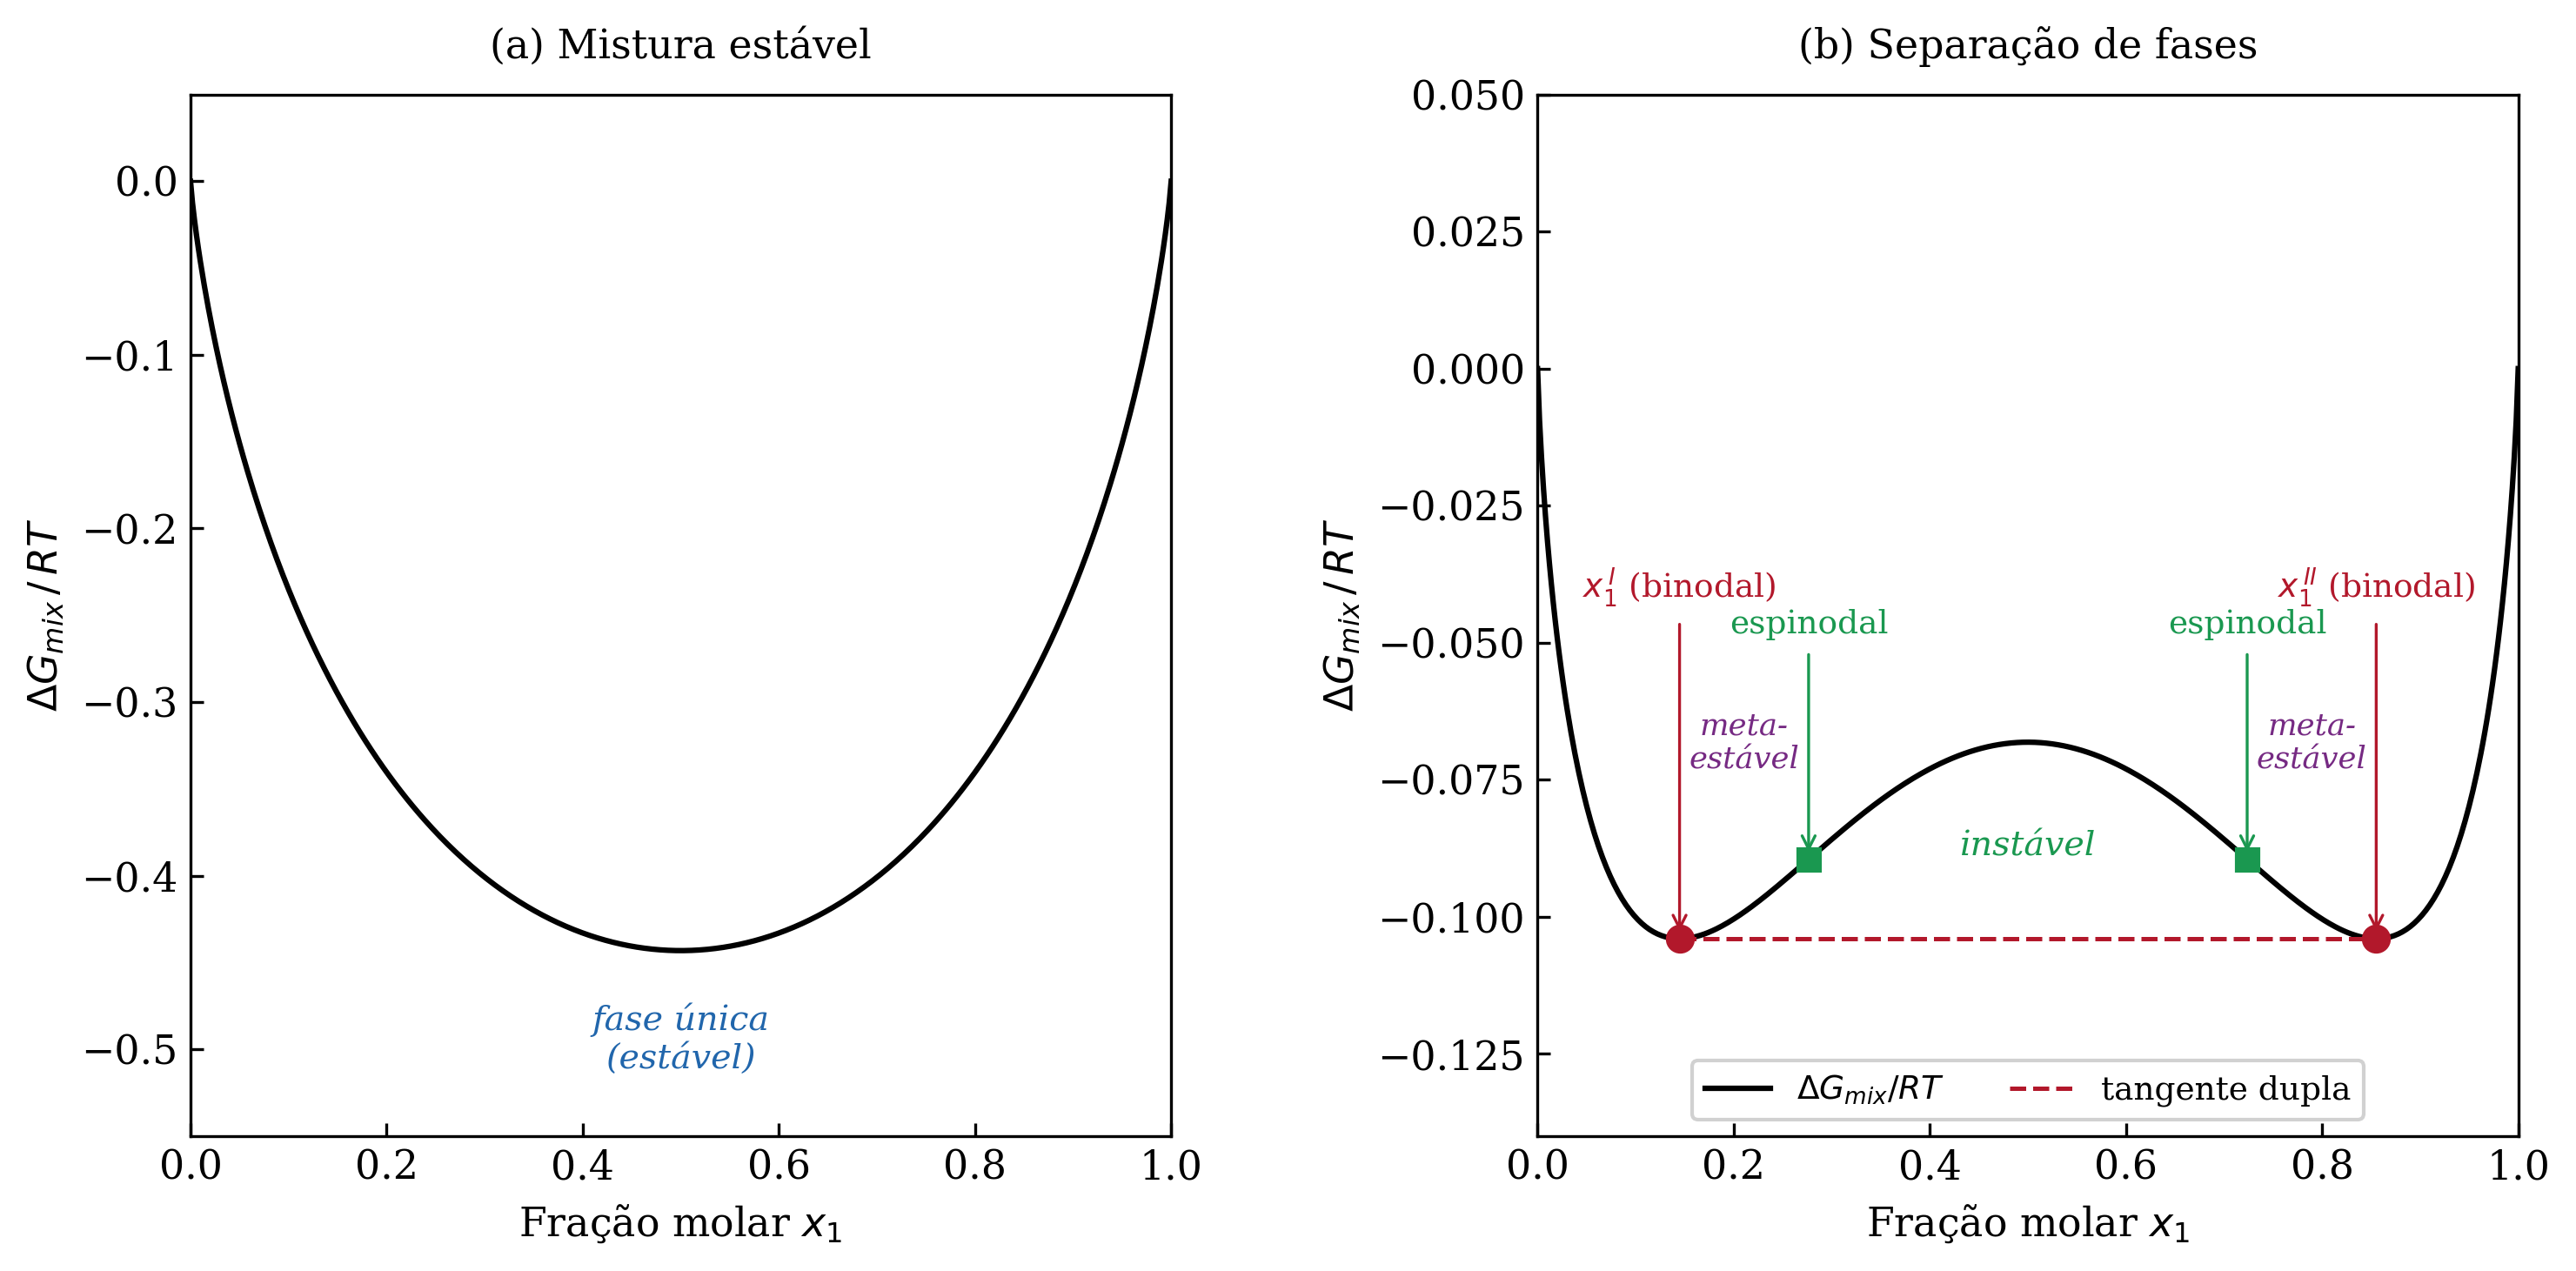
\includegraphics[width=1\linewidth]{imagens/fig1_gmix.png}
    \caption{\textit{Curva de $\Delta G_{mix}$ vs.\ composição para sistema binário, mostrando região estável, metaestável e instável, com pontos binodais e espinodais indicados.}}
    \label{fig:Curva_ΔGmix}
\end{figure}

Dessa análise decorrem duas fronteiras importantes. A curva \textit{binodal} é o lugar geométrico das composições em equilíbrio, determinadas pela tangente dupla, e delimita a região na qual o sistema se separa em duas fases. A curva \textit{espinodal}, definida pelos pontos de inflexão da curva de $\Delta G_{mix}$ (onde $\partial^2 \Delta G_{mix} / \partial x_i^2 = 0$), delimita a fronteira entre a região metaestável (entre a binodal e a espinodal, onde a mistura é localmente estável mas globalmente desfavorável) e a região instável (dentro da espinodal, onde qualquer flutuação infinitesimal de composição leva à separação espontânea). Na prática, tanto misturas metaestáveis quanto instáveis tendem a se separar, e as composições finais das fases são sempre dadas pela curva binodal\cite{smith2005}.

% -----------------------------------------------------------------
% Critério do plano tangente (TPD)
% -----------------------------------------------------------------

A construção geométrica da tangente dupla, descrita acima para o caso binário, generaliza-se para sistemas com três ou mais componentes por meio do critério do plano tangente (\textit{tangent plane distance}, TPD), formulado por \citeonline{baker1982} e sistematizado por \citeonline{michelsen1982}. Em vez de inspecionar visualmente a curvatura da superfície de energia de Gibbs, o critério TPD testa analiticamente se uma composição global $\mathbf{z}$ é estável, verificando se existe alguma composição de teste $\mathbf{x}$ capaz de reduzir a energia livre da mistura em relação ao plano tangente à superfície de $\Delta G_{mix}$ no ponto $\mathbf{z}$. A função de distância ao plano tangente é definida como\cite{michelsen1982}:

\begin{equation}
    TPD(\mathbf{x}) = \sum_{i} x_i
    \left[
        \ln(x_i \, \gamma_i(\mathbf{x})) - \ln(z_i \, \gamma_i(\mathbf{z}))
    \right]
    \label{eq:tpd}
\end{equation}

Se $TPD(\mathbf{x}) \geq 0$ para toda composição de teste $\mathbf{x}$ no espaço de composições, a mistura na composição $\mathbf{z}$ é estável como fase única. Se, ao contrário, existe algum $\mathbf{x}$ para o qual $TPD(\mathbf{x}) < 0$, a composição $\mathbf{z}$ é instável, e o sistema se separa espontaneamente em duas ou mais fases cujas composições minimizam a energia de Gibbs global\cite{michelsen1982}. Esse critério é o análogo multicomponente da condição de convexidade discutida para o caso binário (Equação~\ref{eq:gmix_total}), com a vantagem de ser diretamente aplicável a sistemas ternários como os estudados neste trabalho, nos quais a inspeção gráfica direta da superfície de $\Delta G_{mix}$ é pouco prática. A aplicação computacional do critério TPD aos sistemas ternários deste trabalho é detalhada no Capítulo~\ref{cap:metodologia}.

% -----------------------------------------------------------------
% Diagramas ternários
% -----------------------------------------------------------------

Para sistemas com três componentes, como os estudados neste trabalho, a representação do equilíbrio líquido-líquido é feita em diagramas ternários triangulares, nos quais cada vértice do triângulo equilátero corresponde a um componente puro e cada ponto no interior do triângulo representa uma composição da mistura ternária. A leitura das composições segue a convenção de que a fração molar (ou mássica) de cada componente é proporcional à distância perpendicular do ponto ao lado oposto ao vértice correspondente, de modo que a soma das três frações é sempre igual à unidade\cite{smith2005}.

\begin{figure}[H]
    \centering
    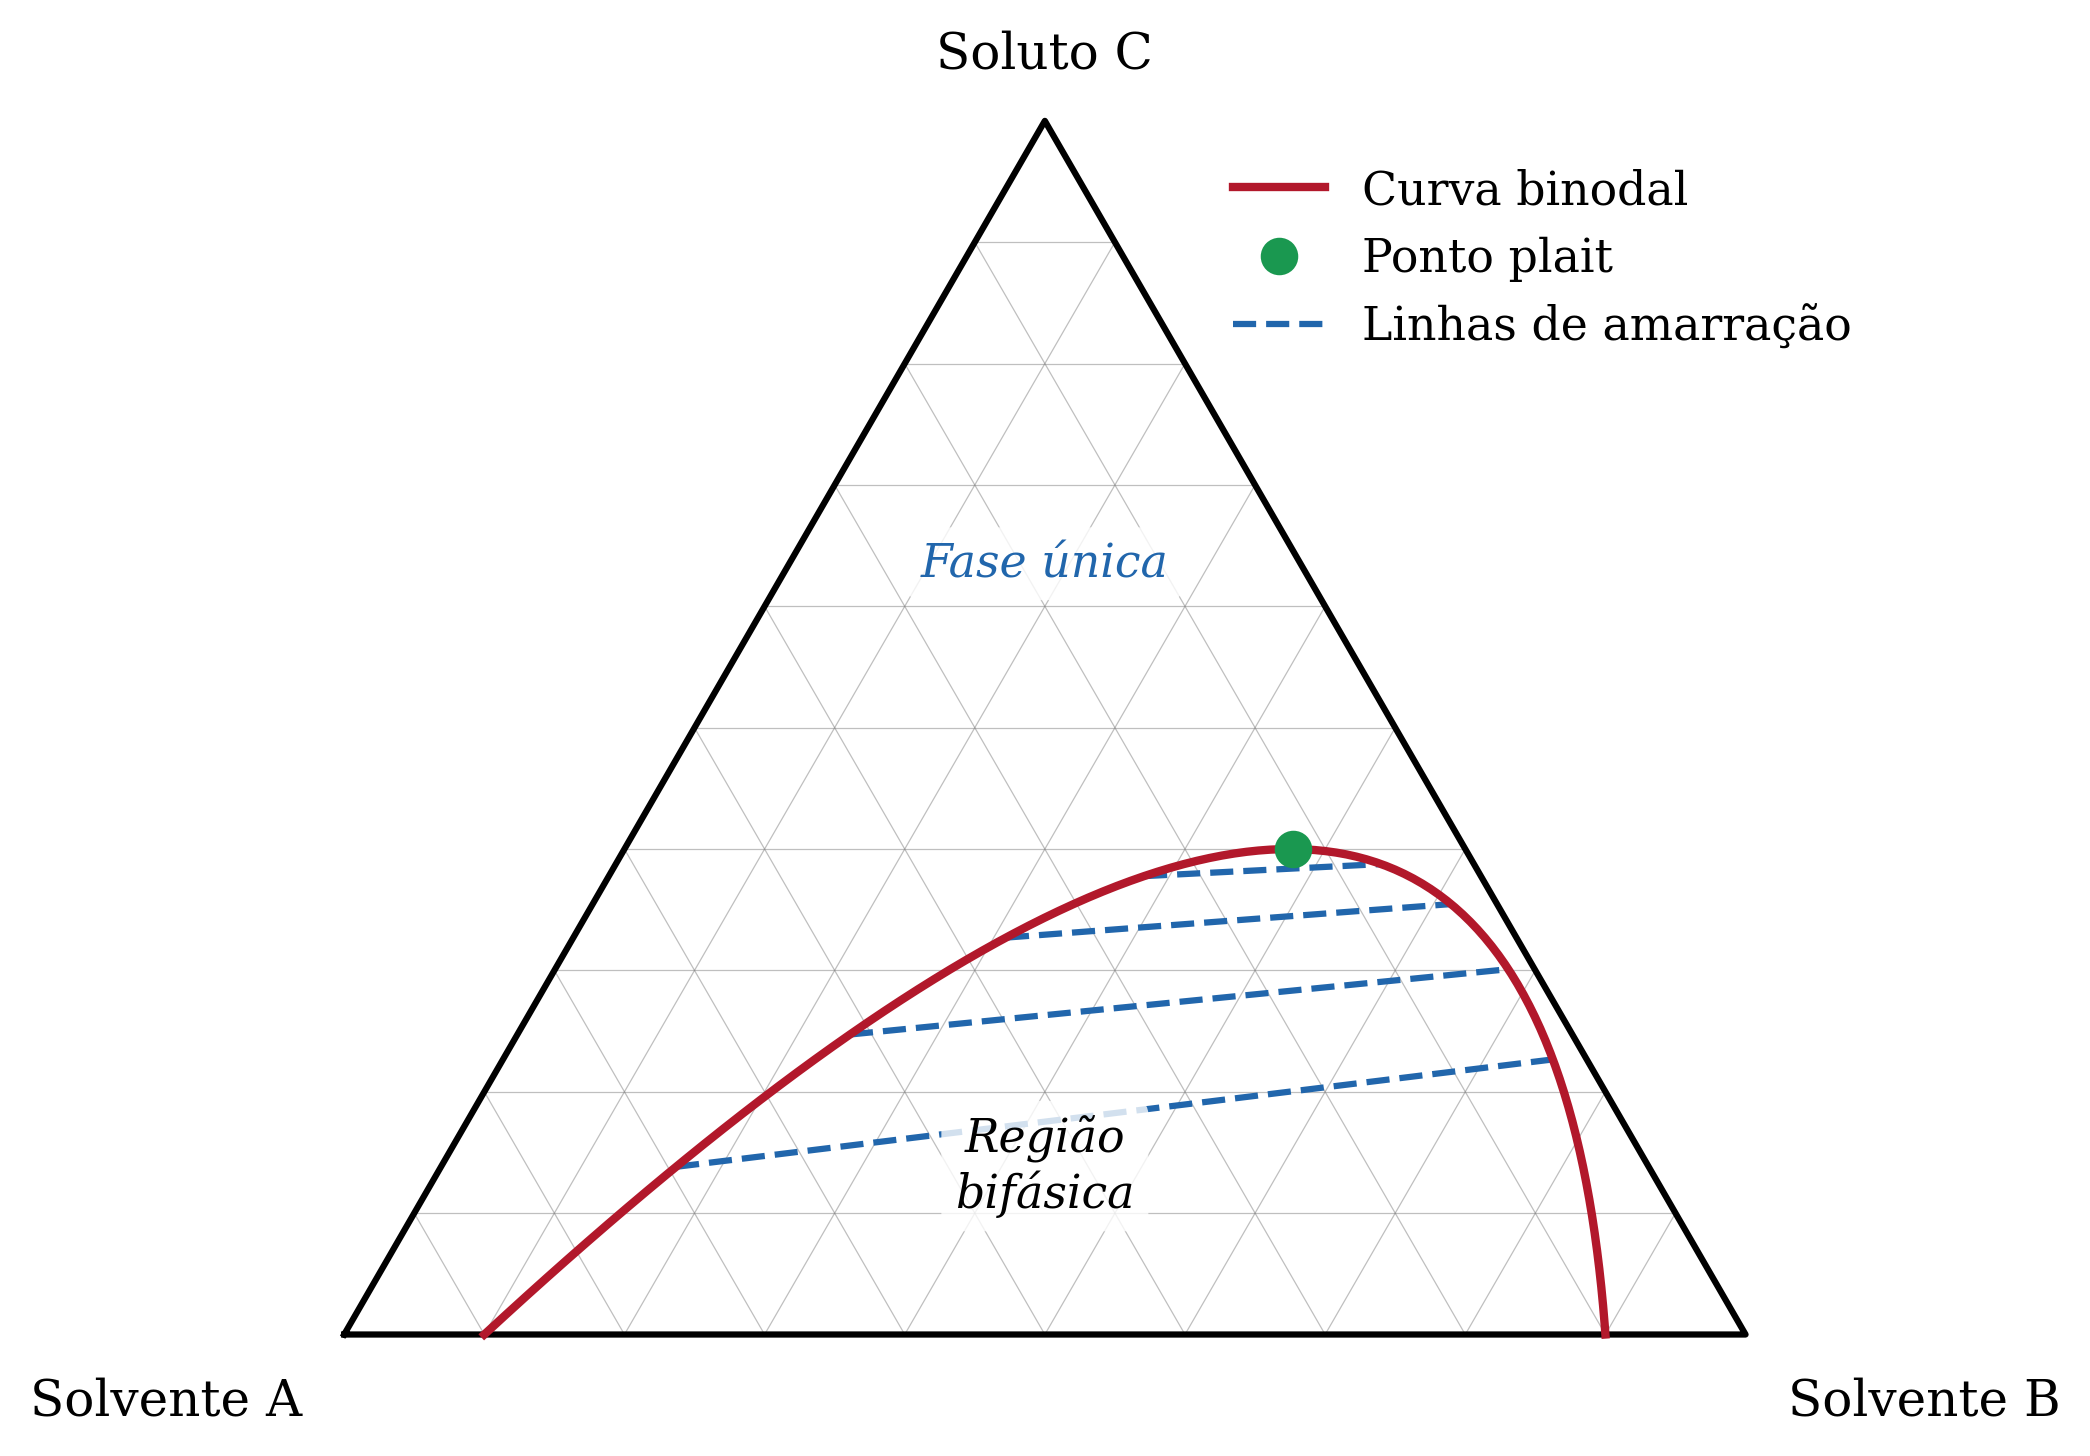
\includegraphics[width=0.8\linewidth]{imagens/fig2_diagrama_ternario.png}
    \caption{Diagrama ternário esquemático com curva binodal, linhas de amarração, ponto crítico de mistura e indicação das regiões monofásica e bifásica.}
    \label{fig:placeholder}
\end{figure}

No diagrama ternário, a região de duas fases é delimitada pela curva binodal (também denominada curva de solubilidade), que separa as composições em que o sistema existe como uma única fase líquida homogênea daquelas em que ocorre separação em duas fases. Uma composição global situada dentro da região bifásica se divide em duas fases cujas composições são dadas pelas extremidades da \textit{linha de amarração} (\textit{tie line}) que passa por aquele ponto. As linhas de amarração são segmentos de reta que conectam as composições das duas fases em equilíbrio, e sua inclinação e comprimento variam ao longo da curva binodal: à medida que se aproximam do ponto crítico de mistura (\textit{plait point}), as tie lines se tornam progressivamente mais curtas, até se reduzirem a um ponto no qual as composições e as propriedades das duas fases se tornam idênticas\cite{smith2005,treybal1980}.

Um aspecto relevante para a interpretação dos resultados deste trabalho é a relação entre a extensão da região bifásica e o efeito do cossolvente. Quando um terceiro componente (como o líquido iônico prótico) é adicionado ao sistema binário \{trioleína + etanol\}, a curva binodal se desloca, alterando a extensão da região de duas fases. Se o cossolvente aumenta a miscibilidade mútua dos reagentes, a região bifásica se contrai; se, ao contrário, o terceiro componente atua como agente de separação, a região bifásica se expande. A análise comparativa dos diagramas ternários simulados para os sistemas contendo [2-HEA][Hx] e [DETA][Hx], objetivo deste trabalho, permite avaliar quantitativamente se os LIPs são eficazes em promover a miscibilidade do sistema reacional.

As linhas de amarração fornecem ainda uma informação complementar de interesse prático: a razão de distribuição do cossolvente entre as fases. A partir das composições nas extremidades de cada tie line, pode-se calcular o coeficiente de distribuição $K_i = x_i^{II} / x_i^{I}$ de cada componente, que indica a afinidade preferencial da espécie por uma das fases\cite{treybal1980}. Para a avaliação do efeito cossolvente, a análise conjunta das tie lines e do coeficiente de distribuição do LIP permite verificar se o cossolvente se distribui entre ambas as fases ou se concentra preferencialmente em uma delas.

\section{O modelo de solvatação COSMO}
\label{sec:cosmo_solvatacao}

Os modelos da família COSMO (\textit{COnductor-like Screening MOdel}) partem de uma premissa comum: as interações intermoleculares em fase líquida podem ser descritas a partir das propriedades eletrostáticas da superfície molecular de cada espécie, calculadas individualmente por métodos de química quântica. O ponto de partida é o modelo de solvatação proposto por \citeonline{klamt1993}, posteriormente refinado por \citeonline{klamt1995}, no qual cada molécula é tratada como se estivesse imersa em um condutor perfeito. Esta seção apresenta os fundamentos desse cálculo, que constitui a etapa de entrada para o modelo COSMO-SAC discutido na Seção\ref{sec:cosmosac}.

% -----------------------------------------------------------------
% A cavidade COSMO e as cargas de blindagem
% -----------------------------------------------------------------

No modelo COSMO, a molécula de interesse é inserida em uma cavidade construída a partir dos raios de van der Waals dos átomos que a compõem. O espaço exterior à cavidade é preenchido por um condutor ideal, cuja constante dielétrica é infinita\cite{klamt1993}. Essa escolha é deliberada: em um condutor perfeito, o campo elétrico externo à cavidade é nulo, o que significa que a distribuição de cargas da molécula induz, na superfície interna da cavidade, um conjunto de cargas de blindagem (\textit{screening charges}) que cancelam exatamente o potencial eletrostático gerado pela molécula no exterior. A determinação dessas cargas de blindagem é realizada por meio de um cálculo autoconsistente de química quântica, tipicamente no formalismo da teoria do funcional da densidade (DFT), no qual a estrutura eletrônica da molécula e as cargas de blindagem na superfície são otimizadas simultaneamente até a convergência\cite{klamt1995}.

\begin{figure}[H]
    \centering
    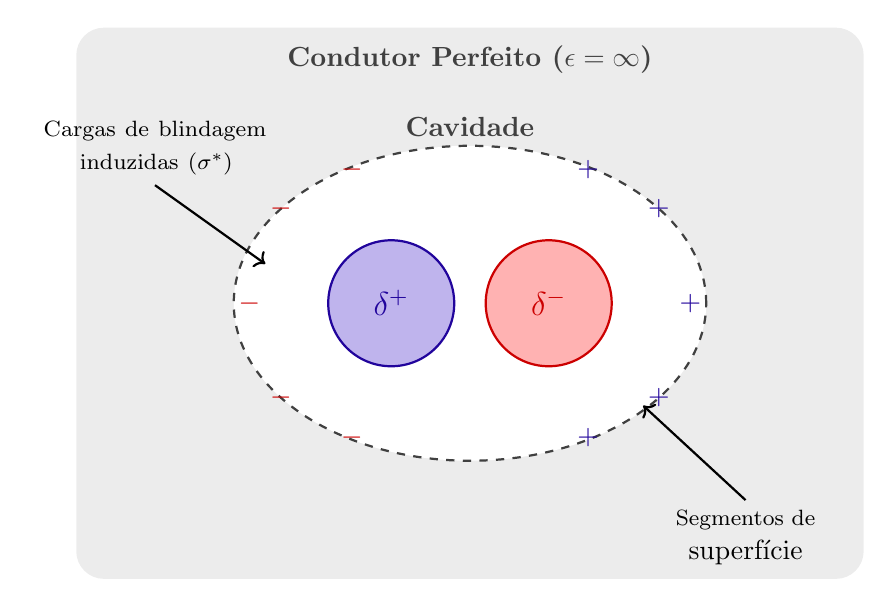
\begin{tikzpicture}
        
        % 1. Fundo representando o condutor perfeito
        % Uma caixa cinza com bordas arredondadas
        \fill[gray!15, rounded corners=10pt] (-5,-3.5) rectangle (5,3.5);
        \node[above, darkgray] at (0, 2.8) {\textbf{Condutor Perfeito ($\epsilon = \infty$)}};

        % 2. A Cavidade COSMO
        % Desenhada como uma elipse branca com borda tracejada
        \fill[white] (0,0) ellipse (3cm and 2cm);
        \draw[thick, dashed, darkgray] (0,0) ellipse (3cm and 2cm);
        
        % Label da cavidade
        \node[above, darkgray] at (0, 2) {\textbf{Cavidade}};

        % 3. Molécula Genérica (Dipolo)
        % Átomo com carga parcial positiva (Azul)
        \fill[blue!30] (-1,0) circle (0.8cm);
        \draw[thick, blue!80!black] (-1,0) circle (0.8cm);
        \node[blue!80!black] at (-1, 0) {\large $\delta^+$};
        
        % Átomo com carga parcial negativa (Vermelho)
        \fill[red!30] (1,0) circle (0.8cm);
        \draw[thick, red!80!black] (1,0) circle (0.8cm);
        \node[red!80!black] at (1, 0) {\large $\delta^-$};

        % 4. Segmentos de Superfície e Cargas de Triagem (\sigma)
        % Cargas negativas induzidas próximas ao polo positivo da molécula
        \node[red!80!black, font=\bfseries] at (-2.8, 0) {$-$};
        \node[red!80!black, font=\bfseries] at (-2.4, 1.2) {$-$};
        \node[red!80!black, font=\bfseries] at (-2.4, -1.2) {$-$};
        \node[red!80!black, font=\bfseries] at (-1.5, 1.7) {$-$};
        \node[red!80!black, font=\bfseries] at (-1.5, -1.7) {$-$};

        % Cargas positivas induzidas próximas ao polo negativo da molécula
        \node[blue!80!black, font=\bfseries] at (2.8, 0) {$+$};
        \node[blue!80!black, font=\bfseries] at (2.4, 1.2) {$+$};
        \node[blue!80!black, font=\bfseries] at (2.4, -1.2) {$+$};
        \node[blue!80!black, font=\bfseries] at (1.5, 1.7) {$+$};
        \node[blue!80!black, font=\bfseries] at (1.5, -1.7) {$+$};

        % 5. Setas e Rótulos Explicativos
        % Seta apontando para as cargas de triagem
        \draw[<-, thick] (-2.6, 0.5) -- (-4, 1.5) 
            node[above, align=center, text width=3cm] {\footnotesize Cargas de blindagem induzidas ($\sigma^*$)};
            
        % Seta apontando para a fronteira (segmentos)
        \draw[<-, thick] (2.2, -1.3) -- (3.5, -2.5) 
            node[below, align=center] {\footnotesize Segmentos de\\superfície};

    \end{tikzpicture}
    \vspace{0.5cm}
    \caption{Representação esquemática do modelo COSMO mostrando
    a molécula na cavidade, o condutor perfeito e os segmentos de
    superfície com suas cargas de blindagem. Adaptado de Lin e Sandler (2002).}
    \label{fig:cosmo_cavity}
\end{figure}

O resultado do cálculo COSMO é uma superfície molecular discretizada em $n$ segmentos, cada um caracterizado por uma área $a_n$ e uma densidade de carga de blindagem $\sigma_n^{*}$ (em unidades de carga por unidade de área, tipicamente e/\AA$^2$). Essa distribuição de cargas na superfície reflete, de forma compacta, toda a informação relevante sobre a capacidade da molécula de interagir eletrostaticamente com o meio ao seu redor: regiões da superfície com $\sigma > 0$ correspondem a segmentos onde a molécula apresenta carga negativa exposta (e o condutor responde com carga positiva de blindagem), enquanto regiões com $\sigma < 0$ indicam carga positiva na superfície molecular. Segmentos com $\sigma \approx 0$ correspondem a regiões apolares da molécula\cite{lin2002}. 
% -----------------------------------------------------------------
% Do condutor perfeito ao solvente real
% -----------------------------------------------------------------

Uma observação importante é que o cálculo COSMO descreve a molécula em um condutor perfeito, e não em um solvente real. A transição do condutor ideal para um meio dielétrico finito (como um líquido) requer uma correção, que nos modelos da família COSMO é feita por meio de um fator de escala aplicado às cargas de blindagem\cite{klamt1995}. Essa correção, embora conceitualmente relevante, não altera a estrutura do cálculo: o procedimento continua sendo resolver a equação de Schrödinger-Kohn-Sham na presença do contínuo dielétrico e extrair as cargas de superfície. Os detalhes do nível de teoria empregado (funcional DFT e conjunto de funções de base), que influenciam a qualidade das cargas obtidas, são discutidos no Capítulo\ref{cap:metodologia} no contexto específico dos compostos estudados neste trabalho.

% -----------------------------------------------------------------
% Perfis de densidade de carga superficial (σ-profiles)
% -----------------------------------------------------------------

A representação tridimensional das cargas de blindagem sobre a superfície molecular (denominada $\sigma$-\textit{surface}) contém toda a informação necessária, porém não é diretamente utilizável nos cálculos de equilíbrio de fases, que requerem uma descrição estatística das interações entre segmentos. Para viabilizar essa descrição, a distribuição de cargas é projetada em um histograma unidimensional denominado \textit{perfil de densidade de carga superficial}, ou $\sigma$-\textit{profile}, designado por $p_i(\sigma)$\cite{lin2002}. O $\sigma$-profile de uma substância $i$ representa a distribuição de área superficial da molécula em função da densidade de carga $\sigma$:

\begin{equation}
    p_i(\sigma) = \frac{A_i(\sigma)}{A_i}
    \label{eq:sigma_profile}
\end{equation}

\noindent em que $A_i(\sigma)$ é a área total dos segmentos que possuem densidade de carga $\sigma$ e $A_i$ é a área total da cavidade da molécula $i$.

Antes de construir o histograma, contudo, as cargas brutas provenientes do cálculo COSMO ($\sigma_n^{*}$) passam por um procedimento de suavização (\textit{averaging}), no qual a carga de cada segmento é recalculada como uma média ponderada das cargas dos segmentos vizinhos. Essa etapa é necessária porque o modelo COSMO-SAC assume que todos os segmentos possuem a mesma área efetiva $a_{eff}$, e a suavização garante que a distribuição de cargas seja consistente com essa premissa\cite{lin2002}. O raio de suavização $r_{eff}$ é um dos parâmetros universais do modelo.

\begin{figure}[H]
    \centering
    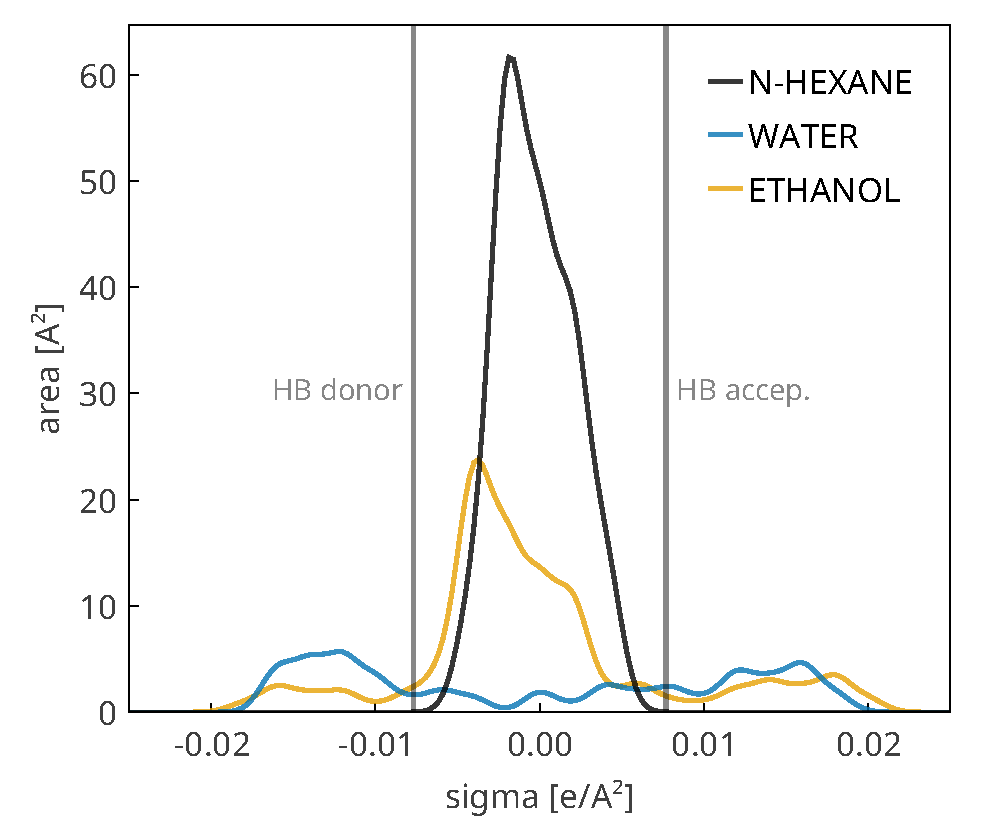
\includegraphics[width=0.5\textwidth]{imagens/N-HEXANE-WATER-ETHANOL.pdf}
    \caption{$\sigma$-\textit{profiles} de n-hexano, água e etanol, gerados no JCOSMO com a base GAMESS. As linhas verticais delimitam as regiões de doação (HB \textit{donor},  $\sigma < -0{,}0082$ e/\AA$^2$) e aceitação (HB \textit{accep.}, $\sigma > +0{,}0082$ e/\AA$^2$) de ligações de hidrogênio. A região central ($|\sigma| < 0{,}0082$ e/\AA$^2$) corresponde a segmentos apolares.
    Fonte: gerado no \textit{software} JCOSMO.}
    \label{fig:sigma_profiles}
\end{figure}
A interpretação física do $\sigma$-profile é direta e constitui uma das vantagens conceituais dos modelos baseados em COSMO. A região central do perfil ($\sigma \approx 0$) corresponde à área apolar da molécula, que interage com o meio apenas por forças de dispersão fracas. As regiões com $\sigma$ fortemente positivo (tipicamente $\sigma > +0{,}01$ e/\AA$^2$) correspondem a segmentos com carga negativa exposta na superfície molecular, como os pares de elétrons não ligantes de átomos de oxigênio ou nitrogênio, que são aceptores de ligações de hidrogênio. Simetricamente, as regiões com $\sigma$ fortemente negativo ($\sigma < -0{,}01$ e/\AA$^2$) correspondem a segmentos com carga positiva exposta, como os hidrogênios ligados a átomos eletronegativos, que são doadores de ligações de hidrogênio\cite{lin2002}. Dessa forma, uma molécula apolar como o hexano apresenta um $\sigma$-profile concentrado em torno de $\sigma = 0$, enquanto uma molécula como a água apresenta dois picos pronunciados nas regiões de doação e aceitação de hidrogênio. O etanol, por possuir tanto uma cadeia alquílica apolar quanto um grupo hidroxila, exibe um perfil intermediário com contribuições nas três regiões\cite{lin2002}.

Essa representação será particularmente útil na discussão dos resultados (Capítulo\ref{cap:resultados}), pois a comparação dos $\sigma$-profiles dos cátions [2-HEA]$^+$ e [DETA]$^+$ e do ânion [Hx]$^-$ permite identificar, em termos moleculares, as diferenças de interação que explicam o comportamento distinto dos dois LIPs como cossolventes no sistema \{trioleína + etanol\}.

\section{O modelo COSMO-SAC}
\label{sec:cosmosac}

O modelo COSMO-SAC (\textit{COnductor-like Screening MOdel -- Segment Activity Coefficient}) foi proposto por \citeonline{lin2002} como uma variação do modelo COSMO-RS (\textit{COSMO for Real Solvents}),  introduzido por \citeonline{klamt1995}. Ambos os modelos compartilham a premissa de que as interações intermoleculares em fase líquida podem ser calculadas a partir dos $\sigma$-profiles das espécies puras, sem necessidade de parâmetros ajustados a dados experimentais de misturas. A diferença reside na formulação termodinâmica empregada: enquanto o COSMO-RS utiliza uma expressão analítica direta para o potencial químico dos segmentos, o COSMO-SAC reformula o problema em termos de coeficientes de atividade de segmento, dentro de um arcabouço compatível com os modelos clássicos de $G^E$ utilizados em engenharia química\cite{lin2002,gerber2010}.

% -----------------------------------------------------------------
% Estrutura geral do coeficiente de atividade
% -----------------------------------------------------------------

No COSMO-SAC, o coeficiente de atividade do componente $i$ em uma solução $S$ é expresso como a soma de duas contribuições\cite{lin2002}:

\begin{equation}
    \ln \gamma_i = \ln \gamma_i^{comb} + \ln \gamma_i^{res}
    \label{eq:gamma_cosmo}
\end{equation}

A contribuição residual ($\ln \gamma_i^{res}$) captura os efeitos das interações eletrostáticas e de ligações de hidrogênio entre os segmentos de superfície, e é calculada a partir dos $\sigma$-profiles. A contribuição combinatorial ($\ln \gamma_i^{comb}$) descreve os efeitos entrópicos associados às diferenças de tamanho e forma entre as moléculas da mistura, e é calculada a partir do volume e da área da cavidade COSMO de cada espécie. As duas contribuições são apresentadas a seguir.

% -----------------------------------------------------------------
% Contribuição residual
% -----------------------------------------------------------------

\subsection{Contribuição residual: interações entre segmentos de
superfície}
\label{subsec:cosmo_residual}

A contribuição residual ao coeficiente de atividade é obtida a partir da diferença entre a energia livre de restauração (\textit{restoring free energy}) do soluto $i$ na mistura $S$ e no líquido puro\cite{lin2002}:

\begin{equation}
    \ln \gamma_i^{res} =
    \frac{\Delta G_i^{*res/S} - \Delta G_i^{*res/i}}{RT}
    \label{eq:gamma_residual}
\end{equation}

A energia livre de restauração representa o custo energético de ``religar'' as interações eletrostáticas da molécula quando ela é transferida do condutor perfeito (onde as cargas estão perfeitamente blindadas) para o meio líquido real (onde a blindagem é imperfeita)\cite{lin2002}. A diferença entre os dois termos na Equação\ref{eq:gamma_residual} garante que, quando o soluto se encontra em seu próprio líquido puro, $\ln \gamma_i^{res} = 0$, como esperado. A energia livre de restauração é calculada como uma soma sobre todos os segmentos da molécula $i$, ponderada pelo $\sigma$-profile da espécie e pelo coeficiente de atividade de cada tipo de segmento\cite{lin2002}:

\begin{equation}
    \frac{\Delta G_i^{*res/S}}{RT} =
    n_i \sum_{\sigma_m} p_i(\sigma_m) \, \ln \Gamma_S(\sigma_m)
    \label{eq:energia_restauracao}
\end{equation}

\noindent em que $n_i = A_i / a_{eff}$ é o número total de segmentos na superfície da molécula $i$, $p_i(\sigma_m)$ é o $\sigma$-profile da espécie pura $i$ e $\Gamma_S(\sigma_m)$ é o coeficiente de atividade do segmento com carga $\sigma_m$ na mistura $S$.

O coeficiente de atividade de segmento $\Gamma_S(\sigma_m)$ é o elemento central do modelo. Ele mede o quanto um segmento de carga $\sigma_m$ se desvia do comportamento ideal na mistura, e é obtido pela solução da seguinte equação implícita\cite{lin2002}:

\begin{equation}
    \ln \Gamma_S(\sigma_m) =
    -\ln \left\{
        \sum_{\sigma_n} p_S(\sigma_n) \, \Gamma_S(\sigma_n)
        \exp \left[
            -\frac{\Delta W(\sigma_m, \sigma_n)}{RT}
        \right]
    \right\}
    \label{eq:gamma_segmento}
\end{equation}

\noindent em que $p_S(\sigma_n)$ é o $\sigma$-profile da mistura $S$ e $\Delta W(\sigma_m, \sigma_n)$ é a energia de interação entre um par de segmentos com cargas $\sigma_m$ e $\sigma_n$. A Equação\ref{eq:gamma_segmento} é implícita porque $\Gamma_S(\sigma_m)$
aparece em ambos os lados, e deve ser resolvida iterativamente até a convergência\cite{lin2002}.

O $\sigma$-profile da mistura é construído como a média ponderada dos $\sigma$-profiles dos componentes puros, utilizando as frações molares como pesos\cite{lin2002}:

\begin{equation}
    p_S(\sigma) = \sum_{i=1}^{c} x_i \, p_i(\sigma)
    \label{eq:sigma_profile_mistura}
\end{equation}

Essa expressão reflete uma das hipóteses centrais do modelo: os segmentos de superfície são tratados como independentes e a composição da ``superfície da mistura'' é simplesmente a soma das superfícies de cada componente, ponderada pela composição\cite{lin2002}.

% -----------------------------------------------------------------
% Energia de interação entre segmentos
% -----------------------------------------------------------------

\subsection{Energia de interação entre segmentos}
\label{subsec:cosmo_interacao}

A energia de interação entre dois segmentos de superfície com densidades de carga $\sigma_m$ e $\sigma_n$ é composta por duas contribuições\cite{lin2002}:

\begin{equation}
    \Delta W(\sigma_m, \sigma_n) =
    \Delta W_{mf}(\sigma_m, \sigma_n)
    + \Delta W_{hb}(\sigma_m, \sigma_n)
    \label{eq:energia_interacao}
\end{equation}

A primeira contribuição é a energia de \textit{misfit} (desajuste eletrostático), que penaliza o contato entre segmentos cujas cargas de blindagem não se cancelam mutuamente:

\begin{equation}
    \Delta W_{mf}(\sigma_m, \sigma_n) =
    \frac{R'}{2} (\sigma_m + \sigma_n)^2
    \label{eq:energia_misfit}
\end{equation}

\noindent em que $R'$ é uma constante que depende do fator de polarização $f_{pol}$ e da área efetiva de segmento $a_{eff}$. O termo $(\sigma_m + \sigma_n)^2$ tem um significado físico intuitivo: quando dois segmentos com cargas opostas entram em contato ($\sigma_m + \sigma_n \approx 0$), a energia de misfit é mínima, pois as cargas se cancelam mutuamente, assim como ocorreria no condutor perfeito. Quando dois segmentos de mesma carga se encontram, a soma é grande e a penalidade energética é máxima, refletindo a situação desfavorável em que a blindagem é deficiente\cite{lin2002}.

A segunda contribuição é a energia de ligação de hidrogênio, que estabiliza o contato entre segmentos doadores e aceptores de ligações de hidrogênio\cite{lin2002}:

\begin{equation}
    \Delta W_{hb}(\sigma_m, \sigma_n) =
    c_{hb} \,
    \max\!\left[0, \;\sigma_{acc} - \sigma_{hb}\right]
    \cdot
    \min\!\left[0, \;\sigma_{don} + \sigma_{hb}\right]
    \label{eq:energia_hbond}
\end{equation}

\noindent em que $c_{hb}$ é a constante de ligação de hidrogênio, $\sigma_{hb}$ é o valor de corte que define quais segmentos são capazes de participar de ligações de hidrogênio, e $\sigma_{acc}$ e $\sigma_{don}$ são, respectivamente, o maior e o menor valor entre $\sigma_m$ e $\sigma_n$. A Equação\ref{eq:energia_hbond} é construída de modo que a contribuição de ligação de hidrogênio seja não nula apenas quando um segmento fortemente positivo ($\sigma_{acc} > \sigma_{hb}$, aceptor) interage com um segmento fortemente negativo ($\sigma_{don} < -\sigma_{hb}$, doador). Nesse caso, o produto é negativo, reduzindo a energia total de interação e estabilizando o contato\cite{lin2002}. Para pares de segmentos que não satisfazem o critério de corte, a contribuição de ligação de hidrogênio é nula.

% -----------------------------------------------------------------
% Extensão HB2: subdivisão da superfície de ligação de hidrogênio
% -----------------------------------------------------------------

A formulação original de \citeonline{lin2002}, apresentada na Equação~\ref{eq:energia_hbond}, trata toda a superfície capaz de participar de ligações de hidrogênio de forma homogênea, com uma única constante $c_{hb}$ e um único valor de corte $\sigma_{hb}$. \citeonline{hsieh2010} propuseram um refinamento desse tratamento, denominado COSMO-SAC-HB2 (ou COSMO-SAC-2010), no qual os segmentos de superfície capazes de participar de ligações de hidrogênio são subdivididos em dois tipos: segmentos associados a grupos hidroxila (tipo OH) e segmentos associados a outros grupos doadores ou aceptores de hidrogênio, como nitrogênio, oxigênio não hidroxílico e flúor (tipo OT). Essa subdivisão reflete a observação empírica de que a intensidade da ligação de hidrogênio varia conforme o tipo químico do grupo envolvido, e não apenas conforme a magnitude da densidade de carga do segmento.

Na prática, essa subdivisão se propaga por todo o formalismo do COSMO-SAC: o $\sigma$-profile de cada espécie pura, antes descrito por uma única distribuição $p_i(\sigma)$ (Equação~\ref{eq:sigma_profile}), passa a ser decomposto em três distribuições parciais,
\begin{equation}
    p_i(\sigma) = p_i^{nhb}(\sigma) + p_i^{OH}(\sigma) + p_i^{OT}(\sigma),
    \label{eq:sigma_profile_hb2}
\end{equation}
correspondentes, respectivamente, aos segmentos sem capacidade de ligação de hidrogênio, aos segmentos do tipo OH e aos segmentos do tipo OT. A energia de interação entre dois segmentos (Equação~\ref{eq:energia_hbond}) passa a depender não apenas das densidades de carga $\sigma_m$ e $\sigma_n$, mas também dos tipos $t_m, t_n \in \{OH, OT\}$ de cada segmento, por meio de uma constante de ligação de hidrogênio específica para cada combinação de tipos:
\begin{equation}
    \Delta W_{hb}(\sigma_m, \sigma_n) =
    c_{hb}^{(t_m, t_n)} \,
    \max\!\left[0, \;\sigma_{acc} - \sigma_{hb}\right]
    \cdot
    \min\!\left[0, \;\sigma_{don} + \sigma_{hb}\right],
    \label{eq:energia_hbond_hb2}
\end{equation}
em que $c_{hb}^{(OH,OH)}$, $c_{hb}^{(OT,OT)}$ e $c_{hb}^{(OH,OT)}$ são três constantes distintas, ajustadas por \citeonline{hsieh2010} a um banco de dados experimental de equilíbrio de fases mais amplo do que o utilizado na parametrização original de \citeonline{lin2002}. O valor de corte $\sigma_{hb}$ permanece único, comum aos dois tipos de segmento. Essa subdivisão permite, por exemplo, que a interação entre dois segmentos hidroxila (como em uma ligação O–H\textperiodcentered\textperiodcentered\textperiodcentered O entre duas moléculas de álcool) seja tratada com uma intensidade diferente da interação entre um segmento hidroxila e um segmento amino (como ocorre entre o álcool e o líquido iônico prótico nos sistemas estudados neste trabalho, Seção~\ref{subsec:ligacao_hidrogenio}), refinamento particularmente relevante para a diversidade de grupos doadores e aceptores de hidrogênio presentes nos sistemas \{triglicerídeo + álcool + líquido iônico prótico\} deste trabalho. A parametrização COSMO-SAC-HB2 é a efetivamente empregada nos cálculos deste trabalho (Capítulo~\ref{cap:metodologia}), e as demais equações do modelo (contribuição combinatorial, energia de misfit) permanecem inalteradas em relação à formulação original.

% -----------------------------------------------------------------
% Contribuição combinatorial
% -----------------------------------------------------------------

\subsection{Contribuição combinatorial: efeitos de tamanho e forma}
\label{subsec:cosmo_combinatorial}

A contribuição combinatorial ao coeficiente de atividade é calculada pelo modelo de Staverman-Guggenheim, que descreve os efeitos entrópicos decorrentes das diferenças de tamanho e forma entre as moléculas da mistura\cite{lin2002}:

\begin{equation}
    \ln \gamma_i^{comb} =
    \ln \frac{\phi_i}{x_i}
    + \frac{z}{2} \, q_i \, \ln \frac{\theta_i}{\phi_i}
    + l_i
    - \frac{\phi_i}{x_i} \sum_{j} x_j \, l_j
    \label{eq:gamma_combinatorial}
\end{equation}

\noindent em que $z = 10$ é o número de coordenação da rede, $\phi_i = r_i x_i / \sum_j r_j x_j$ é a fração volumétrica normalizada, $\theta_i = q_i x_i / \sum_j q_j x_j$ é a fração de área superficial normalizada, e $l_i = (z/2)(r_i - q_i) - (r_i - 1)$. Os parâmetros $r_i$ e $q_i$ são, respectivamente, o volume e a área superficial normalizados da molécula $i$, obtidos diretamente da cavidade COSMO\cite{lin2002}:

\begin{equation}
    r_i = \frac{V_i}{r_{std}} \qquad \text{e} \qquad
    q_i = \frac{A_i}{q_{std}}
    \label{eq:ri_qi}
\end{equation}

\noindent em que $V_i$ e $A_i$ são o volume e a área total da cavidade COSMO da molécula $i$, e $r_{std}$ e $q_{std}$ são parâmetros universais de normalização. A contribuição combinatorial tende a ser mais significativa em misturas de moléculas com tamanhos muito diferentes, como é o caso do sistema \{trioleína + etanol\}, em que a trioleína (\ce{C57H104O6}, massa molar 885,4g/mol) é consideravelmente maior que o etanol (\ce{C2H6O}, massa molar 46,1g/mol).

% -----------------------------------------------------------------
% Parâmetros universais
% -----------------------------------------------------------------

\subsection{Parâmetros universais do modelo}
\label{subsec:cosmo_parametros}

Um aspecto importante do COSMO-SAC é que o modelo depende de um conjunto reduzido de parâmetros universais, que são ajustados uma única vez a partir de um banco de dados de propriedades termodinâmicas e permanecem fixos para qualquer sistema subsequente. Os principais parâmetros são a área efetiva de segmento $a_{eff}$ (que define o tamanho dos segmentos no procedimento de suavização), o raio de suavização $r_{eff}$, o fator de polarização $f_{pol}$, a constante de ligação de hidrogênio $c_{hb}$, o valor de corte $\sigma_{hb}$ e os parâmetros de normalização $r_{std}$ e $q_{std}$\cite{lin2002,gerber2010}. Os valores numéricos desses parâmetros dependem do nível de teoria utilizado na geração dos $\sigma$-profiles (isto é, do pacote de química quântica empregado), e diferentes parametrizações foram propostas na literatura para $\sigma$-profiles gerados com DMol3, GAMESS, MOPAC e TURBOMOLE\cite{gerber2010}. A consistência entre o nível de teoria dos cálculos COSMO e a parametrização do modelo é essencial para a qualidade das predições, como discutido por
\citeonline{gerber2010}, e constitui um aspecto central da metodologia adotada neste trabalho (Capítulo\ref{cap:metodologia}).

O fato de esses parâmetros serem universais (isto é, não específicos para cada sistema ou mistura) é o que confere ao COSMO-SAC sua natureza preditiva \textit{a priori}: uma vez calibrado o modelo com uma base de dados de referência, qualquer sistema pode ser tratado desde que os $\sigma$-profiles dos componentes estejam disponíveis. Não há necessidade de parâmetros binários de interação ajustados a dados experimentais da mistura de interesse, ao contrário do que ocorre nos modelos de contribuição por grupos como o UNIFAC-LL, discutido na Seção\ref{sec:unifacll}.

\section{Tratamento de líquidos iônicos no formalismo COSMO}
\label{sec:cosmo_li}

O modelo COSMO-SAC, tal como formulado por \citeonline{lin2002}, foi desenvolvido e parametrizado para misturas de moléculas neutras. A aplicação do modelo a sistemas contendo líquidos iônicos introduz uma dificuldade conceitual que não se apresenta para compostos moleculares convencionais: o LI é composto por dois íons (cátion e ânion), e a forma como essas espécies são representadas no cálculo COSMO afeta diretamente os $\sigma$-profiles gerados e, consequentemente, a qualidade das predições de equilíbrio de fases. Duas estratégias principais foram propostas na literatura para lidar com essa questão, denominadas abordagem CA (par iônico) e abordagem C+A (íons separados)\cite{dominguez2014}.

% -----------------------------------------------------------------
% Abordagem CA: par iônico neutro
% -----------------------------------------------------------------

Na abordagem CA, o cátion e o ânion são tratados como uma única entidade neutra. O cálculo COSMO é realizado sobre o par iônico, gerando um único $\sigma$-profile que representa o LI como se fosse uma molécula convencional\cite{dominguez2014}. Essa estratégia tem a vantagem da simplicidade, pois permite utilizar o formalismo COSMO-SAC sem qualquer modificação. Apresenta, contudo, duas limitações relevantes. A primeira é a arbitrariedade da geometria: o par iônico pode adotar diversas orientações relativas entre cátion e ânion, e a geometria escolhida para o cálculo influencia a distribuição de cargas na superfície e, portanto, o $\sigma$-profile resultante. A segunda limitação é de natureza física: em fase líquida, os íons de um LI não permanecem necessariamente associados como pares fixos, de modo que a representação como par iônico é uma simplificação que pode não capturar adequadamente as interações individuais de cada íon com as demais espécies da mistura\cite{dominguez2014}.

% -----------------------------------------------------------------
% Abordagem C+A: íons separados
% -----------------------------------------------------------------

Na abordagem C+A, o cátion e o ânion são tratados como espécies independentes. Os cálculos COSMO são realizados separadamente para cada íon, gerando $\sigma$-profiles individuais ($p_C(\sigma)$ para o cátion e $p_A(\sigma)$ para o ânion). O $\sigma$-profile do LI é então construído como uma média ponderada dos perfis das duas espécies iônicas, utilizando
as respectivas áreas superficiais como pesos\cite{dominguez2014}:

\begin{equation}
    p_{LI}(\sigma) =
    \frac{x_C \, A_C \, p_C(\sigma) \;+\; x_A \, A_A \, p_A(\sigma)}
         {x_C \, A_C \;+\; x_A \, A_A}
    \label{eq:sigma_profile_ca}
\end{equation}

\noindent em que $x_C$ e $x_A$ são as frações molares do cátion e do ânion (ambas iguais a 0,5 para um LI monovalente do tipo 1:1), e $A_C$ e $A_A$ são as áreas superficiais totais das respectivas cavidades COSMO. De forma análoga, o volume e a área normalizados do LI ($r_{LI}$ e $q_{LI}$), necessários para a contribuição combinatorial (Equação\ref{eq:gamma_combinatorial}), são obtidos pela soma das contribuições individuais de cada íon\cite{dominguez2014}:

\begin{equation}
    r_{LI} = r_C + r_A \qquad \text{e} \qquad q_{LI} = q_C + q_A
    \label{eq:rq_li}
\end{equation}

Essa abordagem elimina a arbitrariedade geométrica do par iônico, uma vez que cada íon é calculado individualmente em sua própria cavidade COSMO. Além disso, a representação como íons separados é mais consistente com a natureza dissociada do LI em fase líquida, na qual os íons interagem de forma relativamente independente com as moléculas do solvente\cite{dominguez2014}.

% -----------------------------------------------------------------
% Evidência da literatura e escolha da abordagem
% -----------------------------------------------------------------

% -----------------------------------------------------------------
% Evidência da literatura e escolha da abordagem
% -----------------------------------------------------------------

A comparação entre as duas abordagens foi realizada por \citeonline{dominguez2014}, que aplicaram o modelo COSMO-RS à predição do ELL de sistemas ternários \{hidrocarboneto alifático + hidrocarboneto aromático + LI de imidazólio\} a 298,15~K. Os autores verificaram que a abordagem C+A fornece predições quantitativamente superiores às da abordagem CA para a maioria dos sistemas estudados, com melhor descrição tanto da inclinação das linhas de amarração quanto da extensão da região bifásica\cite{dominguez2014}. Resultados consistentes com essa conclusão foram obtidos por \citeonline{xu2022}, que empregaram o COSMO-SAC na predição de ELL de sistemas \{éster + álcool + LI de imidazólio\} e adotaram a abordagem C+A como padrão.

\begin{figure}[H]
    \centering
    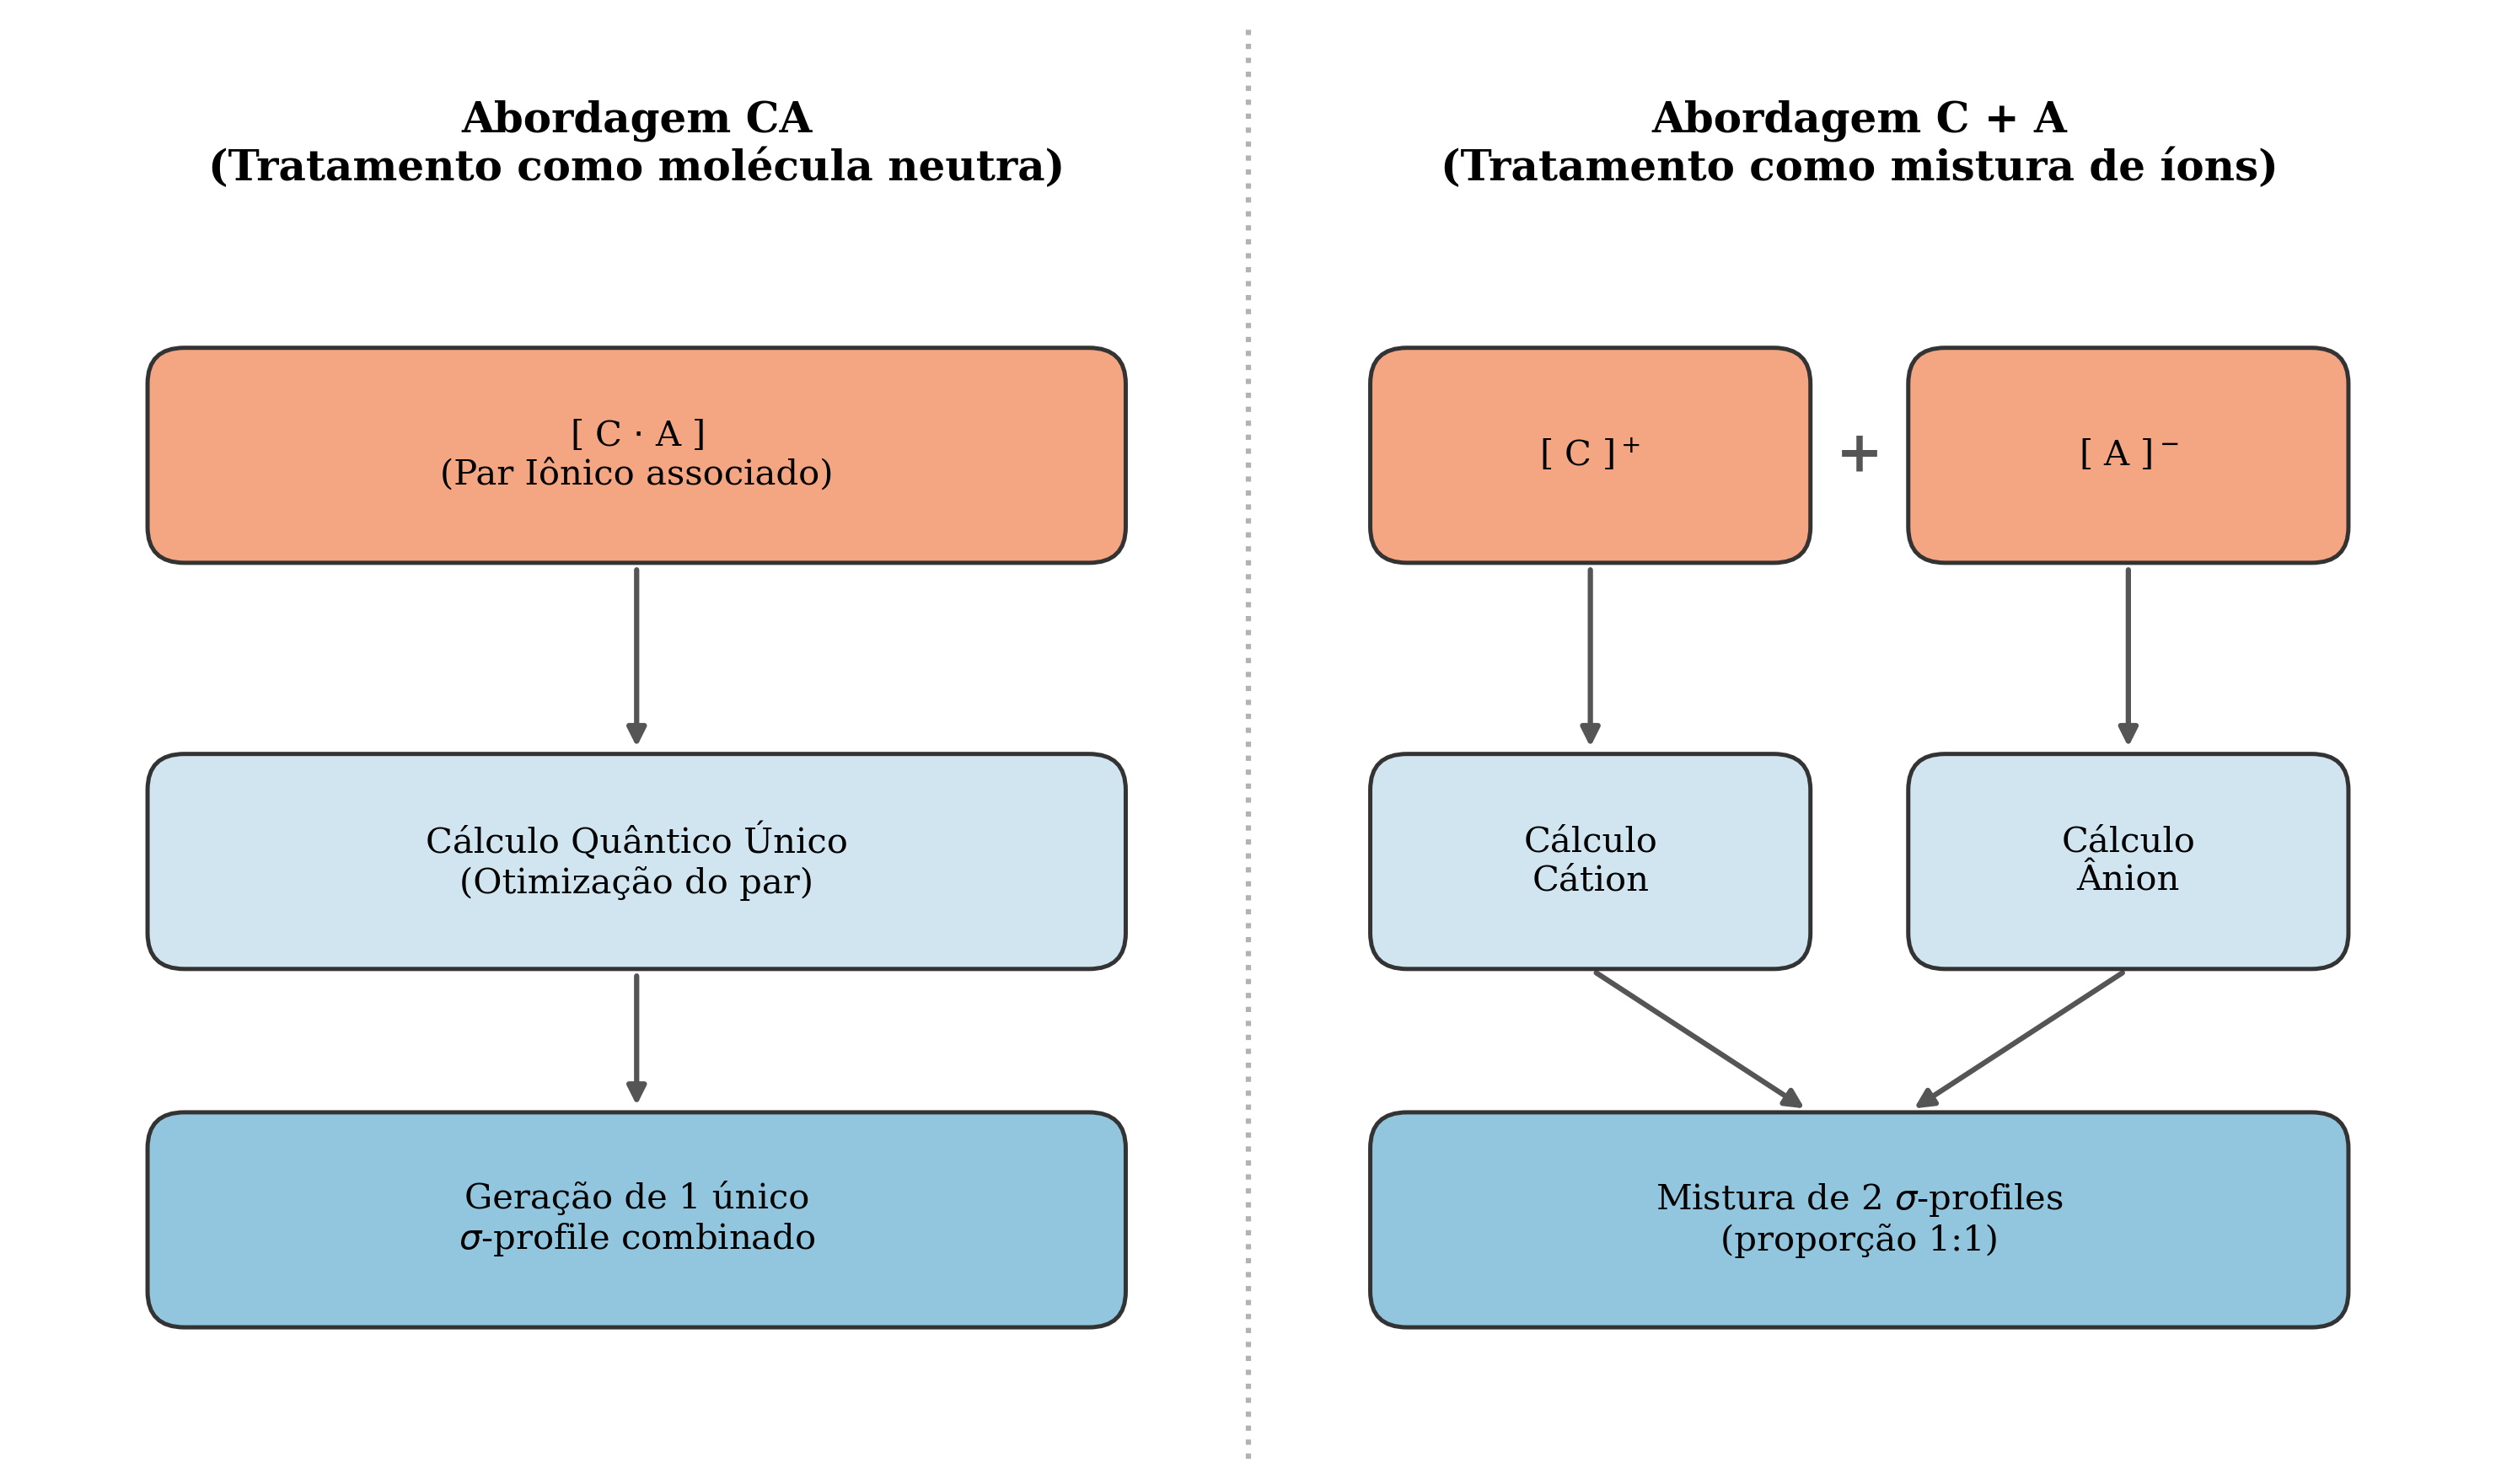
\includegraphics[width=0.7\linewidth]{imagens/fig3_esquema_CA.png}
    \caption{Comparação esquemática entre as abordagens CA (par iônico neutro) e C+A (íons separados), ilustrando a construção dos $\sigma$-profiles em cada caso.}
    \label{fig:CA_C+A}
\end{figure}

Esse precedente da literatura motivou a avaliação inicial da abordagem C+A para os líquidos iônicos próticos deste trabalho. Os cálculos COSMO foram realizados separadamente para os cátions [2-HEA]$^+$ e [DETA]$^+$ e para o ânion hexanoato [Hx]$^-$, e os $\sigma$-profiles combinados conforme a Equação~\ref{eq:sigma_profile_ca}. Essa avaliação, no entanto, revelou uma limitação prática severa: os coeficientes de atividade em diluição infinita calculados a partir dos íons separados assumiram valores fisicamente implausíveis, da ordem de $10^{11}$ a $10^{15}$, muito acima do que se observa para qualquer par soluto-solvente real. Esse resultado indica que, ao separar cátion e ânion em cavidades COSMO independentes, o modelo perde a compensação eletrostática que naturalmente ocorre entre as duas espécies quando associadas, superestimando de forma acentuada a energia de restauração de cada íon isolado.

Diante dessa limitação, adotou-se neste trabalho a abordagem CA (par iônico neutro) para os líquidos iônicos próticos [2-HEA][Hx] e [DETA][Hx] no COSMO-SAC, na mesma linha da estratégia já adotada para o UNIFAC-LL (Seção~\ref{sec:unifacll}). O cálculo COSMO é realizado sobre o par cátion-ânion como uma única entidade neutra, o que produziu coeficientes de atividade com magnitude fisicamente coerente e consistente com o comportamento esperado para líquidos iônicos em solução. Essa escolha diverge do precedente estabelecido por \citeonline{dominguez2014} e \citeonline{xu2022} para líquidos iônicos de imidazólio, o que sugere que a superioridade relativa entre as duas abordagens pode depender da estrutura específica do líquido iônico em questão, e não constitui uma regra geral aplicável a qualquer combinação cátion-ânion. Os detalhes do nível de teoria empregado nos cálculos COSMO de cada par iônico são apresentados no Capítulo~\ref{cap:metodologia}.

\section{O modelo UNIFAC-LL}
\label{sec:unifacll}

O UNIFAC (\textit{UNIversal quasichemical Functional group Activity Coefficients}), proposto por \citeonline{fredenslund1975}, é um modelo de coeficiente de atividade baseado no conceito de contribuição por grupos funcionais. A premissa central é que uma molécula pode ser representada como um conjunto de grupos estruturais (por exemplo, \ce{CH3}, \ce{CH2}, \ce{OH}, \ce{COOH}, \ce{NH2}), e que as interações intermoleculares na mistura podem ser aproximadas pelas interações entre esses grupos, independentemente da molécula à qual pertencem\cite{fredenslund1975}. A variante UNIFAC-LL, parametrizada por \citeonline{magnussen1981} especificamente para a predição de equilíbrio líquido-líquido, é a versão empregada no Capítulo\ref{cap:resultados} deste trabalho como referência comparativa ao COSMO-SAC.

% -----------------------------------------------------------------
% Estrutura do coeficiente de atividade
% -----------------------------------------------------------------

Assim como no COSMO-SAC, o coeficiente de atividade no UNIFAC é expresso como a soma de uma contribuição combinatorial e uma contribuição residual\cite{fredenslund1975}:

\begin{equation}
    \ln \gamma_i = \ln \gamma_i^{comb} + \ln \gamma_i^{res}
    \label{eq:gamma_unifac}
\end{equation}

A contribuição combinatorial é calculada pelo mesmo modelo de Staverman-Guggenheim apresentado na Equação\ref{eq:gamma_combinatorial}, com a diferença de que os parâmetros de volume ($R_k$) e área superficial ($Q_k$) de cada grupo funcional são valores tabelados, obtidos a partir de dados de van der Waals, e não da cavidade COSMO\cite{fredenslund1975}. O volume e a área normalizados de cada molécula são calculados como a soma das contribuições de todos os grupos que a compõem:

\begin{equation}
    r_i = \sum_{k} \nu_k^{(i)} R_k \qquad \text{e} \qquad
    q_i = \sum_{k} \nu_k^{(i)} Q_k
    \label{eq:rq_unifac}
\end{equation}

\noindent em que $\nu_k^{(i)}$ é o número de grupos do tipo $k$ na molécula $i$, e $R_k$ e $Q_k$ são os parâmetros de volume e área do grupo $k$.

% -----------------------------------------------------------------
% Contribuição residual
% -----------------------------------------------------------------

A contribuição residual, por outro lado, difere fundamentalmente da abordagem COSMO-SAC. No UNIFAC, ela é calculada a partir das interações entre pares de grupos funcionais, e não entre segmentos de superfície\cite{fredenslund1975}:

\begin{equation}
    \ln \gamma_i^{res} = \sum_{k} \nu_k^{(i)}
    \left[ \ln \Gamma_k - \ln \Gamma_k^{(i)} \right]
    \label{eq:gamma_res_unifac}
\end{equation}

\noindent em que $\Gamma_k$ é o coeficiente de atividade do grupo $k$ na mistura e $\Gamma_k^{(i)}$ é o coeficiente de atividade do mesmo grupo em uma solução de referência contendo apenas moléculas do tipo $i$. O coeficiente de atividade de grupo é dado por\cite{fredenslund1975}:

\begin{equation}
    \ln \Gamma_k = Q_k \left[
    1 - \ln\!\left(\sum_{m} \Theta_m \Psi_{mk}\right)
    - \sum_{m} \frac{\Theta_m \Psi_{km}}
                    {\displaystyle\sum_{n} \Theta_n \Psi_{nm}}
    \right]
    \label{eq:gamma_grupo}
\end{equation}

\noindent em que $\Theta_m$ é a fração de área superficial do grupo $m$ na mistura e $\Psi_{mn}$ é o parâmetro de interação entre os grupos $m$ e $n$, definido como:

\begin{equation}
    \Psi_{mn} = \exp\!\left(-\frac{a_{mn}}{T}\right)
    \label{eq:psi_unifac}
\end{equation}

Os parâmetros $a_{mn}$ (em unidades de Kelvin) são os parâmetros de interação binários entre grupos, e constituem o elemento central da capacidade preditiva do modelo. Eles são determinados por regressão a partir de dados experimentais de equilíbrio de fases de sistemas conhecidos e organizados em uma matriz de parâmetros de interação, na qual cada entrada corresponde a um par de grupos funcionais\cite{magnussen1981}. Uma vez disponíveis, esses parâmetros permitem predizer o comportamento de qualquer mistura cujas moléculas sejam decomponíveis nos grupos tabelados. A parametrização de \citeonline{magnussen1981} para ELL (UNIFAC-LL) abrange um conjunto de grupos especificamente ajustado à descrição de sistemas com duas fases líquidas, com parâmetros de interação distintos daqueles utilizados nas versões do UNIFAC para equilíbrio líquido-vapor.

% -----------------------------------------------------------------
% Limitações para líquidos iônicos
% -----------------------------------------------------------------

A natureza preditiva do UNIFAC-LL está, portanto, condicionada à disponibilidade de parâmetros de interação para todos os pares de grupos presentes no sistema de interesse. Essa condição impõe uma limitação estrutural quando o modelo é aplicado a sistemas contendo líquidos iônicos. Os cátions e ânions dos LIs podem, em princípio, ser decompostos em grupos funcionais existentes na tabela UNIFAC (por exemplo, \ce{CH2}, \ce{OH}, \ce{NH2}, \ce{COOH}). No entanto, a matriz de Magnussen não contém parâmetros de interação para diversos pares de grupos que surgem quando os grupos representativos dos LIs interagem entre si ou com os demais componentes do sistema\cite{bahadur2015}.

No caso específico dos sistemas estudados neste trabalho, a decomposição dos LIPs [2-HEA][Hx] e [DETA][Hx] em grupos UNIFAC gera pares de interação para os quais os parâmetros $a_{mn}$ são inexistentes na parametrização de Magnussen, como os pares envolvendo grupos \ce{CNH2}/\ce{CCOO} e \ce{CCOO}/\ce{CNH2}. Sem esses parâmetros, o cálculo dos coeficientes de atividade das espécies iônicas seria inviável, o que exige o preenchimento dessa lacuna por meio de um modelo preditivo de aprendizado de máquina, conforme detalhado no Capítulo~\ref{cap:metodologia}. Essa lacuna não é de implementação, mas sim estrutural: decorre do fato de que a matriz de parâmetros foi construída a partir de dados experimentais de sistemas orgânicos convencionais, nos quais líquidos iônicos não estavam presentes\cite{bahadur2015,magnussen1981}, e sua resolução via aprendizado de máquina, em vez de calibração direta, é retomada na discussão das limitações do modelo (Capítulo~\ref{cap:resultados}).

\begin{figure}[H]
    \centering
    \resizebox{\textwidth}{!}{%
    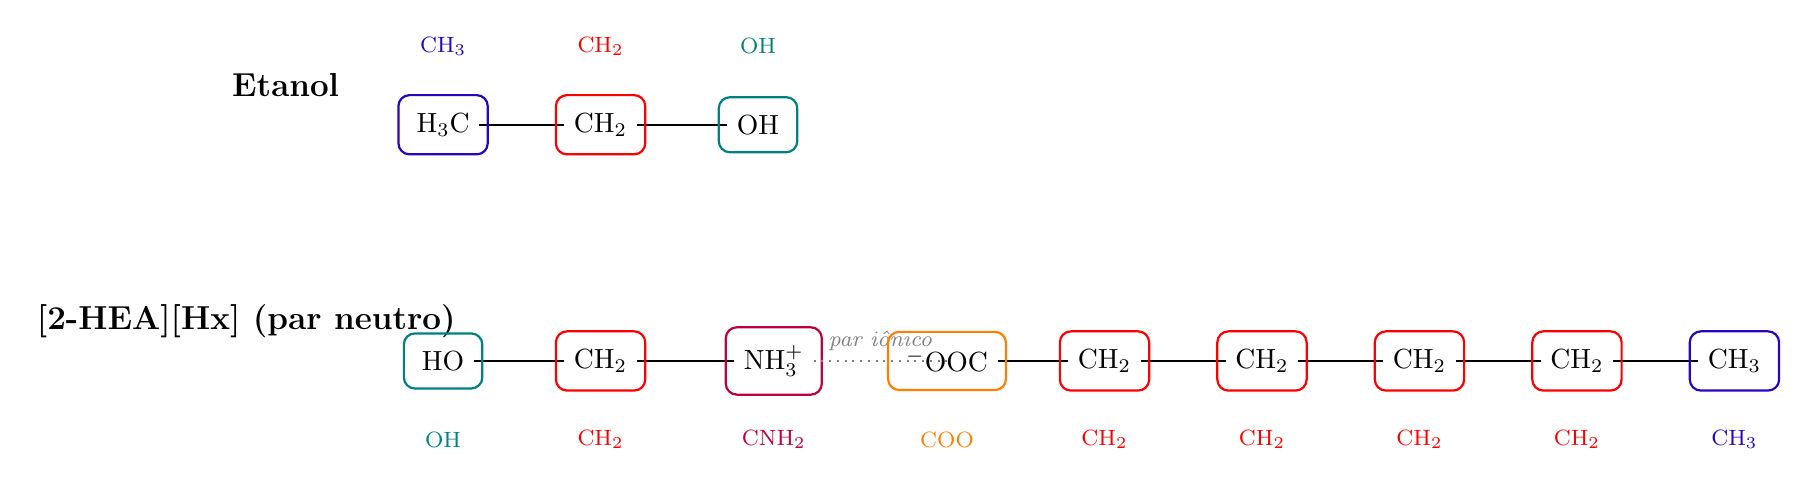
\begin{tikzpicture}[
        group/.style={thick, rounded corners, inner sep=3pt},
        label/.style={font=\footnotesize}
    ]
    
    % ── ETANOL ───────────────────────────────────
    \node[font=\large] at (-2, 5.5) {\textbf{Etanol}};
    
    \node (ch3) at (0, 5) {H$_3$C};
    \node (ch2) at (2, 5) {CH$_2$};
    \node (oh)  at (4, 5) {OH};
    
    \draw[thick] (ch3) -- (ch2) -- (oh);
    
    \node[draw=blue, group, fit=(ch3)] {};
    \node[draw=red, group, fit=(ch2)] {};
    \node[draw=teal, group, fit=(oh)] {};
    
    \node[blue, label] at (0, 6.0) {CH$_3$};
    \node[red, label]  at (2, 6.0) {CH$_2$};
    \node[teal, label] at (4, 6.0) {OH};
    
    % ── [2-HEA][Hx]: PAR IÔNICO NEUTRO COMPLETO ──
    \node[font=\large] at (-2.5, 2.5) {\textbf{[2-HEA][Hx] (par neutro)}};
    
    % Cátion [2-HEA]+
    \node (oh2)  at (0, 2) {HO};
    \node (c2a)  at (2, 2) {CH$_2$};
    \node (nh3)  at (4.2, 2) {NH$_3^+$};
    
    \draw[thick] (oh2) -- (c2a) -- (nh3);
    
    \node[draw=teal, group, fit=(oh2)] {};
    \node[draw=red, group, fit=(c2a)] {};
    \node[draw=purple, group, fit=(nh3)] {};
    
    \node[teal, label]   at (0, 1.0) {OH};
    \node[red, label]    at (2, 1.0) {CH$_2$};
    \node[purple, label] at (4.2, 1.0) {CNH$_2$};
    
    % Interação iônica (par neutro)
    \draw[thick, dotted, gray] (nh3) -- (6.4, 2)
        node[midway, above, font=\footnotesize\itshape, gray] {par iônico};
    
    % Ânion [Hx]- (carboxilato: grupo COO, distinto do éster CCOO dos triglicerídeos)
    \node (coo)  at (6.4, 2) {$^{-}$OOC};
    \node (c3a)  at (8.4, 2) {CH$_2$};
    \node (c3b)  at (10.4, 2) {CH$_2$};
    \node (c3c)  at (12.4, 2) {CH$_2$};
    \node (c3d)  at (14.4, 2) {CH$_2$};
    \node (ch3b) at (16.4, 2) {CH$_3$};
    
    \draw[thick] (coo) -- (c3a) -- (c3b) -- (c3c) -- (c3d) -- (ch3b);
    
    \node[draw=orange, group, fit=(coo)] {};
    \node[draw=red, group, fit=(c3a)] {};
    \node[draw=red, group, fit=(c3b)] {};
    \node[draw=red, group, fit=(c3c)] {};
    \node[draw=red, group, fit=(c3d)] {};
    \node[draw=blue, group, fit=(ch3b)] {};
    
    \node[orange, label] at (6.4, 1.0)  {COO};
    \node[red, label]    at (8.4, 1.0)  {CH$_2$};
    \node[red, label]    at (10.4, 1.0) {CH$_2$};
    \node[red, label]    at (12.4, 1.0) {CH$_2$};
    \node[red, label]    at (14.4, 1.0) {CH$_2$};
    \node[blue, label]   at (16.4, 1.0) {CH$_3$};
    
    \end{tikzpicture}%
    }
    
    \caption{Decomposição em grupos UNIFAC para o etanol
    (1 CH$_3$ + 1 CH$_2$ + 1 OH) e para o par iônico neutro [2-HEA][Hx]
    (cátion: 1 OH + 1 CH$_2$ + 1 CNH$_2$; ânion: 1 COO + 4 CH$_2$ + 1 CH$_3$),
    tratado como uma única espécie neutra pelo modelo. O grupo COO(41)
    do carboxilato aniônico é distinto do grupo éster CCOO(11) presente
    nos triglicerídeos (Tabela~\ref{tab:decomposicao_unifac}), refletindo
    o diferente ambiente químico de cada ligação carbono-oxigênio.}
    \label{fig:unifac_decomposition}
\end{figure}

É essa limitação paramétrica, contrastada com a natureza a priori do COSMO-SAC discutida na Seção~\ref{subsec:cosmo_parametros}, que motiva a comparação sistemática entre os dois modelos neste trabalho, conforme discutido na introdução (Capítulo \ref{introducao}).

\begin{longtable}{p{3.2cm}p{5.4cm}p{5.4cm}}
\caption{Comparação entre os modelos UNIFAC-LL e COSMO-SAC.}
\label{tab:comparacao_modelos} \\
\toprule
\textbf{Característica} & \textbf{UNIFAC-LL} & \textbf{COSMO-SAC} \\
\midrule
\endfirsthead

\multicolumn{3}{c}{\tablename\ \thetable\ -- continuação} \\
\toprule
\textbf{Característica} & \textbf{UNIFAC-LL} & \textbf{COSMO-SAC} \\
\midrule
\endhead

\bottomrule
\endfoot

Natureza preditiva & Empírico, baseado em contribuição de grupos funcionais (FREDENSLUND; JONES; PRAUSNITZ, 1975) & A priori, baseado em propriedades moleculares calculadas por química quântica (LIN; SANDLER, 2002) \\
\addlinespace
Parâmetros necessários & Parâmetros de interação binários entre grupos ($a_{mn}$), ajustados a dados experimentais de mistura (MAGNUSSEN; RASMUSSEN; FREDENSLUND, 1981) & Parâmetros universais ($a_{eff}$, $r_{eff}$, $f_{pol}$, $c_{hb}$, $\sigma_{hb}$, $r_{std}$, $q_{std}$), calibrados uma única vez e válidos para qualquer sistema (LIN; SANDLER, 2002) \\
\addlinespace
Origem da informação molecular & Decomposição da molécula em grupos funcionais tabelados & $\sigma$-profile obtido por cálculo DFT/COSMO da molécula isolada \\
\addlinespace
Contribuição residual & Interação entre pares de grupos funcionais ($\Psi_{mn}$) & Interação entre segmentos de superfície ($\Delta W(\sigma_m,\sigma_n)$) \\
\addlinespace
Tratamento de líquidos iônicos & Lacuna paramétrica original preenchida por modelo de ML (HAYER et al., 2025), já que a matriz de Magnussen carece de pares como CNH2/CCOO (BAHADUR et al., 2015); adota-se o par iônico neutro & Abordagem C+A avaliada e descartada por gerar $\gamma^\infty$ fisicamente implausível ($10^{11}$--$10^{15}$); adota-se o par iônico neutro (mesma estratégia do UNIFAC-LL) \\
\addlinespace
Dependência de dados experimentais da mistura & Sim, para o ajuste dos parâmetros binários & Não, apenas para validação posterior do modelo \\

\end{longtable}
\chapter{Metodologia}
\label{cap:metodologia}

\epigraph{\textit{"A simplicidade é o último grau de sofisticação."}}{\textbf{--- Leonardo da Vinci}}

\section{Definição dos sistemas e condições de estudo}
\label{sec:sistemas}

O presente trabalho investiga o equilíbrio líquido-líquido de sistemas ternários do tipo \{triglicerídeo + álcool + líquido iônico prótico\}, combinando três triglicerídeos, dois álcoois e dois líquidos iônicos próticos (LIPs), o que totaliza doze sistemas ternários distintos, cada um avaliado pelos dois modelos termodinâmicos (UNIFAC-LL e COSMO-SAC). Todos os sistemas são estudados a 298,15~K e pressão atmosférica.

Os triglicerídeos estudados são a trioleína (\ce{C57H104O6}), a trilinoleína (\ce{C57H98O6}) e a trilinolenina (\ce{C57H92O6}), formadas respectivamente por três cadeias de ácido oleico (uma insaturação por cadeia), ácido linoleico (duas insaturações) e ácido linolênico (três insaturações). Essa escolha permite avaliar sistematicamente o efeito do grau de insaturação da cadeia graxa sobre a miscibilidade do sistema, mantendo fixo o número de carbonos por cadeia (C18) e variando apenas o número de ligações duplas.

Os álcoois estudados são o etanol e o metanol, o que permite avaliar o efeito da cadeia alquílica do álcool (dois carbonos contra um) sobre a extensão e a posição da região bifásica, além de permitir a comparação direta com os estudos experimentais de \citeonline{trindade2019} e \citeonline{gomez2019}, que empregam metanol.

Os líquidos iônicos próticos estudados são o hexanoato de 2-hidroxietilamônio ([2-HEA][Hx]) e o hexanoato de dietilenotriamônio ([DETA][Hx]), cuja escolha se fundamenta nos resultados experimentais de \citeonline{gomez2019} e \citeonline{trindade2019}, respectivamente, que demonstraram a eficácia desses dois LIPs como cossolventes na transesterificação alcalina de óleo de soja. Os dois LIPs compartilham o mesmo ânion (hexanoato) e diferem na estrutura do cátion: o [2-HEA]$^+$ possui um grupo hidroxila na cadeia lateral e uma única carga positiva, enquanto o [DETA]$^{+3}$ apresenta uma cadeia aminada estendida, triprotonada, com maior capacidade de doação e aceitação de ligações de hidrogênio. Essa variação estrutural controlada (mesmo ânion, cátions distintos) permite isolar o efeito da estrutura do cátion sobre a miscibilidade do sistema, o que constitui um dos eixos centrais da análise comparativa proposta nos objetivos deste trabalho.

A trioleína é adotada como o sistema central de análise ao longo deste trabalho, por ser o principal triglicerídeo presente no óleo de soja, matéria-prima empregada nos estudos experimentais de referência \cite{trindade2019,gomez2019}. A utilização de triglicerídeos puros como \textit{surrogates}, em vez de um óleo vegetal real (que contém dezenas de triglicerídeos com diferentes perfis de ácidos graxos), é prática consolidada na literatura de modelagem termodinâmica de sistemas de biodiesel, pois permite representar o comportamento da fase oleosa sem a complexidade composicional de uma mistura real \cite{ferrarini2018}. A trilinoleína e a trilinolenina são incluídas como variações controladas da trioleína, isolando o efeito do grau de insaturação sobre os resultados obtidos para o sistema central.

\begin{figure}[H]
\caption{Fluxograma geral do pipeline metodológico, mostrando os dois caminhos
paralelos de cálculo do equilíbrio líquido-líquido.}
\label{fig:fluxograma_pipeline}
\centering
\resizebox{\textwidth}{!}{%
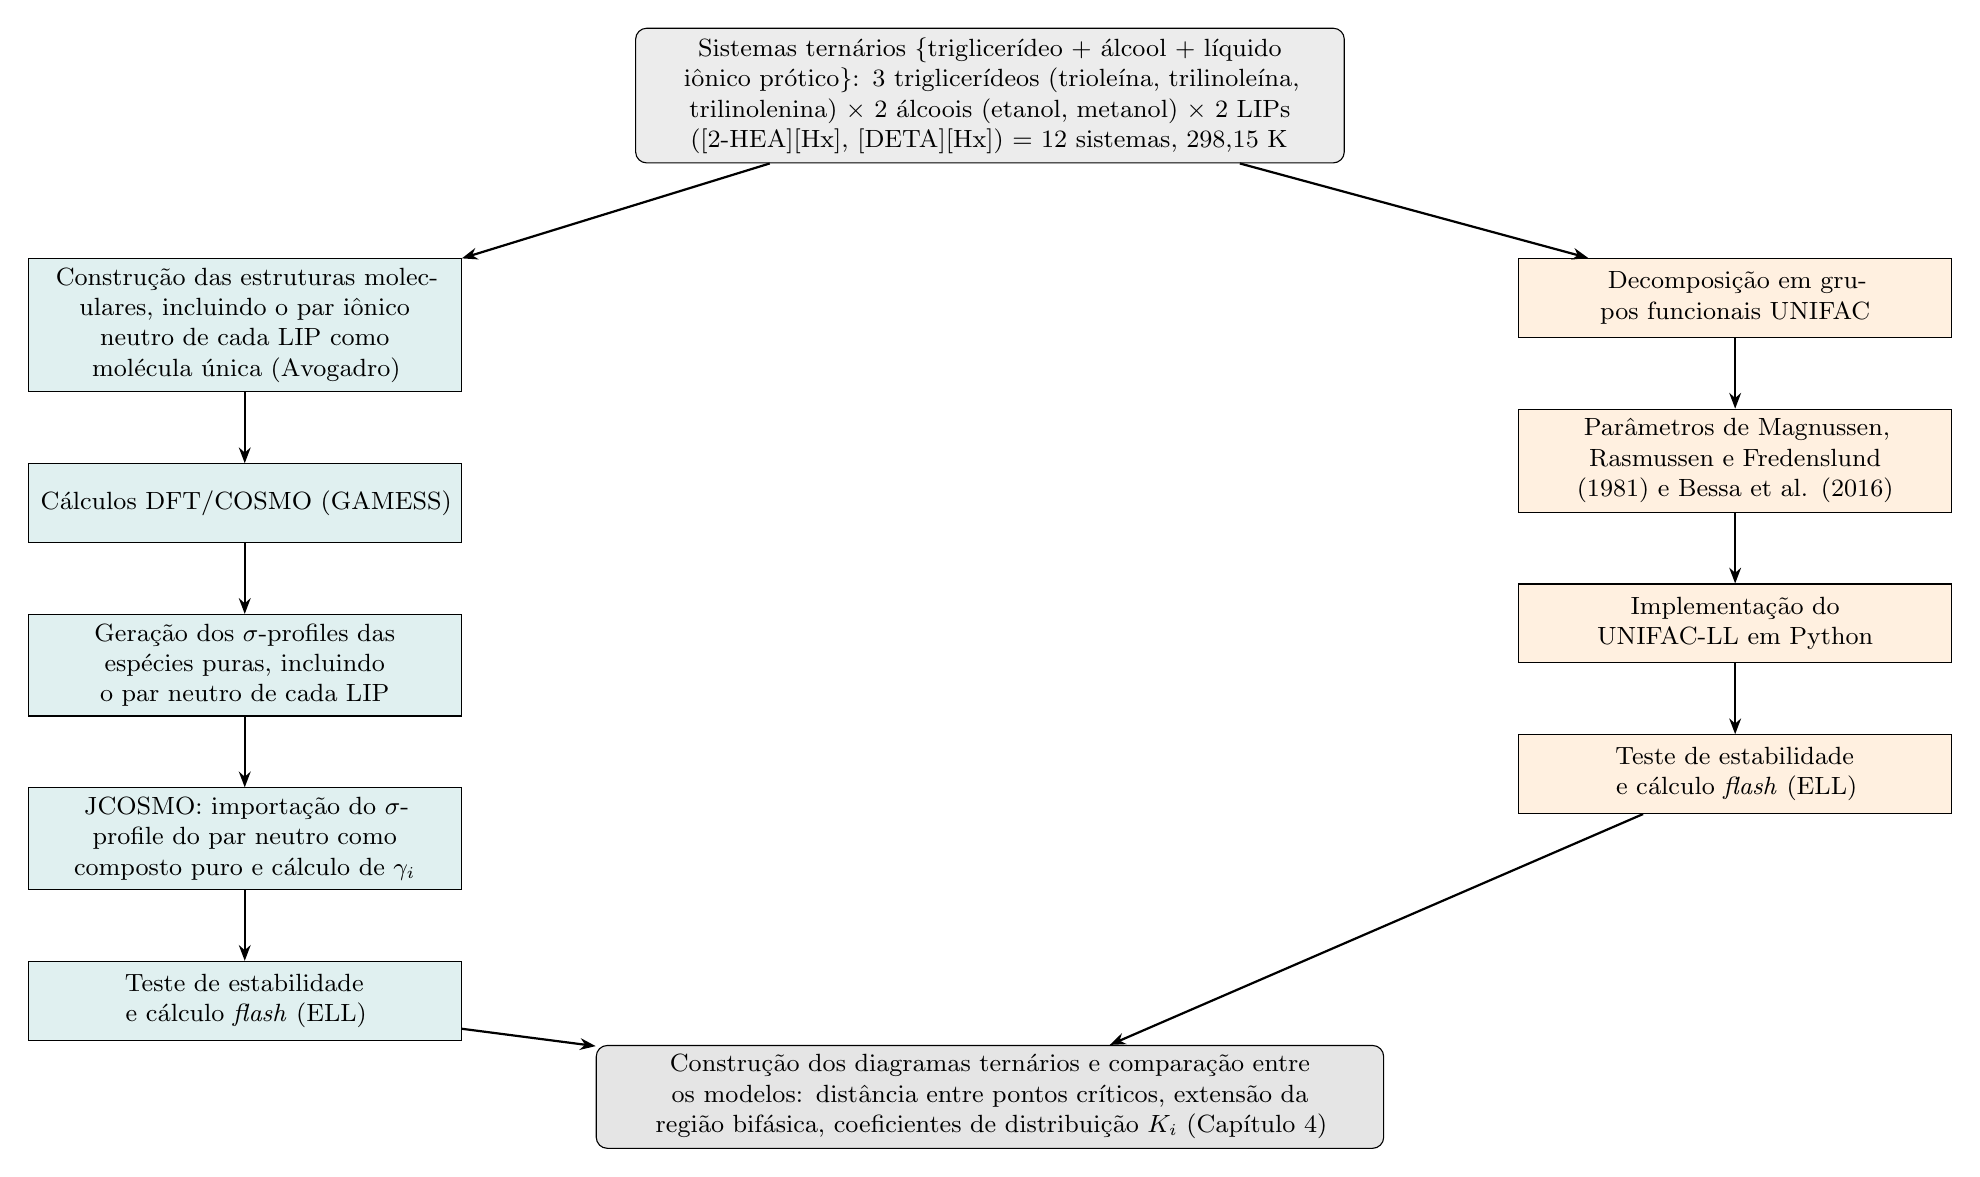
\begin{tikzpicture}[node distance=0.9cm and 1cm]

\tikzstyle{topo} = [rectangle, rounded corners, minimum width=9cm, minimum height=1cm,
    text width=8.5cm, align=center, draw=black, fill=gray!15, font=\small]
\tikzstyle{cosmo} = [rectangle, minimum width=5.5cm, minimum height=1cm,
    text width=5.2cm, align=center, draw=black, fill=teal!12, font=\small]
\tikzstyle{unifac} = [rectangle, minimum width=5.5cm, minimum height=1cm,
    text width=5.2cm, align=center, draw=black, fill=orange!12, font=\small]
\tikzstyle{merge} = [rectangle, rounded corners, minimum width=10cm, minimum height=1.1cm,
    text width=9.5cm, align=center, draw=black, fill=gray!20, font=\small]
\tikzstyle{seta} = [thick, -{Stealth[length=2mm]}]

\node (sistemas) [topo] {Sistemas ternários \{triglicerídeo + álcool + líquido iônico prótico\}: 3 triglicerídeos (trioleína, trilinoleína, trilinolenina) $\times$ 2 álcoois (etanol, metanol) $\times$ 2 LIPs ([2-HEA][Hx], [DETA][Hx]) = 12 sistemas, 298,15~K};

% coluna COSMO-SAC
\node (avogadro) [cosmo, below left=1.2cm and 2.2cm of sistemas]
    {Construção das estruturas moleculares, incluindo o par iônico neutro de cada LIP como molécula única (Avogadro)};
\node (gamess) [cosmo, below=of avogadro] {Cálculos DFT/COSMO (GAMESS)};
\node (sigmaprofiles) [cosmo, below=of gamess]
    {Geração dos $\sigma$-profiles das espécies puras, incluindo o par neutro de cada LIP};
\node (jcosmo) [cosmo, below=of sigmaprofiles]
    {JCOSMO: importação do $\sigma$-profile do par neutro como composto puro e cálculo de $\gamma_i$};
\node (ellcosmo) [cosmo, below=of jcosmo]
    {Teste de estabilidade e cálculo \textit{flash} (ELL)};

% coluna UNIFAC-LL
\node (decomp) [unifac, below right=1.2cm and 2.2cm of sistemas]
    {Decomposição em grupos funcionais UNIFAC};
\node (parametros) [unifac, below=of decomp]
    {Parâmetros de Magnussen, Rasmussen e Fredenslund (1981) e Bessa et al. (2016)};
\node (python) [unifac, below=of parametros]
    {Implementação do UNIFAC-LL em Python};
\node (ellunifac) [unifac, below=of python]
    {Teste de estabilidade e cálculo \textit{flash} (ELL)};

% nó final
\node (comparacao) [merge, below=2.0cm of $(ellcosmo)!0.5!(ellunifac)$]
    {Construção dos diagramas ternários e comparação entre os modelos: distância
    entre pontos críticos, extensão da região bifásica, coeficientes de
    distribuição $K_i$ (Capítulo 4)};

% setas
\draw [seta] (sistemas) -- (avogadro);
\draw [seta] (sistemas) -- (decomp);
\draw [seta] (avogadro) -- (gamess);
\draw [seta] (gamess) -- (sigmaprofiles);
\draw [seta] (sigmaprofiles) -- (jcosmo);
\draw [seta] (jcosmo) -- (ellcosmo);
\draw [seta] (decomp) -- (parametros);
\draw [seta] (parametros) -- (python);
\draw [seta] (python) -- (ellunifac);
\draw [seta] (ellcosmo) -- (comparacao);
\draw [seta] (ellunifac) -- (comparacao);

\end{tikzpicture}%
}
\end{figure}

Cabe uma ressalva sobre a temperatura de trabalho adotada. Os ganhos de rendimento atribuídos ao efeito cossolvente dos líquidos iônicos próticos, reportados por \citeonline{trindade2019} e \citeonline{gomez2019} e que motivam este trabalho, foram obtidos em condição reacional, a aproximadamente 60\,°C. O equilíbrio líquido-líquido modelado neste trabalho, a 298,15~K, não representa diretamente essa condição reacional, mas sim uma etapa distinta e também relevante do processo: a separação de fases do meio reacional após o resfriamento, etapa que antecede a purificação do biodiesel e que tipicamente ocorre próxima à temperatura ambiente. A cossolvência observada experimentalmente por Trindade e Gomez é, portanto, um fenômeno à temperatura de reação, enquanto os diagramas de ELL apresentados neste trabalho caracterizam o comportamento de fases numa condição posterior e distinta, ainda que igualmente relevante para o desempenho global do processo. Essa distinção é retomada na interpretação dos resultados (Seção~\ref{subsec:salting_in_out}), e a extensão dos resultados aqui apresentados para a condição reacional a 60\,°C permanece como uma limitação de escopo deste trabalho, não coberta pelos sistemas modelados.

\section{Dados experimentais para validação}
\label{sec:dados_validacao}

A avaliação da capacidade preditiva de um modelo termodinâmico requer a comparação entre os resultados simulados e dados experimentais de equilíbrio de fases. No caso do presente trabalho, essa comparação enfrenta uma limitação importante: a revisão bibliográfica conduzida não identificou dados experimentais publicados de equilíbrio líquido-líquido (composições das fases coexistentes, linhas de amarração) para os doze sistemas ternários \{triglicerídeo + álcool + líquido iônico prótico\} estudados neste trabalho. Os trabalhos de \citeonline{trindade2019} e \citeonline{gomez2019}, que constituem a motivação experimental deste estudo, reportam dados de rendimento mássico de biodiesel em função da concentração de cossolvente, mas não incluem a determinação das composições das fases em equilíbrio no sistema ternário.

Diante dessa limitação, a estratégia de validação adotada neste trabalho é dividida em duas etapas. A primeira consiste na validação metodológica do modelo COSMO-SAC em sistemas ternários análogos para os quais dados experimentais de ELL estão disponíveis na literatura.
\citeonline{xu2022} publicaram dados de ELL para sistemas do tipo \{éster + álcool + LI de imidazólio\} a 298,15 K, incluindo linhas de amarração e curvas binodais. Esses sistemas compartilham com os sistemas-alvo a presença simultânea de um éster, um álcool e um líquido iônico, o que os torna representativos para avaliar se o COSMO-SAC captura adequadamente as interações intermoleculares relevantes nessa classe de misturas. \citeonline{dominguez2014} fornecem dados de ELL para sistemas \{hidrocarboneto alifático + hidrocarboneto aromático + LI de imidazólio\} a 298,15 K, que permitem avaliar o desempenho do modelo na descrição de sistemas com líquidos iônicos em geral. Esses dois conjuntos de dados foram identificados como sistemas de referência adequados para essa validação externa; sua aplicação efetiva, contudo, limitou-se neste trabalho a uma verificação qualitativa da qualidade geométrica dos perfis sigma envolvidos (Seção~\ref{subsec:parametros_perfis}), sem uma quantificação por RMSD equivalente à realizada para o UNIFAC-LL. Essa lacuna é registrada como limitação na Seção~\ref{subsec:sintese} e na Conclusão, e sua resolução é sugerida como direção de trabalho futuro.

A segunda etapa consiste na análise dos diagramas ternários simulados para os próprios sistemas-alvo, na ausência de dados experimentais diretos. Nesse caso, a avaliação é de natureza qualitativa e apoia-se na comparação entre o comportamento previsto pelos modelos e as observações experimentais indiretas reportadas por \citeonline{trindade2019} e \citeonline{gomez2019}. Examina-se, para cada sistema, em que sentido a adição do líquido iônico prótico altera a extensão da região bifásica, e confronta-se o resultado com os ganhos de rendimento relatados por esses autores, atentando para as diferenças de temperatura, de faixa de concentração e de natureza da grandeza medida que separam as duas situações. A comparação entre os dois líquidos iônicos ([2-HEA][Hx] e [DETA][Hx]) é conduzida da mesma forma, sem que se assuma, de antemão, qual direção o resultado computacional deve tomar.

Para a validação da implementação do UNIFAC-LL, descrita na Seção \ref{sec:unifac_implementacao}, emprega-se o sistema ternário \{n-hexano + etanol + água\}, para o qual dados experimentais de ELL estão amplamente disponíveis na literatura e a parametrização de \citeonline{magnussen1981} é completa. Esse sistema serve exclusivamente como verificação da corretude da implementação computacional, e não como avaliação da capacidade do UNIFAC-LL de descrever sistemas contendo líquidos iônicos.

\section{Construção das estruturas moleculares}
\label{sec:estruturas}

As estruturas moleculares tridimensionais das nove espécies neutras envolvidas nos cálculos COSMO foram construídas no \textit{software} Avogadro (\textit{open-source}), um editor molecular que permite a construção, visualização e edição de geometrias moleculares em três dimensões \cite{avogadro2012}. As espécies modeladas são: etanol (\ce{C2H6O}), metanol (\ce{CH4O}), trioleína (\ce{C57H104O6}), trilinoleína (\ce{C57H98O6}), trilinolenina (\ce{C57H92O6}), ácido oleico (\ce{C18H34O2}), ácido linoleico (\ce{C18H32O2}) e os pares iônicos neutros [2-HEA][Hx] e [DETA][Hx]. Dessas nove, apenas os dois pares iônicos neutros foram efetivamente submetidos a cálculo DFT/COSMO no GAMESS pela autora deste trabalho (Seção~\ref{sec:dft_cosmo}); as demais sete espécies, construídas no Avogadro como parte da modelagem inicial do sistema, tiveram seus $\sigma$-profiles finais obtidos diretamente do banco de dados interno do JCOSMO (Tabela~\ref{tab:cosmo_detalhes}), já calculados e validados pelo desenvolvedor da ferramenta, de modo que a construção dessas sete no Avogadro serviu à modelagem preliminar e à conferência estrutural, mas não alimentou diretamente nenhum cálculo de química quântica realizado neste trabalho.

Para os três triglicerídeos, a geometria inicial foi obtida a partir do banco de dados interno do Avogadro, que fornece estruturas pré-construídas para diversas moléculas de interesse. Os três compartilham o mesmo núcleo de glicerol esterificado a três cadeias de ácido graxo C18, diferindo apenas no grau de insaturação de cada cadeia (uma, duas e três ligações duplas, respectivamente, para trioleína, trilinoleína e trilinolenina). A trioleína constitui o principal componente do óleo de soja, matéria-prima empregada nos estudos experimentais de referência \cite{trindade2019,gomez2019}, e é adotada como sistema central de análise (Seção~\ref{sec:sistemas}). Cada triglicerídeo possui em torno de 160 a 170 átomos, o que os torna significativamente maiores do que as demais espécies do sistema.

Os ácidos oleico e linoleico, empregados na avaliação dos sistemas com ácido graxo livre (Seção~\ref{subsec:casos_sem_separacao}), tiveram suas geometrias iniciais obtidas da mesma forma, a partir do banco de dados interno do Avogadro, e compartilham com a trioleína e a trilinoleína, respectivamente, a mesma cadeia graxa C18 com o mesmo grau de insaturação, diferindo apenas pela ausência do núcleo de glicerol e das demais duas cadeias esterificadas.

Para os líquidos iônicos próticos, conforme a estratégia de par iônico neutro adotada (Seção~\ref{sec:cosmo_li}), o cátion e o ânion de cada LIP foram construídos no Avogadro e, em seguida, efetivamente otimizados por cálculo quântico no GAMESS, integrado ao cálculo COSMO, sem etapa prévia de pré-otimização por campo de forças, como uma única molécula neutra, e não como espécies carregadas independentes. O par [2-HEA][Hx] foi montado unindo o cátion 2-hidroxietilamônio (produto da protonação da monoetanolamina, com um grupo amônio \ce{-NH3+} e um grupo hidroxila \ce{-OH} na cadeia lateral) ao ânion hexanoato, por meio de uma ligação iônica N-H$\cdots$O entre o hidrogênio ácido do grupo amônio e um dos oxigênios do carboxilato. O par [DETA][Hx] foi montado de forma análoga, unindo o cátion dietilenotriamônio triprotonado (produto da triprotonação da dietilenotriamina, com três átomos de nitrogênio protonados na cadeia) a três ânions hexanoato, um para cada sítio protonado, na estequiometria 1:3 confirmada experimentalmente por \citeonline{trindade2019}, que reporta a síntese do [DETA][Hx] a partir de 1 mol de dietilenotriamina e 3 mol de ácido hexanoico. As geometrias dos dois pares foram ajustadas manualmente no Avogadro antes de serem submetidas à otimização por cálculo quântico. Uma tentativa inicial de geração dos $\sigma$-profiles dos pares iônicos via NWChem, com compatibilização para a parametrização TURBOMOLE do JCOSMO, foi descartada após produzir cavidades moleculares com dimensões fisicamente inconsistentes (Seção~\ref{sec:jcosmo}), o que motivou a adoção exclusiva do GAMESS como pacote de química quântica para os cálculos realizados neste trabalho. Após a otimização, a integridade estrutural de cada par foi verificada pela simetria das ligações C-O do grupo carboxilato do ânion hexanoato: no par [2-HEA][Hx], as duas ligações C-O apresentaram comprimentos de 1,2682 Å e 1,2703 Å; no par [DETA][Hx], os três grupos carboxilato (um para cada sítio protonado do cátion triprotonado) apresentaram comprimentos de 1,2620/1,2692 Å, 1,2737/1,2668 Å e 1,2795/1,2693 Å, respectivamente. Em todos os casos, a diferença entre as duas ligações C-O de um mesmo carboxilato não ultrapassou 0,01 Å, padrão consistente com um carboxilato simétrico e deslocalizado. Uma perda de próton mal distribuída durante a triprotonação do DETA, com reversão a um ácido carboxílico protonado em algum dos três sítios, produziria uma assimetria muito mais acentuada entre as duas ligações C-O do carboxilato correspondente (aproximadamente 1,21 Å para a ligação C=O e 1,34 Å para a ligação C-OH), o que não foi observado em nenhum dos três sítios do [DETA][Hx].

\begin{figure}[H]
\caption{Estruturas moleculares otimizadas no Avogadro: (a) par iônico neutro [2-HEA][Hx]; (b) par iônico neutro [DETA][Hx].}
\label{fig:modelos3d}
\centering
\begin{tabular}{cc}
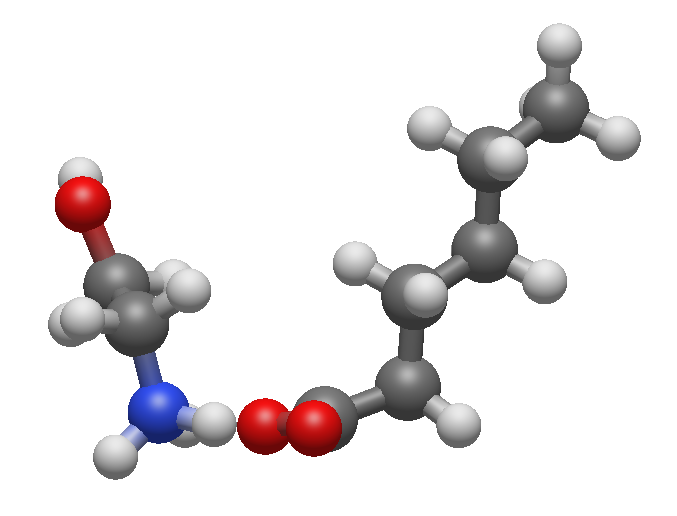
\includegraphics[width=0.42\textwidth]{imagens/2HEAHx_avogadro.png} &
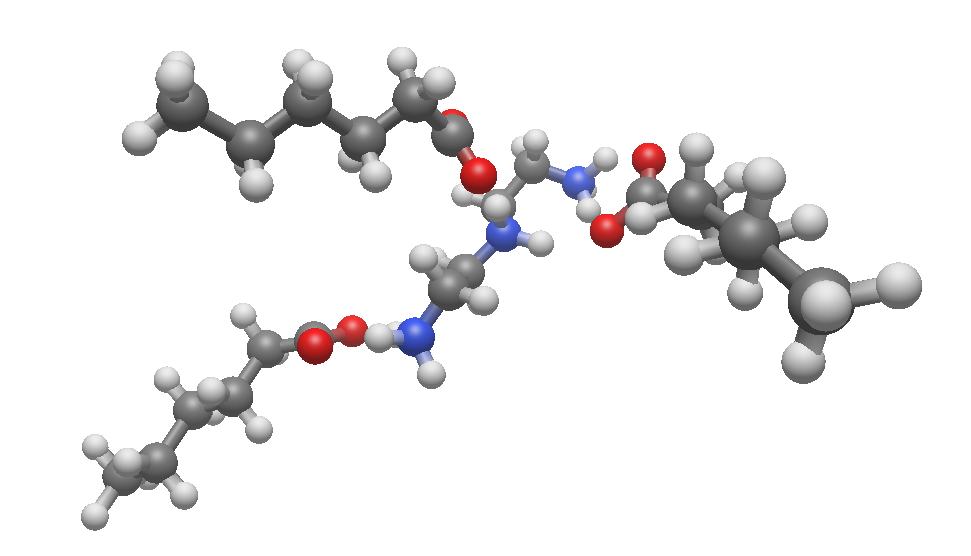
\includegraphics[width=0.42\textwidth]{imagens/DETAHx_avogadro.png} \\
(a) [2-HEA][Hx] & (b) [DETA][Hx] \\
\end{tabular}
\end{figure}

\begin{table}[H]
\caption{Propriedades físicas e estruturais das espécies envolvidas nos sistemas estudados.}
\label{tab:propriedades_especies}
\centering
\begin{tabularx}{\textwidth}{Xccc}
\toprule
\textbf{Composto} & \textbf{Abreviação} & \textbf{Fórmula molecular} & \textbf{Massa molar (g/mol)} \\
\midrule
Trioleína & --- & C\textsubscript{57}H\textsubscript{104}O\textsubscript{6} & 885,4 \\
Trilinoleína & --- & C\textsubscript{57}H\textsubscript{98}O\textsubscript{6} & 879,4 \\
Trilinolenina & --- & C\textsubscript{57}H\textsubscript{92}O\textsubscript{6} & 873,3 \\
Ácido oleico & --- & C\textsubscript{18}H\textsubscript{34}O\textsubscript{2} & 282,5 \\
Ácido linoleico & --- & C\textsubscript{18}H\textsubscript{32}O\textsubscript{2} & 280,4 \\
Etanol & --- & C\textsubscript{2}H\textsubscript{6}O & 46,1 \\
Metanol & --- & CH\textsubscript{4}O & 32,0 \\
Hexanoato de 2-hidroxietilamônio & [2-HEA][Hx] & C\textsubscript{8}H\textsubscript{19}NO\textsubscript{3} & 177,2 \\
Hexanoato de dietilenotriamônio & [DETA][Hx] & C\textsubscript{22}H\textsubscript{49}N\textsubscript{3}O\textsubscript{6} & 451,6 \\
\bottomrule
\end{tabularx}
\end{table}

\section{Cálculos DFT/COSMO e origem dos \texorpdfstring{$\sigma$}{sigma}-profiles}
\label{sec:dft_cosmo}

A qualidade das predições do modelo COSMO-SAC depende da consistência entre o nível de teoria empregado na geração dos $\sigma$-profiles e a parametrização adotada no cálculo dos coeficientes de atividade (Seção \ref{subsec:cosmo_parametros}). Neste trabalho, todos os $\sigma$-profiles utilizados são compatíveis com a parametrização GAMESS implementada no JCOSMO, conforme documentado por \citeonline{wang2009}.

Para o etanol, o metanol, a trioleína, a trilinoleína e a trilinolenina, os $\sigma$-profiles foram obtidos diretamente da base de dados interna do JCOSMO, que contém perfis pré-calculados para um conjunto extenso de compostos orgânicos convencionais \cite{mullins2006}. Os cálculos originais dessa base foram realizados no pacote GAMESS \cite{gamess2020} com o nível de teoria e os parâmetros de cavidade descritos por \citeonline{wang2009}, o que garante a consistência com a parametrização do modelo.

Para os pares iônicos neutros [2-HEA][Hx] e [DETA][Hx], que não constam na base interna do JCOSMO, os $\sigma$-profiles foram gerados por cálculos DFT/COSMO realizados no pacote GAMESS \cite{gamess2020}, seguindo o procedimento descrito por \citeonline{wang2009} para garantir a compatibilidade com a parametrização do modelo. Cada par foi calculado como uma única molécula neutra (carga total 0), conforme a estratégia de par iônico neutro adotada neste trabalho (Seção \ref{sec:cosmo_li}), e não como cátion e ânion isolados. A otimização de geometria e a determinação das cargas de blindagem no contínuo dielétrico foram realizadas de forma simultânea e autoconsistente, conforme descrito na Seção \ref{sec:cosmo_solvatacao}. Os arquivos de saída no formato \texttt{.gout} gerados pelo GAMESS foram importados diretamente no JCOSMO como compostos personalizados.

A Tabela \ref{tab:cosmo_detalhes} resume a origem dos
$\sigma$-profiles de cada espécie.

\begin{table}[H]
    \centering
    \caption{Origem dos $\sigma$-profiles utilizados nos cálculos COSMO-SAC (parametrização GAMESS no JCOSMO).}
    \label{tab:cosmo_detalhes}
    \begin{tabular}{lccc}
        \toprule
        \textbf{Espécie} & \textbf{Carga} &
        \textbf{N$^{\circ}$ de átomos} & \textbf{Origem} \\
        \midrule
        Etanol             &  0 &   9 & Base interna do JCOSMO \\
        Metanol            &  0 &   6 & Base interna do JCOSMO \\
        Trioleína          &  0 & 167 & Base interna do JCOSMO \\
        Trilinoleína       &  0 & 161 & Base interna do JCOSMO \\
        Trilinolenina      &  0 & 155 & Base interna do JCOSMO \\
        Ácido oleico       &  0 &  54 & Base interna do JCOSMO \\
        Ácido linoleico    &  0 &  52 & Base interna do JCOSMO \\
        {[2-HEA][Hx]} (par neutro) &  0 &  31 & Calculado no GAMESS \\
        {[DETA][Hx]} (par neutro)  &  0 &  80 & Calculado no GAMESS \\
        \bottomrule
    \end{tabular}
\end{table}

A geração da tabela de segmentos de superfície (área e carga de blindagem por segmento), necessária para a construção do $\sigma$-profile de cada par iônico neutro, exigiu uma modificação prévia no código-fonte do GAMESS. Na compilação padrão do pacote, essa tabela não é impressa no arquivo de saída, independentemente das palavras-chave de entrada utilizadas. A solução, documentada no repositório do Laboratório Virtual de Predição de Propriedades (LVPP)\footnote{Disponível em: \url{https://github.com/lvpp/sigma}.}, mesmo banco de dados de $\sigma$-profiles do qual o JCOSMO se utiliza, consiste em um patch aplicado ao arquivo-fonte \texttt{cosprt.src} antes da compilação, responsável pela rotina de impressão dos dados COSMO. Após a aplicação desse patch e a recompilação do GAMESS, a tabela de segmentos passou a ser impressa automaticamente, tornando desnecessária (e, em combinação com a base \texttt{d2tzvp} empregada, incompatível) a palavra-chave de entrada \texttt{COSWRT=.TRUE.}, que foi removida do arquivo de configuração dos cálculos.

A escolha de utilizar a base interna do JCOSMO para o etanol, o metanol, a trioleína, a trilinoleína e a trilinolenina, em vez de realizar novos cálculos, assegura que os $\sigma$-profiles dessas espécies são exatamente aqueles para os quais os parâmetros universais do modelo foram calibrados, evitando inconsistências que poderiam comprometer a qualidade das predições. Para os pares neutros dos LIPs, por não estarem disponíveis em nenhuma base pré-existente, o cálculo no GAMESS com o mesmo nível de teoria da base é a única forma de garantir essa consistência.

\section{Geração dos \texorpdfstring{$\sigma$}{sigma}-profiles e cálculo do ELL no JCOSMO}
\label{sec:jcosmo}

O cálculo dos coeficientes de atividade pelo modelo COSMO-SAC e a determinação do equilíbrio líquido-líquido foram realizados no \textit{software} JCOSMO, desenvolvido pelo Laboratório Virtual de Predição de Propriedades (LVPP) da Universidade Federal do Rio Grande do Sul (UFRGS) \cite{gerber2010}. O JCOSMO é uma implementação de código aberto, em linguagem Java, dos modelos COSMO-SAC e suas variantes, que permite a importação de $\sigma$-profiles a partir de diferentes pacotes de química quântica (GAMESS, TURBOMOLE, DMol3, MOPAC), o cálculo de coeficientes de atividade, testes de estabilidade de fases e a construção de diagramas de equilíbrio de fases para sistemas multicomponentes.

A execução da interface gráfica do JCOSMO em versões recentes do Java (Java 21) exigiu um ajuste na linha de comando de inicialização. A biblioteca de serialização empregada internamente pelo JCOSMO (XStream) tenta acessar, por reflexão, classes internas de módulos do Java que passaram a ser encapsulados por padrão a partir do sistema de módulos introduzido nas versões mais recentes da plataforma, o que resulta em uma exceção (\texttt{InaccessibleObjectException}) e impede a abertura do programa. A solução consiste em iniciar o JCOSMO explicitando um conjunto de flags \texttt{--add-opens}, que reabrem manualmente os pacotes necessários (dos módulos \texttt{java.base} e \texttt{java.desktop}) para acesso por reflexão, por exemplo:

\begin{verbatim}
java --add-opens java.base/java.lang=ALL-UNNAMED \
     --add-opens java.base/java.util=ALL-UNNAMED \
     --add-opens java.desktop/java.awt=ALL-UNNAMED \
     --add-opens java.desktop/javax.swing=ALL-UNNAMED \
     -jar jcosmo.jar
\end{verbatim}
% -----------------------------------------------------------------
% Escolha da variante do modelo
% -----------------------------------------------------------------

O JCOSMO disponibiliza diferentes parametrizações do COSMO-SAC, associadas aos diferentes níveis de teoria utilizados na geração dos $\sigma$-profiles. Neste trabalho, adotou-se a parametrização correspondente ao modelo GAMESS, que utiliza $\sigma$-profiles gerados com o pacote GAMESS conforme descrito por \citeonline{wang2009}. A escolha dessa parametrização foi motivada por testes preliminares nos quais uma rota alternativa (cálculos em NWChem, cujos $\sigma$-profiles seriam posteriormente compatibilizados com a parametrização TURBOMOLE do JCOSMO) produziu resultados fisicamente inconsistentes para o sistema em estudo: as cavidades moleculares geradas apresentaram dimensões significativamente superiores às esperadas (da ordem de quatro vezes a área esperada para a trioleína), resultando em $\sigma$-profiles excessivamente suavizados e em predições de afinidade trioleína-etanol incompatíveis com o comportamento experimental conhecido (miscibilidade parcial). Essa rota foi descartada, e os cálculos dos pares iônicos neutros deste trabalho foram refeitos diretamente no GAMESS (Seção~\ref{sec:dft_cosmo}), que produziu $\sigma$-profiles com distribuições de carga fisicamente coerentes; para as demais sete espécies, disponíveis na base de dados interna do JCOSMO, essa questão não se colocou, já que seus $\sigma$-profiles já haviam sido calculados e validados previamente pelo desenvolvedor da ferramenta.


% -----------------------------------------------------------------
% Incorporação dos σ-profiles dos LIPs
% -----------------------------------------------------------------

A base de dados interna do JCOSMO para o modelo GAMESS contém $\sigma$-profiles pré-calculados para um conjunto extenso de compostos orgânicos convencionais \cite{mullins2006}, incluindo os sete compostos moleculares deste trabalho (etanol, metanol, trioleína, trilinoleína, trilinolenina, ácido oleico e ácido linoleico). Os pares iônicos neutros [2-HEA][Hx] e [DETA][Hx], contudo, não constam dessa base, o que exigiu a incorporação dos $\sigma$-profiles gerados pelos cálculos DFT/COSMO realizados diretamente no GAMESS (Seção~\ref{sec:dft_cosmo}). Os arquivos \texttt{.gout} resultantes desses cálculos foram importados no JCOSMO como compostos personalizados, seguindo o mesmo procedimento de importação empregado para qualquer molécula neutra.

Uma vez que os $\sigma$-profiles de todas as nove espécies estavam disponíveis no JCOSMO, a configuração dos sistemas ternários foi feita diretamente na aba \textit{Mixture} do programa, inserindo cada líquido iônico prótico como um composto puro regular (o par neutro [2-HEA][Hx] ou [DETA][Hx]), na mesma condição dos demais componentes do sistema (triglicerídeo e álcool). Essa abordagem dispensa qualquer funcionalidade de combinação de íons separados, já que o par neutro já constitui, por si só, a unidade química completa cujo $\sigma$-profile foi previamente calculado e importado. O próprio JCOSMO normaliza internamente as frações molares informadas para cada componente da mistura, de modo que a composição do sistema ternário é definida diretamente pelas frações molares dos três compostos puros (triglicerídeo, álcool e par iônico neutro), sem etapas intermediárias de conversão.

% -----------------------------------------------------------------
% Cálculo do ELL
% -----------------------------------------------------------------

O JCOSMO é empregado exclusivamente para o cálculo dos coeficientes de atividade $\gamma_i$ de cada componente, a partir dos $\sigma$-profiles importados e da composição da mistura definida na aba \textit{Mixture}. O programa não realiza nativamente a construção de diagramas de equilíbrio de fases, de modo que o teste de estabilidade, o cálculo \textit{flash} líquido-líquido e a construção do diagrama ternário são realizados externamente, nos mesmos módulos Python desenvolvidos para o UNIFAC-LL (Seção \ref{sec:unifac_implementacao}), adaptados para consumir os coeficientes de atividade calculados pelo JCOSMO em vez dos calculados internamente pela rotina UNIFAC-LL. A comunicação entre o JCOSMO (em Java) e os módulos de estabilidade e flash (em Python) é feita por meio da biblioteca py4j, que expõe os métodos de cálculo de $\gamma_i$ do JCOSMO como uma ponte acessível diretamente do código Python.

O procedimento de cálculo do equilíbrio líquido-líquido, executado nesses módulos Python, compreende três etapas. A primeira é o teste de estabilidade de fases (critério TPD, Seção \ref{sec:ell_fundamentos}), que verifica, para uma dada composição global, se a mistura é estável como fase única ou se existe uma configuração de duas fases com energia de Gibbs total inferior. A segunda etapa é o cálculo \textit{flash} líquido-líquido, que determina as composições e as quantidades relativas das duas fases em equilíbrio a partir da composição global, resolvendo iterativamente a condição de isoatividade (Equação \ref{eq:isoatividade}) para todos os componentes do sistema. A terceira etapa é a construção do diagrama ternário, na qual o procedimento de teste de estabilidade e cálculo flash é repetido sistematicamente para uma malha de composições globais que cobre o interior do triângulo ternário, permitindo traçar a curva binodal e as linhas de amarração.

Todos os cálculos de ELL foram realizados a 298,15 K e pressão atmosférica, condições consistentes com os dados experimentais de validação (Seção \ref{sec:dados_validacao}) e com as condições empregadas nos estudos experimentais de referência \cite{trindade2019,gomez2019}.

\section{Implementação do UNIFAC-LL}
\label{sec:unifac_implementacao}

Toda a ferramenta computacional empregada neste trabalho para o cálculo do equilíbrio líquido-líquido e para a construção dos diagramas ternários foi desenvolvida pela autora, em linguagem Python, sem recurso a bibliotecas termodinâmicas prontas para essas finalidades. O conjunto é organizado em módulos com funções específicas: o cálculo dos coeficientes de atividade pelo UNIFAC-LL (contribuições combinatorial e residual), o teste de estabilidade de fases, o cálculo \textit{flash} líquido-líquido, a localização do ponto crítico, a renderização dos diagramas ternários, a interface gráfica de seleção de sistemas e o executor de fila que processa múltiplos sistemas em sequência. Empregaram-se apenas bibliotecas de uso geral (NumPy para álgebra numérica, Matplotlib para renderização e py4j para a comunicação com o JCOSMO), de modo que a formulação termodinâmica, os algoritmos de equilíbrio e a construção geométrica dos diagramas são de implementação própria.
 
Essa autoria tem uma implicação metodológica direta: como nenhuma etapa do cálculo é herdada de implementação de terceiros já validada, tornou-se necessário verificar a corretude do próprio motor de cálculo antes de aplicá-lo aos sistemas de interesse, o que é feito em duas etapas independentes descritas na Seção~\ref{sec:validacao_computacional}. A única exceção é o cálculo dos coeficientes de atividade pelo COSMO-SAC, delegado ao JCOSMO (Seção~\ref{sec:jcosmo}); todas as demais etapas, inclusive as que consomem esses coeficientes, pertencem ao código desenvolvido neste trabalho.
 
Os parâmetros de volume ($R_k$) e de área superficial ($Q_k$) dos grupos funcionais, bem como os parâmetros de interação binários ($a_{mn}$), foram extraídos da parametrização de \citeonline{magnussen1981} para equilíbrio líquido-líquido.

A implementação computacional do modelo UNIFAC-LL foi realizada em linguagem Python, organizada em módulos com funções específicas: cálculo dos coeficientes de atividade (combinatorial e residual), teste de estabilidade de fases, cálculo flash líquido-líquido e construção dos diagramas ternários. Os parâmetros de volume ($R_k$) e área superficial ($Q_k$) dos grupos funcionais, bem como os parâmetros de interação binários ($a_{mn}$), foram extraídos da parametrização de \citeonline{magnussen1981} para equilíbrio líquido-líquido, com valores complementares obtidos de \citeonline{bessa2016}.

O teste de estabilidade de fases e o cálculo flash reutilizam os mesmos módulos empregados para o COSMO-SAC (Seção \ref{sec:jcosmo}), com o coeficiente de atividade fornecido pela rotina UNIFAC-LL em vez do JCOSMO. O teste de estabilidade aplica o critério do plano tangente (TPD, Equação \ref{eq:tpd}, Seção \ref{sec:ell_fundamentos}), avaliando a função $TPD(\mathbf{x})$ para um conjunto de composições de teste distribuídas sobre o simplex ternário; a composição global é considerada instável sempre que algum ponto de teste produz $TPD(\mathbf{x}) < 0$, sinalizando a necessidade de separação em duas fases. Uma vez identificada a instabilidade, o cálculo flash resolve iterativamente a condição de isoatividade (Equação \ref{eq:isoatividade}) por meio de substituições sucessivas, ajustando as composições de tentativa das duas fases até que a razão $K_i = \gamma_i^{I}/\gamma_i^{II}$ de cada componente convirja dentro de uma tolerância pré-estabelecida. A construção do diagrama ternário completo repete esse procedimento para uma malha de composições globais que cobre o interior do triângulo de composições, com a curva binodal traçada a partir do conjunto de composições nas quais a transição de estável para instável ocorre.

A decomposição em grupos funcionais foi realizada para cada componente dos sistemas estudados. O etanol foi decomposto em 1 \ce{CH3} + 1 \ce{CH2} + 1 OH. A trioleína, por sua elevada massa molar e complexidade estrutural, requer uma decomposição mais extensa que inclui grupos \ce{CH3}, \ce{CH2}, CH, \ce{CH=CH} e \ce{CH2COO} (grupo éster, principal 11, denominado CCOO). Para os líquidos iônicos próticos, tratados como par iônico neutro (Seção~\ref{sec:cosmo_li}), a decomposição envolve a atribuição conjunta de grupos do cátion e do ânion, incluindo \ce{CH2}, OH, \ce{CNH2} e \ce{CNH} para as porções aminadas, e COO (grupo principal 41) para o carboxilato do ânion hexanoato, conforme detalhado na Tabela~\ref{tab:decomposicao_unifac}. O grupo COO empregado para o ânion é um grupo isolado (apenas o carbono carboxílico e os dois oxigênios), distinto do grupo éster CCOO presente nos triglicerídeos: o ânion hexanoato (\ce{CH3-(CH2)4-COO-}) é decomposto simplesmente como 1 \ce{CH3} + 4 \ce{CH2} + 1 COO, sem necessidade de ajuste para dupla contagem, já que nenhum desses grupos incorpora átomos de outro.

A estequiometria do par neutro [DETA][Hx] segue a proporção 1:3 entre cátion e ânion, refletindo a natureza triprotonada do cátion dietilenotriamônio: os três sítios de amônio protonado (dois terminais e um secundário, Seção \ref{sec:estruturas}) requerem três ânions hexanoato para neutralização completa da carga, na mesma estequiometria de síntese reportada por \citeonline{trindade2019} (1 mol de dietilenotriamina para 3 mol de ácido hexanoico). Essa proporção 1:3 é refletida diretamente na contagem de grupos funcionais do par neutro: os três ânions hexanoato contribuem, juntos, com o triplo dos grupos do ânion isolado (3 \ce{CH3} + 12 \ce{CH2} + 3 COO), somados aos grupos do cátion triprotonado.

\begin{table}[H]
\caption{Decomposição das espécies em grupos funcionais UNIFAC.}
\label{tab:decomposicao_unifac}
\centering
\begin{tabularx}{\textwidth}{lX}
\toprule
\textbf{Componente} & \textbf{Decomposição em subgrupos} \\
\midrule
Etanol & 1 CH\textsubscript{3} + 1 CH\textsubscript{2} + 1 OH \\
Metanol & 1 CH\textsubscript{3} + 1 OH \\
Trioleína & 3 CH\textsubscript{3} + 41 CH\textsubscript{2} + 1 CH + 3 CH=CH + 3 CH\textsubscript{2}COO \\
Trilinoleína & 3 CH\textsubscript{3} + 35 CH\textsubscript{2} + 1 CH + 6 CH=CH + 3 CH\textsubscript{2}COO \\
Trilinolenina & 3 CH\textsubscript{3} + 29 CH\textsubscript{2} + 1 CH + 9 CH=CH + 3 CH\textsubscript{2}COO \\
Ácido oleico & 1 CH\textsubscript{3} + 14 CH\textsubscript{2} + 1 CH=CH + 1 COOH \\
Ácido linoleico & 1 CH\textsubscript{3} + 12 CH\textsubscript{2} + 2 CH=CH + 1 COOH \\
{[2-HEA][Hx]} (par neutro) & 1 OH + 6 CH\textsubscript{2} + 1 CNH\textsubscript{2} + 1 CH\textsubscript{3} + 1 COO \\
{[DETA][Hx]} (par neutro) & 12 CH\textsubscript{2} + 2 CNH\textsubscript{2} + 2 CNH + 3 CH\textsubscript{3} + 3 COO \\
\bottomrule
\end{tabularx}
\end{table}

A validação da implementação foi realizada com o sistema ternário \{n-hexano + etanol + água\} a 298,15 K, para o qual dados experimentais de ELL estão disponíveis na literatura e todos os parâmetros de interação binários entre os grupos envolvidos constam na matriz de \citeonline{magnussen1981}. O diagrama ternário simulado foi comparado com os dados experimentais de \citeonline{sorensen1980}, obtendo-se um desvio quadrático médio (RMSD) das frações molares nas linhas de amarração de 0,0872, o que confirma a corretude da implementação para sistemas em que a parametrização é completa.

% -----------------------------------------------------------------
% Parâmetros ausentes: preenchimento por modelo de ML
% -----------------------------------------------------------------

A matriz de \citeonline{magnussen1981} não contém parâmetros de interação para dez pares de grupos necessários aos sistemas estudados neste trabalho: quatro pares específicos dos grupos amino e carboxilato dos líquidos iônicos próticos (CCOO(11)/CNH$_2$(14), CNH$_2$(14)/CCOO(11), CNH$_2$(14)/COO(41) e COO(41)/CNH$_2$(14)) e seis pares envolvendo o grupo carboxila dos ácidos graxos livres (COOH(20)/CH2(1), COOH(20)/C=C(2), COOH(20)/OH(5), COOH(20)/CNH2(14), COOH(20)/CNH(15) e COOH(20)/COO(41)). Todos os dez foram preenchidos com os valores preditos pelo modelo de aprendizado de máquina UNIFAC 2.0 de \citeonline{hayer2025}, que preserva o framework original de Fredenslund e os mesmos parâmetros $R_k$/$Q_k$ de \citeonline{magnussen1981} para os grupos relevantes deste trabalho, o que garante compatibilidade direta com o restante da matriz de interação empregada neste trabalho. A Tabela~\ref{tab:parametros_ml_pil} apresenta os dez valores adotados.

\begin{longtable}{lc}
\caption{Parâmetros de interação preenchidos pelo modelo UNIFAC 2.0 (Hayer, Wendel, Mandt, Hasse \& Jirásek, 2025).}
\label{tab:parametros_ml_pil} \\
\toprule
\textbf{Par ($a_{mn}$, K)} & \textbf{Valor} \\
\midrule
\endfirsthead

\multicolumn{2}{c}{\tablename\ \thetable\ -- continuação} \\
\toprule
\textbf{Par ($a_{mn}$, K)} & \textbf{Valor} \\
\midrule
\endhead

\bottomrule
\endfoot

\multicolumn{2}{l}{\textit{Grupos do líquido iônico prótico}} \\
CCOO(11)/CNH$_2$(14) & 53,04 \\
CNH$_2$(14)/CCOO(11) & 22,94 \\
CNH$_2$(14)/COO(41)  & $-$69,50 \\
COO(41)/CNH$_2$(14)  & 20,76 \\
\addlinespace
\multicolumn{2}{l}{\textit{Grupos dos ácidos graxos livres}} \\
COOH(20)/CH2(1)   & 168,73 \\
CH2(1)/COOH(20)   & 470,64 \\
COOH(20)/C=C(2)   & 145,55 \\
C=C(2)/COOH(20)   & 449,47 \\
COOH(20)/OH(5)    & $-$128,55 \\
OH(5)/COOH(20)    & $-$13,35 \\
COOH(20)/CNH$_2$(14) & $-$96,50 \\
CNH$_2$(14)/COOH(20) & $-$270,83 \\
COOH(20)/CNH(15)  & $-$159,72 \\
CNH(15)/COOH(20)  & $-$376,90 \\
COOH(20)/COO(41)  & $-$24,18 \\
COO(41)/COOH(20)  & 226,12 \\

\end{longtable}

A adoção desses valores, em vez de uma calibração direta contra sistemas análogos, decorre da natureza mesma da lacuna: os sistemas experimentais disponíveis para calibração direta desses grupos são escassos e estruturalmente distantes dos sistemas-alvo deste trabalho (Seção~\ref{subsec:parametros_perfis}), de modo que uma calibração dedicada correria o risco de ajustar os parâmetros às particularidades de um conjunto pequeno e pouco representativo de dados, sem garantia de generalização para o sistema \{triglicerídeo + álcool + PIL\} de interesse. Os valores de \citeonline{hayer2025}, por sua vez, resultam de um modelo treinado sobre uma base de dados experimental ampla (\textit{Dortmund Data Bank}), o que confere maior robustez estatística ao preenchimento desses pares específicos, ainda que sem garantia de que qualquer um desses dezesseis pares tenha, especificamente, dado experimental direto por trás do valor predito.

Os valores adotados para esses dez parâmetros (Tabela~\ref{tab:parametros_ml_pil}) situam-se, em sua maioria, na faixa de dezenas a poucas centenas de Kelvin, ordem de grandeza típica dos demais parâmetros de interação da matriz de \citeonline{magnussen1981} usados neste trabalho, o que é coerente com sua origem em um modelo treinado sobre uma base de dados experimental ampla (mais de 224.000 pontos, segundo \citeonline{hayer2025}). Isso contrasta com a alternativa de uma calibração direta e dedicada a partir de um conjunto pequeno de sistemas análogos, abordagem que tende a produzir parâmetros de magnitude mais extrema quando o conjunto de calibração é limitado a poucos sistemas estruturalmente distantes do sistema-alvo, sobreajustando-se às particularidades desses poucos dados em vez de capturar o comportamento geral do par de grupos. A escolha pelos valores de \citeonline{hayer2025} não elimina, contudo, a limitação de fundo discutida na Seção~\ref{subsec:parametros_perfis}: mesmo com parâmetros de magnitude fisicamente razoável, a aplicação desses dezesseis pares aos sistemas de interesse deste trabalho (triglicerídeos C57 combinados a cátions amônio protonados, e ácidos graxos livres) permanece uma extrapolação do modelo de ML para fora do domínio químico em que foi majoritariamente treinado e validado, e essa extrapolação é uma limitação estrutural do método de contribuição de grupos aplicado a líquidos iônicos.

Conforme discutido na Seção~\ref{sec:unifacll}, a aplicação do UNIFAC-LL aos sistemas contendo os LIPs [2-HEA][Hx] e [DETA][Hx] depende, para os quatro pares de grupos específicos do PIL, de parâmetros preditos por um modelo de aprendizado de máquina treinado fora do domínio químico de interesse, e não de uma calibração direta contra dados experimentais desse tipo de sistema. Os resultados dessa aplicação, incluindo a análise das consequências dessa extrapolação sobre as predições do modelo, são apresentados no Capítulo~\ref{cap:resultados}.

\section{Métricas de avaliação dos resultados}
\label{sec:metricas}
 
Os diagramas ternários gerados pelo procedimento descrito nas seções anteriores são analisados no Capítulo~\ref{cap:resultados} por meio de um conjunto definido de grandezas, cuja obtenção se descreve a seguir.
 
A varredura do simplex de composições é conduzida sobre uma malha regular de $n_{\text{grid}} = 20$ divisões por aresta, idêntica para os dois modelos termodinâmicos e para todos os sistemas, de modo que os resultados sejam comparáveis entre si. Cada composição global da malha é submetida ao teste de estabilidade e, quando instável, ao cálculo \textit{flash}, do qual resulta uma linha de amarração. Adotam-se como critérios de aceitação da solução não trivial $0{,}01 < \psi < 0{,}99$, em que $\psi$ é a fração da fase secundária, e $|x^{\alpha} - x^{\beta}| > 0{,}02$, o que descarta convergências para a solução trivial em que as duas fases coincidem.
 
A extensão da região bifásica é quantificada pela área delimitada pela curva binodal, obtida por integração poligonal sobre as extremidades das linhas de amarração e expressa em fração da área total do simplex. O ponto crítico, no qual as duas fases se tornam indistinguíveis, é estimado por encolhimento sucessivo da largura da região instável, procedimento que se mostrou numericamente mais estável do que a alternativa baseada em Newton-Raphson aplicado à condição de forma cúbica da superfície de energia de Gibbs. A distância entre os pontos críticos estimados por cada modelo para um mesmo sistema é calculada como distância euclidiana no espaço de frações molares.
 
A avaliação do efeito do líquido iônico prótico sobre a miscibilidade apoia-se em duas grandezas adicionais. As composições das extremidades de todas as linhas de amarração de um sistema são classificadas em ramo rico em óleo e ramo rico em álcool e agrupadas em dez faixas de fração molar de líquido iônico, adotando-se como fração de referência de cada linha a média entre os valores das duas fases, uma vez que o líquido iônico se distribui de forma desigual entre elas. Em cada faixa calculam-se a largura da lacuna de imiscibilidade, definida como a diferença de fração molar de triglicerídeo entre os dois ramos, e a fração molar média de triglicerídeo no ramo alcoólico. A tendência de cada sistema é resumida pela inclinação da regressão linear da largura contra a fração de líquido iônico, cujo sinal indica se o composto aproxima ou afasta as fases coexistentes.
 
O coeficiente de distribuição de cada componente entre as fases é calculado como $K_i = x_i^{\text{fase rica em álcool}}/x_i^{\text{fase rica em óleo}}$. Registre-se que o algoritmo de \textit{flash} deixa de distinguir uma fração molar de zero absoluto abaixo de $10^{-6}$, limiar que constitui o limite de resolução do método e que se torna relevante para as espécies fortemente excluídas de uma das fases.
 
Por fim, a comparação com dados experimentais, quando disponíveis, é feita pelo desvio quadrático médio (RMSD) das frações molares nas linhas de amarração, calculado segundo
 
\begin{equation}
    \mathrm{RMSD} = \sqrt{\frac{\sum_{k}\sum_{i}\sum_{j}
    \left(x_{ijk}^{\exp} - x_{ijk}^{\mathrm{calc}}\right)^2}{6\,N}}
    \label{eq:rmsd}
\end{equation}
 
\noindent em que $x_{ijk}$ é a fração molar do componente $i$ na fase $j$ da linha de amarração $k$, e $N$ é o número de linhas de amarração do conjunto experimental.
 
% ================================================================

\chapter{Resultados e discussão}
\label{cap:resultados}

Os resultados obtidos na modelagem do equilíbrio líquido-líquido dos sistemas ternários \{triglicerídeo + álcool + líquido iônico prótico\} a 298,15~K são apresentados neste capítulo segundo os dois modelos empregados, o UNIFAC-LL e o COSMO-SAC. Como não há, na literatura, dados experimentais de equilíbrio de fases para nenhum dos doze sistemas estudados (Seção~\ref{sec:dados_validacao}), não é possível verificar as predições contra medida direta nem arbitrar entre os dois modelos quando eles divergem, de modo que o que se apresenta adiante é a descrição do que cada modelo prevê, acompanhada da procedência e das incertezas de cada dado de entrada.

A exposição parte da validação da ferramenta computacional (Seção~\ref{sec:validacao_computacional}), passa à descrição do comportamento de fases previsto por cada modelo (Seção~\ref{sec:resultados_por_sistema}), confronta esses resultados com a hipótese de cossolvência que motiva o trabalho (Seção~\ref{sec:cossolvencia}), discute os mecanismos moleculares que sustentariam o comportamento observado (Seção~\ref{sec:interpretacao_fisicoquimica}) e encerra com a síntese do que os dois modelos estabelecem em conjunto, daquilo em que divergem e do que permanece indeterminado (Seção~\ref{subsec:sintese}).

\section{Validação da ferramenta computacional}
\label{sec:validacao_computacional}

Os resultados discutidos ao longo deste capítulo dependem inteiramente da correção da ferramenta computacional empregada para gerar os diagramas de equilíbrio líquido-líquido, e essa correção foi estabelecida em duas etapas complementares. A primeira isola o motor de cálculo, isto é, os algoritmos de estabilidade de fases, flash líquido-líquido e localização do ponto crítico, testando-o independentemente do modelo termodinâmico empregado (Seção~\ref{subsec:motor_termodinamico}); a segunda caracteriza os dados de entrada específicos de cada modelo, os pares de interação do UNIFAC-LL e os perfis sigma do COSMO-SAC, incluindo o diagnóstico de qualidade que revelou o enovelamento discutido na Seção~\ref{subsec:parametros_perfis}. Tal separação entre motor e modelo é o que permite, adiante, atribuir a origem de eventuais resultados fisicamente implausíveis, distinguindo uma falha na implementação numérica de um problema na parametrização do sistema.

\subsection{Motor termodinâmico}
\label{subsec:motor_termodinamico}

Um erro na predição de um sistema ternário pode ter duas origens bastante distintas, uma falha no modelo de coeficiente de atividade (parâmetros de interação incorretos ou mal extrapolados) ou uma falha no algoritmo que consome esses coeficientes para construir o diagrama de fases, e sem isolar essas duas fontes um resultado implausível não permite saber se o problema está na termodinâmica do sistema ou na implementação. Validou-se, por esse motivo, o motor de cálculo de forma independente do modelo, empregando-se a equação de Margules simétrica de dois parâmetros ($G^E/RT = A\,x_1 x_2$, com $A = A_{12} = A_{21}$) como caso de referência para um sistema binário, por possuir solução analítica conhecida para a curva binodal. Para $A > 2$ (limiar crítico do modelo simétrico), as composições de equilíbrio $x^{I}$ e $x^{II}$ satisfazem a condição de coexistência
\[
\ln\!\left(\frac{x}{1-x}\right) + A(1-2x) = 0,
\]
resolvida analiticamente por busca de raiz unidimensional de alta precisão. Adotando-se $A = 2{,}5$, a solução exata fornece $x^{I} = (0{,}1448,\ 0{,}8552)$ e $x^{II} = (0{,}8552,\ 0{,}1448)$, e o mesmo sistema, resolvido pelo motor completo (teste de estabilidade por TPD seguido de flash por Rachford-Rice com substituições sucessivas), convergiu para os mesmos valores, com desvio quadrático médio de $2{,}50 \times 10^{-7}$ em relação à solução analítica, o que confirma a corretude da implementação independentemente do modelo termodinâmico empregado.

O teste de estabilidade de fases foi implementado segundo o critério do plano tangente (\textit{tangent plane distance}, TPD), na formulação de Baker, Pierce e Luks e posteriormente sistematizada por Michelsen, que verifica se uma composição testada minimiza a energia livre de Gibbs da mistura em relação a qualquer perturbação de composição, sendo a composição instável, e o sistema separado em duas fases líquidas, sempre que essa condição não é satisfeita. O cálculo de flash líquido-líquido, por sua vez, foi resolvido pelo método de Rachford-Rice com substituições sucessivas, adotando-se como critérios de aceitação da solução não trivial $0{,}01 < \psi < 0{,}99$ e $|x^{\alpha} - x^{\beta}| > 0{,}02$, de modo a descartar convergências para a solução trivial (as duas fases coincidindo), problema numérico recorrente nesse tipo de algoritmo quando a estimativa inicial é inadequada. Já o ponto crítico da binodal, onde as duas fases líquidas tornam-se indistinguíveis, foi localizado por encolhimento sucessivo da largura da região instável, procedimento que se mostrou numericamente mais estável do que a alternativa inicialmente testada, baseada em Newton-Raphson aplicado à condição de forma cúbica da superfície de Gibbs.

\subsection{Parâmetros e perfis de entrada}
\label{subsec:parametros_perfis}

Validado o motor de cálculo, resta caracterizar os dados que o alimentam em cada um dos dois casos, uma vez que o UNIFAC-LL e o COSMO-SAC consomem informações de naturezas distintas (parâmetros de interação entre pares de grupos funcionais, no primeiro caso, e perfis de densidade de carga superficial, no segundo) e a procedência de cada uma precisa ser descrita separadamente. Não se pretende, aqui, estabelecer qual dos dois conjuntos de entrada é preferível, questão que os resultados deste trabalho não permitem decidir na ausência de dados experimentais de referência, mas documentar de onde veio cada dado, quais verificações se realizaram sobre ele e quais incertezas permanecem associadas a cada predição apresentada adiante.

Empregou-se, no UNIFAC-LL, a matriz de parâmetros de interação de \citeonline{magnussen1981}, que fornece a maior parte das entradas requeridas pelos sistemas estudados. Dezesseis entradas, contudo, não constam dessa tabela original (oito pares de grupos, considerados nas duas direções, uma vez que $a_{mn} \neq a_{nm}$), sendo quatro delas relativas aos grupos amino e carboxilato que compõem os líquidos iônicos próticos, nas combinações CCOO/CNH$_2$ e CNH$_2$/COO, que entram no cálculo dos doze sistemas ternários centrais deste trabalho, e as doze restantes relativas ao grupo carboxila (COOH), requeridas apenas nos sistemas com ácido graxo livre discutidos na Seção~\ref{subsec:casos_sem_separacao}. Para todas elas, adotaram-se os valores preditos pelo UNIFAC 2.0 de \citeonline{hayer2025}, reunidos na Tabela~\ref{tab:parametros_ml_pil} do Capítulo~\ref{cap:metodologia}.

Optou-se por esse preenchimento, em detrimento de uma calibração dedicada, em razão da própria escassez de dados para os grupos em questão, visto que os conjuntos experimentais disponíveis para pares que envolvam grupos amino e carboxilato em contato com ésteres de cadeia longa são pequenos e estruturalmente distantes dos sistemas-alvo, condição na qual uma regressão dedicada tende a ajustar-se às particularidades do conjunto de calibração sem garantia de generalização. Considerando-se, ainda, que o UNIFAC 2.0 preserva o arcabouço original de \citeonline{fredenslund1975} e os mesmos parâmetros $R_k$ e $Q_k$ de \citeonline{magnussen1981} para os grupos relevantes a este trabalho, a compatibilidade com o restante da matriz é direta, pois não se faz necessária qualquer conversão de escala ou termo adicional de dependência de temperatura além da forma clássica $\Psi_{mn} = \exp(-a_{mn}/T)$.

O procedimento pelo qual esses valores são obtidos condiciona a leitura dos resultados que dele dependem, e merece descrição. O UNIFAC 2.0 é um modelo de aprendizado de máquina que emprega a técnica de completamento de matriz (\textit{matrix completion}), na qual a matriz incompleta de parâmetros de interação é tratada como um objeto de baixa dimensionalidade e as entradas faltantes são inferidas a partir da estrutura estatística das entradas conhecidas, com todos os parâmetros ajustados simultaneamente contra mais de 224.000 pontos experimentais do \textit{Dortmund Data Bank} \cite{hayer2025}. Como nenhuma medida experimental nova dos pares ausentes é introduzida nesse processo, o valor adotado para um par como CCOO/CNH$_2$ ancora-se em uma inferência a partir do comportamento de outros pares presentes na base, sem que exista, por trás dele, dado de equilíbrio de fases de sistema que contenha simultaneamente esses dois grupos. Tal característica não compromete, por si só, a plausibilidade dos valores (cuja ordem de grandeza, entre dezenas e poucas centenas de Kelvin, é compatível com a dos demais parâmetros da matriz), embora delimite o alcance da predição, já que os sistemas deste trabalho combinam triglicerídeos C57 a cátions amônio protonados, combinação para a qual não se identificou sistema experimental correspondente na base de treinamento.

Durante a construção dessa matriz, observou-se ainda uma sensibilidade que merece registro. O par CCOO/COO, adotado neste trabalho com o valor de 560,20~K, participa do cálculo de todos os doze sistemas, visto que conecta o grupo éster presente nos três triglicerídeos ao grupo carboxilato do ânion hexanoato, comum aos dois líquidos iônicos próticos. Ao substituir-se esse valor por $-122{,}3$~K (registrado na base \texttt{binary.csv} distribuída com o JCOSMO), eliminou-se por completo a formação de curva binodal em todos os sistemas avaliados, inclusive naqueles em que a separação de fases aparece de forma consistente nos dois modelos. Não foi possível, dentro do escopo deste trabalho, determinar qual dos dois valores é fisicamente mais adequado, nem mapear as implicações de adotar cada um deles sobre o restante da matriz, de modo que se manteve o valor original por coerência com a parametrização de \citeonline{magnussen1981}, e a questão permanece em aberto.

Submeteu-se a implementação do UNIFAC-LL, tomada em conjunto com a matriz assim construída, a uma verificação externa contra o sistema ternário \{n-hexano + etanol + água\} a 298,15~K, escolhido por dispor de dados experimentais consolidados \cite{sorensen1980} e por ter todos os parâmetros necessários já presentes na tabela de \citeonline{magnussen1981}, o que isola a verificação da implementação da questão do preenchimento discutida acima. O desvio quadrático médio (RMSD) das frações molares nas linhas de amarração foi de 0,0872, valor compatível com a magnitude de desvio usualmente associada ao UNIFAC-LL em sistemas contendo água, o que sugere que o desvio observado reflete limitações conhecidas do modelo para esse tipo de par binário.

Do lado do COSMO-SAC, o dado de entrada é de outra natureza, pois em vez de parâmetros ajustados a pares de grupos o modelo parte do perfil sigma de cada espécie (uma distribuição da densidade de carga superficial obtida a partir da geometria molecular otimizada por cálculo quântico), que dispensa ajuste prévio a dados de equilíbrio de fases. Obtiveram-se os perfis do etanol, do metanol, da trioleína, da trilinoleína e da trilinolenina diretamente do banco de dados interno do JCOSMO, gerado a partir de cálculos GAMESS previamente validados pelo desenvolvedor da ferramenta \cite{ferrarini2018}, ao passo que os dois líquidos iônicos próticos, por não constarem desse banco, tiveram seus perfis calculados como par iônico neutro, conforme descrito na Seção~\ref{sec:dft_cosmo}. Adotou-se a parametrização COSMO-SAC-HB2 de \citeonline{hsieh2010}, que subdivide a superfície de ligação de hidrogênio em grupos do tipo hidroxila e outros grupos doadores ou aceptores. Testou-se, em contrapartida, uma rota alternativa, com cálculos em NWChem e compatibilização dos perfis resultantes com a parametrização TURBOMOLE do JCOSMO, mas essa rota foi descartada após produzir, para a trioleína, cavidades moleculares com área aproximadamente quatro vezes maior que a esperada, artefato geométrico que inviabilizou seu uso e motivou a adoção exclusiva do GAMESS.

Assim como a qualidade da predição do UNIFAC-LL depende da procedência de cada parâmetro, a do COSMO-SAC depende da geometria molecular que precede o cálculo do perfil sigma, e essa dependência revelou um problema específico no caso da trilinoleína. Inspecionaram-se individualmente os arquivos de saída do GAMESS correspondentes aos três triglicerídeos, e verificou-se que a geometria da trilinoleína registrada no banco corresponde a uma conformação enovelada (dobrada sobre si mesma), em vez da conformação estendida observada nas outras duas moléculas. O raio de giração da trilinoleína, de 14,77~\AA, situa-se bem abaixo dos 21,40~\AA\ da trioleína e dos 21,01~\AA\ da trilinolenina, e a mesma discrepância aparece na dimensão molecular máxima (43,80~\AA\ contra 66,95~\AA\ e 69,79~\AA, respectivamente), enquanto a área da cavidade COSMO resultou cerca de 15\% menor que a das outras duas moléculas (970,11~\AA$^2$ contra 1143,70~\AA$^2$ e 1090,43~\AA$^2$), consequência direta do enovelamento, porque a superfície de contato com o solvente diminui quando a molécula se dobra.

Tal compactação tem consequência direta sobre o perfil sigma, pois ao dobrar-se a cadeia apolar da trilinoleína fica parcialmente encoberta pela própria estrutura molecular enquanto os grupos éster permanecem expostos, o que eleva a fração polar da superfície para 11\%, contra 8\% na trioleína. Como o COSMO-SAC infere a afinidade entre espécies a partir da correspondência entre regiões de carga complementares, uma fração polar assim inflada tende a produzir afinidade calculada da trilinoleína com o álcool e com o líquido iônico maior do que a real. Uma inconsistência interna corrobora essa leitura, já que no par isolado \{trilinoleína + etanol\} o modelo prevê $\ln \gamma < 0$, compatível com miscibilidade completa, ao passo que no sistema ternário correspondente o mesmo modelo prevê binodal ampla, e as duas predições dificilmente seriam simultaneamente verdadeiras caso a afinidade real fosse tão alta quanto sugere o resultado binário. Sendo assim, os resultados que envolvem a trilinoleína no COSMO-SAC são apresentados adiante com ressalva explícita, e a reotimização da geometria dessa molécula, partindo de conformação inicial distinta no Avogadro, é retomada como recomendação no Capítulo~\ref{conclusao}.

Cada modelo carrega, portanto, uma incerteza de origem própria e verificável, concentrada no UNIFAC-LL na procedência de dezesseis entradas da matriz de interação e na sensibilidade do par CCOO/COO, e no COSMO-SAC na qualidade geométrica dos perfis sigma, verificada como adequada para a trioleína, a trilinolenina e os dois líquidos iônicos próticos, e comprometida no caso da trilinoleína. Essas incertezas não são comensuráveis entre si, e nenhuma delas foi quantificada contra dados experimentais dos sistemas de interesse, indisponíveis na literatura, de modo que as seções seguintes apresentam o que cada modelo prevê mantendo visível a incerteza que acompanha cada predição.

\section{Comportamento de fases previsto por cada modelo}
\label{sec:resultados_por_sistema}

Validada a ferramenta computacional, apresentam-se os diagramas ternários obtidos para os sistemas \{triglicerídeo + álcool + líquido iônico prótico\} a 298,15~K segundo os dois modelos empregados. A organização adotada agrupa os resultados pelo líquido iônico prótico envolvido, em vez de agrupá-los por modelo, uma vez que é o contraste entre [2-HEA][Hx] e [DETA][Hx] que estrutura o conjunto, com o primeiro formando região bifásica nos dois modelos e o segundo separando apenas segundo o COSMO-SAC (Seções~\ref{subsec:resultados_2hea} e~\ref{subsec:resultados_deta}). Discutem-se, na sequência, o efeito da escolha do álcool (Seção~\ref{subsec:efeito_alcool}) e o do grau de insaturação da cadeia graxa (Seção~\ref{subsec:insaturacao}) sobre a posição e a extensão da binodal, reunindo-se ao final os sistemas em que não se obteve curva ou cujo resultado exige ressalva metodológica (Seção~\ref{subsec:casos_sem_separacao}). A pergunta que motiva o trabalho, isto é, se o líquido iônico prótico atua como cossolvente do par triglicerídeo-álcool, é retomada na Seção~\ref{sec:cossolvencia} a partir dessas mesmas curvas binodais.

Uma observação de leitura aplica-se a todas as tabelas que se seguem. O número de linhas de amarração (\textit{tie lines}) registrado em cada sistema corresponde às composições da grade identificadas como instáveis e para as quais o cálculo \textit{flash} convergiu a uma solução não trivial, dentro dos critérios de aceitação adotados ($0{,}01 < \psi < 0{,}99$ e $|x^{\alpha} - x^{\beta}| > 0{,}02$; Seção~\ref{subsec:motor_termodinamico}). Como esses critérios descartam preferencialmente pontos situados junto à fronteira da binodal e nas proximidades do ponto crítico, a contagem serve de indicador da extensão da região bifásica, ao passo que a quantificação dessa extensão emprega a área obtida por integração da curva binodal, expressa em fração do simplex de composições.

\subsection{Sistemas com [2-HEA][Hx]}
\label{subsec:resultados_2hea}

Os seis sistemas que combinam o líquido iônico prótico [2-HEA][Hx] aos três triglicerídeos (trioleína, trilinoleína e trilinolenina) e aos dois álcoois (etanol e metanol) apresentaram binodal do tipo 1 nos dois modelos, isto é, uma única região de imiscibilidade delimitada por curva contínua entre dois vértices do diagrama, sem formação de uma segunda ilha de separação, e em nenhum dos seis casos se observou, em qualquer dos dois modelos, indício de binodal do tipo 2 ou de curva descontínua. A Tabela~\ref{tab:tielines_2hea} reúne o número de linhas de amarração obtido em cada caso.

\begin{table}[htb]
\centering
\caption{Número de tie-lines calculadas para os sistemas com [2-HEA][Hx]}
\label{tab:tielines_2hea}
\begin{tabular}{lcc}
\hline
Sistema & UNIFAC-LL & COSMO-SAC \\
\hline
Trioleína + Etanol      & 188 & 362 \\
Trioleína + Metanol     & 257 & 368 \\
Trilinoleína + Etanol   & 207 & 345 \\
Trilinoleína + Metanol  & 267 & 365 \\
Trilinolenina + Etanol  & 303 & 327 \\
Trilinolenina + Metanol & 314 & 356 \\
\hline
\end{tabular}
\end{table}

\begin{figure}[H]
\centering
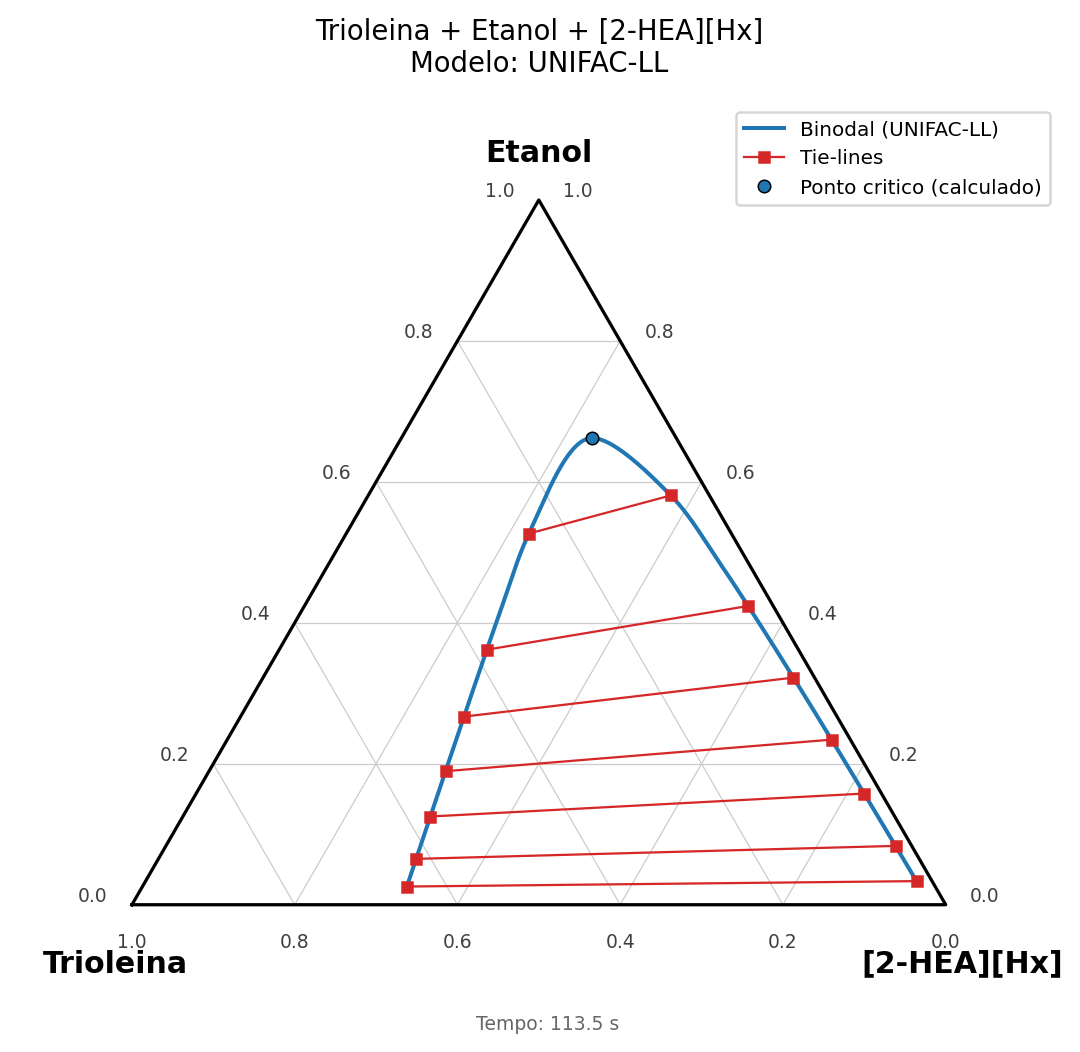
\includegraphics[width=0.4\textwidth]{imagens/ELL_Trioleina_Etanol_2_HEAHx_UNIFAC_LL.png}
\hfill
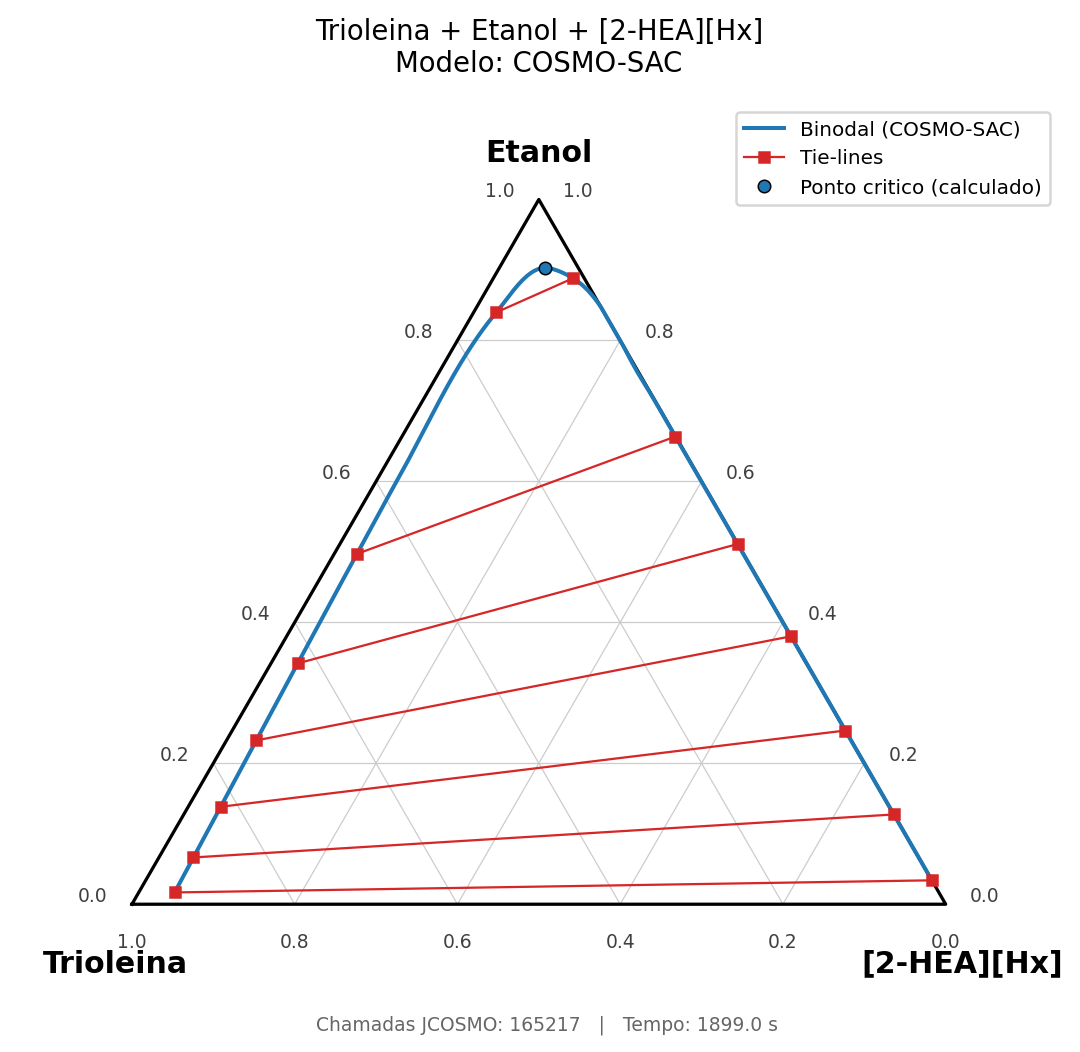
\includegraphics[width=0.4\textwidth]{imagens/ELL_Trioleina_Etanol_2_HEAHx_COSMO_SAC.png}
\caption{Trioleína + etanol + [2-HEA][Hx]: UNIFAC-LL (esquerda) e COSMO-SAC (direita)}
\label{fig:trioleina_etanol_2hea}
\end{figure}

\begin{figure}[H]
\centering
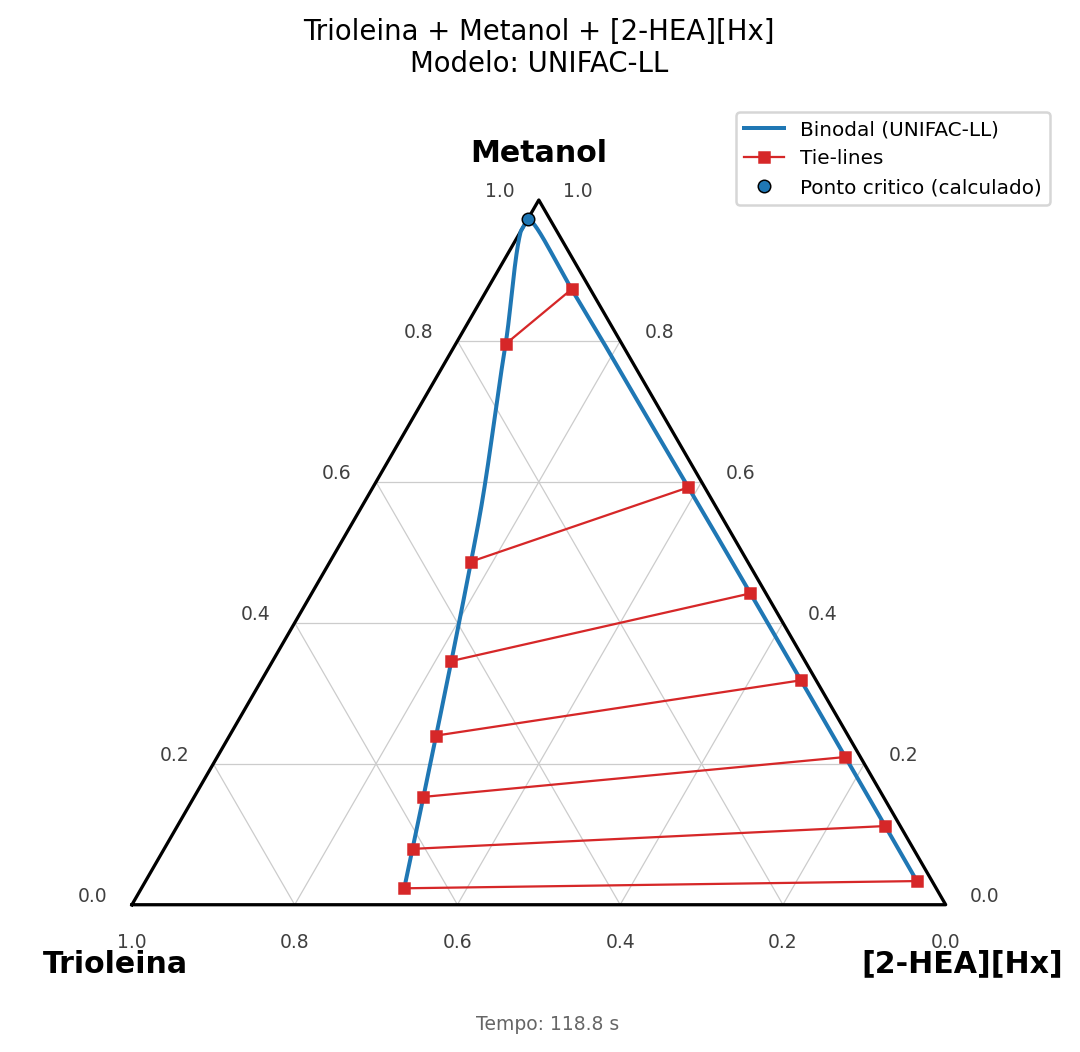
\includegraphics[width=0.4\textwidth]{imagens/ELL_Trioleina_Metanol_2_HEAHx_UNIFAC_LL.png}
\hfill
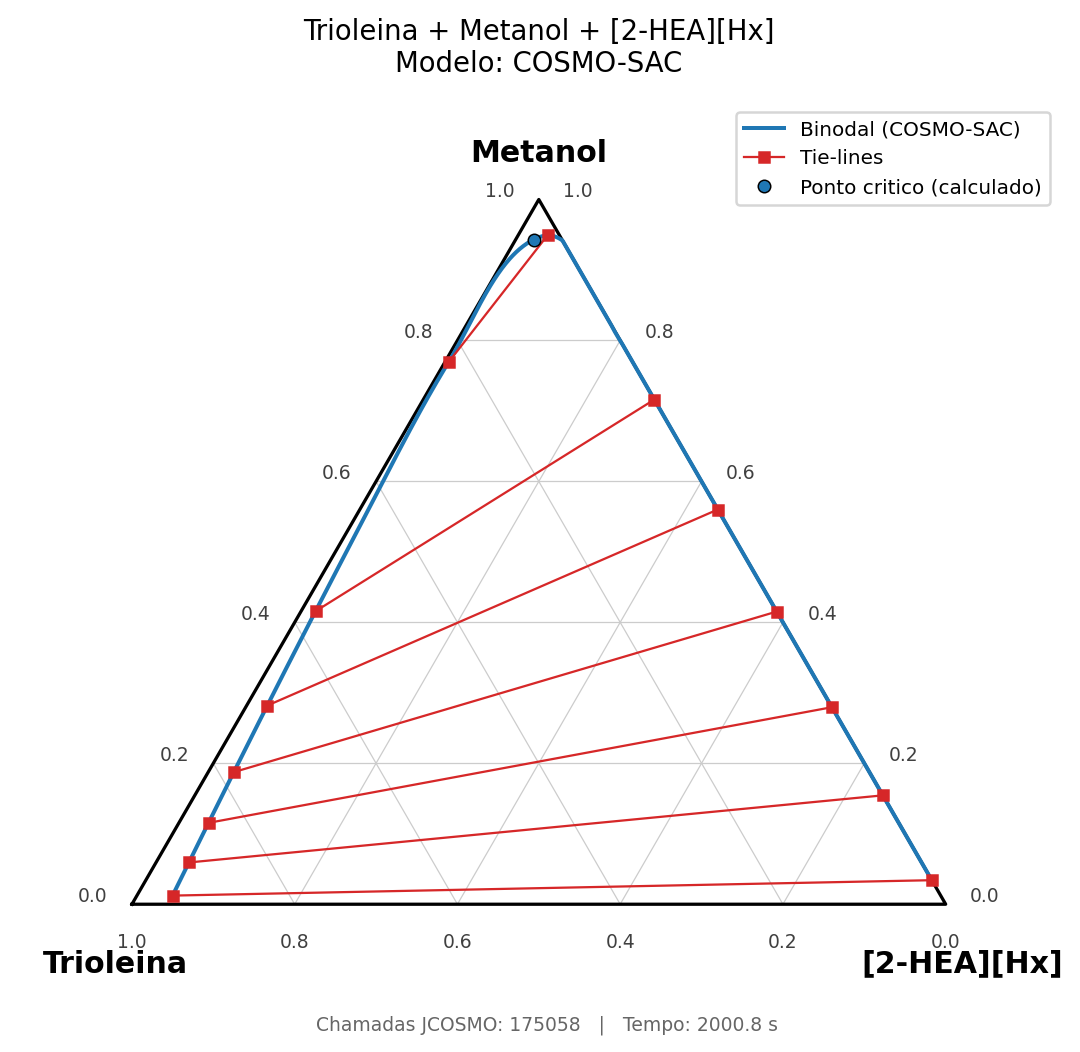
\includegraphics[width=0.4\textwidth]{imagens/ELL_Trioleina_Metanol_2_HEAHx_COSMO_SAC.png}
\caption{Trioleína + metanol + [2-HEA][Hx]: UNIFAC-LL (esquerda) e COSMO-SAC (direita)}
\label{fig:trioleina_metanol_2hea}
\end{figure}

\begin{figure}[H]
\centering
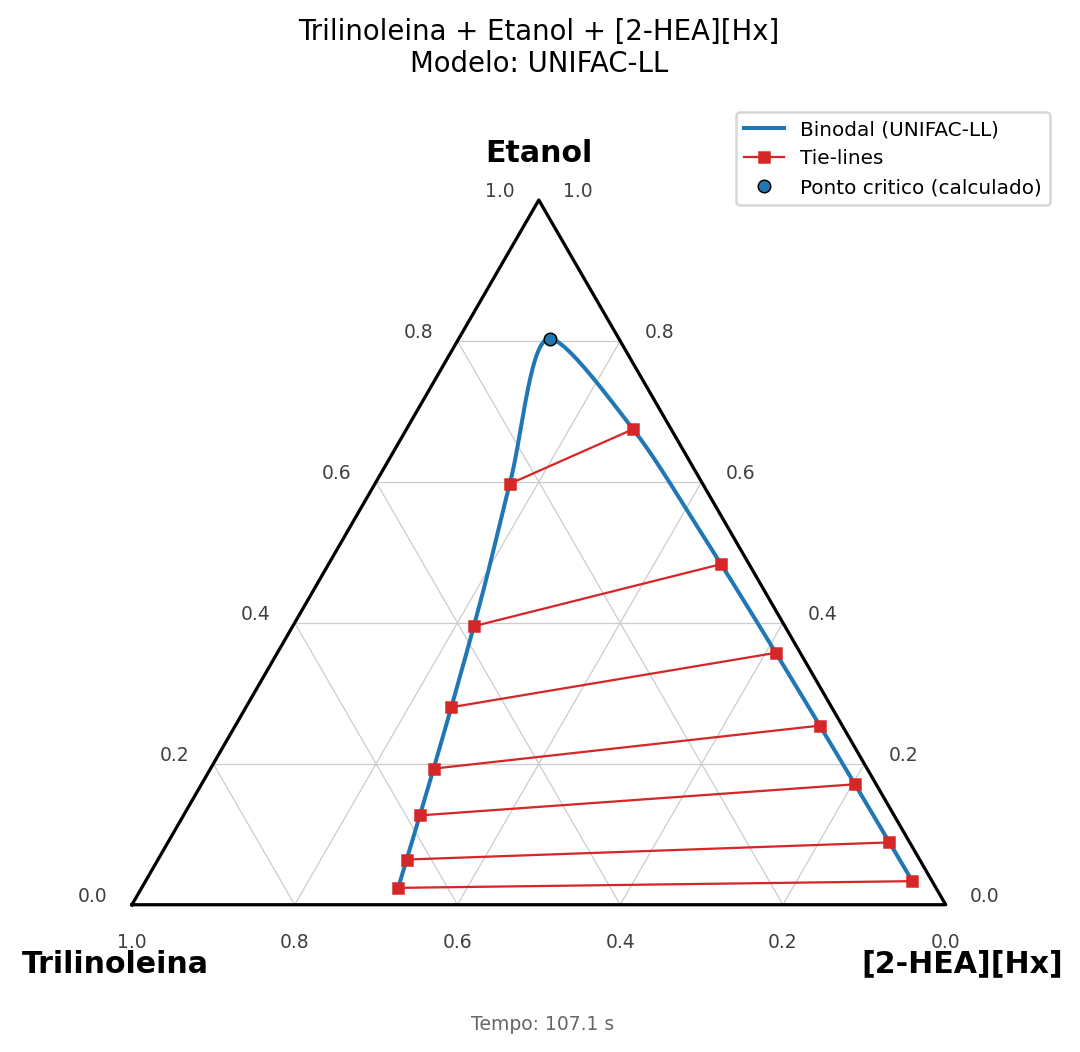
\includegraphics[width=0.4\textwidth]{imagens/ELL_Trilinoleina_Etanol_2_HEAHx_UNIFAC_LL.png}
\hfill
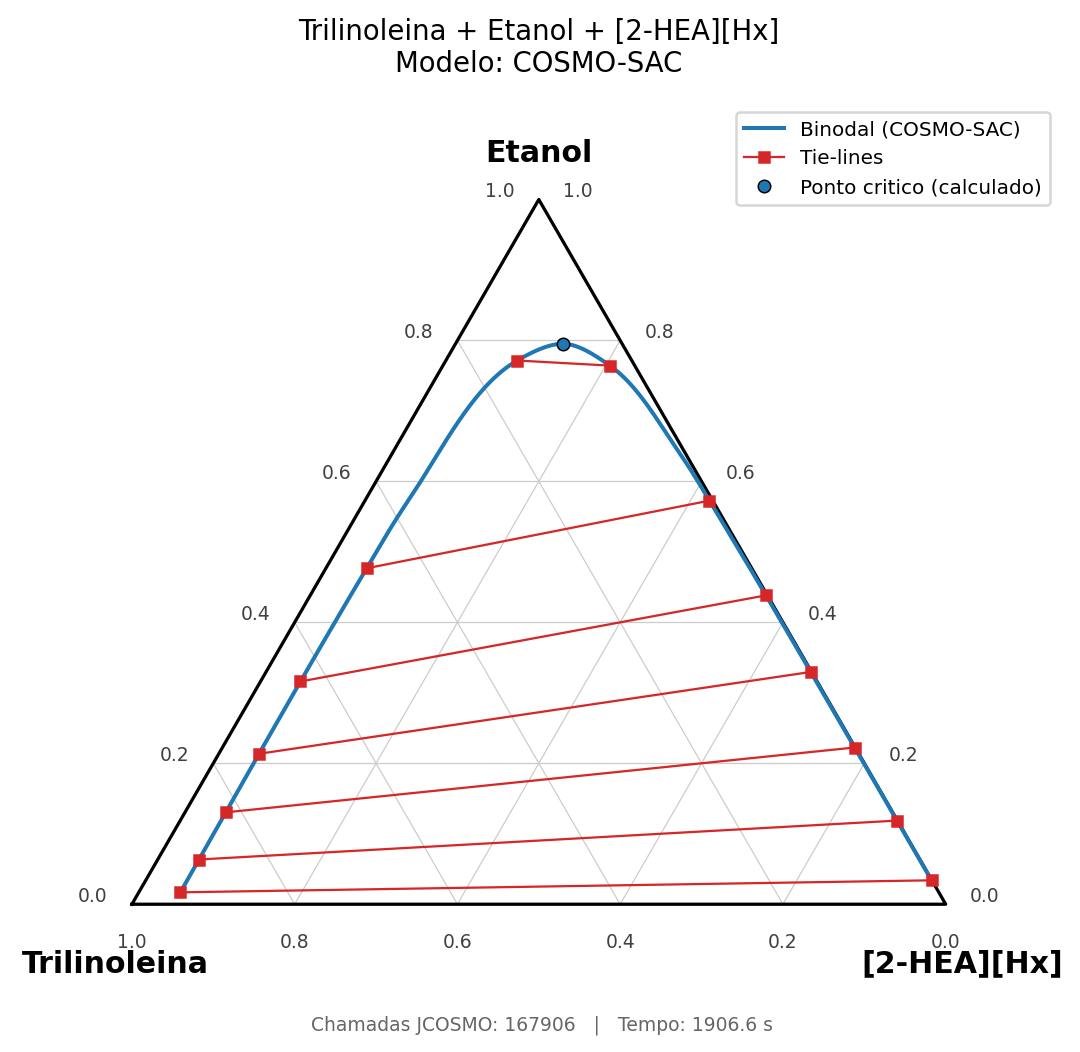
\includegraphics[width=0.4\textwidth]{imagens/ELL_Trilinoleina_Etanol_2_HEAHx_COSMO_SAC.png}
\caption{Trilinoleína + etanol + [2-HEA][Hx]: UNIFAC-LL (esquerda) e COSMO-SAC (direita)}
\label{fig:trilinoleina_etanol_2hea}
\end{figure}

\begin{figure}[H]
\centering
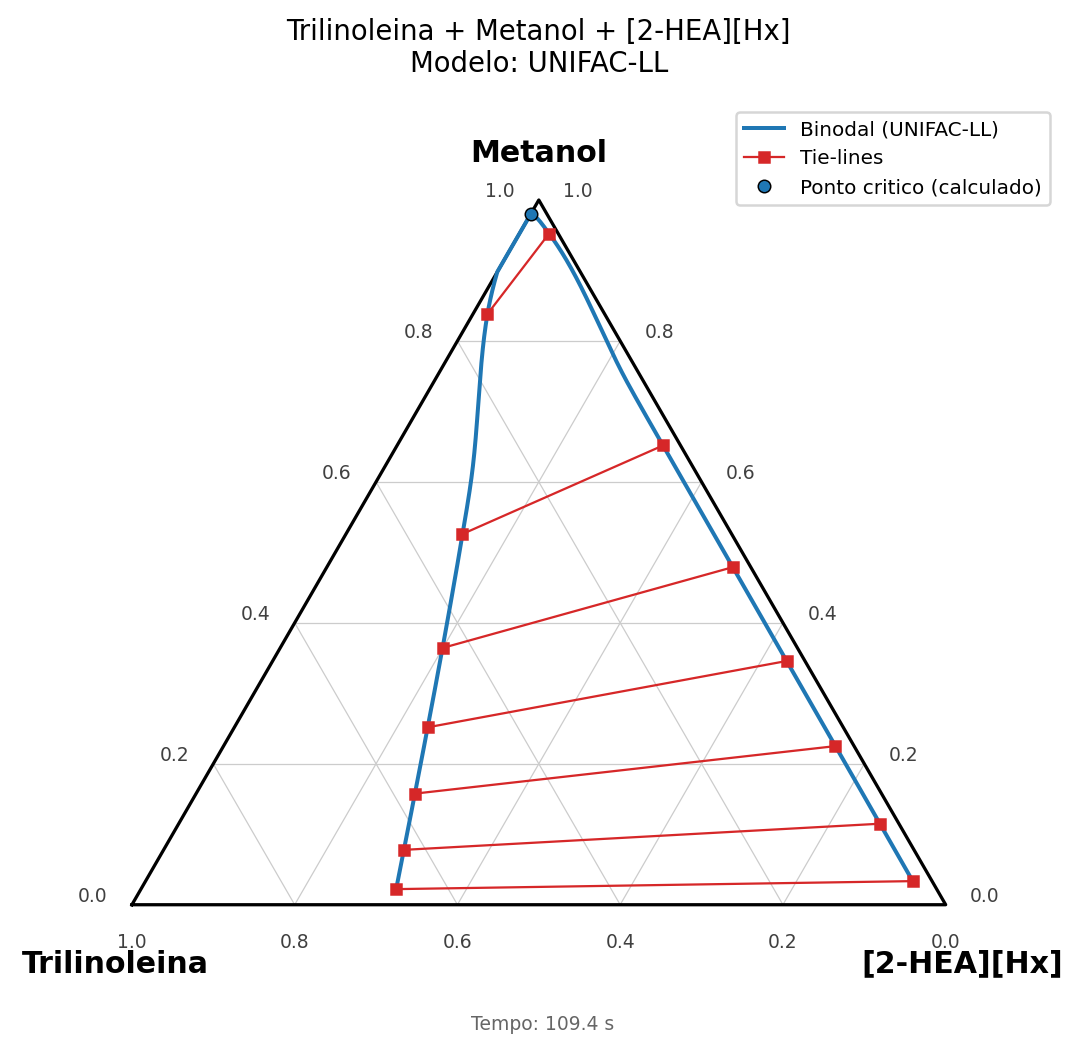
\includegraphics[width=0.4\textwidth]{imagens/ELL_Trilinoleina_Metanol_2_HEAHx_UNIFAC_LL.png}
\hfill
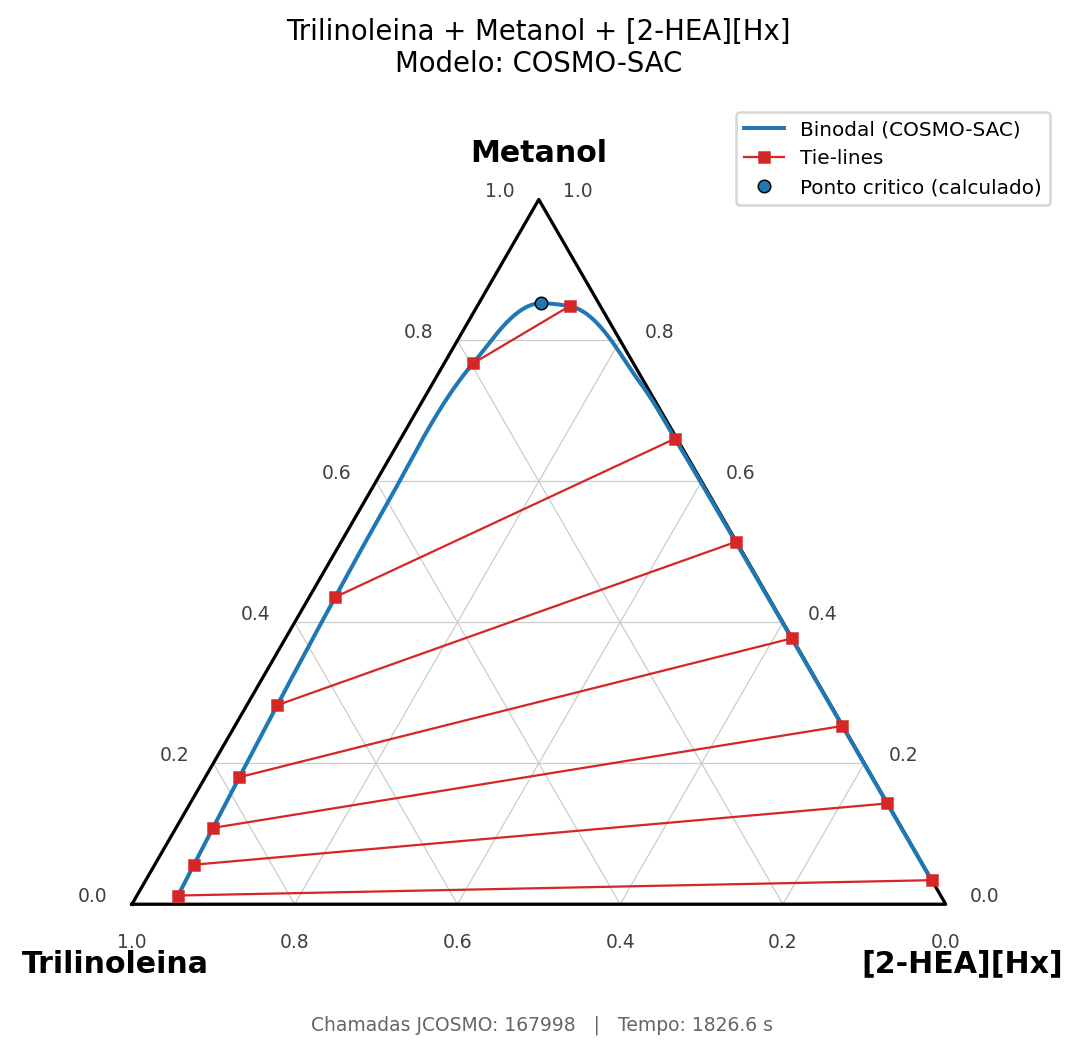
\includegraphics[width=0.4\textwidth]{imagens/ELL_Trilinoleina_Metanol_2_HEAHx_COSMO_SAC.png}
\caption{Trilinoleína + metanol + [2-HEA][Hx]: UNIFAC-LL (esquerda) e COSMO-SAC (direita)}
\label{fig:trilinoleina_metanol_2hea}
\end{figure}

\begin{figure}[H]
\centering
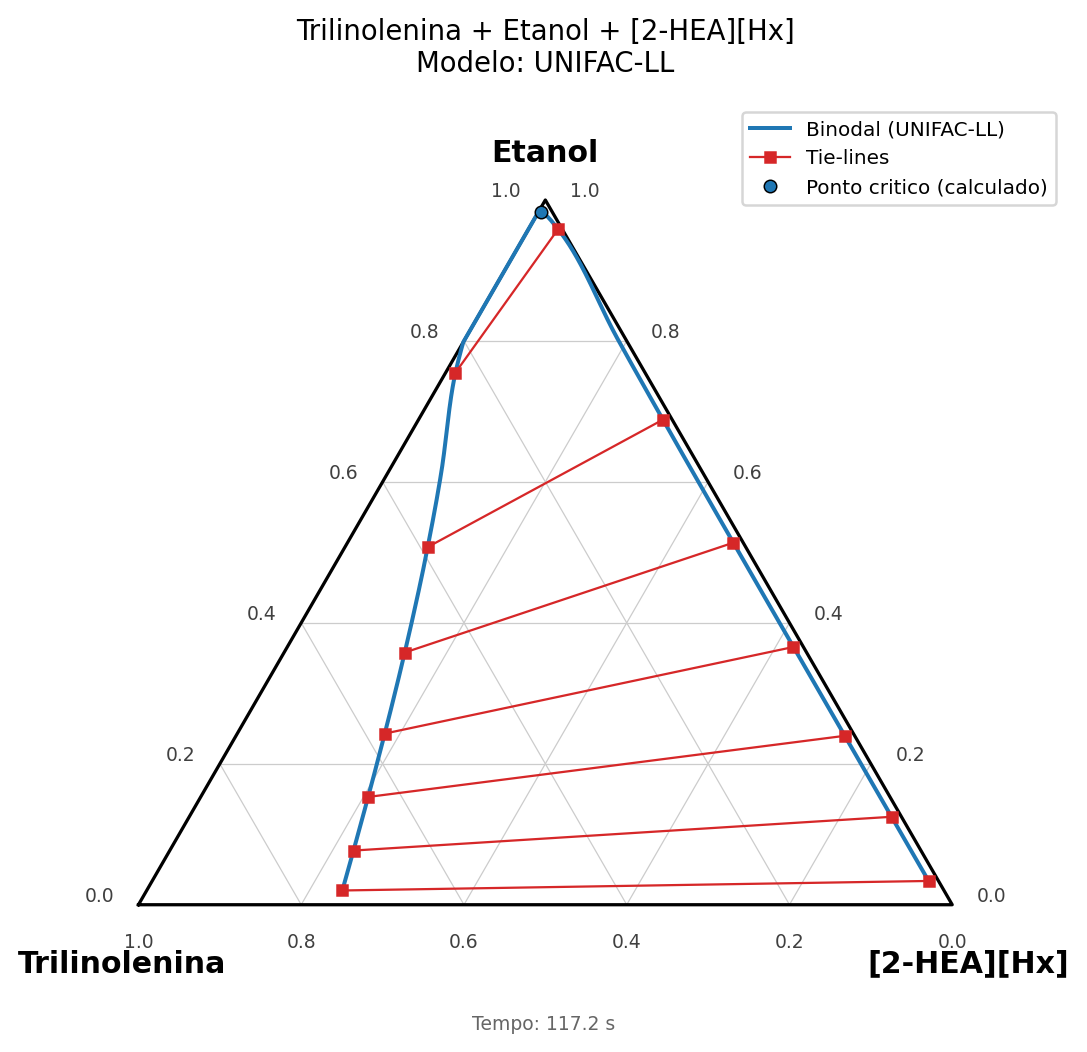
\includegraphics[width=0.4\textwidth]{imagens/ELL_Trilinolenina_Etanol_2_HEAHx_UNIFAC_LL.png}
\hfill
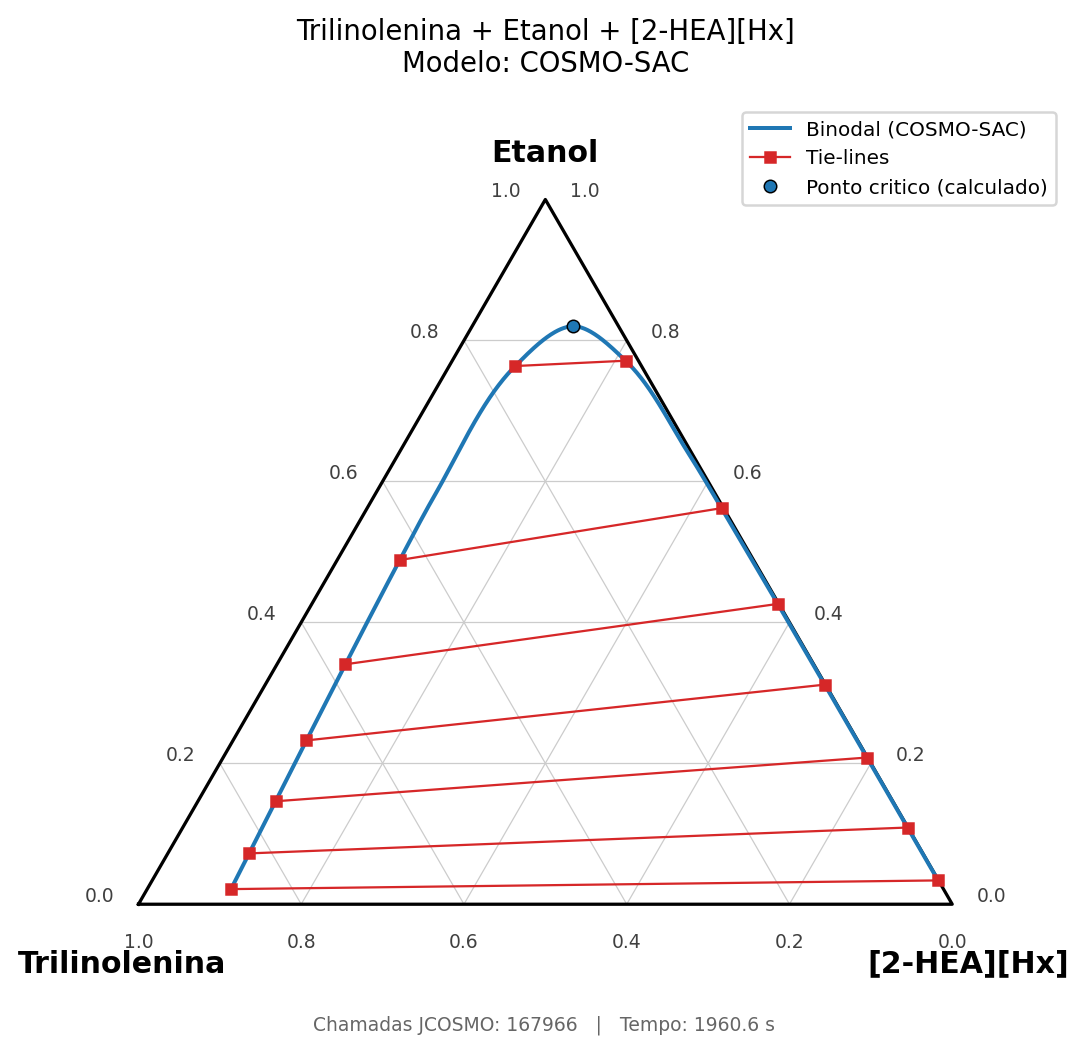
\includegraphics[width=0.4\textwidth]{imagens/ELL_Trilinolenina_Etanol_2_HEAHx_COSMO_SAC.png}
\caption{Trilinolenina + etanol + [2-HEA][Hx]: UNIFAC-LL (esquerda) e COSMO-SAC (direita)}
\label{fig:trilinolenina_etanol_2hea}
\end{figure}

\begin{figure}[H]
\centering
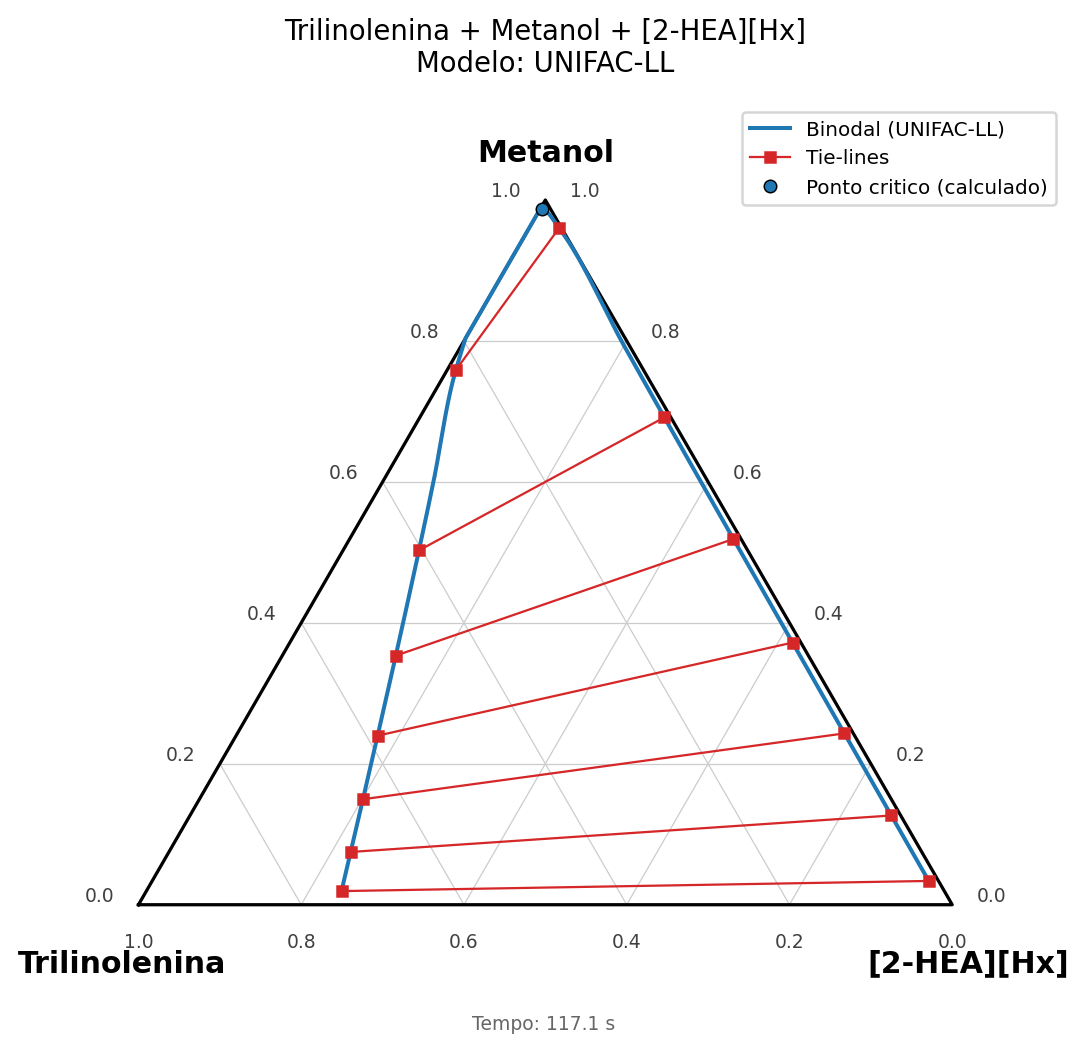
\includegraphics[width=0.4\textwidth]{imagens/ELL_Trilinolenina_Metanol_2_HEAHx_UNIFAC_LL.png}
\hfill
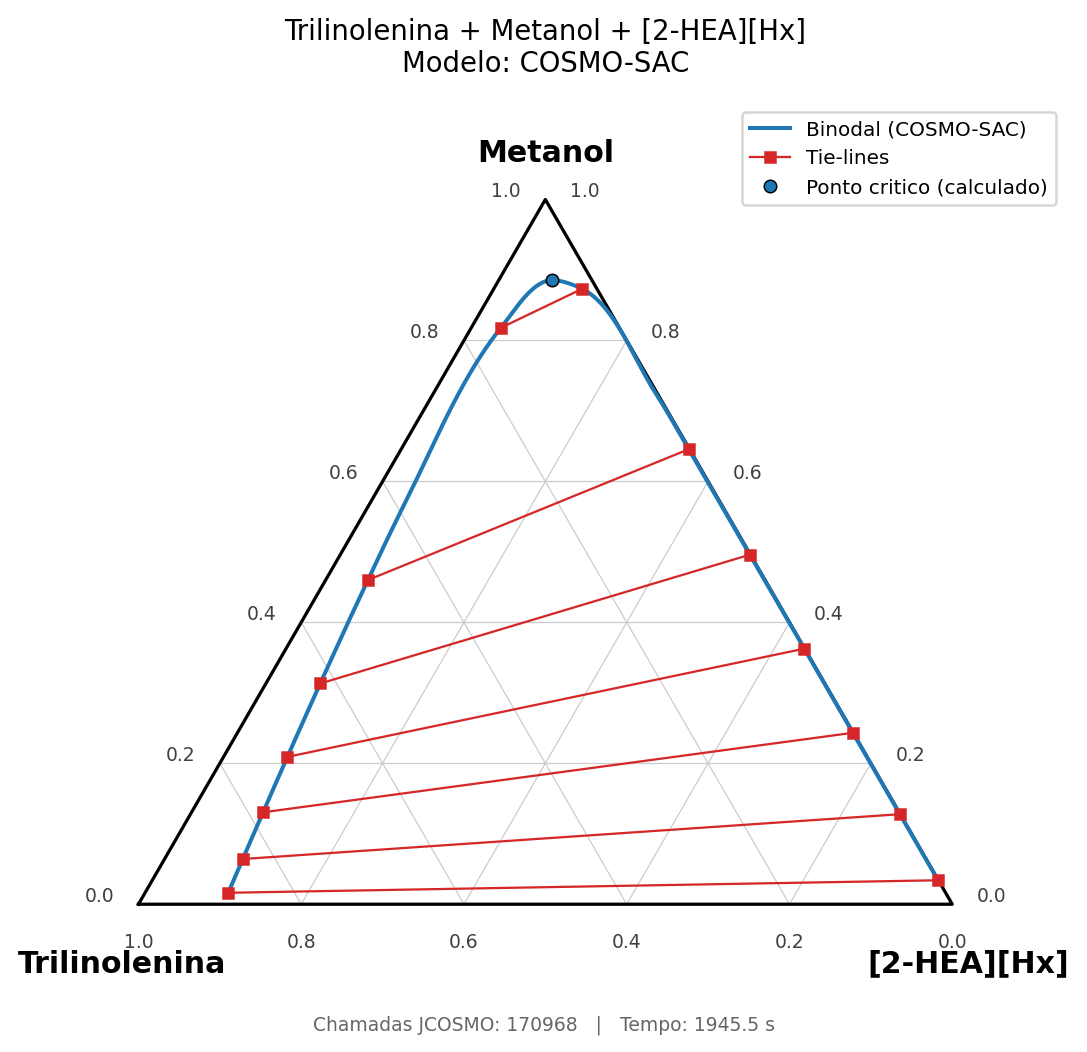
\includegraphics[width=0.4\textwidth]{imagens/ELL_Trilinolenina_Metanol_2_HEAHx_COSMO_SAC.png}
\caption{Trilinolenina + metanol + [2-HEA][Hx]: UNIFAC-LL (esquerda) e COSMO-SAC (direita)}
\label{fig:trilinolenina_metanol_2hea}
\end{figure}

Quanto à extensão da região bifásica, a área calculada pelo COSMO-SAC varia entre 0,3819 e 0,4564 nesses seis sistemas (média de 0,4214), faixa retomada adiante na comparação com os sistemas contendo [DETA][Hx] (Seção~\ref{subsec:resultados_deta}). A concordância entre os dois modelos, nesse conjunto, é de natureza qualitativa, pois ambos preveem o mesmo tipo de binodal e não divergem quanto à existência de duas fases líquidas, embora posicionem a curva de maneira distinta no espaço de composições. Tal distinção pode ser medida pela distância euclidiana entre os pontos críticos estimados por cada modelo para um mesmo sistema, que se situa entre 0,0616 e 0,3966 em fração molar (média de 0,1599), com o sistema \{trioleína + etanol\} destacando-se dos demais ao registrar a maior distância (0,3966) enquanto os outros cinco permanecem entre 0,0616 e 0,1621. Uma vez que o ponto crítico é obtido por extrapolação do encolhimento sucessivo da região instável (Seção~\ref{subsec:motor_termodinamico}), em vez de resolver-se diretamente a condição crítica, essas distâncias carregam a incerteza própria desse procedimento e devem ser lidas como ordem de grandeza da discrepância entre os modelos.

Considerando-se que os dois modelos partem de naturezas bastante distintas (contribuição de grupos, de um lado, e cálculo a priori a partir de perfis sigma, de outro), a coincidência quanto ao tipo de comportamento de fases sugere que a tendência à separação nos sistemas com [2-HEA][Hx] não depende da escolha de um modelo específico, ainda que a verificação dessa leitura dependa de dados experimentais indisponíveis para esses sistemas (Seção~\ref{sec:dados_validacao}).

Entre os três triglicerídeos, o resultado da trilinoleína deve ser lido com a ressalva já registrada na Seção~\ref{subsec:parametros_perfis}, visto que o enovelamento identificado em seu perfil sigma tende a superestimar a fração polar da molécula e, por conseguinte, sua afinidade com o álcool e com o líquido iônico. Como apenas o COSMO-SAC consome o perfil sigma comprometido, a formação de região bifásica também no UNIFAC-LL, que não depende dessa geometria, indica que o comportamento em si não decorre exclusivamente do artefato.

\subsection{Sistemas com [DETA][Hx]}
\label{subsec:resultados_deta}

Os sistemas que envolvem o líquido iônico prótico [DETA][Hx] apresentam um quadro distinto do anterior, no qual os dois modelos deixam de concordar sequer quanto à existência de duas fases líquidas. No UNIFAC-LL, nenhum dos seis sistemas apresentou binodal genuína, uma vez que os quatro casos com trioleína e trilinoleína convergiram diretamente para zero linhas de amarração, ou seja, o teste de estabilidade não identificou composição instável em toda a extensão do diagrama, enquanto os dois casos com trilinolenina produziram apenas quatro linhas, confinadas a uma faixa estreita próxima ao vértice do álcool puro (fração de trilinolenina inferior a 0,23 em ambas as fases). Não foi possível, portanto, construir a curva binodal para nenhum dos seis sistemas com [DETA][Hx] no UNIFAC-LL, e o resultado é registrado nesses termos, já que a ausência de composição instável identificada pelo teste de estabilidade é compatível tanto com uma fase única termodinamicamente estável quanto com uma falha de convergência do procedimento nas condições avaliadas.

O COSMO-SAC, em contrapartida, prevê binodal do tipo 1 em todos os seis, com número de linhas de amarração entre 327 e 370 (Tabela~\ref{tab:tielines_deta}), na mesma ordem de grandeza registrada para os sistemas com [2-HEA][Hx].

\begin{table}[htb]
\centering
\caption{Número de tie-lines calculadas para os sistemas com [DETA][Hx]}
\label{tab:tielines_deta}
\begin{tabular}{lcc}
\hline
Sistema & UNIFAC-LL & COSMO-SAC \\
\hline
Trioleína + Etanol      & 0 (curva não obtida) & 367 \\
Trioleína + Metanol     & 0 (curva não obtida) & 362 \\
Trilinoleína + Etanol   & 0 (curva não obtida) & 370 \\
Trilinoleína + Metanol  & 0 (curva não obtida) & 356 \\
Trilinolenina + Etanol  & 4 (insuficientes para a curva) & 334 \\
Trilinolenina + Metanol & 4 (insuficientes para a curva) & 344 \\
\hline
\end{tabular}
\end{table}

\begin{figure}[H]
\centering
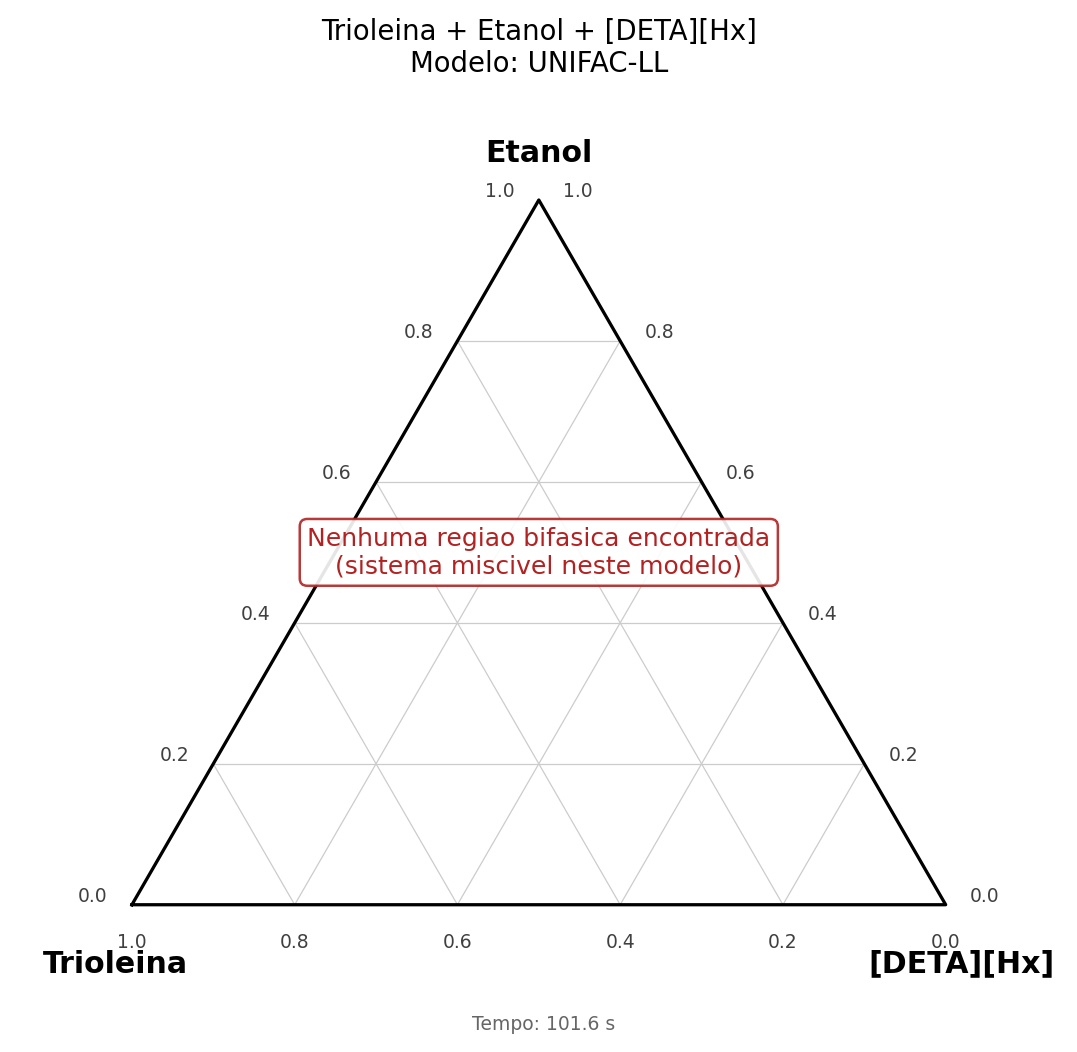
\includegraphics[width=0.4\textwidth]{imagens/ELL_Trioleina_Etanol_DETAHx_UNIFAC_LL.png}
\hfill
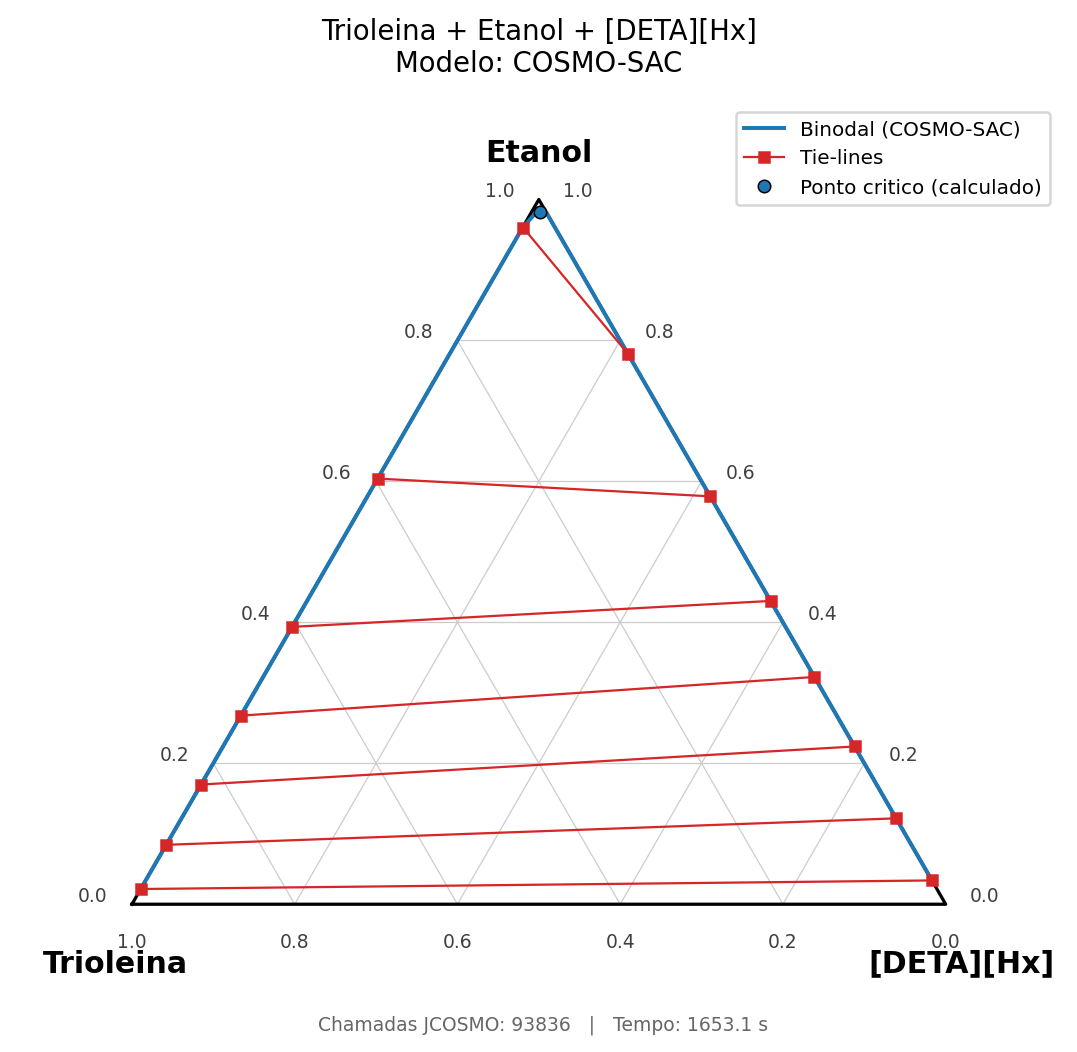
\includegraphics[width=0.4\textwidth]{imagens/ELL_Trioleina_Etanol_DETAHx_COSMO_SAC.png}
\caption{Trioleína + etanol + [DETA][Hx]: UNIFAC-LL (esquerda, curva não obtida) e COSMO-SAC (direita)}
\label{fig:trioleina_etanol_deta}
\end{figure}

\begin{figure}[H]
\centering
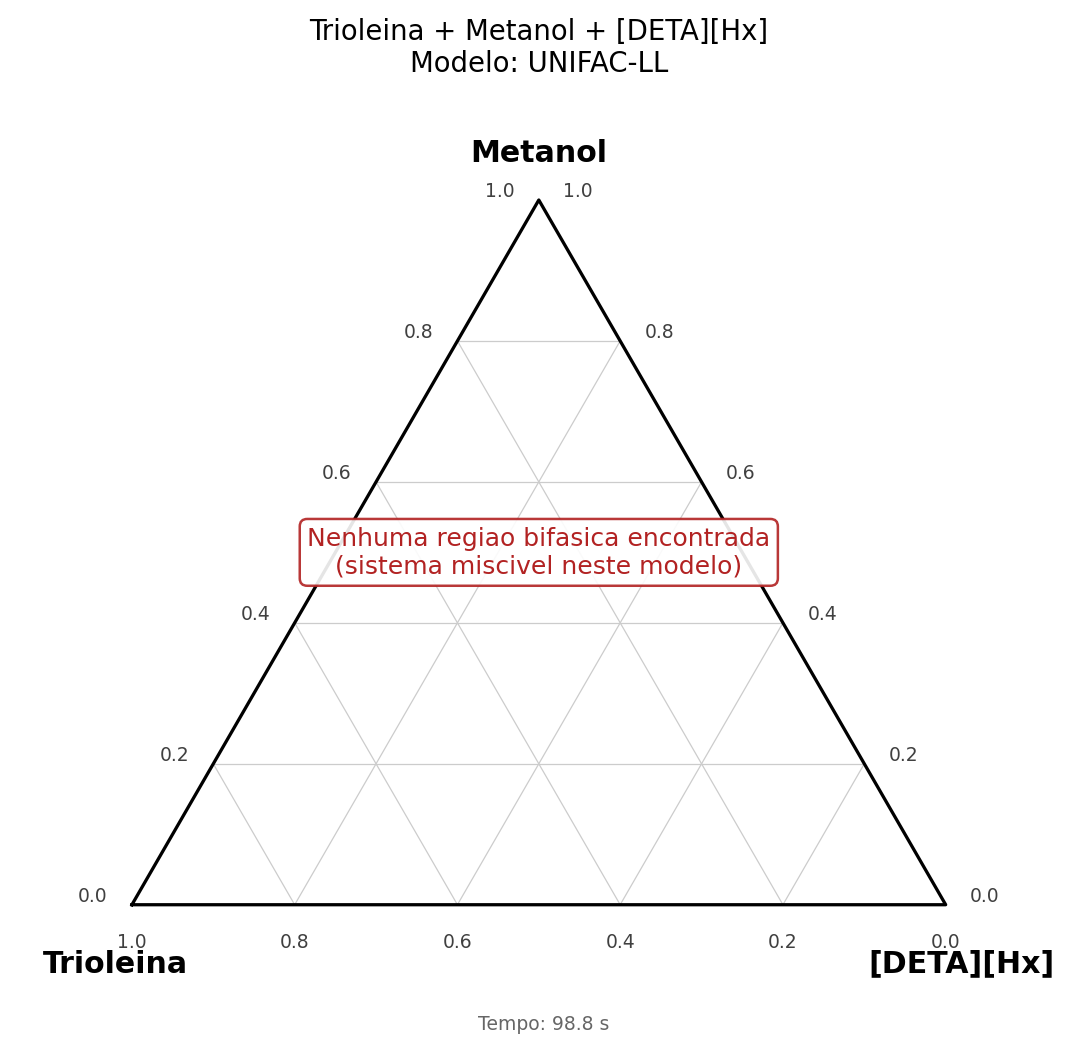
\includegraphics[width=0.4\textwidth]{imagens/ELL_Trioleina_Metanol_DETAHx_UNIFAC_LL.png}
\hfill
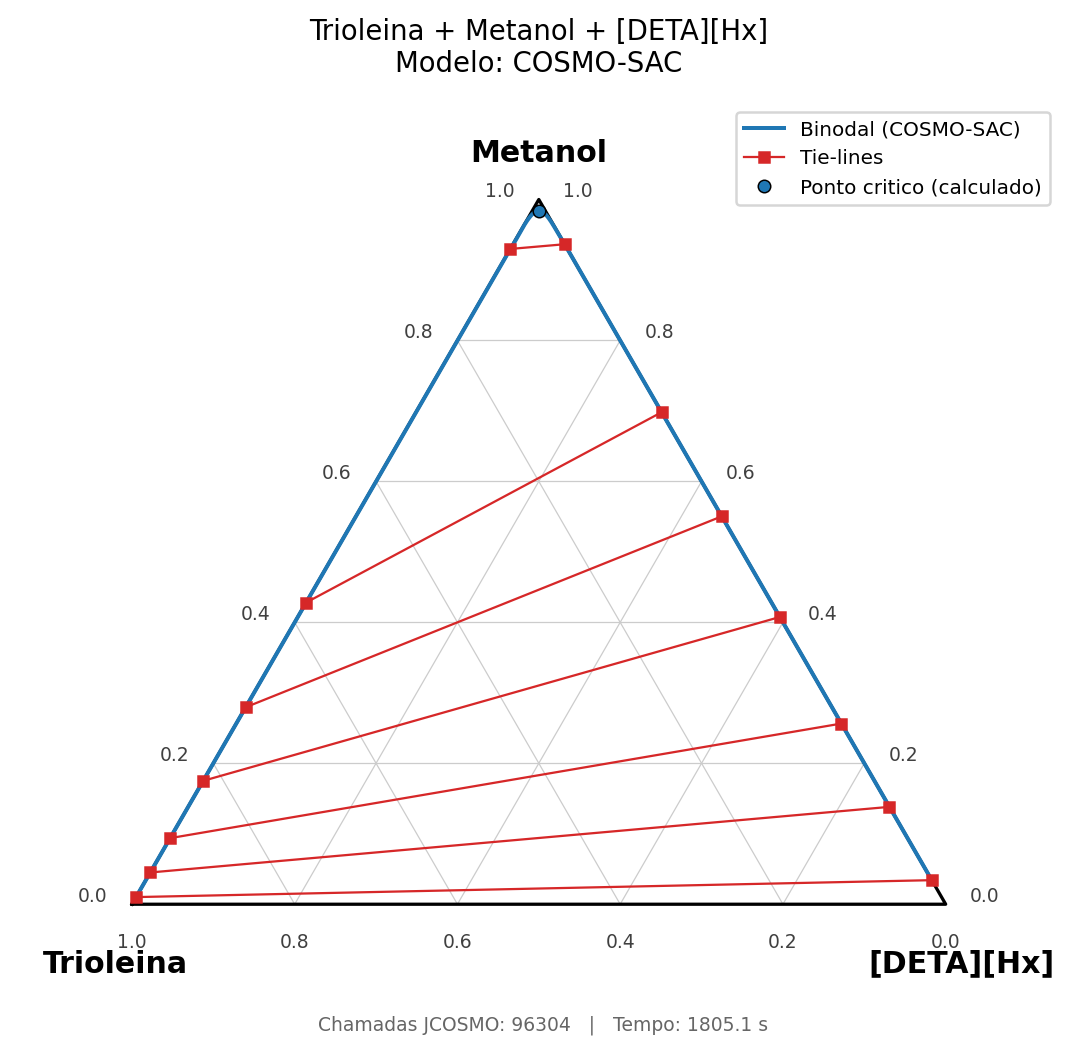
\includegraphics[width=0.4\textwidth]{imagens/ELL_Trioleina_Metanol_DETAHx_COSMO_SAC.png}
\caption{Trioleína + metanol + [DETA][Hx]: UNIFAC-LL (esquerda, curva não obtida) e COSMO-SAC (direita)}
\label{fig:trioleina_metanol_deta}
\end{figure}

\begin{figure}[H]
\centering
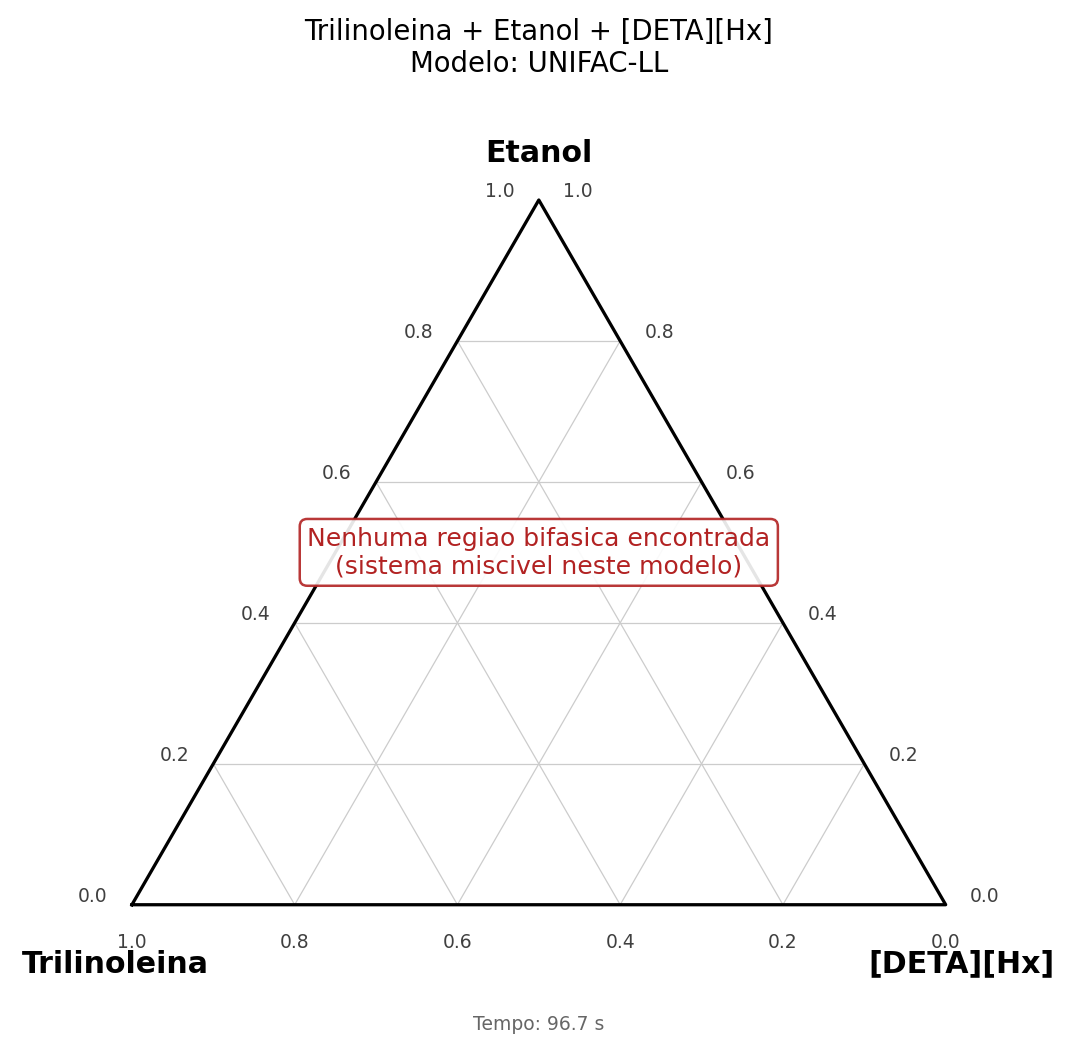
\includegraphics[width=0.4\textwidth]{imagens/ELL_Trilinoleina_Etanol_DETAHx_UNIFAC_LL.png}
\hfill
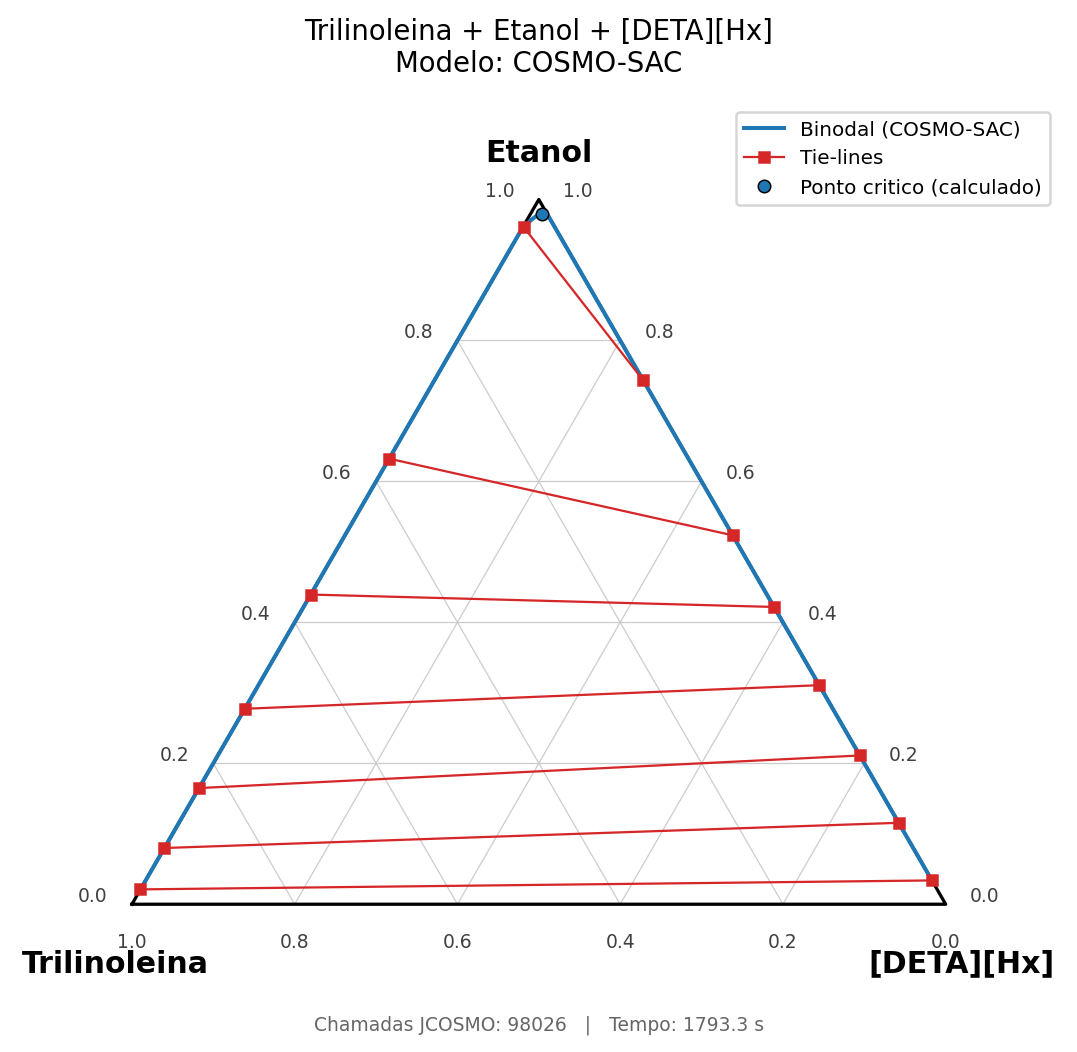
\includegraphics[width=0.4\textwidth]{imagens/ELL_Trilinoleina_Etanol_DETAHx_COSMO_SAC.png}
\caption{Trilinoleína + etanol + [DETA][Hx]: UNIFAC-LL (esquerda, curva não obtida) e COSMO-SAC (direita)}
\label{fig:trilinoleina_etanol_deta}
\end{figure}

\begin{figure}[H]
\centering
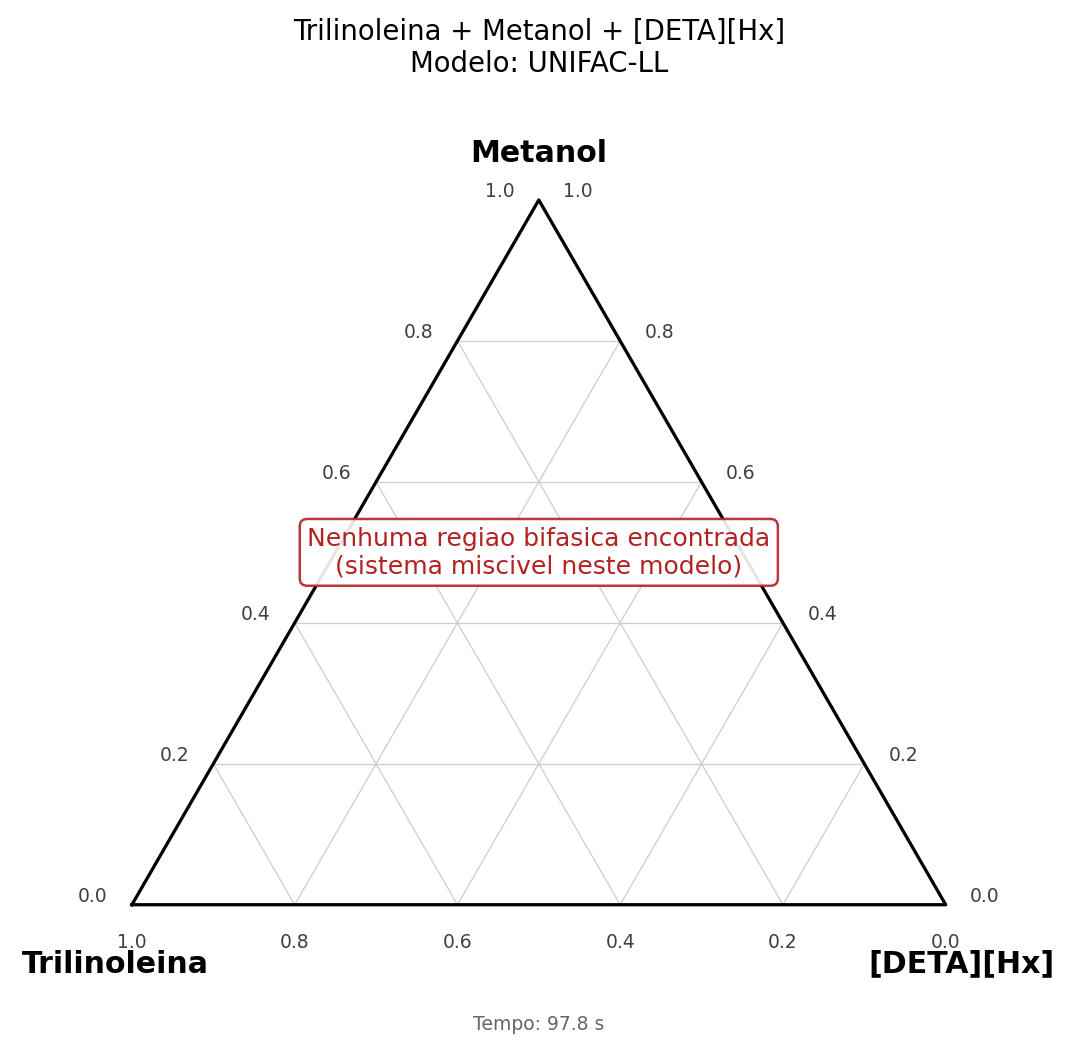
\includegraphics[width=0.4\textwidth]{imagens/ELL_Trilinoleina_Metanol_DETAHx_UNIFAC_LL.png}
\hfill
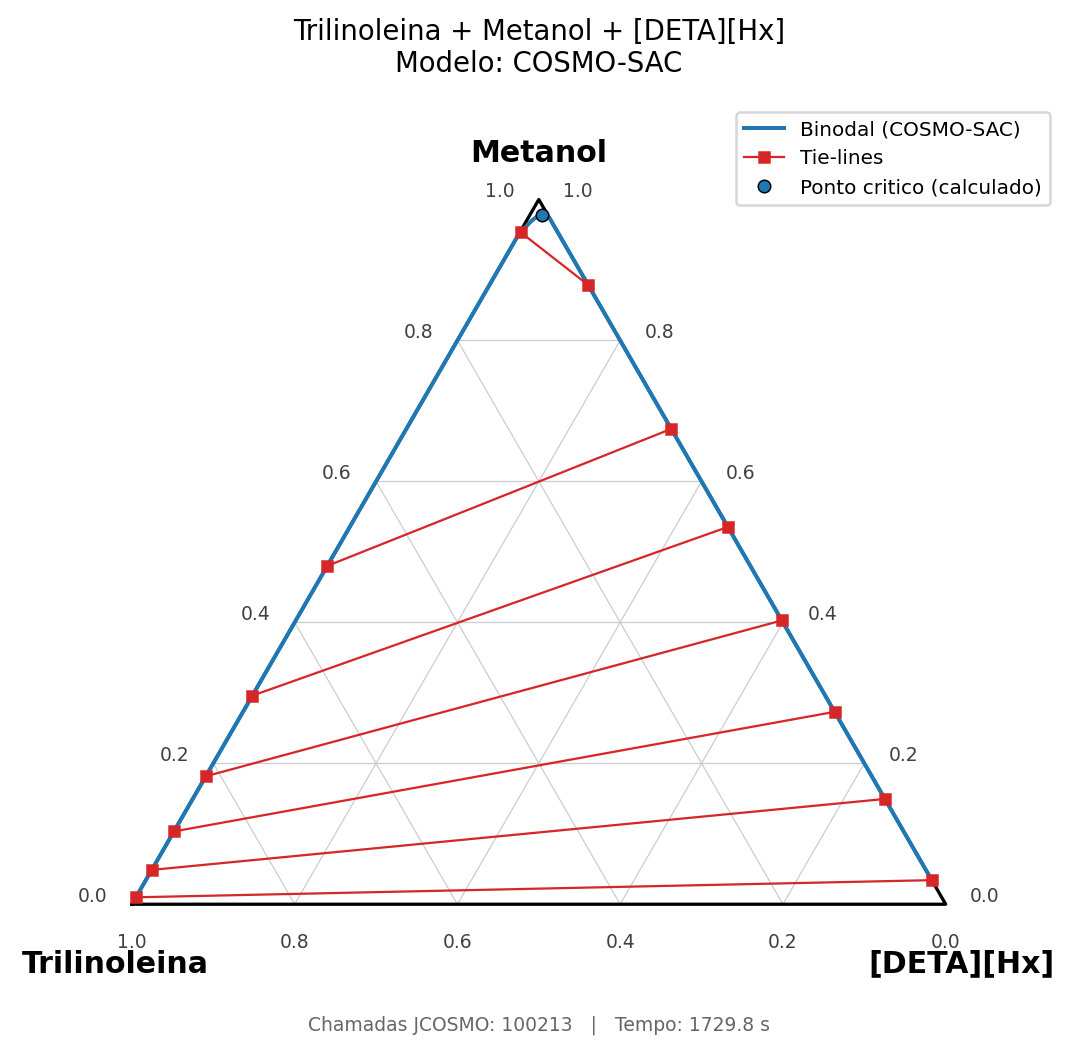
\includegraphics[width=0.4\textwidth]{imagens/ELL_Trilinoleina_Metanol_DETAHx_COSMO_SAC.png}
\caption{Trilinoleína + metanol + [DETA][Hx]: UNIFAC-LL (esquerda, curva não obtida) e COSMO-SAC (direita)}
\label{fig:trilinoleina_metanol_deta}
\end{figure}

\begin{figure}[H]
\centering
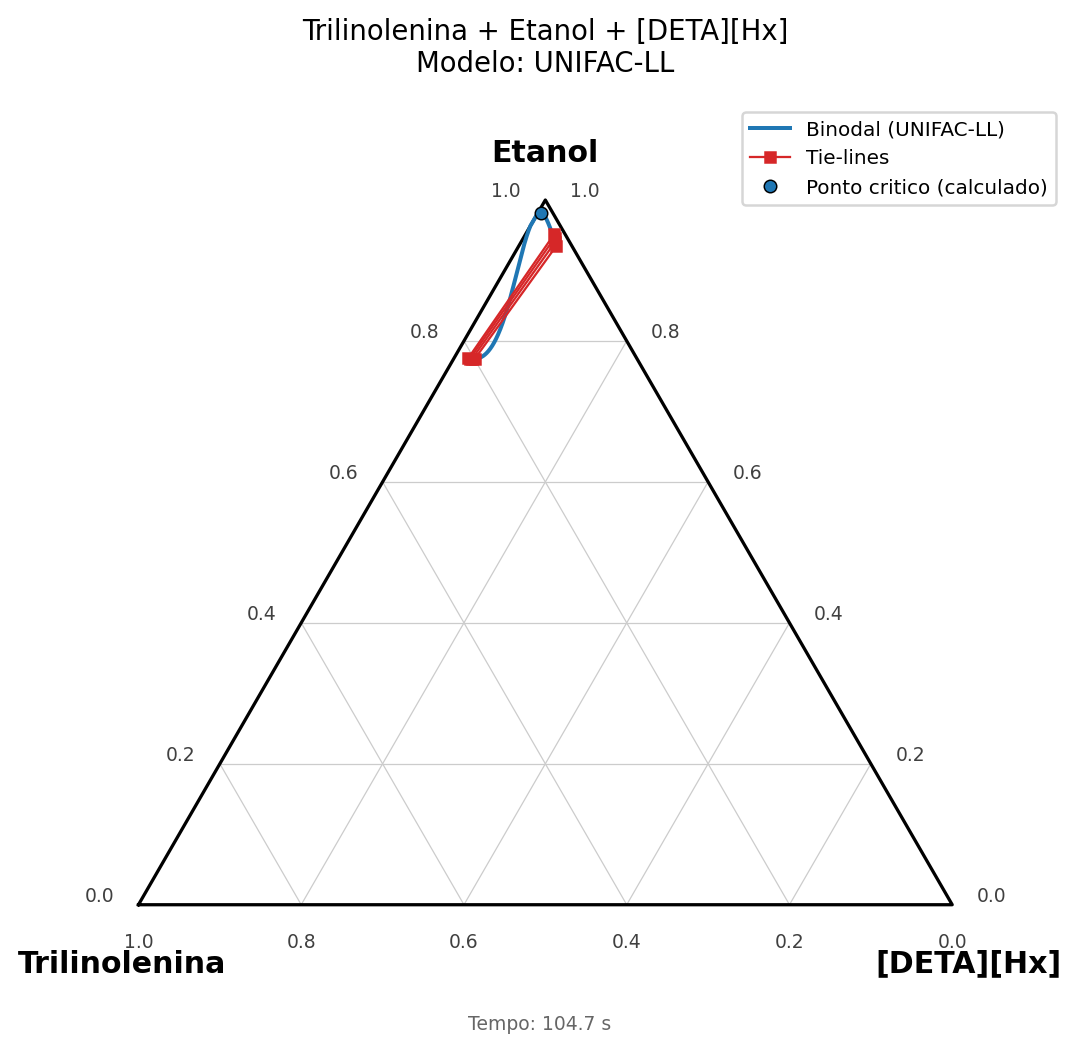
\includegraphics[width=0.4\textwidth]{imagens/ELL_Trilinolenina_Etanol_DETAHx_UNIFAC_LL.png}
\hfill
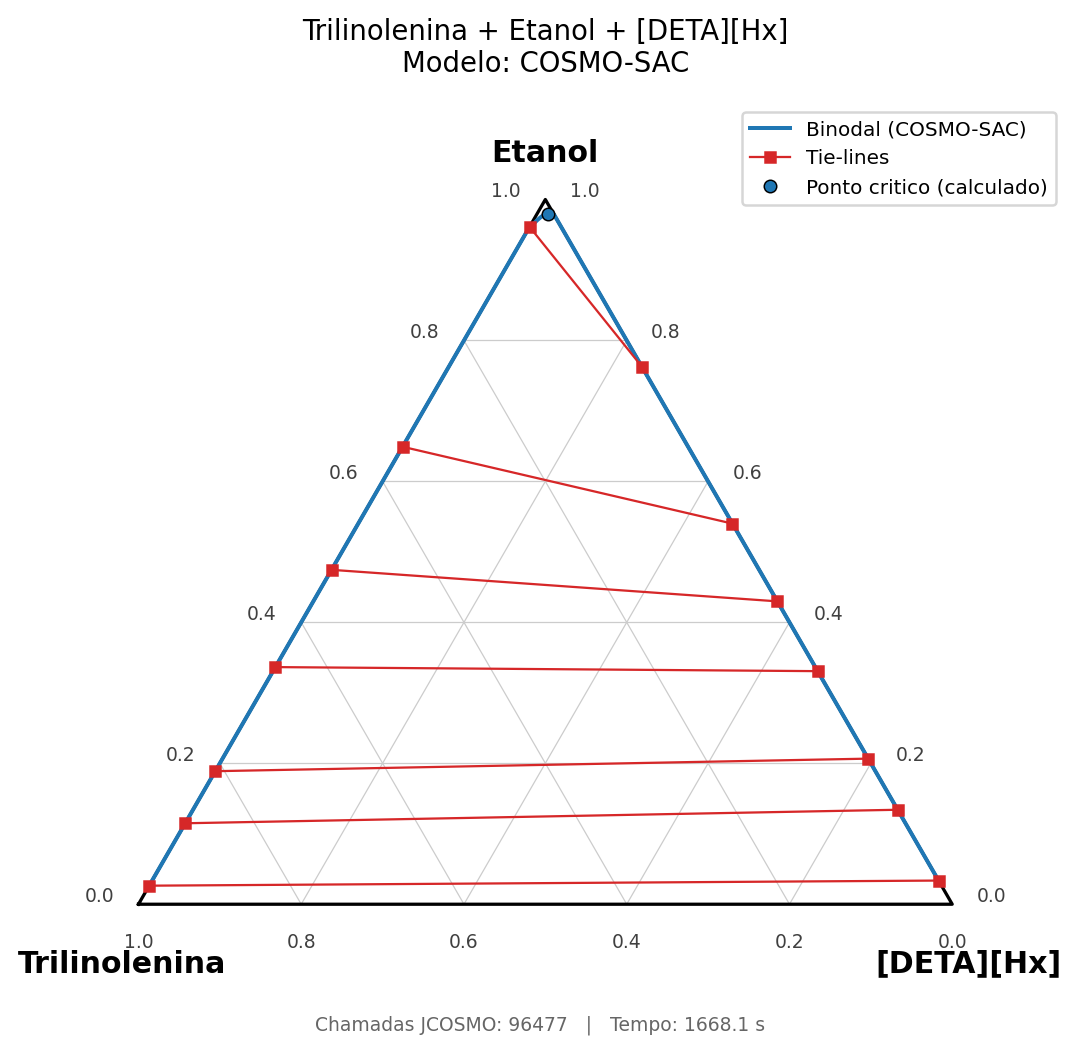
\includegraphics[width=0.4\textwidth]{imagens/ELL_Trilinolenina_Etanol_DETAHx_COSMO_SAC.png}
\caption{Trilinolenina + etanol + [DETA][Hx]: o UNIFAC-LL (esquerda) produz apenas quatro tie-lines confinadas ao vértice do álcool, insuficientes para o traçado da curva; o COSMO-SAC (direita) prevê uma binodal completa}
\label{fig:trilinolenina_etanol_deta}
\end{figure}

\begin{figure}[H]
\centering
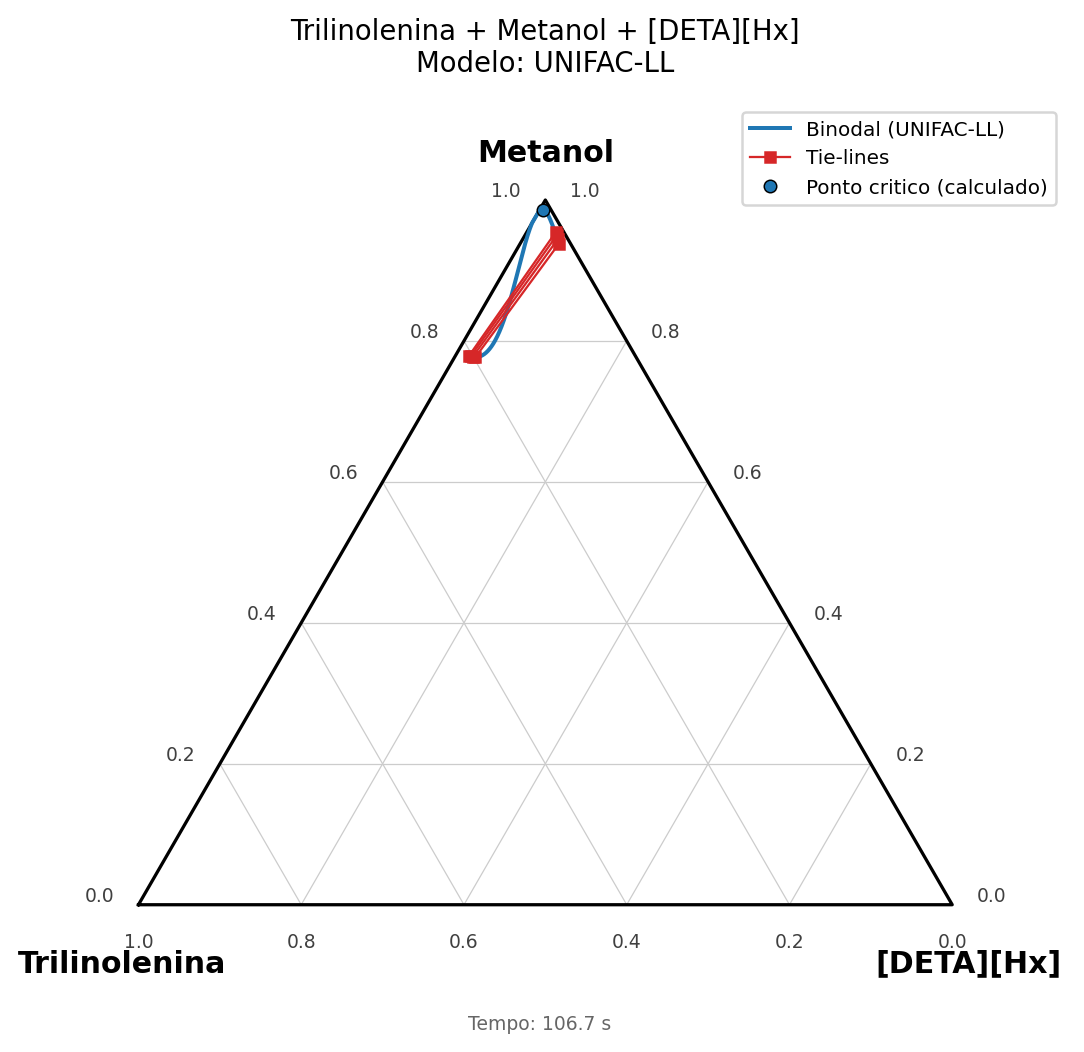
\includegraphics[width=0.4\textwidth]{imagens/ELL_Trilinolenina_Metanol_DETAHx_UNIFAC_LL.png}
\hfill
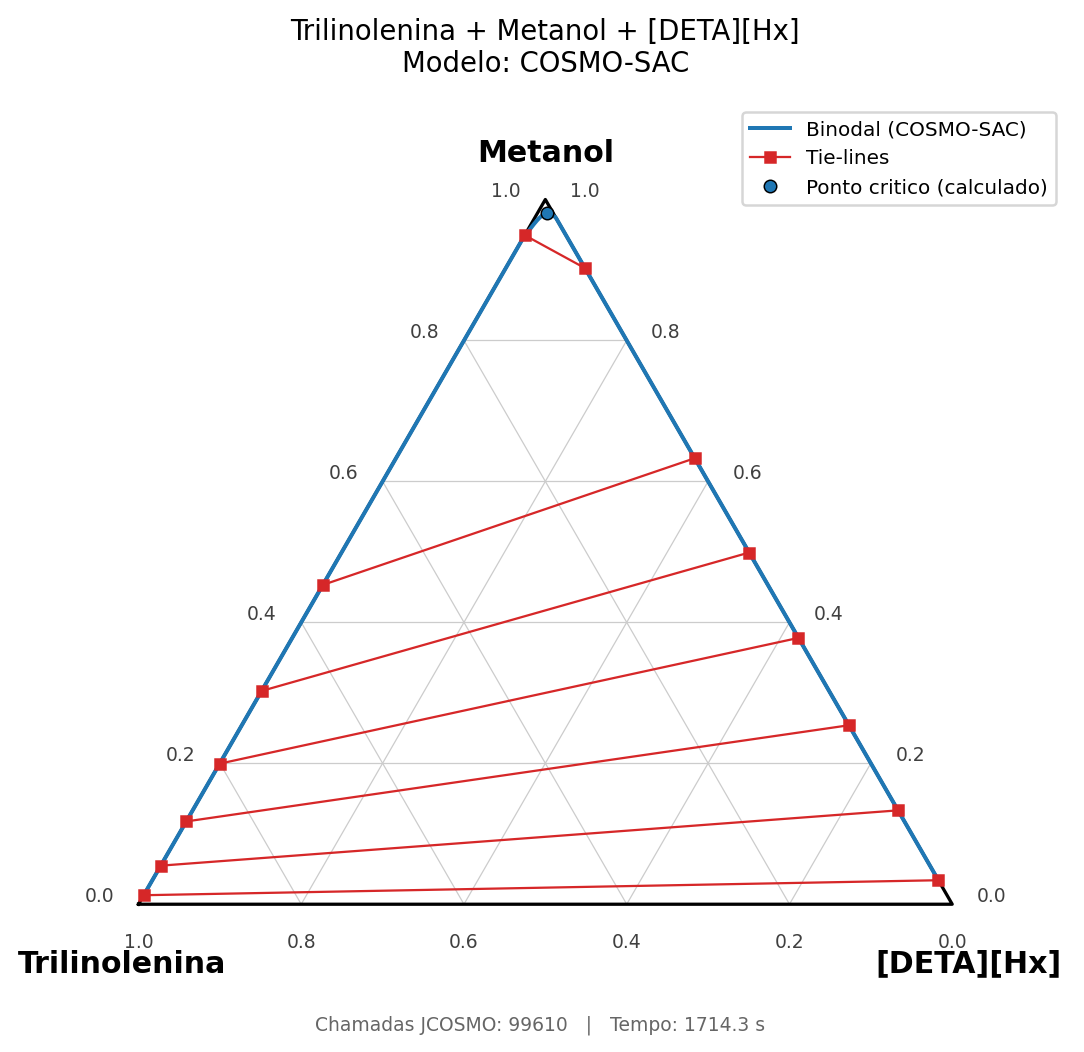
\includegraphics[width=0.4\textwidth]{imagens/ELL_Trilinolenina_Metanol_DETAHx_COSMO_SAC.png}
\caption{Trilinolenina + metanol + [DETA][Hx]: o UNIFAC-LL (esquerda) produz apenas quatro tie-lines confinadas ao vértice do álcool, insuficientes para o traçado da curva; o COSMO-SAC (direita) prevê uma binodal completa}
\label{fig:trilinolenina_metanol_deta}
\end{figure}

A área da região bifásica prevista pelo COSMO-SAC varia entre 0,4659 e 0,4758 nesses seis sistemas (média de 0,4713), portanto acima da média de 0,4214 obtida para os sistemas equivalentes com [2-HEA][Hx] (Seção~\ref{subsec:resultados_2hea}), e à diferença de magnitude soma-se uma diferença de dispersão que merece atenção: enquanto com [2-HEA][Hx] a área percorre uma faixa de aproximadamente 0,07 conforme o triglicerídeo e o álcool empregados (de 0,3819 a 0,4564), com [DETA][Hx] essa faixa se reduz a cerca de 0,01. Sendo assim, na predição do COSMO-SAC, a identidade do triglicerídeo e a do álcool influenciam pouco a extensão da região bifásica quando o [DETA][Hx] está presente, o que sugere que esse líquido iônico prótico domina o comportamento de fases do sistema, ao contrário do que se observa com o [2-HEA][Hx]. O ponto crítico acompanha esse quadro, situando-se consistentemente próximo ao vértice do álcool puro, com fração molar de álcool entre 0,852 e 0,933 e fração de triglicerídeo entre apenas 0,019 e 0,035, o que corresponde a uma região monofásica estável restrita a composições dominadas por álcool quase puro.

A divergência entre os modelos é, nesse conjunto, de natureza categórica, pois eles discordam quanto à própria ocorrência da separação de fases e não apenas quanto ao tamanho da região bifásica. Ela tampouco admite quantificação simétrica, uma vez que do lado do UNIFAC-LL não há região bifásica da qual extrair área ou ponto crítico, o que inviabiliza tanto o cálculo de uma distância entre pontos críticos (como se fez na Seção~\ref{subsec:resultados_2hea}) quanto qualquer forma de valor intermediário entre as duas predições, já que a existência de duas fases líquidas é propriedade qualitativa do sistema e não grandeza que admita interpolação.

Duas observações de plausibilidade cabem ao caso, uma para cada modelo, sem que nenhuma delas resolva a divergência. Do lado do COSMO-SAC, uma região bifásica que ocupa perto de metade do simplex, com ponto crítico tão próximo ao vértice do álcool, implica desestabilização da mistura mesmo em frações muito baixas de triglicerídeo, previsão extrema mas não implausível, visto que cátions poliprotonados são associados na literatura a efeitos de \textit{salting-out} desproporcionais ao seu tamanho molecular, mecanismo retomado na Seção~\ref{subsec:salting_in_out}. Do lado do UNIFAC-LL, a ausência de região bifásica nos seis sistemas depende dos quatro parâmetros de interação preenchidos por completamento de matriz (Seção~\ref{subsec:parametros_perfis}), aplicados aqui a uma combinação (triglicerídeo C57 com cátion amônio triprotonado de cadeia estendida) mais distante da base de treinamento do que a correspondente com [2-HEA][Hx], o que torna a predição menos ancorada, embora não a invalide por si só. Ambas as observações são retomadas na síntese ao final do capítulo (Seção~\ref{subsec:sintese}).

\subsection{Efeito do álcool}
\label{subsec:efeito_alcool}

Mantendo-se fixos o triglicerídeo e o líquido iônico prótico, a substituição do etanol pelo metanol amplia a região de imiscibilidade nos sistemas em que foi possível construir a curva binodal, tendência que já se manifesta no par binário triglicerídeo-álcool, isolado do restante do sistema, uma vez que o coeficiente de atividade em diluição infinita calculado pelo COSMO-SAC para a trioleína em etanol é de 2,61, contra 3,76 em metanol, desvio positivo apreciavelmente mais forte. Esse resultado é coerente com o tamanho da cadeia alquílica de cada álcool, visto que o metanol, por possuir um único átomo de carbono, apresenta superfície molecular proporcionalmente mais dominada pela hidroxila polar do que o etanol, o que reduz sua afinidade com as longas cadeias apolares do triglicerídeo.

A comparação nos diagramas ternários completos abrange nove pares etanol/metanol, correspondentes aos seis pares com [2-HEA][Hx] (três triglicerídeos, em cada um dos dois modelos) somados aos três pares com [DETA][Hx] no COSMO-SAC, ficando de fora os sistemas com [DETA][Hx] no UNIFAC-LL, para os quais não se obteve curva binodal (Seção~\ref{subsec:resultados_deta}) e, por conseguinte, não há área nem ponto crítico a comparar.

Duas medidas apontam no mesmo sentido nesse conjunto. A área da região bifásica é maior com metanol nos nove pares, com aumento entre 1,6\% e 34\% e média em torno de 12\%, ao passo que o ponto crítico desloca-se em direção ao vértice do álcool puro em oito dos nove pares, apresentando fração de álcool superior à do par equivalente com etanol. Considerando-se que essas duas grandezas são obtidas por procedimentos independentes entre si (integração da curva binodal, no primeiro caso, e extrapolação do encolhimento da região instável, no segundo), a convergência entre elas reforça a leitura de que o efeito observado provém do álcool empregado, e dificilmente do método de cálculo.

O número de linhas de amarração acompanha essa tendência nos seis sistemas com [2-HEA][Hx] (Tabela~\ref{tab:tielines_2hea}), nos quais a contagem com metanol supera a com etanol nos dois modelos, mas o mesmo não se verifica nos três sistemas com [DETA][Hx] no COSMO-SAC, em que a contagem cai de 367 para 362 na trioleína e de 370 para 356 na trilinoleína, aumentando apenas na trilinolenina, de 334 para 344 (Tabela~\ref{tab:tielines_deta}). Levando em consideração que a contagem é um indicador da extensão da região bifásica e não uma medida direta dela, conforme observado na abertura desta seção, e que justamente nesses sistemas a área varia numa faixa muito estreita (Seção~\ref{subsec:resultados_deta}), essa discordância pontual não contradiz o que indicam a área e o ponto crítico, embora deva ser registrada em vez de descrever-se a tendência como uniforme.

A diferença entre etanol e metanol aqui caracterizada refere-se ao comportamento de fases a 298,15~K, sem estender-se ao desempenho de cada álcool na reação de transesterificação, no qual entram fatores alheios ao equilíbrio líquido-líquido, como a reatividade do alcóxido correspondente e a estequiometria empregada, de modo que a escolha entre os dois álcoois em processo não decorre diretamente do que se observa nesta seção.

\subsection{Efeito do grau de insaturação}
\label{subsec:insaturacao}

Os três triglicerídeos estudados diferem entre si apenas pelo número de ligações duplas por cadeia graxa, mantendo-se fixo o número de carbonos por cadeia (C18), sendo a trioleína formada por três cadeias monoinsaturadas de ácido oleico, a trilinoleína por três cadeias diinsaturadas de ácido linoleico e a trilinolenina por três cadeias triinsaturadas de ácido linolênico. Cada ligação dupla adicional introduz uma região de maior densidade eletrônica ao longo da cadeia, associada aos elétrons $\pi$ deslocalizados, e reduz a flexibilidade conformacional nesse ponto, pois a geometria planar em torno da ligação dupla impede a livre rotação característica das ligações simples vizinhas, e ambas as alterações modificam discretamente a polarizabilidade da molécula e a distribuição de carga superficial capturada pelo perfil sigma, o que justifica examinar se essa variação estrutural se reflete no comportamento de fases.

A comparação mais controlada disponível é entre trioleína e trilinolenina, os dois triglicerídeos cujos perfis sigma se verificaram geometricamente saudáveis (Seção~\ref{subsec:parametros_perfis}), excluindo-se a trilinoleína pela ressalva do enovelamento. No COSMO-SAC, essa comparação abrange quatro pares, correspondentes às quatro combinações de álcool (etanol e metanol) e líquido iônico prótico ([2-HEA][Hx] e [DETA][Hx]), ao passo que no UNIFAC-LL abrange apenas dois, os pares com [2-HEA][Hx], visto que não se obteve curva binodal para os sistemas com [DETA][Hx] (Seção~\ref{subsec:resultados_deta}), assimetria que convém ter em conta ao ler os resultados adiante.

Nos dois pares disponíveis, o UNIFAC-LL registra aumento da área da região bifásica da trioleína para a trilinolenina, de 66\% no par com etanol e 27\% no par com metanol, enquanto nos quatro pares do COSMO-SAC as áreas resultam praticamente iguais ou ligeiramente menores para a trilinolenina, com variações de $-13\%$, $-9\%$, $-0{,}5\%$ e $-0{,}3\%$. Dois desses quatro valores são de magnitude comparável à incerteza esperada do próprio procedimento de cálculo da área, obtida por integração poligonal sobre as extremidades das linhas de amarração, de modo que o resultado do COSMO-SAC é mais bem descrito como ausência de efeito consistente da insaturação do que como inversão da tendência registrada pelo UNIFAC-LL.

Essa diferença é coerente com a forma como cada modelo representa a insaturação, pois no UNIFAC-LL cada ligação dupla substitui dois grupos \ce{CH2} por um grupo \ce{CH=CH}, alteração discreta na contagem de grupos que se propaga diretamente aos parâmetros $R_k$, $Q_k$ e às interações do grupo C=C, ao passo que no COSMO-SAC a insaturação aparece apenas como uma modulação suave da distribuição de carga superficial da cadeia, sem descontinuidade equivalente. A divergência observada é, portanto, compatível com a estrutura de cada modelo, sem que se possa atribuir maior correção a qualquer das duas representações.

Por conseguinte, a afirmação de que o grau de insaturação altera a miscibilidade dos sistemas estudados precisa vir acompanhada da ressalva de que a direção e a magnitude dessa alteração dependem do modelo empregado, ao contrário do que se observou para o efeito do álcool (Seção~\ref{subsec:efeito_alcool}), no qual as duas medidas independentes apontaram no mesmo sentido nos dois modelos.

A trilinoleína, embora se situe entre as outras duas em número de insaturações, não pode ser incluída nessa comparação com a mesma confiança, pois o enovelamento identificado em seu perfil sigma introduz um viés de superestimação de polaridade que se sobrepõe, e possivelmente mascara, o efeito da insaturação sobre a predição do COSMO-SAC, de modo que não é possível, a partir dos dados deste trabalho, separar quanto da área calculada reflete o grau de insaturação da molécula e quanto reflete a geometria comprometida. Essa ressalva não se aplica ao UNIFAC-LL, que não consome perfil sigma e para o qual a trilinoleína é descrita pela mesma contagem de grupos das demais.

\subsection{Sistemas sem curva binodal obtida}
\label{subsec:casos_sem_separacao}

Nem todos os sistemas avaliados resultaram em curva binodal, e reúnem-se aqui os casos em que isso não ocorreu, junto de um caso que produziu curva mas carrega ressalva relevante. Quando a varredura da grade não identifica composições instáveis, ou identifica um número insuficiente delas para o traçado da curva, registra-se que não foi possível construir a binodal naquelas condições, distinção que não é de forma, uma vez que a ausência de composição instável identificada pelo teste de estabilidade é compatível tanto com uma fase única termodinamicamente estável quanto com uma falha de convergência do procedimento, e os dados deste trabalho não permitem separar as duas hipóteses.

Os dois ácidos graxos livres avaliados, o oleico e o linoleico, correspondentes às cadeias graxas da trioleína e da trilinoleína, não produziram região de instabilidade em nenhuma das combinações testadas com álcool e líquido iônico prótico, de modo que não se obteve curva binodal para nenhum desses sistemas. Registre-se, contudo, que esses resultados provêm de execuções exploratórias, anteriores à consolidação da fila de cálculo empregada nos demais sistemas deste capítulo, e que a exportação formal no mesmo padrão dos demais não foi realizada dentro do escopo deste trabalho, razão pela qual os sistemas com ácido graxo livre figuram aqui como registro de execução, sem o mesmo estatuto dos sistemas com triglicerídeo.

Uma diferença estrutural entre o ácido graxo livre e o triglicerídeo correspondente é, ainda assim, digna de nota, e é retomada na Seção~\ref{subsec:efeito_esterico}. Enquanto as três cadeias esterificadas ao glicerol impõem ao triglicerídeo volume molecular e impedimento estérico consideráveis, o ácido graxo livre expõe um único grupo carboxila terminal (COOH), livre de vizinhança apolar que dispute o mesmo espaço, e portanto disponível para formar ligação de hidrogênio direta com a rede de amônio e carboxilato do líquido iônico. Tal diferença é consistente com a literatura de desacidificação de óleos vegetais que emprega líquidos iônicos de amônio como agente extrator, na qual o mesmo mecanismo é reportado como força motriz da extração, embora se trate de leitura estrutural plausível cuja verificação dependeria dos resultados computacionais que não foram consolidados.

Os dois sistemas de trilinolenina com [DETA][Hx] no UNIFAC-LL (Seção~\ref{subsec:resultados_deta}) apresentam situação diferente, pois a varredura identificou composições instáveis em número reduzido, quatro linhas de amarração com fração de trilinolenina inferior a 0,23 em ambas as fases, confinadas a uma faixa estreita próxima ao vértice do álcool puro. Um conjunto dessa dimensão não permite o traçado de uma curva binodal nem a estimativa do ponto crítico, e a proximidade dessas composições ao limite de estabilidade numérica do algoritmo de flash, combinada à sensibilidade do resultado à malha de composições inicial, desaconselha atribuir significado físico a linhas isoladas nessa região, sem que isso equivalha a afirmar que a região seja necessariamente estável. Implementou-se no código um filtro de número mínimo de linhas de amarração, que identifica automaticamente essa situação e a sinaliza como resultado não conclusivo, de modo que as tabelas deste capítulo já refletem tal depuração.

Já a trilinoleína produziu curva binodal em todos os sistemas avaliados, e a ressalva que a acompanha recai sobre a magnitude do resultado. Conforme discutido na Seção~\ref{subsec:parametros_perfis} e retomado nas Seções~\ref{subsec:resultados_2hea} e~\ref{subsec:insaturacao}, o perfil sigma dessa molécula apresenta conformação enovelada em vez de estendida, o que eleva sua fração polar superficial e tende a superestimar a afinidade calculada com o álcool e com o líquido iônico no COSMO-SAC. Sendo assim, a extensão da região bifásica obtida para a trilinoleína nesse modelo permanece sob ressalva até que a geometria seja reotimizada, ao passo que o resultado do UNIFAC-LL para os mesmos sistemas não é afetado, visto que esse modelo não consome perfil sigma e descreve a trilinoleína pela mesma contagem de grupos funcionais empregada nos demais triglicerídeos.

\section{O líquido iônico prótico atua como cossolvente?}
\label{sec:cossolvencia}

As seções anteriores descreveram o comportamento de fases previsto por cada modelo sem confrontá-lo com a hipótese que motiva o trabalho. A premissa dos estudos experimentais de \citeonline{gomez2019} e \citeonline{trindade2019} é a de que o líquido iônico prótico atua como cossolvente do par triglicerídeo-álcool, isto é, que sua presença aumenta a miscibilidade mútua entre os dois reagentes e, por conseguinte, favorece o contato entre eles no meio reacional. Os diagramas ternários já apresentados permitem examinar essa premissa sem cálculo adicional, uma vez que contêm, no mesmo objeto geométrico, tanto o sistema com cossolvente quanto o sistema sem ele. Definem-se, a seguir, as métricas adotadas para essa leitura e o sistema de referência empregado (Seção~\ref{subsec:metrica_lacuna}); apresentam-se, na sequência, a evolução da lacuna de imiscibilidade (Seção~\ref{subsec:evolucao_lacuna}) e a da solubilidade do triglicerídeo na fase alcoólica (Seção~\ref{subsec:solubilidade_fase_alcoolica}); examina-se, depois, o que a extrapolação para fração nula de líquido iônico indica sobre o par binário (Seção~\ref{subsec:binario_referencia}); e discute-se, por fim, a compatibilidade entre o resultado obtido e os ganhos de rendimento reportados na literatura (Seção~\ref{subsec:regime_concentracao}).

\subsection{Métricas adotadas e sistema de referência}
\label{subsec:metrica_lacuna}

A avaliação do efeito cossolvente exige um ponto de comparação sem cossolvente, e esse ponto está contido no próprio diagrama ternário, pois a aresta que une os vértices do triglicerídeo e do álcool corresponde às composições em que a fração de líquido iônico prótico é nula, de modo que os pontos em que a curva binodal encontra essa aresta descrevem a solubilidade mútua do par binário. Caminhando dali para o interior do triângulo, ao longo de frações crescentes de líquido iônico, obtém-se a resposta do sistema à adição do cossolvente sem necessidade de qualquer cálculo adicional além dos já apresentados na Seção~\ref{sec:resultados_por_sistema}.

Adotam-se duas grandezas para essa leitura. A primeira é a largura da lacuna de imiscibilidade, definida como a diferença de fração molar de triglicerídeo entre os dois ramos da curva binodal (o rico em óleo e o rico em álcool) em um mesmo nível de fração de líquido iônico prótico, e denotada por $\Delta x_{\text{óleo}}$, medida direta da distância entre as duas fases em equilíbrio, já que quanto menor a largura mais próximas em composição estão as fases coexistentes e mais próximo o sistema está da miscibilidade completa. A segunda é a fração molar de triglicerídeo no ramo rico em álcool, isto é, quanto de óleo o meio alcoólico efetivamente comporta, de interesse mais direto para o processo, visto que é essa fase que concentra o álcool disponível para a reação.

O procedimento de cálculo consiste em reunir as composições das extremidades de todas as linhas de amarração de um dado sistema, classificá-las em ramo rico em óleo e ramo rico em álcool, e agrupá-las em dez faixas de fração de líquido iônico prótico, calculando-se em cada faixa a largura média da lacuna e a fração média de óleo na fase alcoólica. Uma vez que os dois extremos de uma mesma linha de amarração não apresentam a mesma fração de líquido iônico (o PIL distribui-se de forma desigual entre as fases, conforme discutido na Seção~\ref{subsec:ligacao_hidrogenio}), adotou-se como fração de referência de cada linha a média entre os valores das duas fases. A tendência de cada sistema é então resumida pela inclinação da regressão linear da largura contra a fração de líquido iônico, $\mathrm{d}(\Delta x_{\text{óleo}})/\mathrm{d}x_{\text{LIP}}$, cujo sinal responde à pergunta desta seção, com inclinação negativa indicando que o líquido iônico aproxima as duas fases, e portanto atua como cossolvente, e inclinação positiva indicando o contrário.

Aplicou-se esse procedimento aos 18 sistemas para os quais se obteve curva binodal, o que abrange os seis sistemas com [2-HEA][Hx] em cada modelo e os seis sistemas com [DETA][Hx] no COSMO-SAC, ficando de fora os sistemas sem curva obtida (Seção~\ref{subsec:casos_sem_separacao}), nos quais não há ramos entre os quais medir distância.

Duas limitações do procedimento devem ser registradas de antemão. A fração de líquido iônico efetivamente amostrada não alcança o zero em nenhum sistema, com a menor faixa disponível situando-se entre 0,047 e 0,316 conforme o caso, de modo que a largura da lacuna na ausência de cossolvente só pode ser estimada por extrapolação das faixas de menor fração. Além disso, todos os cálculos foram conduzidos com a mesma resolução de malha ($n_{\text{grid}} = 20$), sem verificação de convergência em malha mais fina, o que significa que os valores absolutos de largura carregam a incerteza de discretização associada a essa escolha. Sendo assim, a leitura adiante apoia-se preferencialmente no sinal e na ordem de grandeza da inclinação, grandezas que se mostram robustas a esse tipo de incerteza, e trata os valores extrapolados em fração nula de líquido iônico com a cautela correspondente (Seção~\ref{subsec:binario_referencia}).

\subsection{Evolução da lacuna de imiscibilidade com a fração de líquido iônico}
\label{subsec:evolucao_lacuna}

Em todos os 18 sistemas para os quais se obteve curva binodal, sem uma única exceção, a largura da lacuna de imiscibilidade cresce à medida que a fração de líquido iônico prótico aumenta, com inclinações $\mathrm{d}(\Delta x_{\text{óleo}})/\mathrm{d}x_{\text{LIP}}$ entre $+0{,}87$ e $+2{,}95$ (Tabela~\ref{tab:inclinacoes_lacuna}), o que aponta em sentido contrário ao da hipótese de partida. Tampouco se trata de efeito marginal, uma vez que entre a menor e a maior faixa de fração amostrada a largura multiplica-se por um fator que vai de 2,7 a 15,0 conforme o sistema, de modo que a distância entre as composições das duas fases coexistentes chega a ser quinze vezes maior na presença de líquido iônico do que na faixa mais diluída em que foi possível medi-la. Nas condições modeladas neste trabalho, portanto, o líquido iônico prótico não aproxima as fases coexistentes, mas as afasta, comportando-se como agente de separação. Os sistemas com [DETA][Hx] no UNIFAC-LL não constam da tabela, visto que não se obteve curva binodal para eles (Seção~\ref{subsec:resultados_deta}) e, por conseguinte, não há ramos entre os quais medir distância.

\begin{table}[htb]
\centering
\caption{Inclinação da largura da lacuna de imiscibilidade em relação à fração
molar de líquido iônico prótico, nos sistemas com triglicerídeo. As colunas
$\Delta x_{\text{óleo}}$ referem-se à menor e à maior faixa de fração de LIP
amostrada em cada sistema.}
\label{tab:inclinacoes_lacuna}
\begin{tabular}{llccc}
\toprule
Sistema & Modelo & Inclinação
        & $\Delta x_{\text{óleo}}$ (inicial / final) & Razão \\
\midrule
\multicolumn{5}{l}{\textit{Com [2-HEA][Hx]}} \\
Trioleína + Etanol      & COSMO-SAC & $+1{,}71$ & 0,222 / 0,920 & 4,1 \\
Trioleína + Metanol     & COSMO-SAC & $+1{,}36$ & 0,305 / 0,930 & 3,1 \\
Trilinoleína + Etanol   & COSMO-SAC & $+2{,}07$ & 0,217 / 0,916 & 4,2 \\
Trilinoleína + Metanol  & COSMO-SAC & $+1{,}62$ & 0,261 / 0,923 & 3,5 \\
Trilinolenina + Etanol  & COSMO-SAC & $+1{,}82$ & 0,203 / 0,856 & 4,2 \\
Trilinolenina + Metanol & COSMO-SAC & $+1{,}48$ & 0,220 / 0,864 & 3,9 \\
\addlinespace
Trioleína + Etanol      & UNIFAC-LL & $+1{,}25$ & 0,231 / 0,614 & 2,7 \\
Trioleína + Metanol     & UNIFAC-LL & $+0{,}94$ & 0,147 / 0,617 & 4,2 \\
Trilinoleína + Etanol   & UNIFAC-LL & $+1{,}09$ & 0,219 / 0,622 & 2,8 \\
Trilinoleína + Metanol  & UNIFAC-LL & $+0{,}87$ & 0,156 / 0,622 & 4,0 \\
Trilinolenina + Etanol  & UNIFAC-LL & $+0{,}89$ & 0,248 / 0,709 & 2,9 \\
Trilinolenina + Metanol & UNIFAC-LL & $+0{,}88$ & 0,253 / 0,712 & 2,8 \\
\addlinespace
\multicolumn{5}{l}{\textit{Com [DETA][Hx]}} \\
Trioleína + Etanol      & COSMO-SAC & $+2{,}51$ & 0,106 / 0,955 & 9,0 \\
Trioleína + Metanol     & COSMO-SAC & $+1{,}65$ & 0,269 / 0,977 & 3,6 \\
Trilinoleína + Etanol   & COSMO-SAC & $+2{,}95$ & 0,064 / 0,957 & 15,0 \\
Trilinoleína + Metanol  & COSMO-SAC & $+2{,}04$ & 0,149 / 0,978 & 6,6 \\
Trilinolenina + Etanol  & COSMO-SAC & $+2{,}75$ & 0,071 / 0,946 & 13,3 \\
Trilinolenina + Metanol & COSMO-SAC & $+2{,}01$ & 0,158 / 0,972 & 6,2 \\
\bottomrule
\end{tabular}
\end{table}

Essa leitura não depende de arbitrar entre os dois modelos termodinâmicos, já que ambos apontam no mesmo sentido e diferem apenas na intensidade do efeito, com o COSMO-SAC registrando inclinações entre $+1{,}36$ e $+2{,}95$ e o UNIFAC-LL entre $+0{,}87$ e $+1{,}25$, faixas que não chegam a se sobrepor. Levando em consideração que os dois modelos partem de dados de entrada obtidos por vias independentes, parâmetros de interação entre grupos funcionais em um caso e perfis de densidade de carga superficial no outro (Seção~\ref{subsec:parametros_perfis}), a concordância quanto ao sinal da inclinação sugere que o comportamento observado não decorre da parametrização de um deles em particular, ainda que a verificação definitiva dependa de dados experimentais indisponíveis para esses sistemas.

Uma hierarquia entre os dois líquidos iônicos próticos emerge dos resultados do COSMO-SAC, único modelo para o qual há curva nos dois casos, com inclinação média de $+2{,}32$ para o [DETA][Hx] contra $+1{,}67$ para o [2-HEA][Hx], diferença que se mantém quando se comparam os pares equivalentes um a um, como em \{trioleína + etanol\} ($+2{,}51$ contra $+1{,}71$) e em \{trilinoleína + etanol\} ($+2{,}95$ contra $+2{,}07$). O líquido iônico prótico de cátion triprotonado alarga, portanto, a lacuna de forma mais acentuada que o de cátion monoprotonado, resultado coerente com a maior densidade de sítios protonados por unidade de área de superfície discutida adiante (Seção~\ref{subsec:salting_in_out}), pois quanto mais sítios carregados o cátion oferece por área exposta, mais intensa tende a ser sua competição com o triglicerídeo pela hidroxila do álcool.

O efeito do álcool também se manifesta nessa medida, embora de forma que exige alguma atenção para não ser mal interpretada. Em todos os nove pares etanol/metanol comparáveis, a inclinação é maior com etanol do que com metanol, o que à primeira vista parece contradizer a maior imiscibilidade atribuída ao metanol ao longo deste capítulo (Seção~\ref{subsec:efeito_alcool}). A aparente contradição se desfaz ao observar o ponto de partida de cada curva, pois nos sistemas com metanol a largura da lacuna já é substancialmente maior nas menores frações de líquido iônico (0,305 contra 0,222 para a trioleína com [2-HEA][Hx], por exemplo), e essa diferença é ainda mais expressiva do que os números sugerem, uma vez que a medida do metanol foi tomada em $x_{\text{LIP}} = 0{,}047$, contra 0,089 no caso do etanol, isto é, numa condição em que a lacuna deveria ser menor. Caso a lacuna do metanol partisse de um valor comparável ao do etanol, restaria mais espaço para crescimento até o limite geométrico do simplex, e a inclinação seria provavelmente maior. Sendo assim, a inclinação mede a sensibilidade do sistema ao líquido iônico, ao passo que a extensão absoluta da região bifásica permanece maior com metanol, conforme já estabelecido.

\subsection{Solubilidade do triglicerídeo na fase rica em álcool}
\label{subsec:solubilidade_fase_alcoolica}

A largura da lacuna descreve a distância entre as duas fases coexistentes, mas não informa qual delas se desloca, e para o processo interessa em particular a fase rica em álcool, uma vez que é ela que concentra o reagente disponível para a transesterificação, de modo que quanto mais triglicerídeo esse meio comportar, maior o contato entre os reagentes. Examina-se, portanto, a fração molar de triglicerídeo no ramo alcoólico da binodal em função da fração de líquido iônico prótico.

No COSMO-SAC com [2-HEA][Hx], a fase alcoólica torna-se progressivamente mais pobre em triglicerídeo conforme o líquido iônico é adicionado, e a redução alcança ordens de grandeza. Para a trioleína com etanol, a fração de óleo na fase alcoólica cai de $5{,}4 \times 10^{-3}$ na menor faixa de fração de LIP para $2{,}6 \times 10^{-5}$ na maior, redução por um fator de aproximadamente 210, e com metanol o fator é de 188, enquanto nos sistemas com trilinoleína e trilinolenina a mesma tendência se verifica de forma menos acentuada, com fatores entre 20 e 47. Esse comportamento é consistente com o alargamento da lacuna descrito na Seção~\ref{subsec:evolucao_lacuna} e localiza o efeito, pois mostra que o meio alcoólico especificamente perde capacidade de dissolver o triglicerídeo à medida que o líquido iônico prótico se acumula nele.

Nos sistemas com [DETA][Hx], essa mesma leitura esbarra em uma limitação de resolução, já que a fração de triglicerídeo calculada para a fase alcoólica cai abaixo de $10^{-6}$, limiar a partir do qual o algoritmo de flash deste trabalho deixa de distinguir uma composição de zero absoluto (Seção~\ref{subsec:motor_termodinamico}), em oito a dez das dez faixas de cada sistema. Não é possível, por conseguinte, acompanhar a evolução dessa grandeza ao longo da fração de LIP nesses casos, embora se possa registrar que, já nas menores frações amostradas, a fase alcoólica na presença de [DETA][Hx] comporta menos triglicerídeo do que na presença de [2-HEA][Hx] por pelo menos duas ordens de grandeza, o que é coerente com a hierarquia entre os dois líquidos iônicos estabelecida pela métrica anterior.

O UNIFAC-LL não reproduz esse padrão com a mesma nitidez, pois nos seis sistemas com [2-HEA][Hx] a fração de triglicerídeo na fase alcoólica cai em três casos e cresce em três, sempre por fatores entre 1 e 3, sem que a variação alcance uma ordem de grandeza em nenhum deles. A discrepância aparente com a métrica anterior, contudo, se resolve ao examinar separadamente o deslocamento de cada ramo da binodal, uma vez que nesses mesmos seis sistemas o ramo rico em óleo avança entre $+0{,}36$ e $+0{,}47$ em fração molar de triglicerídeo enquanto o ramo alcoólico varia entre $-0{,}024$ e $+0{,}009$, deslocamento de quinze a oitenta vezes menor. O alargamento da lacuna registrado pelo UNIFAC-LL é, portanto, produzido quase inteiramente pelo afastamento do ramo oleoso, e o sinal da variação do ramo alcoólico corresponde a oscilações sobre um movimento de pequena amplitude.

O mesmo mecanismo opera no COSMO-SAC, com magnitude maior, já que nos sistemas equivalentes o ramo oleoso avança entre $+0{,}62$ e $+0{,}69$ enquanto o alcoólico recua entre 0,004 e 0,018. Os dois modelos descrevem, por conseguinte, o mesmo comportamento qualitativo, no qual a adição de líquido iônico prótico enriquece progressivamente a fase oleosa em triglicerídeo sem alterar de forma comparável a composição da fase alcoólica, diferindo apenas quanto ao quanto esse enriquecimento avança. Tal convergência de mecanismo, somada à concordância de sinal já registrada na Seção~\ref{subsec:evolucao_lacuna}, sustenta a leitura de que o líquido iônico prótico atua como agente de separação nas condições modeladas.

\subsection{O comportamento do par binário e o alcance da extrapolação}
\label{subsec:binario_referencia}

A leitura das duas seções anteriores apoia-se em medidas tomadas dentro da faixa de composições efetivamente amostrada, entre frações de líquido iônico prótico de 0,047 e 0,621 conforme o sistema, e resta examinar o que ocorre na direção oposta, ao caminhar em direção à aresta triglicerídeo-álcool, onde a fração de líquido iônico se anula e o sistema se reduz ao par binário. Essa região é a referência natural da análise, mas neste trabalho só pôde ser alcançada por extrapolação.

Extrapolando-se linearmente a largura da lacuna a partir das três faixas de menor fração de líquido iônico de cada sistema, obtêm-se valores negativos em doze dos dezoito casos, entre $-0{,}41$ e $-0{,}02$. Uma largura negativa não tem significado físico, e o que esse resultado indica é que a curva binodal se fecha antes de alcançar a aresta binária, ou seja, que o ponto crítico da região bifásica situa-se em fração de líquido iônico prótico positiva, leitura consistente com a posição do ponto crítico já registrada para os sistemas com [DETA][Hx] no COSMO-SAC (Seção~\ref{subsec:resultados_deta}), na qual a fração de triglicerídeo permanece entre 0,019 e 0,035 e a de álcool entre 0,852 e 0,933.

Os seis sistemas restantes, para os quais a extrapolação fornece largura positiva e portanto lacuna remanescente na aresta binária, são em sua maioria sistemas com metanol (cinco dos seis), de modo que o resultado não é uniforme: a extrapolação sugere binário miscível sobretudo nos sistemas com etanol, enquanto nos sistemas com metanol tende a indicar que a separação de fases persiste mesmo na ausência de líquido iônico prótico. Tal distinção é coerente com a maior imiscibilidade atribuída ao metanol ao longo deste capítulo (Seções~\ref{subsec:efeito_alcool} e~\ref{subsec:evolucao_lacuna}).

Decorre daí uma consequência que se concentra nos sistemas com etanol, pois nas condições modeladas o par binário \{triglicerídeo + etanol\} não apresentaria separação de fases, e a região bifásica só se estabeleceria a partir da adição do líquido iônico prótico. Essa previsão contraria o comportamento experimental conhecido, uma vez que a miscibilidade parcial entre óleo vegetal e álcool de cadeia curta à temperatura ambiente é fato estabelecido e constitui, inclusive, a própria motivação do emprego de cossolventes na transesterificação (Capítulo~\ref{introducao}).

Há um indício independente apontando na mesma direção, e que antecede esta análise. O coeficiente de atividade em diluição infinita calculado pelo COSMO-SAC para a trioleína em etanol é de 2,61 (Seção~\ref{subsec:efeito_alcool}), valor que caracteriza desvio positivo moderado, insuficiente para produzir separação de fases em um sistema binário, para a qual se requerem valores tipicamente uma ordem de grandeza superiores. Esse cálculo refere-se justamente ao par em que a discrepância se manifesta, e o mesmo modelo fornece 3,76 para a trioleína em metanol, valor mais elevado e coerente com a persistência da lacuna extrapolada nesses sistemas. O comportamento do binário obtido por extrapolação da binodal ternária reproduz, portanto, o que o próprio modelo prevê para o binário calculado diretamente, o que afasta a hipótese de erro no procedimento de extrapolação e localiza a discrepância na descrição do par triglicerídeo-álcool pelo modelo.

As inclinações apresentadas na Seção~\ref{subsec:evolucao_lacuna} e os deslocamentos de ramo da Seção~\ref{subsec:solubilidade_fase_alcoolica} foram medidos integralmente dentro da faixa amostrada, sem recurso a extrapolação, e permanecem válidos independentemente do que ocorra na aresta binária, pois o que se estabeleceu é que a lacuna se alarga com a adição de líquido iônico prótico, relação que não pressupõe qualquer valor particular de largura em fração nula. O que a discrepância no binário compromete é a possibilidade de tomar a aresta como referência quantitativa absoluta, isto é, de afirmar quanto da imiscibilidade observada nas frações intermediárias seria atribuível ao líquido iônico e quanto preexistiria no par binário.

Registre-se, por fim, que a extrapolação aqui empregada é linear e apoia-se em três pontos, distantes da origem entre 0,047 e 0,316 em fração de líquido iônico conforme o sistema, o que a torna sensível tanto à escolha do número de faixas quanto à resolução da malha de composições (Seção~\ref{subsec:metrica_lacuna}). Uma verificação com malha mais fina, capaz de amostrar frações de líquido iônico próximas de zero e de determinar diretamente se a binodal alcança ou não a aresta binária, não foi realizada dentro do escopo deste trabalho e constitui a continuação natural desta análise.

\subsection{Compatibilidade com os resultados experimentais de referência}
\label{subsec:regime_concentracao}

Estabelecido que o líquido iônico prótico alarga a lacuna de imiscibilidade nas condições modeladas, resta confrontar esse resultado com as observações experimentais que motivam o trabalho. \citeonline{gomez2019} e \citeonline{trindade2019} reportam ganho de rendimento mássico de biodiesel ao empregar, respectivamente, [2-HEA][Hx] e [DETA][Hx] como cossolventes na transesterificação de óleo de soja, e à primeira vista o alargamento aqui descrito parece contradizer esses ganhos. Três diferenças de escopo, contudo, separam as duas observações a ponto de torná-las compatíveis.

A faixa de concentração é a primeira delas. Os trabalhos de referência empregam o líquido iônico prótico em torno de 2 a 3\% em massa do meio reacional, o que corresponde, para as razões molares álcool/óleo usuais na transesterificação, a frações molares entre aproximadamente 0,005 e 0,028 conforme o líquido iônico considerado, enquanto a menor faixa de fração molar amostrada nos cálculos deste trabalho é de 0,047 (Seção~\ref{subsec:metrica_lacuna}), de modo que o regime experimental situa-se inteiramente abaixo do domínio efetivamente calculado. As inclinações apresentadas na Seção~\ref{subsec:evolucao_lacuna} descrevem, portanto, o comportamento do sistema em concentrações uma a duas ordens de grandeza superiores às empregadas na reação, e sua extensão para a faixa experimental não é assegurada pelos dados aqui obtidos.

A temperatura é a segunda diferença, uma vez que os ganhos de rendimento foram medidos em condição reacional, a aproximadamente 60\,°C, ao passo que os diagramas deste trabalho descrevem o equilíbrio a 298,15~K, condição correspondente à etapa de separação de fases que sucede o resfriamento do meio reacional (Seção~\ref{sec:sistemas}). Trata-se, assim, de duas etapas distintas do mesmo processo, cada uma descrevendo um estado próprio.

A terceira, e mais fundamental, é a natureza da grandeza medida, pois rendimento de reação e equilíbrio líquido-líquido não são a mesma propriedade, e um pode melhorar sem que o outro se altere. Um cossolvente que atue reduzindo a tensão interfacial, ou aumentando a área de contato entre as fases, ou ainda participando da ativação do nucleófilo pelo mecanismo cooperativo descrito no Capítulo~\ref{cap:fundamentacao}, eleva o rendimento sem necessariamente deslocar a curva binodal em direção à miscibilidade completa.

Os resultados da Seção~\ref{subsec:solubilidade_fase_alcoolica} oferecem um argumento adicional nessa direção, já que nos dois modelos a adição de líquido iônico prótico desloca predominantemente o ramo rico em óleo enquanto a composição da fase alcoólica permanece praticamente inalterada. Se o meio alcoólico não passa a comportar mais triglicerídeo, o contato entre reagentes nessa fase tampouco melhora, o que torna a solubilização em fase homogênea uma explicação pouco provável para o ganho de rendimento observado experimentalmente e favorece, por eliminação, os mecanismos de natureza interfacial.

Uma limitação comum aos dois modelos merece registro nesse contexto, pois tanto o UNIFAC-LL quanto o COSMO-SAC descrevem a solução como molecularmente dispersa, na qual cada espécie contribui por sua fração molar e por sua superfície, sem qualquer estrutura de ordem superior, de modo que nenhum deles representa a formação de agregados. Um líquido iônico prótico é, contudo, espécie anfifílica, com porção iônica e cadeia alquílica de seis carbonos no ânion hexanoato (Seção~\ref{subsec:ligacao_hidrogenio}), estrutura compatível com organização em agregados acima de uma concentração crítica, e caso tal organização ocorra nos sistemas reais a solubilização do triglicerídeo no interior desses agregados constituiria um mecanismo de cossolvência que os modelos empregados são, por construção, incapazes de reproduzir. A discrepância entre o comportamento calculado e o experimental pode decorrer, portanto, de uma limitação estrutural compartilhada pelas duas abordagens, hipótese que a modelagem conduzida neste trabalho não permite testar.

A resposta à pergunta que abre esta seção precisa, assim, ser enunciada com o escopo que os dados sustentam. Nas condições modeladas, isto é, a 298,15~K e em frações molares de líquido iônico prótico entre 0,047 e 0,621, a hipótese de cossolvência não se confirma, e os dois modelos indicam que a adição do líquido iônico afasta as fases coexistentes em vez de aproximá-las. Tal resultado não refuta os ganhos de rendimento reportados na literatura, obtidos em temperatura, concentração e grandeza distintas, mas delimita a interpretação desses ganhos, sugerindo que o efeito cossolvente relevante para a transesterificação não se manifesta como aumento de miscibilidade no equilíbrio de fases da etapa de separação.

\section{Interpretação físico-química}
\label{sec:interpretacao_fisicoquimica}

As seções anteriores estabeleceram o que os dois modelos preveem e como a adição de líquido iônico prótico afeta a extensão da região bifásica, sem explicar, em termos de estrutura molecular e de interação intermolecular, por que os sistemas se comportam da forma observada. Tal explicação ganha peso adicional pela ausência de dados experimentais de equilíbrio líquido-líquido para os sistemas específicos deste trabalho (Seção~\ref{sec:dados_validacao}), o que impede a validação direta das predições e desloca parte do valor argumentativo do capítulo para a coerência entre o resultado computacional e o mecanismo que o sustentaria.

Discutem-se aqui três mecanismos que atuam de forma simultânea e não excludente, o impedimento estérico imposto pelas cadeias do triglicerídeo (Seção~\ref{subsec:efeito_esterico}), a competição pelo álcool entre o triglicerídeo e a porção iônica do líquido iônico prótico (Seção~\ref{subsec:salting_in_out}) e a rede de ligações de hidrogênio que ancora o líquido iônico à fase alcoólica (Seção~\ref{subsec:ligacao_hidrogenio}), encerrando-se com uma limitação compartilhada pelas duas abordagens de modelagem, a ausência de representação de agregados (Seção~\ref{subsec:agregacao}).

\subsection{Efeito estérico}
\label{subsec:efeito_esterico}

O primeiro mecanismo é de natureza puramente geométrica. Um triglicerídeo possui três cadeias de ácido graxo esterificadas a um único núcleo de glicerol, o que resulta em molécula volumosa e de baixa razão entre grupos polares (os três grupos éster) e massa apolar (as três cadeias alquílicas longas), configuração que impõe impedimento estérico à aproximação de moléculas de solvente aos sítios polares da molécula, porque qualquer espécie que se aproxime dos grupos éster precisa contornar as cadeias apolares circundantes.

A magnitude desse volume é mensurável diretamente a partir dos cálculos GAMESS realizados para os perfis sigma (Seção~\ref{subsec:parametros_perfis}), pois a cavidade COSMO da trioleína apresenta área de 1143,70~\AA$^2$ e volume de 1277,49~\AA$^3$, contra 399,69~\AA$^2$ e 427,77~\AA$^3$ do ácido oleico livre, que corresponde a uma única das três cadeias que a compõem. O triglicerídeo ocupa, portanto, aproximadamente o triplo do volume da cadeia isolada, mas essa razão esconde o ponto relevante, já que as três cadeias, uma vez ancoradas ao mesmo núcleo, disputam entre si o espaço em torno dos grupos éster, o que reduz a acessibilidade desses grupos ao solvente para além do que a simples soma dos volumes indicaria.

Esse impedimento contribui para explicar a extensão das regiões bifásicas registradas na Seção~\ref{sec:resultados_por_sistema}, que ocupam entre 0,38 e 0,48 do simplex de composições conforme o sistema, pois a baixa miscibilidade do triglicerídeo com a fase alcoólica decorre não apenas da natureza química dos grupos éster, que em princípio poderiam interagir com a hidroxila do álcool, mas também da dificuldade geométrica de expor esses grupos ao meio. Tal leitura é consistente com o comportamento identificado na Seção~\ref{subsec:solubilidade_fase_alcoolica}, na qual o ramo rico em óleo se desloca acentuadamente com a adição de líquido iônico prótico enquanto a fase alcoólica praticamente não incorpora triglicerídeo, o que indica que a barreira à entrada do óleo no meio alcoólico permanece independentemente da quantidade de cossolvente presente.

\subsection{Competição pelo álcool: salting-in e salting-out}
\label{subsec:salting_in_out}

O líquido iônico prótico é espécie anfifílica, com porção polar formada pelo grupo amônio protonado do cátion e pelo grupo carboxilato do ânion, que interage preferencialmente com o álcool, cuja hidroxila oferece sítios compatíveis de doação e aceitação de próton, ao passo que a cadeia alquílica do ânion hexanoato mantém alguma afinidade com a porção apolar do triglicerídeo por meio de interações de dispersão. Essa dupla afinidade caracteriza, em princípio, o comportamento cossolvente clássico, no qual o líquido iônico se posicionaria entre as duas fases, com a porção polar voltada ao álcool e a apolar ao óleo, promovendo a solubilização mútua (efeito de \textit{salting-in}) em vez de intensificar a separação (\textit{salting-out}).

Os resultados da Seção~\ref{sec:cossolvencia} indicam, contudo, que a segunda tendência predomina nas condições modeladas, uma vez que a lacuna de imiscibilidade alarga-se com a adição de líquido iônico prótico em todos os dezoito sistemas avaliados, nos dois modelos, com inclinações entre $+0{,}87$ e $+2{,}95$. Uma leitura física para esse resultado é a competição pelo álcool, pois a porção iônica do líquido iônico prótico estabelece com a hidroxila alcoólica interações mais intensas do que aquelas que o álcool poderia estabelecer com os grupos éster do triglicerídeo, de modo que, à medida que o líquido iônico se acumula na fase alcoólica, reduz-se a disponibilidade de álcool para solvatar o óleo. O cossolvente, nessa leitura, sequestra uma das fases em vez de fazer a ponte entre elas.

A comparação entre os dois líquidos iônicos próticos sustenta essa interpretação. O cátion do [DETA][Hx] é triprotonado, com três grupos amônio distribuídos ao longo de uma cadeia de dietilenotriamina, contra um único grupo amônio no cátion do [2-HEA][Hx], e essa diferença se traduz em densidade de sítios protonados por unidade de área consideravelmente distinta, já que a cavidade COSMO do [2-HEA][Hx] tem área de 235,25~\AA$^2$ e abriga um sítio, o que resulta em 0,00425 sítios/\AA$^2$, enquanto a do [DETA][Hx], com 527,53~\AA$^2$, abriga três sítios, o que resulta em 0,00569 sítios/\AA$^2$, cerca de 34\% mais. Coerentemente, o [DETA][Hx] alarga a lacuna de forma mais acentuada, com inclinação média de $+2{,}32$ contra $+1{,}67$ do [2-HEA][Hx] no COSMO-SAC (Seção~\ref{subsec:evolucao_lacuna}), e exclui o triglicerídeo da fase alcoólica de maneira mais completa, a ponto de a fração de óleo nessa fase cair abaixo do limite de resolução do algoritmo de flash (Seção~\ref{subsec:solubilidade_fase_alcoolica}).

Essa leitura, confrontada com o desempenho experimental relatado na literatura, revela uma tensão aparente. \citeonline{trindade2019} registra, com [DETA][Hx], ganho de rendimento superior ao obtido por \citeonline{gomez2019} com [2-HEA][Hx] em condições comparáveis, o que à primeira vista contradiz a maior capacidade de separação aqui atribuída ao primeiro. A contradição, entretanto, dissolve-se ao considerar que as duas observações se referem a regimes distintos de temperatura e de concentração, conforme discutido na Seção~\ref{subsec:regime_concentracao}, pois o mesmo atributo estrutural, a alta densidade de carga do cátion triprotonado, pode favorecer a ativação cooperativa do nucleófilo na condição reacional (Capítulo~\ref{cap:fundamentacao}) e, simultaneamente, intensificar a competição pelo álcool no equilíbrio de fases a 298,15~K, sem que haja incompatibilidade entre os dois efeitos.

\subsection{Ligação de hidrogênio e distribuição entre as fases}
\label{subsec:ligacao_hidrogenio}

O mecanismo que ancora o líquido iônico prótico à fase alcoólica é a rede de ligações de hidrogênio. O próton lábil ligado ao nitrogênio do cátion amônio, resultante da transferência de próton do ácido hexanoico para a amina durante a síntese (Capítulo~\ref{cap:fundamentacao}), atua simultaneamente como doador e receptor, pois como doador pode ser compartilhado com o oxigênio da hidroxila do álcool ou com o oxigênio do próprio ânion carboxilato do par, e como receptor o par de elétrons livre do nitrogênio permanece disponível para aceitar ligações de outras espécies próticas do meio. Tal capacidade dupla confere ao líquido iônico afinidade particular pela fase alcoólica, na qual a densidade de grupos hidroxila é consideravelmente maior do que na fase rica em triglicerídeo.

Essa afinidade se manifesta na distribuição do líquido iônico prótico entre as fases em equilíbrio, quantificada pelo coeficiente $K_{\text{LIP}} = x_{\text{LIP}}^{\text{álcool}}/x_{\text{LIP}}^{\text{óleo}}$ (Seção~\ref{sec:ell_fundamentos}). Para os sistemas com [2-HEA][Hx], o valor médio situa-se entre 7,3 e 18,4 conforme o triglicerídeo e o álcool (Tabela~\ref{tab:ki_pil}), ou seja, a fase alcoólica retém entre sete e dezoito vezes mais líquido iônico do que a oleosa.

\begin{table}[htb]
\centering
\caption{Coeficiente de distribuição do líquido iônico prótico entre as fases, $K_{\text{LIP}} = x_{\text{LIP}}^{\text{álcool}}/x_{\text{LIP}}^{\text{óleo}}$, calculado pelo COSMO-SAC.}
\label{tab:ki_pil}
\begin{tabular}{lcc}
\toprule
Sistema (com [2-HEA][Hx]) & $K_{\text{LIP}}$ médio & Faixa \\
\midrule
Trioleína + Etanol      & 16,3 & 3,5 -- 21,9 \\
Trioleína + Metanol     & 18,4 & 8,0 -- 22,1 \\
Trilinoleína + Etanol   & 13,0 & 2,3 -- 18,9 \\
Trilinoleína + Metanol  & 14,2 & 3,2 -- 19,1 \\
Trilinolenina + Etanol  & 7,3  & 2,6 -- 9,4  \\
Trilinolenina + Metanol & 7,9  & 3,0 -- 9,5  \\
\bottomrule
\end{tabular}
\end{table}

Para os sistemas com [DETA][Hx], o mesmo coeficiente não pôde ser calculado de forma estatisticamente estável, já que em 77\% a 99\% das linhas de amarração a fração molar de líquido iônico na fase rica em óleo caiu abaixo de $10^{-6}$, limiar a partir do qual o algoritmo de flash deste trabalho deixa de distinguir uma composição de zero absoluto (Seção~\ref{subsec:motor_termodinamico}). Esse valor constitui um limite de resolução do método, e a fração real pode ser ainda menor, mas o padrão sugere exclusão do [DETA][Hx] da fase oleosa mais completa do que a observada para o [2-HEA][Hx], coerente com a densidade de sítios protonados discutida na seção anterior.

A intensidade dessa rede pode ser quantificada a partir dos próprios perfis sigma, integrando-se a área de superfície nas regiões de doação ($\sigma < -0{,}0082$ e/\AA$^2$) e de aceitação ($\sigma > +0{,}0082$ e/\AA$^2$) de ligação de hidrogênio, conforme o critério apresentado na Seção~\ref{sec:cosmo_solvatacao}. Em termos absolutos, o [DETA][Hx] apresenta área ativa quase o dobro da do [2-HEA][Hx] (127,00~\AA$^2$ contra 70,97~\AA$^2$, somadas as duas regiões), o que é consistente com a presença de três ânions hexanoato em vez de um, mas em termos proporcionais a relação se inverte, pois a fração da superfície total dedicada à ligação de hidrogênio é maior no [2-HEA][Hx] (30,1\%) do que no [DETA][Hx] (24,1\%), visto que a cadeia de dietilenotriamina acrescenta área apolar sem acréscimo proporcional de capacidade de ligação.

Essa inversão merece atenção, pois poderia sugerir que o [DETA][Hx], com fração apolar maior (75,9\% contra 69,8\%), toleraria melhor a presença de triglicerídeo, embora os resultados da Seção~\ref{sec:cossolvencia} indiquem o oposto. A explicação plausível é que a competição pelo álcool seja governada pela magnitude absoluta da área ativa somada à densidade de carga do cátion, mais do que pela proporção de superfície dedicada à ligação de hidrogênio, uma vez que uma fração apolar maior oferece, de fato, mais pontos de contato dispersivo com a cadeia do triglicerídeo, porém a interação de dispersão é consideravelmente mais fraca do que a ligação de hidrogênio, e insuficiente para compensar tanto o impedimento estérico da Seção~\ref{subsec:efeito_esterico} quanto o sequestro do álcool descrito na Seção~\ref{subsec:salting_in_out}.

Reunidos os três mecanismos, obtém-se uma descrição coerente do comportamento observado, na qual a rede de ligações de hidrogênio ancora o líquido iônico prótico à fase alcoólica, ele compete ali com o triglicerídeo pela hidroxila do álcool e reduz a capacidade solvente dessa fase, e o impedimento estérico das três cadeias esterificadas impede que a afinidade dispersiva da cauda hexanoato compense essa perda. O resultado líquido é o afastamento progressivo do ramo rico em óleo, com a fase alcoólica praticamente inalterada, que é exatamente o padrão registrado na Seção~\ref{subsec:solubilidade_fase_alcoolica}.

\subsection{Agregação e o limite comum aos dois modelos}
\label{subsec:agregacao}

A descrição construída até aqui apoia-se na premissa de que tanto o UNIFAC-LL quanto o COSMO-SAC tratam a solução como molecularmente dispersa, na qual cada espécie contribui por sua fração molar e por sua superfície, sem qualquer organização de ordem superior, de modo que nenhum dos dois representa a formação de agregados.

Tal premissa é problemática para as espécies em questão, pois o líquido iônico prótico reúne, na mesma molécula, uma porção iônica de alta densidade de carga e uma cadeia alquílica de seis carbonos no ânion hexanoato, arranjo característico de espécies que se organizam em agregados acima de uma concentração crítica, e as frações apolares medidas nos perfis sigma, de 69,8\% para o [2-HEA][Hx] e 75,9\% para o [DETA][Hx] (Seção~\ref{subsec:ligacao_hidrogenio}), indicam que a porção capaz de participar dessa organização é majoritária em área de superfície nos dois casos.

A consequência é direta. Caso agregados se formem nos sistemas reais, o interior apolar dessas estruturas constituiria um ambiente capaz de acomodar cadeias de triglicerídeo dentro da fase alcoólica, o que corresponderia a um mecanismo de cossolvência genuíno, porém invisível para os modelos empregados. Esse mecanismo é compatível com o padrão identificado na Seção~\ref{subsec:solubilidade_fase_alcoolica}, uma vez que um modelo que não representa agregação prevê fase alcoólica incapaz de incorporar óleo, exatamente como se observou, ao passo que o sistema real poderia incorporá-lo por uma via que o modelo desconhece.

Essa limitação é comum às duas abordagens e não distingue uma da outra, pois decorre da hipótese de dispersão molecular que fundamenta ambos os formalismos, em vez de originar-se na parametrização do UNIFAC-LL ou na qualidade dos perfis sigma do COSMO-SAC. A concordância entre os dois modelos quanto ao alargamento da lacuna (Seção~\ref{subsec:evolucao_lacuna}), embora reforce que o resultado não é artefato de uma parametrização específica, tampouco constitui evidência contra a ocorrência de agregação. Verificar essa hipótese exigiria abordagem de outra natureza, como simulação por dinâmica molecular ou determinação experimental da concentração micelar crítica dos dois líquidos iônicos próticos nos meios estudados, e permanece como a limitação mais relevante da modelagem conduzida neste trabalho.

\section{Síntese dos resultados}
\label{subsec:sintese}

Reunidos os resultados apresentados ao longo deste capítulo, distinguem-se três categorias: o que os dois modelos estabelecem em conjunto, aquilo em que divergem e o que permanece indeterminado na ausência de dados experimentais para os sistemas estudados.

O resultado mais firme é o alargamento da lacuna de imiscibilidade com a adição de líquido iônico prótico, verificado nos dezoito sistemas com triglicerídeo para os quais se obteve curva binodal, sem exceção, com inclinações entre $+0{,}87$ e $+2{,}95$ (Seção~\ref{subsec:evolucao_lacuna}). Essa concordância envolve modelos cujos dados de entrada são de naturezas independentes entre si, parâmetros de interação entre grupos funcionais em um caso e perfis de densidade de carga superficial no outro (Seção~\ref{subsec:parametros_perfis}), de modo que o resultado dificilmente se explicaria por uma particularidade da parametrização de qualquer um deles, e o mecanismo subjacente também é comum aos dois, com o alargamento decorrendo quase inteiramente do afastamento do ramo rico em óleo enquanto a composição da fase alcoólica permanece praticamente inalterada (Seção~\ref{subsec:solubilidade_fase_alcoolica}).

Decorre daí a resposta à pergunta que organiza este capítulo. Nas condições modeladas, isto é, a 298,15~K e em frações molares de líquido iônico prótico entre 0,047 e 0,621, a hipótese de cossolvência não se confirma, e o líquido iônico afasta as fases coexistentes em vez de aproximá-las, comportando-se como agente de separação. A interpretação físico-química proposta na Seção~\ref{sec:interpretacao_fisicoquimica} atribui esse comportamento à combinação de três fatores, o ancoramento do líquido iônico à fase alcoólica pela rede de ligações de hidrogênio, a competição resultante pela hidroxila do álcool e o impedimento estérico que impede a cauda hexanoato de compensar essa competição por interação dispersiva com o triglicerídeo.

Dois efeitos secundários apresentam concordância entre os modelos. O metanol produz região bifásica mais extensa que o etanol, o que se verifica na área da binodal em todos os nove pares comparáveis e na posição do ponto crítico em oito deles (Seção~\ref{subsec:efeito_alcool}), enquanto o [DETA][Hx] alarga a lacuna de forma mais acentuada que o [2-HEA][Hx] e exclui o triglicerídeo da fase alcoólica de maneira mais completa, comportamento coerente com a maior densidade de sítios protonados de seu cátion triprotonado (Seção~\ref{subsec:salting_in_out}).

A principal divergência entre os modelos diz respeito à própria ocorrência de separação de fases nos sistemas com [DETA][Hx], nos quais o COSMO-SAC prevê binodal nos seis casos ao passo que no UNIFAC-LL não foi possível construir a curva em nenhum deles (Seção~\ref{subsec:resultados_deta}). A divergência é categórica, não admite quantificação simétrica nem valor intermediário, e os dados deste trabalho não permitem arbitrá-la, restando registrar os elementos disponíveis de cada lado: o perfil sigma do [DETA][Hx] foi verificado quanto à geometria, à estequiometria e à fração polar, sem indício de comprometimento, enquanto os parâmetros de interação empregados pelo UNIFAC-LL para os grupos do líquido iônico provêm de completamento de matriz aplicado a uma combinação molecular ausente da base de treinamento (Seção~\ref{subsec:parametros_perfis}). Esses elementos caracterizam a procedência do dado que produziu cada predição, ainda que a verificação de qualquer uma delas dependa de medida experimental.

Uma segunda divergência, de natureza distinta, aparece no efeito do grau de insaturação, com o UNIFAC-LL associando mais insaturação a região bifásica mais extensa, com aumentos de 27\% e 66\% entre a trioleína e a trilinolenina, ao passo que o COSMO-SAC não registra efeito apreciável, com variações entre $-13\%$ e $-0{,}3\%$ (Seção~\ref{subsec:insaturacao}). Diferentemente do caso anterior, a discordância é aqui de magnitude, e compatível com a forma como cada modelo representa a ligação dupla.

Três limitações delimitam o alcance do conjunto. A impossibilidade de tomar o par binário como referência quantitativa é a primeira, já que a extrapolação da largura da lacuna para fração nula de líquido iônico fornece valores negativos em doze dos dezoito sistemas, o que implicaria par \{triglicerídeo + etanol\} miscível, em desacordo com o comportamento experimental conhecido (Seção~\ref{subsec:binario_referencia}). A distância entre o domínio calculado e o experimental é a segunda, uma vez que as concentrações de líquido iônico empregadas por \citeonline{gomez2019} e \citeonline{trindade2019} correspondem a frações molares uma a duas ordens de grandeza abaixo da menor faixa aqui amostrada (Seção~\ref{subsec:regime_concentracao}). A terceira, e possivelmente a mais restritiva, é a ausência de representação de agregados em ambos os formalismos, que impede avaliar se a cossolvência experimental se realiza por solubilização no interior de estruturas organizadas, mecanismo ao qual os modelos empregados são estruturalmente cegos (Seção~\ref{subsec:agregacao}).

Sendo assim, os resultados deste trabalho descrevem o comportamento de fases dos sistemas \{triglicerídeo + álcool + líquido iônico prótico\} na etapa de separação que sucede o resfriamento do meio reacional, e nessa etapa indicam ação de separação. Tal conclusão não contradiz os ganhos de rendimento reportados na literatura, obtidos em temperatura, concentração e grandeza distintas, mas restringe a interpretação desses ganhos, sugerindo que o efeito cossolvente relevante para a transesterificação não se manifesta como aumento de miscibilidade no equilíbrio líquido-líquido a 298,15~K. Verificar essa leitura exigiria dados experimentais de equilíbrio de fases para os sistemas estudados, inexistentes na literatura até o momento, e a extensão dos cálculos à faixa de baixa concentração de líquido iônico e à temperatura reacional, ambas registradas como continuação natural desta análise.
\chapter{Conclusão}
\label{conclusao}

\epigraph{\textit{"Vou viver as coisas novas que também são boas,\\
o amor, o humor das praças, cheias de pessoas.\\
Agora eu quero tudo, tudo outra vez..."}}{\textbf{--- Belchior}}

Este trabalho teve como propósito modelar termodinamicamente o equilíbrio líquido-líquido de sistemas ternários compostos por triglicerídeo, álcool e líquido iônico prótico, avaliando por duas abordagens preditivas de natureza distinta, o UNIFAC-LL e o COSMO-SAC, se esses compostos aumentam ou reduzem a miscibilidade entre o óleo e o álcool. O escopo abrangeu três triglicerídeos com grau crescente de insaturação (trioleína, trilinoleína e trilinolenina), dois álcoois de cadeia curta (etanol e metanol) e dois líquidos iônicos próticos derivados do ânion hexanoato ([2-HEA][Hx] e [DETA][Hx]), o que totaliza doze sistemas ternários avaliados por cada modelo, todos a 298,15~K. A escolha desses dois líquidos iônicos partiu da necessidade de investigar como a estrutura do cátion, hidroxietilamônio monoprotonado em um caso e dietilenotriamônio triprotonado no outro, afeta o comportamento de fases da etapa de separação que sucede o resfriamento do meio reacional da transesterificação alcalina.

A modelagem via UNIFAC-LL exigiu o preenchimento de dezesseis entradas ausentes na parametrização de Magnussen, Rasmussen e Fredenslund (1981), correspondentes a oito pares de grupos considerados nas duas direções: quatro delas envolvem os grupos amino e carboxilato dos líquidos iônicos próticos e entram no cálculo dos doze sistemas centrais, ao passo que as doze restantes envolvem o grupo carboxila e seriam requeridas apenas em sistemas com ácido graxo livre. Adotaram-se, para todas, os valores preditos pelo UNIFAC 2.0 de Hayer, Wendel, Mandt, Hasse e Jirásek (2025), modelo de aprendizado de máquina baseado em completamento de matriz, verificado como compatível com os parâmetros $R_k$ e $Q_k$ de Magnussen, Rasmussen e Fredenslund (1981) para os grupos relevantes a este trabalho. O motor de cálculo, comum aos dois modelos e formado pelo teste de estabilidade por plano tangente, pelo cálculo \textit{flash} por Rachford-Rice e pela localização do ponto crítico, foi validado de forma independente do modelo termodinâmico contra a equação de Margules simétrica, com desvio quadrático médio de $2{,}50 \times 10^{-7}$ em relação à solução analítica. O conjunto formado por motor e modelo foi ainda verificado externamente contra o sistema \{n-hexano + etanol + água\}, com dados de Sørensen e Arlt (1980), obtendo-se RMSD de 0,0872.

Aplicados aos doze sistemas, os dois modelos concordaram quanto aos sistemas com [2-HEA][Hx], nos quais ambos indicaram binodal do tipo 1 para os três triglicerídeos e os dois álcoois, ainda que com discrepância quantitativa apreciável na posição da curva, medida pela distância entre os pontos críticos, entre 0,0616 e 0,3966 em fração molar. Nos sistemas com [DETA][Hx], em contrapartida, os modelos divergiram quanto à própria ocorrência de separação de fases: o COSMO-SAC previu binodal nos seis casos, com área média de 0,4713 do simplex de composições, enquanto no UNIFAC-LL não foi possível construir a curva em nenhum deles. Registra-se esse último resultado nesses termos, e não como predição de miscibilidade completa, uma vez que a ausência de composição instável identificada pelo teste de estabilidade não permite distinguir entre uma fase única estável e uma falha de convergência do procedimento. Os elementos disponíveis sobre a procedência de cada predição foram documentados, a saber, o perfil sigma do [DETA][Hx] verificado quanto à geometria, à estequiometria e à fração polar, de um lado, e os parâmetros de interação obtidos por completamento de matriz aplicado a uma combinação molecular ausente da base de treinamento, de outro; nenhum deles, contudo, constitui verificação do resultado, e os dados deste trabalho não permitem arbitrar a divergência.

O principal achado, e a resposta à pergunta que motivou o estudo, veio da análise da evolução da lacuna de imiscibilidade com a fração de líquido iônico prótico. Nos dezoito sistemas para os quais se obteve curva binodal, sem exceção, a distância entre os dois ramos da curva cresce à medida que o líquido iônico é adicionado, com inclinações entre $+0{,}87$ e $+2{,}95$ em fração molar de triglicerídeo por fração molar de líquido iônico, e a largura da lacuna multiplica-se por fatores de 2,7 a 15,0 entre a menor e a maior faixa amostrada. O mecanismo é comum aos dois modelos: o alargamento decorre quase inteiramente do afastamento do ramo rico em óleo, que avança entre $+0{,}36$ e $+0{,}69$ em fração molar conforme o modelo, enquanto a composição da fase alcoólica permanece praticamente inalterada. Sendo assim, nas condições modeladas, isto é, a 298,15~K e em frações molares de líquido iônico entre 0,047 e 0,621, a hipótese de cossolvência não se confirma: o líquido iônico prótico afasta as fases coexistentes em vez de aproximá-las, comportando-se como agente de separação. Convém destacar que essa conclusão não depende de arbitrar entre os dois modelos, visto que ambos apontam no mesmo sentido, ainda que com intensidades distintas.

A interpretação físico-química proposta atribui esse comportamento à combinação de três mecanismos. A rede de ligações de hidrogênio entre o próton lábil do cátion amônio e a hidroxila do álcool ancora o líquido iônico prótico à fase alcoólica, o que se reflete no coeficiente de distribuição entre as fases, entre 7,3 e 18,4 nos sistemas com [2-HEA][Hx]. Ancorado ali, o líquido iônico compete com o triglicerídeo pela hidroxila disponível e reduz a capacidade solvente dessa fase, competição tanto mais intensa quanto maior a densidade de sítios protonados do cátion, 34\% superior no [DETA][Hx] em relação ao [2-HEA][Hx], o que é coerente com a inclinação média mais acentuada registrada para o primeiro ($+2{,}32$ contra $+1{,}67$ no COSMO-SAC). Por fim, o impedimento estérico das três cadeias esterificadas ao glicerol, quantificado pela diferença de quase três vezes no volume da cavidade COSMO entre a trioleína e uma cadeia graxa isolada, impede que a afinidade dispersiva da cauda hexanoato compense essa perda.

Esse resultado não contradiz os ganhos de rendimento reportados por Gomez et al. (2019) e Trindade et al. (2019), uma vez que três diferenças de escopo separam as duas observações. A concentração empregada nesses trabalhos, de 2 a 3\% em massa, corresponde a frações molares entre aproximadamente 0,005 e 0,028, portanto inteiramente abaixo da menor faixa amostrada neste trabalho. A temperatura difere, sendo de aproximadamente 60\,°C na condição reacional contra 298,15~K nos diagramas aqui calculados. E a grandeza medida é distinta, uma vez que rendimento de reação e equilíbrio de fases podem variar de forma independente. O comportamento identificado, no qual a fase alcoólica não altera sua composição com a adição do líquido iônico, torna a solubilização em fase homogênea uma explicação pouco provável para os ganhos observados e favorece, por eliminação, mecanismos de natureza interfacial.

Do ponto de vista da contribuição, a comparação sistemática entre duas abordagens preditivas de natureza distinta mostra-se particularmente útil em um contexto no qual dados experimentais de equilíbrio líquido-líquido para sistemas com líquidos iônicos próticos e triglicerídeos são inexistentes, de modo que a concordância ou a divergência entre modelos funciona como critério adicional de leitura na falta de validação direta. Os resultados fornecem, ainda, uma base termodinâmica para o dimensionamento da etapa de separação de fases posterior ao resfriamento do meio reacional, ao indicar que a presença residual de líquido iônico prótico nessa etapa tende a favorecer, e não a dificultar, a separação entre as fases.

Como limitações, destacam-se sete pontos discutidos ao longo do Capítulo~\ref{cap:resultados}. Primeiro, a ausência de dados experimentais de equilíbrio líquido-líquido para os sistemas de interesse restringiu toda a avaliação a critérios indiretos, sem verificação contra medida direta. Segundo, a geometria da trilinoleína registrada no banco de dados interno do JCOSMO corresponde a uma conformação enovelada, identificada por inspeção dos arquivos de saída do GAMESS, o que compromete a magnitude dos resultados dessa molécula no COSMO-SAC. Terceiro, os parâmetros de interação do UNIFAC-LL para os grupos dos líquidos iônicos próticos provêm de completamento de matriz aplicado fora do domínio molecular de interesse, e não de calibração direta. Quarto, o par de interação CCOO/COO mostrou-se sensível ao valor adotado, a ponto de a substituição por um valor alternativo eliminar a formação de curva binodal em todos os sistemas, e a determinação de qual valor é fisicamente mais adequado não foi realizada. Quinto, a extrapolação da largura da lacuna para fração nula de líquido iônico fornece valores negativos em doze dos dezoito sistemas, o que implicaria par binário \{triglicerídeo + etanol\} miscível, em desacordo com o comportamento experimental conhecido e coerente com o coeficiente de atividade em diluição infinita de 2,61 obtido para a trioleína em etanol; a aresta binária não pode, por conseguinte, servir de referência quantitativa absoluta. Sexto, a faixa de concentração modelada situa-se uma a duas ordens de grandeza acima da empregada nos estudos experimentais de referência, de modo que a extensão dos resultados ao regime reacional não é assegurada pelos dados obtidos. Sétimo, e possivelmente o mais restritivo, tanto o UNIFAC-LL quanto o COSMO-SAC descrevem a solução como molecularmente dispersa e não representam a formação de agregados, embora os líquidos iônicos próticos estudados apresentem porção apolar majoritária em área de superfície, de 69,8\% e 75,9\%; caso agregados se formem nos sistemas reais, a solubilização de triglicerídeo em seu interior constituiria mecanismo de cossolvência ao qual os modelos empregados são estruturalmente cegos. Soma-se a essas limitações o custo computacional do COSMO-SAC, que demanda cálculos de estrutura eletrônica para cada espécie e torna sua aplicação menos imediata que a de modelos baseados em contribuição de grupos.

Como sugestões para trabalhos futuros, recomenda-se, em primeiro lugar, a obtenção de dados experimentais de equilíbrio líquido-líquido para ao menos um dos doze sistemas estudados, o que permitiria verificar diretamente ambos os modelos e arbitrar a divergência registrada para o [DETA][Hx]. Recomenda-se, ainda, a extensão dos cálculos à faixa de baixa concentração de líquido iônico, entre 0,005 e 0,047 em fração molar, com malha de composições mais fina, capaz de determinar se a curva binodal alcança ou não a aresta binária e de verificar se o comportamento de separação identificado se mantém no regime empregado na reação; a reotimização da geometria da trilinoleína a partir de conformação inicial distinta; a investigação da hipótese de agregação, por simulação de dinâmica molecular ou por determinação experimental da concentração micelar crítica dos dois líquidos iônicos próticos nos meios estudados; a investigação do par de interação CCOO/COO e de sua influência sobre os resultados; e a extensão do estudo à temperatura reacional e a sistemas que incluam água e glicerol, ampliando a aplicabilidade dos resultados à etapa de purificação do biodiesel.

% --- ELEMENTOS PÓS-TEXTUAIS ---
\postextual

\bibliography{referencias} % Seu arquivo .bib

% Apêndices (Se houver)	
\begin{apendicesenv}
     \partapendices
     \begin{apendicesenv}

\chapter{Trechos-chave da implementação computacional}
\label{apendice:codigo}

O código-fonte completo desenvolvido para este trabalho, incluindo a implementação do UNIFAC-LL, o adaptador do COSMO-SAC via JCOSMO, o motor de cálculo de equilíbrio (estabilidade, flash e varredura da grade ternária), o solver do ponto crítico e os scripts de execução em lote, está disponível em \url{https://github.com/ErikaNSantos/lle-pil-biodiesel}. Este apêndice reproduz três trechos considerados centrais para a compreensão do método computacional descrito no Capítulo~\ref{cap:metodologia}: o critério de estabilidade de fases pelo plano tangente (TPD), o cálculo de flash líquido-líquido por Rachford-Rice, e o solver do ponto crítico por encolhimento da região instável.

\section{Critério de estabilidade pelo plano tangente (TPD)}
\label{apendice:tpd}

O trecho a seguir, extraído do módulo \texttt{thermo\_engine.py}, implementa o teste de estabilidade descrito na Seção~\ref{sec:ell_fundamentos} (Equação~\ref{eq:tpd}). A função minimiza a distância ao plano tangente $D(\mathbf{w})$ a partir de múltiplos pontos de partida (cada vértice puro e sorteios de Dirichlet), classificando a composição como instável sempre que o mínimo encontrado for inferior ao limiar \texttt{D\_THRESHOLD}. Pontos em que todas as tentativas produzem $D$ não finito (indício de \textit{overflow} do modelo em cantos do simplex) são sinalizados como inválidos, e não são silenciosamente tratados como estáveis.

\begin{lstlisting}[language=Python, basicstyle=\small\ttfamily, breaklines=true, caption={Teste de estabilidade pelo critério do plano tangente (thermo\_engine.py).}]
def is_unstable(model, z, log_callback=None):
    z = np.asarray(z, dtype=float)
    z = z / z.sum()
    ln_a_z = _ln_activity(model, z)
    n = model.n

    if not np.all(np.isfinite(ln_a_z)):
        return False, z, np.nan, True

    def obj(u_free):
        w = _softmax_fixed(u_free)
        wc = np.clip(w, 1e-300, None)
        ln_a_w = np.log(wc) + np.log(model.gamma(w))
        return float(np.sum(w * (ln_a_w - ln_a_z)))

    starts = []
    big = 8.0
    for i in range(n):
        w0 = np.full(n, np.exp(-big))
        w0[i] = 1.0
        w0 = w0 / w0.sum()
        starts.append(w0)
    rng = np.random.default_rng(RANDOM_SEED)
    for _ in range(N_RANDOM_STARTS):
        starts.append(rng.dirichlet(np.ones(n)))

    best_D = np.inf
    best_w = z.copy()
    any_finite = False
    for w0 in starts:
        w0 = np.clip(w0, 1e-12, None)
        w0 = w0 / w0.sum()
        u0 = np.log(w0[1:] / w0[0])
        res = minimize(obj, u0, method="L-BFGS-B",
                       options={"maxiter": 200, "ftol": 1e-12, "gtol": 1e-8})
        w = _softmax_fixed(res.x)
        D = obj(res.x)
        if np.isfinite(D):
            any_finite = True
            if D < best_D:
                best_D = D
                best_w = w

    if not any_finite:
        return False, z, np.nan, True

    return (best_D < D_THRESHOLD), best_w, best_D, False
\end{lstlisting}

\section{Flash líquido-líquido (Rachford-Rice)}
\label{apendice:flash}

O trecho a seguir, também extraído do módulo \texttt{thermo\_engine.py}, resolve o cálculo de flash líquido-líquido por substituições sucessivas, com a equação de Rachford-Rice resolvida a cada iteração por busca de raiz (\texttt{brentq}) na janela física de $\psi$ (fração da fase não trivial). A solução só é aceita se satisfizer simultaneamente os critérios de não trivialidade ($0{,}01 < \psi < 0{,}99$), separação mínima entre as fases e balanço de massa.

\begin{lstlisting}[language=Python, basicstyle=\small\ttfamily, breaklines=true, caption={Flash ELL por substituições sucessivas (thermo\_engine.py).}]
def flash(model, z, xa0=None, xb0=None):
    z = np.asarray(z, dtype=float)
    z = z / z.sum()

    xa_ini = np.asarray(xa0, float) if xa0 is not None else XA0
    xb_ini = np.asarray(xb0, float) if xb0 is not None else XB0
    xa_ini = xa_ini / xa_ini.sum()
    xb_ini = xb_ini / xb_ini.sum()

    K = xb_ini / xa_ini
    xa, xb, psi = xa_ini.copy(), xb_ini.copy(), 0.5
    converged = False

    for _ in range(SS_MAX_ITER):
        psi = _solve_rachford_rice(z, K)
        if psi is None:
            break

        denom = 1.0 + psi * (K - 1.0)
        xa = z / denom
        xb = K * xa
        xa = np.clip(xa, 0.0, None); xa = xa / xa.sum()
        xb = np.clip(xb, 0.0, None); xb = xb / xb.sum()

        ga = model.gamma(xa)
        gb = model.gamma(xb)
        K_new = ga / gb

        diff = float(np.sum((K_new - K) ** 2))
        K = K_new
        if diff < SS_TOL:
            converged = True
            break

    if not converged:
        return None

    psi = _solve_rachford_rice(z, K)
    if psi is None:
        return None
    denom = 1.0 + psi * (K - 1.0)
    xa = z / denom; xa = np.clip(xa, 0.0, None); xa = xa / xa.sum()
    xb = K * (z / denom); xb = np.clip(xb, 0.0, None); xb = xb / xb.sum()

    if xa[0] < xb[0]:
        xa, xb = xb, xa
        psi = 1.0 - psi

    if not (PSI_MIN < psi < PSI_MAX):
        return None
    if np.max(np.abs(xa - xb)) <= DIST_MIN:
        return None
    mb = np.max(np.abs(z - ((1.0 - psi) * xa + psi * xb)))
    if mb >= MB_TOL:
        return None

    ga = model.gamma(xa); gb = model.gamma(xb)
    iso = float(np.max(np.abs(xa * ga - xb * gb)))

    return {"xa": xa, "xb": xb, "psi": float(psi),
            "mass_balance": float(mb), "isoactivity": iso}
\end{lstlisting}

\section{Solver do ponto crítico (encolhimento da região instável)}
\label{apendice:plait}

O trecho a seguir, extraído do módulo \texttt{plait\_solver.py}, localiza o ponto crítico (\textit{plait point}) do sistema ternário por meio da varredura da largura da região instável ao longo de uma das composições independentes, extrapolando essa largura até zero e refinando o resultado por bisseção. O método evita a instabilidade numérica de um Newton-Raphson direto na condição crítica de terceira ordem, que dependeria de derivadas terceiras de $g$ por diferença finita.

\begin{lstlisting}[language=Python, basicstyle=\small\ttfamily, breaklines=true, caption={Localização do ponto crítico por encolhimento da região instável (plait\_solver.py).}]
def solve_plait_point(model, x0=None, tol=1e-9, max_iter=80,
                      h=1e-4, h_outer=1e-3, verbose=False):
    if getattr(model, "n", 3) != 3:
        raise ValueError("solver aplicavel apenas a sistemas ternarios")

    x2_grid = np.linspace(0.02, 0.97, 60)
    dados = []
    for x2 in x2_grid:
        w, x3m = _unstable_width(model, x2, h=h)
        if w > 0:
            dados.append((x2, w, x3m))
    if len(dados) < 3:
        return {"converged": False,
                "reason": "regiao instavel ausente/pequena", "x": None}

    dados = np.array([(d[0], d[1], d[2]) for d in dados])
    x2v, wv, x3v = dados[:, 0], dados[:, 1], dados[:, 2]

    if wv[-1] <= wv[0]:
        sel = slice(-6, None)
        side = "x2_alto"
    else:
        sel = slice(0, 6)
        side = "x2_baixo"

    x2s, ws, x3s = x2v[sel], wv[sel], x3v[sel]
    A = np.polyfit(x2s, ws, 1)
    if abs(A[0]) < 1e-12:
        return {"converged": False,
                "reason": "largura nao extrapola a zero", "x": None}
    x2_crit = -A[1] / A[0]
    B = np.polyfit(x2s, x3s, 1)

    if side == "x2_alto":
        x2_lo = x2s[-1]
        x2_hi = max(x2_crit, x2_lo + 1e-4)
    else:
        x2_hi = x2s[0]
        x2_lo = min(x2_crit, x2_hi - 1e-4)

    def largura_em(x2q):
        w, _ = _unstable_width(model, float(np.clip(x2q, 0.001, 0.999)), h=h)
        return w

    lo, hi = (x2_lo, x2_hi) if side == "x2_alto" else (x2_hi, x2_lo)
    w_lo = largura_em(lo)
    w_hi = largura_em(hi)
    tries = 0
    while w_hi > 0 and tries < 20:
        step = (hi - lo)
        hi = hi + step
        w_hi = largura_em(hi)
        tries += 1
    if w_lo > 0 and w_hi == 0:
        for _ in range(60):
            mid = 0.5 * (lo + hi)
            if largura_em(mid) > 0:
                lo = mid
            else:
                hi = mid
        x2_crit = lo

    x3_crit = B[0] * x2_crit + B[1]
    x1_crit = 1.0 - x2_crit - x3_crit

    x = np.array([x1_crit, x2_crit, x3_crit])
    if np.any(x < -1e-3) or np.any(x > 1 + 1e-3):
        return {"converged": False,
                "reason": "extrapolacao fora do simplex", "x": x, "side": side}
    x = np.clip(x, 0.0, 1.0)
    x = x / x.sum()

    w_final, _ = _unstable_width(model, float(np.clip(x[1], 0.02, 0.97)), h=h)
    return {"converged": True, "x": x, "residual_width": float(w_final),
            "side": side, "n_iter": 1}
\end{lstlisting}

\end{apendicesenv}
\end{apendicesenv}

\end{document}